%% LyX 2.2.2 created this file.  For more info, see http://www.lyx.org/.
%% Do not edit unless you really know what you are doing.
\documentclass[oneside,english]{book}
\usepackage[T1]{fontenc}
\usepackage[utf8]{inputenc}
\setcounter{secnumdepth}{5}
\setcounter{tocdepth}{4}
\usepackage{babel}
\usepackage{array}
\usepackage{verbatim}
\usepackage{longtable}
\usepackage{varioref}
\usepackage{float}
\usepackage{textcomp}
\usepackage{multirow}
\usepackage{makeidx}
\makeindex
\usepackage{graphicx}
\usepackage[unicode=true]
 {hyperref}
\usepackage{breakurl}

\makeatletter

%%%%%%%%%%%%%%%%%%%%%%%%%%%%%% LyX specific LaTeX commands.
\newcommand{\noun}[1]{\textsc{#1}}
%% Because html converters don't know tabularnewline
\providecommand{\tabularnewline}{\\}

%%%%%%%%%%%%%%%%%%%%%%%%%%%%%% Textclass specific LaTeX commands.
\newenvironment{lyxcode}
{\par\begin{list}{}{
\setlength{\rightmargin}{\leftmargin}
\setlength{\listparindent}{0pt}% needed for AMS classes
\raggedright
\setlength{\itemsep}{0pt}
\setlength{\parsep}{0pt}
\normalfont\ttfamily}%
 \item[]}
{\end{list}}
\newenvironment{lyxlist}[1]
{\begin{list}{}
{\settowidth{\labelwidth}{#1}
 \setlength{\leftmargin}{\labelwidth}
 \addtolength{\leftmargin}{\labelsep}
 \renewcommand{\makelabel}[1]{##1\hfil}}}
{\end{list}}

%%%%%%%%%%%%%%%%%%%%%%%%%%%%%% User specified LaTeX commands.
\usepackage{a4wide}
\usepackage{array}
\usepackage{verbatim}
\makeindex
\usepackage{graphicx}
\usepackage{mathptm,times}
\usepackage{hyperref}
\hypersetup{colorlinks=true,citecolor=blue}

\@ifundefined{showcaptionsetup}{}{%
 \PassOptionsToPackage{caption=false}{subfig}}
\usepackage{subfig}
\makeatother

\usepackage{listings}
\begin{document}

\title{%
\begin{tabular}{c}
{\huge{}The TANGO Control System Manual}\tabularnewline
\emph{\huge{}Version 9.2}\tabularnewline
\tabularnewline
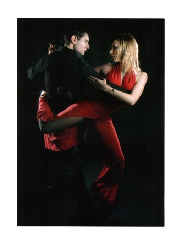
\includegraphics[width=7cm]{dance/cover_tango_book1}\tabularnewline
\tabularnewline
\tabularnewline
\tabularnewline
\end{tabular}}

\author{The TANGO Team}

\maketitle
\tableofcontents{}

\vspace{3cm}

\begin{center}
\label{FirstPicture}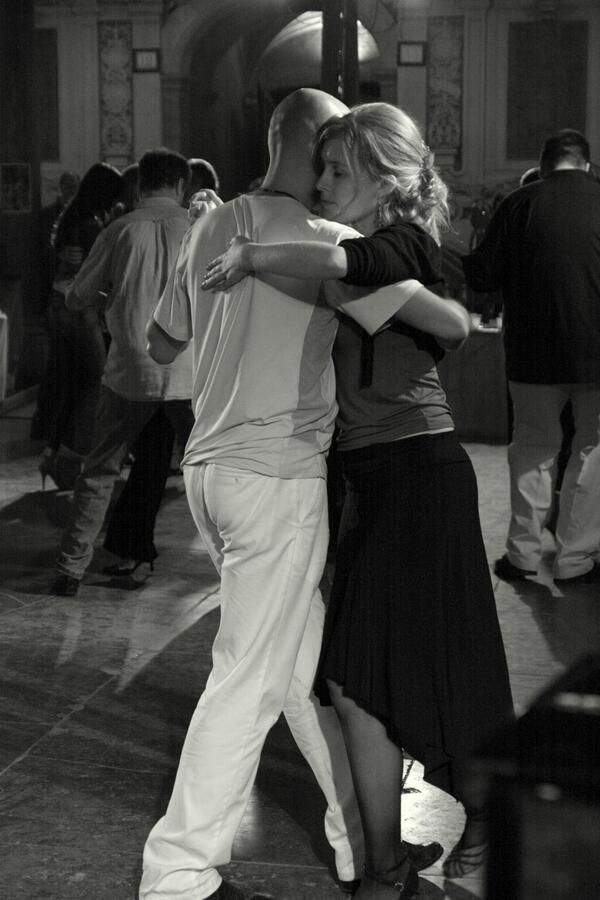
\includegraphics[scale=0.7]{dance/tango-08-27}
\par\end{center}

\vspace{0.3cm}

\begin{center}
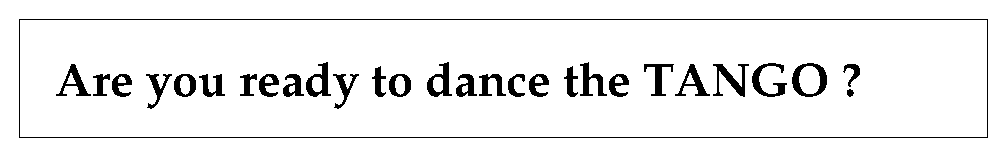
\includegraphics{dance/Ready}
\par\end{center}

\vspace{0.3cm}

\begin{comment}
Introduction 
\end{comment}


\chapter{Introduction}


\section{Introduction to device server}

Device servers were first developed at the European Synchrotron radiation
Facility (ESRF\index{ESRF}) for controlling the 6 Gev synchrotron
radiation source. This document is a Programmer's Manual on how to
write TANGO device servers. It will not go into the details of the
ESRF\index{ESRF}, nor its Control System nor any of the specific
device servers in the Control System. The role of this document is
to help programmers faced with the task of writing TANGO device servers.

Device servers have been developed at the ESRF\index{ESRF} in order
to solve the main task of Control Systems viz provide read and write
access to all devices in a distributed system. The problem of distributed
device access is only part of the problem however. The other part
of the problem is providing a programming framework for a large number
of devices programmed by a large number of programmers each having
different levels of experience and style.

Device servers have been written at the ESRF\index{ESRF} for a large
variety of different devices. Devices vary from serial line devices
to devices interfaced by field-bus to memory mapped VME cards or PC
cards to entire data acquisition systems. The definition of a device
depends very much on the user's requirements. In the simple case a
device server can be used to hide the serial line protocol required
to communicate with a device. For more complicated devices the device
server can be used to hide the entire complexity of the device timing,
configuration and acquisition cycle behind a set of high level commands.

In this manual the process of how to write TANGO client (applications)
and device servers will be treated. The manual has been organized
as follows :
\begin{itemize}
\item A getting started chapter. 
\item The TANGO device server model is treated in chapter 3 
\item Generalities on the Tango Application Programmer Interfaces are given
in chapter 4 
\item Chapter 5 is an a programmer's guide for the Tango Application ToolKit
(TangoATK). This is a Java toolkit to help Tango Java application
developers. 
\item How to write a TANGO device server is explained in chapter 6 
\item Chapter 7 describes advanced Tango features 
\end{itemize}
Throughout this manual examples of source code will be given in order
to illustrate what is meant. Most examples have been taken from the
StepperMotor class - a simulation of a stepper motor which illustrates
how a typical device server for a stepper motor at the ESRF functions.


\section{Device server history}

The concept of using device servers to access devices was first proposed
at the ESRF in 1989. It has been successfully used as the heart of
the ESRF\index{ESRF} Control System for the institute accelerator
complex. This Control System has been named TACO\index{TACO}%
\footnote{TACO stands for \textbf{T}elescope and \textbf{A}ccelerator \textbf{C}ontrolled
with \textbf{O}bjects%
}. Then, it has been decided to also used TACO to control devices in
the beam-lines. Today, more than 30 instances of TACO are running
at the ESRF. The main technologies used within TACO are the leading
technologies of the 80's. The Sun Remote Procedure Call (RPC) is used
to communicate over the network between device server and applications,
OS-9 is used on the front-end computers, C is the reference language
to write device servers and clients and the device server framework
follows the MIT Widget model. In 1999, a renewal of the control system
was started. In June 2002, Soleil\index{Soleil} and ESRF offically
decide to collaborate to develop this renewal of the old TACO control
system. Soleil is a French synchrotron radiation facility currently
under construction in the Paris suburbs. See \cite{Soleil_home_page}
to get all information about Soleil. In December 2003, Elettra\index{Elettra}
joins the club. Elettra is an Italian synchrotron radiation facility
located in Trieste. See \cite{Elettra_home_page} to get all information
about Elettra. Then, beginning of 2005, ALBA\index{ALBA} also decided
to join. ALBA is a Spanish synchrotron radiation facility located
in Barcelona. See \cite{Alba_WEB} to get all information about ALBA.
The new version of the Alba/Elettra/ESRF/Soleil control system is
named TANGO%
\footnote{TANGO stands for \textbf{TA}co \textbf{N}ext \textbf{G}eneration \textbf{O}bject%
} and is based on the 21 century technologies :
\begin{itemize}
\item CORBA\index{CORBA}%
\footnote{CORBA stands for \textbf{C}ommon \textbf{O}bject \textbf{R}equest
\textbf{B}roker \textbf{A}rchitecture%
} and ZMQ\index{ZMQ}\cite{ZMQ} to communicate between device server
and clients 
\item C++, Python and Java as reference programming languages 
\item Linux and Windows as operating systems 
\item Modern object oriented design patterns\end{itemize}



\begin{comment}
Getting started 
\end{comment}


\chapter{Getting Started}


\section{A C++ TANGO client}

\noindent The quickest way of getting started is by studying this
example :

%
% Copyright (C) :      2004,2005,2006,2007,2008,2009,2010,2011,2012,2013
%                      European Synchrotron Radiation Facility
%                      BP 220, Grenoble 38043
%                      FRANCE
%
% This file is part of Tango.
%
% Tango is free software: you can redistribute it and/or modify
% it under the terms of the GNU Lesser General Public License as published by
% the Free Software Foundation, either version 3 of the License, or
% (at your option) any later version.
%
% Tango is distributed in the hope that it will be useful,
% but WITHOUT ANY WARRANTY; without even the implied warranty of
% MERCHANTABILITY or FITNESS FOR A PARTICULAR PURPOSE.  See the
% GNU Lesser General Public License for more details.
%
% You should have received a copy of the GNU Lesser General Public License
% along with Tango.  If not, see <http://www.gnu.org/licenses/>.
%
\begin{flushleft}
\begin{picture}(0,0)
\thicklines
\put(0,0){\line(1,0){400}}
\end{picture}
\end{flushleft}

\begin{lyxcode}
\noindent /{*}~

\noindent ~{*}~example~of~a~client~using~the~TANGO~C++~api.

\noindent ~{*}/

\noindent \#include~<tango.h>

\noindent using~namespace~Tango;

\noindent int~main(unsigned~int~argc,~char~{*}{*}argv)

\noindent \{

~~~~try

~~~~\{



//

//~create~a~connection~to~a~TANGO~device

//

~

~~~~~~~~DeviceProxy~{*}device~=~new~DeviceProxy(``sys/database/2'');

~

//

//~Ping~the~device

//

~

~~~~~~~~device->ping();

~

//

//~Execute~a~command~on~the~device~and~extract~the~reply~as~a~string

//

~

~~~~~~~~string~db\_info;~

~~~~~~~~DeviceData~cmd\_reply;

~~~~~~~~cmd\_reply~=~device->command\_inout(``DbInfo'');

~~~~~~~~cmd\_reply~>\textcompwordmark{}>~db\_info;

~~~~~~~~cout~<\textcompwordmark{}<~``Command~reply~``~<\textcompwordmark{}<~db\_info~<\textcompwordmark{}<~endl;

~

//

//~Read~a~device~attribute~(string~data~type)

//

~

~~~~~~~~string~spr;

~~~~~~~~DeviceAttribute~att\_reply;

~~~~~~~~att\_reply~=~device->read\_attribute(``StoredProcedureRelease'');

~~~~~~~~att\_reply~>\textcompwordmark{}>~spr;

~~~~~~~~cout~<\textcompwordmark{}<~``Database~device~stored~procedure~release:~``~<\textcompwordmark{}<~spr~<\textcompwordmark{}<~endl;

~~~~\}

\noindent ~~~~catch~(DevFailed~\&e)

\noindent ~~~~\{

\noindent ~~~~~~~~Except::print\_exception(e);

\noindent ~~~~~~~~exit(-1);

\noindent ~~~~\}~

\noindent \}
\end{lyxcode}
%
% Copyright (C) :      2004,2005,2006,2007,2008,2009,2010,2011,2012,2013
%                      European Synchrotron Radiation Facility
%                      BP 220, Grenoble 38043
%                      FRANCE
%
% This file is part of Tango.
%
% Tango is free software: you can redistribute it and/or modify
% it under the terms of the GNU Lesser General Public License as published by
% the Free Software Foundation, either version 3 of the License, or
% (at your option) any later version.
%
% Tango is distributed in the hope that it will be useful,
% but WITHOUT ANY WARRANTY; without even the implied warranty of
% MERCHANTABILITY or FITNESS FOR A PARTICULAR PURPOSE.  See the
% GNU Lesser General Public License for more details.
%
% You should have received a copy of the GNU Lesser General Public License
% along with Tango.  If not, see <http://www.gnu.org/licenses/>.
%
\begin{flushleft}
\begin{picture}(0,0)
\thicklines
\put(0,0){\line(1,0){400}}
\end{picture}
\end{flushleft}


\noindent Modify this example to fit your device server or client's
needs, compile it and link with the library -ltango. Forget about
those painful early TANGO days when you had to learn CORBA and manipulate
Any's. Life's going to easy and fun from now on !


\section{A TANGO device server}

The code given in this chapter as example has been generated using
POGO. Pogo\index{Pogo} is a code generator for Tango device server.
See \cite{Pogo doc} for more information about POGO. The following
examples briefly describe how to write device class with commands
which receives and return different kind of Tango data types and also
how to write device attributes\index{attribute} The device class
implements 5 commands and 3 attributes. The commands are :
\begin{itemize}
\item The command \textbf{DevSimple} deals with simple Tango data type
\item The command \textbf{DevString} deals with Tango strings
\item \textbf{DevArray} receive and return an array of simple Tango data
type
\item \textbf{DevStrArray} which does not receive any data but which returns
an array of strings
\item \textbf{DevStruct} which also does not receive data but which returns
one of the two Tango composed types (DevVarDoubleStringArray)
\end{itemize}
For all these commands, the default behavior of the state machine
(command always allowed) is acceptable. The attributes are :
\begin{itemize}
\item A spectrum type attribute of the Tango string type called \textbf{StrAttr}
\item A readable attribute of the Tango::DevLong type called \textbf{LongRdAttr}.
This attribute is linked with the following writable attribute
\item A writable attribute also of the Tango::DevLong type called \textbf{LongWrAttr}.
\end{itemize}
Since release 9, a Tango device also supports pipe. This is an advanced
feature reserved for some specific cases. Therefore, there is no device
pipe example in this \textquotedbl{}Getting started\textquotedbl{}
chapter.


\subsection{The commands and attributes code}

For each command called DevXxxx, pogo generates in the device class
a method named dev\_xxx which will be executed when the command is
requested by a client. In this chapter, the name of the device class
is \emph{DocDs}


\subsubsection{The DevSimple command}

This method receives a Tango::DevFloat\index{Tango::DevFloat} type
and also returns a data of the Tango::DevFloat type which is simply
the double of the input value. The code for the method executed by
this command is the following:

%
% Copyright (C) :      2004,2005,2006,2007,2008,2009,2010,2011,2012,2013
%                      European Synchrotron Radiation Facility
%                      BP 220, Grenoble 38043
%                      FRANCE
%
% This file is part of Tango.
%
% Tango is free software: you can redistribute it and/or modify
% it under the terms of the GNU Lesser General Public License as published by
% the Free Software Foundation, either version 3 of the License, or
% (at your option) any later version.
%
% Tango is distributed in the hope that it will be useful,
% but WITHOUT ANY WARRANTY; without even the implied warranty of
% MERCHANTABILITY or FITNESS FOR A PARTICULAR PURPOSE.  See the
% GNU Lesser General Public License for more details.
%
% You should have received a copy of the GNU Lesser General Public License
% along with Tango.  If not, see <http://www.gnu.org/licenses/>.
%
\begin{flushleft}
\begin{picture}(0,0)
\thicklines
\put(0,0){\line(1,0){400}}
\end{picture}
\end{flushleft}

\begin{lyxcode}
~~~~~1~~Tango::DevFloat~DocDs::dev\_simple(Tango::DevFloat~argin)

~~~~~2~~\{

~~~~~3~~~~~~~~~~Tango::DevFloat~argout~;

~~~~~4~~~~~~~~~~DEBUG\_STREAM~<\textcompwordmark{}<~\textquotedbl{}DocDs::dev\_simple():~entering...~!\textquotedbl{}~<\textcompwordmark{}<~endl;

~~~~~5~~

~~~~~6~~~~~~~~~~//~~~~~~Add~your~own~code~to~control~device~here

~~~~~7~~

~~~~~8~~~~~~~~~~argout~=~argin~{*}~2;

~~~~~9~~~~~~~~~~return~argout;

~~~~10~~\}
\end{lyxcode}
%
% Copyright (C) :      2004,2005,2006,2007,2008,2009,2010,2011,2012,2013
%                      European Synchrotron Radiation Facility
%                      BP 220, Grenoble 38043
%                      FRANCE
%
% This file is part of Tango.
%
% Tango is free software: you can redistribute it and/or modify
% it under the terms of the GNU Lesser General Public License as published by
% the Free Software Foundation, either version 3 of the License, or
% (at your option) any later version.
%
% Tango is distributed in the hope that it will be useful,
% but WITHOUT ANY WARRANTY; without even the implied warranty of
% MERCHANTABILITY or FITNESS FOR A PARTICULAR PURPOSE.  See the
% GNU Lesser General Public License for more details.
%
% You should have received a copy of the GNU Lesser General Public License
% along with Tango.  If not, see <http://www.gnu.org/licenses/>.
%
\begin{flushleft}
\begin{picture}(0,0)
\thicklines
\put(0,0){\line(1,0){400}}
\end{picture}
\end{flushleft}


This method is fairly simple. The received data is passed to the method
as its argument. It is

doubled at line 8 and the method simply returns the result.


\subsubsection{The DevArray command}

This method receives a data of the Tango::DevVarLongArray\index{Tango::DevVarLongArray}
type and also returns a data of the Tango::DevVarLongArray type. Each
element of the array is doubled. The code for the method executed
by the command is the following :

%
% Copyright (C) :      2004,2005,2006,2007,2008,2009,2010,2011,2012,2013
%                      European Synchrotron Radiation Facility
%                      BP 220, Grenoble 38043
%                      FRANCE
%
% This file is part of Tango.
%
% Tango is free software: you can redistribute it and/or modify
% it under the terms of the GNU Lesser General Public License as published by
% the Free Software Foundation, either version 3 of the License, or
% (at your option) any later version.
%
% Tango is distributed in the hope that it will be useful,
% but WITHOUT ANY WARRANTY; without even the implied warranty of
% MERCHANTABILITY or FITNESS FOR A PARTICULAR PURPOSE.  See the
% GNU Lesser General Public License for more details.
%
% You should have received a copy of the GNU Lesser General Public License
% along with Tango.  If not, see <http://www.gnu.org/licenses/>.
%
\begin{flushleft}
\begin{picture}(0,0)
\thicklines
\put(0,0){\line(1,0){400}}
\end{picture}
\end{flushleft}

\begin{lyxcode}
~~~~~1~~Tango::DevVarLongArray~{*}DocDs::dev\_array(const~Tango::DevVarLongArray~{*}argin)

~~~~~2~~\{

~~~~~3~~~~~~~~~~//~~~~~~POGO~has~generated~a~method~core~with~argout~allocation.

~~~~~4~~~~~~~~~~//~~~~~~If~you~would~like~to~use~a~static~reference~without~copying,

~~~~~5~~~~~~~~~~//~~~~~~See~\textquotedbl{}TANGO~Device~Server~Programmer's~Manual\textquotedbl{}

~~~~~6~~~~~~~~~~//~~~~~~~~~~~~~~(chapter~x.x)

~~~~~7~~~~~~~~~~//-{}-{}-{}-{}-{}-{}-{}-{}-{}-{}-{}-{}-{}-{}-{}-{}-{}-{}-{}-{}-{}-{}-{}-{}-{}-{}-{}-{}-{}-{}-{}-{}-{}-{}-{}-{}-{}-{}-{}-{}-{}-{}-{}-{}-{}-{}-{}-{}-{}-{}-{}-{}-{}-{}-{}-{}-{}-{}-{}-

~~~~~8~~~~~~~~~~Tango::DevVarLongArray~~{*}argout~~=~new~Tango::DevVarLongArray();

~~~~~9~~~~~~~~~~~~~~~~~~

~~~~10~~~~~~~~~~DEBUG\_STREAM~<\textcompwordmark{}<~\textquotedbl{}DocDs::dev\_array():~entering...~!\textquotedbl{}~<\textcompwordmark{}<~endl;

~~~~11~~

~~~~12~~~~~~~~~~//~~~~~~Add~your~own~code~to~control~device~here

~~~~13~~

~~~~14~~~~~~~~~~long~argin\_length~=~argin->length();~~~~

~~~~15~~~~~~~~~~argout->length(argin\_length);

~~~~16~~~~~~~~~~for~(int~i~=~0;i~<~argin\_length;i++)

~~~~17~~~~~~~~~~~~~~~~~~({*}argout){[}i{]}~=~({*}argin){[}i{]}~{*}~2;

~~~~18~~

~~~~19~~~~~~~~~~return~argout;

~~~~20~~\}
\end{lyxcode}
%
% Copyright (C) :      2004,2005,2006,2007,2008,2009,2010,2011,2012,2013
%                      European Synchrotron Radiation Facility
%                      BP 220, Grenoble 38043
%                      FRANCE
%
% This file is part of Tango.
%
% Tango is free software: you can redistribute it and/or modify
% it under the terms of the GNU Lesser General Public License as published by
% the Free Software Foundation, either version 3 of the License, or
% (at your option) any later version.
%
% Tango is distributed in the hope that it will be useful,
% but WITHOUT ANY WARRANTY; without even the implied warranty of
% MERCHANTABILITY or FITNESS FOR A PARTICULAR PURPOSE.  See the
% GNU Lesser General Public License for more details.
%
% You should have received a copy of the GNU Lesser General Public License
% along with Tango.  If not, see <http://www.gnu.org/licenses/>.
%
\begin{flushleft}
\begin{picture}(0,0)
\thicklines
\put(0,0){\line(1,0){400}}
\end{picture}
\end{flushleft}


The argout data array is created at line 8. Its length is set at line
15 from the input argument length. The array is populated at line
16,17 and returned. This method allocates memory\index{memory} for
the argout array. This memory is freed by the Tango core classes after
the data have been sent to the caller (no delete is needed). It is
also possible to return data from a statically allocated array without
copying. Look at chapter \ref{Data exchange} for all the details.


\subsubsection{The DevString command}

This method receives a data of the Tango::DevString\index{Tango::DevString}
type and also returns a data of the Tango::DevString type. The command
simply displays the content of the input string and returns a hard-coded
string. The code for the method executed by the command is the following
:

%
% Copyright (C) :      2004,2005,2006,2007,2008,2009,2010,2011,2012,2013
%                      European Synchrotron Radiation Facility
%                      BP 220, Grenoble 38043
%                      FRANCE
%
% This file is part of Tango.
%
% Tango is free software: you can redistribute it and/or modify
% it under the terms of the GNU Lesser General Public License as published by
% the Free Software Foundation, either version 3 of the License, or
% (at your option) any later version.
%
% Tango is distributed in the hope that it will be useful,
% but WITHOUT ANY WARRANTY; without even the implied warranty of
% MERCHANTABILITY or FITNESS FOR A PARTICULAR PURPOSE.  See the
% GNU Lesser General Public License for more details.
%
% You should have received a copy of the GNU Lesser General Public License
% along with Tango.  If not, see <http://www.gnu.org/licenses/>.
%
\begin{flushleft}
\begin{picture}(0,0)
\thicklines
\put(0,0){\line(1,0){400}}
\end{picture}
\end{flushleft}

\begin{lyxcode}
~~~~~1~~Tango::DevString~DocDs::dev\_string(Tango::DevString~argin)

~~~~~2~~\{

~~~~~3~~~~~~~~~~//~~~~~~POGO~has~generated~a~method~core~with~argout~allocation.

~~~~~4~~~~~~~~~~//~~~~~~If~you~would~like~to~use~a~static~reference~without~copying,

~~~~~5~~~~~~~~~~//~~~~~~See~\textquotedbl{}TANGO~Device~Server~Programmer's~Manual\textquotedbl{}

~~~~~6~~~~~~~~~~//~~~~~~~~~~~~~~(chapter~x.x)

~~~~~7~~~~~~~~~~//-{}-{}-{}-{}-{}-{}-{}-{}-{}-{}-{}-{}-{}-{}-{}-{}-{}-{}-{}-{}-{}-{}-{}-{}-{}-{}-{}-{}-{}-{}-{}-{}-{}-{}-{}-{}-{}-{}-{}-{}-{}-{}-{}-{}-{}-{}-{}-{}-{}-{}-{}-{}-{}-{}-{}-{}-{}-{}-{}-

~~~~~8~~~~~~~~~~Tango::DevString~~~~~~~~argout;

~~~~~9~~~~~~~~~~DEBUG\_STREAM~<\textcompwordmark{}<~\textquotedbl{}DocDs::dev\_string():~entering...~!\textquotedbl{}~<\textcompwordmark{}<~endl;

~~~~10~~

~~~~11~~~~~~~~~~//~~~~~~Add~your~own~code~to~control~device~here

~~~~12~~

~~~~13~~~~~~~~~~cout~<\textcompwordmark{}<~\textquotedbl{}the~received~string~is~\textquotedbl{}~<\textcompwordmark{}<~argin~<\textcompwordmark{}<~endl;

~~~~14~~~~~~~~~~

~~~~15~~~~~~~~~~string~str(\textquotedbl{}Am~I~a~good~Tango~dancer~?\textquotedbl{});

~~~~16~~~~~~~~~~argout~=~new~char{[}str.size()~+~1{]};

~~~~17~~~~~~~~~~strcpy(argout,str.c\_str());

~~~~18~~~~~~~~~~

~~~~19~~~~~~~~~~return~argout;

~~~~20~~\}
\end{lyxcode}
%
% Copyright (C) :      2004,2005,2006,2007,2008,2009,2010,2011,2012,2013
%                      European Synchrotron Radiation Facility
%                      BP 220, Grenoble 38043
%                      FRANCE
%
% This file is part of Tango.
%
% Tango is free software: you can redistribute it and/or modify
% it under the terms of the GNU Lesser General Public License as published by
% the Free Software Foundation, either version 3 of the License, or
% (at your option) any later version.
%
% Tango is distributed in the hope that it will be useful,
% but WITHOUT ANY WARRANTY; without even the implied warranty of
% MERCHANTABILITY or FITNESS FOR A PARTICULAR PURPOSE.  See the
% GNU Lesser General Public License for more details.
%
% You should have received a copy of the GNU Lesser General Public License
% along with Tango.  If not, see <http://www.gnu.org/licenses/>.
%
\begin{flushleft}
\begin{picture}(0,0)
\thicklines
\put(0,0){\line(1,0){400}}
\end{picture}
\end{flushleft}


The argout string is created at line 8. Internally, this method is
using a standard C++ string. Memory for the returned data is allocated
at line 16 and is initialized at line 17. This method allocates memory\index{memory}
for the argout string. This memory is freed by the Tango core classes
after the data have been sent to the caller (no delete is needed).
It is also possible to return data from a statically allocated string
without copying. Look at chapter \ref{Data exchange} for all the
details.


\subsubsection{The DevStrArray command}

This method does not receive input data but returns an array of strings
(Tango::DevVarStringArray\index{Tango::DevVarStringArray} type).
The code for the method executed by this command is the following:

%
% Copyright (C) :      2004,2005,2006,2007,2008,2009,2010,2011,2012,2013
%                      European Synchrotron Radiation Facility
%                      BP 220, Grenoble 38043
%                      FRANCE
%
% This file is part of Tango.
%
% Tango is free software: you can redistribute it and/or modify
% it under the terms of the GNU Lesser General Public License as published by
% the Free Software Foundation, either version 3 of the License, or
% (at your option) any later version.
%
% Tango is distributed in the hope that it will be useful,
% but WITHOUT ANY WARRANTY; without even the implied warranty of
% MERCHANTABILITY or FITNESS FOR A PARTICULAR PURPOSE.  See the
% GNU Lesser General Public License for more details.
%
% You should have received a copy of the GNU Lesser General Public License
% along with Tango.  If not, see <http://www.gnu.org/licenses/>.
%
\begin{flushleft}
\begin{picture}(0,0)
\thicklines
\put(0,0){\line(1,0){400}}
\end{picture}
\end{flushleft}

\begin{lyxcode}
~~~~~1~~Tango::DevVarStringArray~{*}DocDs::dev\_str\_array()

~~~~~2~~\{

~~~~~3~~~~~~~~~~//~~~~~~POGO~has~generated~a~method~core~with~argout~allocation.

~~~~~4~~~~~~~~~~//~~~~~~If~you~would~like~to~use~a~static~reference~without~copying,

~~~~~5~~~~~~~~~~//~~~~~~See~\textquotedbl{}TANGO~Device~Server~Programmer's~Manual\textquotedbl{}

~~~~~6~~~~~~~~~~//~~~~~~~~~~~~~~(chapter~x.x)

~~~~~7~~~~~~~~~~//-{}-{}-{}-{}-{}-{}-{}-{}-{}-{}-{}-{}-{}-{}-{}-{}-{}-{}-{}-{}-{}-{}-{}-{}-{}-{}-{}-{}-{}-{}-{}-{}-{}-{}-{}-{}-{}-{}-{}-{}-{}-{}-{}-{}-{}-{}-{}-{}-{}-{}-{}-{}-{}-{}-{}-{}-{}-{}-{}-

~~~~~8~~~~~~~~~~Tango::DevVarStringArray~~~~~~~~{*}argout~~=~new~Tango::DevVarStringArray();

~~~~~9~~

~~~~10~~~~~~~~~~DEBUG\_STREAM~<\textcompwordmark{}<~\textquotedbl{}DocDs::dev\_str\_array():~entering...~!\textquotedbl{}~<\textcompwordmark{}<~endl;

~~~~11~~

~~~~12~~~~~~~~~~//~~~~~~Add~your~own~code~to~control~device~here

~~~~13~~

~~~~14~~~~~~~~~~argout->length(3);

~~~~15~~~~~~~~~~({*}argout){[}0{]}~=~CORBA::string\_dup(\textquotedbl{}Rumba\textquotedbl{});

~~~~16~~~~~~~~~~({*}argout){[}1{]}~=~CORBA::string\_dup(\textquotedbl{}Waltz\textquotedbl{});

~~~~17~~~~~~~~~~string~str(\textquotedbl{}Jerck\textquotedbl{});

~~~~18~~~~~~~~~~({*}argout){[}2{]}~=~CORBA::string\_dup(str.c\_str());

~~~~19~~~~~~~~~~return~argout;

~~~~20~~\}
\end{lyxcode}
%
% Copyright (C) :      2004,2005,2006,2007,2008,2009,2010,2011,2012,2013
%                      European Synchrotron Radiation Facility
%                      BP 220, Grenoble 38043
%                      FRANCE
%
% This file is part of Tango.
%
% Tango is free software: you can redistribute it and/or modify
% it under the terms of the GNU Lesser General Public License as published by
% the Free Software Foundation, either version 3 of the License, or
% (at your option) any later version.
%
% Tango is distributed in the hope that it will be useful,
% but WITHOUT ANY WARRANTY; without even the implied warranty of
% MERCHANTABILITY or FITNESS FOR A PARTICULAR PURPOSE.  See the
% GNU Lesser General Public License for more details.
%
% You should have received a copy of the GNU Lesser General Public License
% along with Tango.  If not, see <http://www.gnu.org/licenses/>.
%
\begin{flushleft}
\begin{picture}(0,0)
\thicklines
\put(0,0){\line(1,0){400}}
\end{picture}
\end{flushleft}


The argout data array is created at line 8. Its length is set at line
14. The array is populated at line 15,16 and 18. The last array element
is initialized from a standard C++ string created at line 17. Note
the usage of the \emph{string\_dup\index{string-dup}} function of
the CORBA namespace. This is necessary for strings array due to the
CORBA memory\index{memory} allocation schema.


\subsubsection{The DevStruct command}

This method does not receive input data but returns a structure of
the Tango::DevVarDoubleStringArray\index{Tango::DevVarDoubleStringArray}
type. This type is a composed type with an array of double and an
array of strings. The code for the method executed by this command
is the following:

%
% Copyright (C) :      2004,2005,2006,2007,2008,2009,2010,2011,2012,2013
%                      European Synchrotron Radiation Facility
%                      BP 220, Grenoble 38043
%                      FRANCE
%
% This file is part of Tango.
%
% Tango is free software: you can redistribute it and/or modify
% it under the terms of the GNU Lesser General Public License as published by
% the Free Software Foundation, either version 3 of the License, or
% (at your option) any later version.
%
% Tango is distributed in the hope that it will be useful,
% but WITHOUT ANY WARRANTY; without even the implied warranty of
% MERCHANTABILITY or FITNESS FOR A PARTICULAR PURPOSE.  See the
% GNU Lesser General Public License for more details.
%
% You should have received a copy of the GNU Lesser General Public License
% along with Tango.  If not, see <http://www.gnu.org/licenses/>.
%
\begin{flushleft}
\begin{picture}(0,0)
\thicklines
\put(0,0){\line(1,0){400}}
\end{picture}
\end{flushleft}

\begin{lyxcode}
~~~~~1~~Tango::DevVarDoubleStringArray~{*}DocDs::dev\_struct()

~~~~~2~~\{

~~~~~3~~~~~~~~~~//~~~~~~POGO~has~generated~a~method~core~with~argout~allocation.

~~~~~4~~~~~~~~~~//~~~~~~If~you~would~like~to~use~a~static~reference~without~copying,

~~~~~5~~~~~~~~~~//~~~~~~See~\textquotedbl{}TANGO~Device~Server~Programmer's~Manual\textquotedbl{}

~~~~~6~~~~~~~~~~//~~~~~~~~~~~~~~(chapter~x.x)

~~~~~7~~~~~~~~~~//-{}-{}-{}-{}-{}-{}-{}-{}-{}-{}-{}-{}-{}-{}-{}-{}-{}-{}-{}-{}-{}-{}-{}-{}-{}-{}-{}-{}-{}-{}-{}-{}-{}-{}-{}-{}-{}-{}-{}-{}-{}-{}-{}-{}-{}-{}-{}-{}-{}-{}-{}-{}-{}-{}-{}-{}-{}-{}-{}-

~~~~~8~~~~~~~~~~Tango::DevVarDoubleStringArray~~{*}argout~~=~new~Tango::DevVarDoubleStringArray();

~~~~~9~~

~~~~10~~~~~~~~~~DEBUG\_STREAM~<\textcompwordmark{}<~\textquotedbl{}DocDs::dev\_struct():~entering...~!\textquotedbl{}~<\textcompwordmark{}<~endl;

~~~~11~~~~~~~~~~

~~~~12~~~~~~~~~~//~~~~~~Add~your~own~code~to~control~device~here

~~~~13~~

~~~~14~~~~~~~~~~argout->dvalue.length(3);

~~~~15~~~~~~~~~~argout->dvalue{[}0{]}~=~0.0;

~~~~16~~~~~~~~~~argout->dvalue{[}1{]}~=~11.11;

~~~~17~~~~~~~~~~argout->dvalue{[}2{]}~=~22.22;

~~~~18~~~~~~~~~~

~~~~19~~~~~~~~~~argout->svalue.length(2);

~~~~20~~~~~~~~~~argout->svalue{[}0{]}~=~CORBA::string\_dup(\textquotedbl{}Be~Bop\textquotedbl{});

~~~~21~~~~~~~~~~string~str(\textquotedbl{}Smurf\textquotedbl{});

~~~~22~~~~~~~~~~argout->svalue{[}1{]}~=~CORBA::string\_dup(str.c\_str());

~~~~23~~~~~~~~~~

~~~~24~~~~~~~~~~return~argout;

~~~~25~~\}
\end{lyxcode}
%
% Copyright (C) :      2004,2005,2006,2007,2008,2009,2010,2011,2012,2013
%                      European Synchrotron Radiation Facility
%                      BP 220, Grenoble 38043
%                      FRANCE
%
% This file is part of Tango.
%
% Tango is free software: you can redistribute it and/or modify
% it under the terms of the GNU Lesser General Public License as published by
% the Free Software Foundation, either version 3 of the License, or
% (at your option) any later version.
%
% Tango is distributed in the hope that it will be useful,
% but WITHOUT ANY WARRANTY; without even the implied warranty of
% MERCHANTABILITY or FITNESS FOR A PARTICULAR PURPOSE.  See the
% GNU Lesser General Public License for more details.
%
% You should have received a copy of the GNU Lesser General Public License
% along with Tango.  If not, see <http://www.gnu.org/licenses/>.
%
\begin{flushleft}
\begin{picture}(0,0)
\thicklines
\put(0,0){\line(1,0){400}}
\end{picture}
\end{flushleft}


The argout data structure is created at line 8. The length of the
double array in the output structure is set at line 14. The array
is populated between lines 15 and 17. The length of the string array
in the output structure is set at line 19. This string array is populated
between lines 20 an 22 from a hard-coded string and from a standard
C++ string. This method allocates memory\index{memory} for the argout
data. This memory is freed by the Tango core classes after the data
have been sent to the caller (no delete is needed). Note the usage
of the \emph{string\_dup\index{string-dup}} function of the CORBA
namespace. This is necessary for strings array due to the CORBA memory
allocation schema.


\subsubsection{The three attributes\index{attribute}}

Some data have been added to the definition of the device class in
order to store attributes value. These data are (part of the class
definition) :

%
% Copyright (C) :      2004,2005,2006,2007,2008,2009,2010,2011,2012,2013
%                      European Synchrotron Radiation Facility
%                      BP 220, Grenoble 38043
%                      FRANCE
%
% This file is part of Tango.
%
% Tango is free software: you can redistribute it and/or modify
% it under the terms of the GNU Lesser General Public License as published by
% the Free Software Foundation, either version 3 of the License, or
% (at your option) any later version.
%
% Tango is distributed in the hope that it will be useful,
% but WITHOUT ANY WARRANTY; without even the implied warranty of
% MERCHANTABILITY or FITNESS FOR A PARTICULAR PURPOSE.  See the
% GNU Lesser General Public License for more details.
%
% You should have received a copy of the GNU Lesser General Public License
% along with Tango.  If not, see <http://www.gnu.org/licenses/>.
%
\begin{flushleft}
\begin{picture}(0,0)
\thicklines
\put(0,0){\line(1,0){400}}
\end{picture}
\end{flushleft}

\begin{lyxcode}
~~~~~1~~

~~~~~2~~

~~~~~3~~protected~:~~~~~

~~~~~4~~~~~~~~~~//~~~~~~Add~your~own~data~members~here

~~~~~5~~~~~~~~~~//-{}-{}-{}-{}-{}-{}-{}-{}-{}-{}-{}-{}-{}-{}-{}-{}-{}-{}-{}-{}-{}-{}-{}-{}-{}-{}-{}-{}-{}-{}-{}-{}-{}-{}-{}-{}-{}-{}-{}-{}-

~~~~~6~~~~~~~~~~Tango::DevString~~~~~~~~attr\_str\_array{[}5{]};

~~~~~7~~~~~~~~~~Tango::DevLong~~~~~~~~~~attr\_rd;

~~~~~8~~~~~~~~~~Tango::DevLong~~~~~~~~~~attr\_wr;
\end{lyxcode}
%
% Copyright (C) :      2004,2005,2006,2007,2008,2009,2010,2011,2012,2013
%                      European Synchrotron Radiation Facility
%                      BP 220, Grenoble 38043
%                      FRANCE
%
% This file is part of Tango.
%
% Tango is free software: you can redistribute it and/or modify
% it under the terms of the GNU Lesser General Public License as published by
% the Free Software Foundation, either version 3 of the License, or
% (at your option) any later version.
%
% Tango is distributed in the hope that it will be useful,
% but WITHOUT ANY WARRANTY; without even the implied warranty of
% MERCHANTABILITY or FITNESS FOR A PARTICULAR PURPOSE.  See the
% GNU Lesser General Public License for more details.
%
% You should have received a copy of the GNU Lesser General Public License
% along with Tango.  If not, see <http://www.gnu.org/licenses/>.
%
\begin{flushleft}
\begin{picture}(0,0)
\thicklines
\put(0,0){\line(1,0){400}}
\end{picture}
\end{flushleft}


One data has been created for each attribute. As the StrAttr attribute
is of type spectrum with a maximum X dimension of 5, an array of length
5 has been reserved.

Several methods are necessary to implement these attributes. One method
to read the hardware which is common to all \textquotedbl{}readable\textquotedbl{}
attributes plus one \textquotedbl{}read\textquotedbl{} method for
each readable attribute and one \textquotedbl{}write\textquotedbl{}
method for each writable attribute. The code for these methods is
the following :

%
% Copyright (C) :      2004,2005,2006,2007,2008,2009,2010,2011,2012,2013
%                      European Synchrotron Radiation Facility
%                      BP 220, Grenoble 38043
%                      FRANCE
%
% This file is part of Tango.
%
% Tango is free software: you can redistribute it and/or modify
% it under the terms of the GNU Lesser General Public License as published by
% the Free Software Foundation, either version 3 of the License, or
% (at your option) any later version.
%
% Tango is distributed in the hope that it will be useful,
% but WITHOUT ANY WARRANTY; without even the implied warranty of
% MERCHANTABILITY or FITNESS FOR A PARTICULAR PURPOSE.  See the
% GNU Lesser General Public License for more details.
%
% You should have received a copy of the GNU Lesser General Public License
% along with Tango.  If not, see <http://www.gnu.org/licenses/>.
%
\begin{flushleft}
\begin{picture}(0,0)
\thicklines
\put(0,0){\line(1,0){400}}
\end{picture}
\end{flushleft}

\begin{lyxcode}
1~void~DocDs::read\_attr\_hardware(vector<long>~\&attr\_list)

2~\{

3~~~~~DEBUG\_STREAM~<\textcompwordmark{}<~\textquotedbl{}DocDs::read\_attr\_hardware(vector<long>~\&attr\_list)~entering...~\textquotedbl{}<\textcompwordmark{}<~endl;

4~//~Add~your~own~code~here

5~

6~~~~~string~att\_name;

7~~~~~for~(long~i~=~0;i~<~attr\_list.size();i++)

8~~~~~\{

9~~~~~~~~~att\_name~=~dev\_attr->get\_attr\_by\_ind(attr\_list{[}i{]}).get\_name();

10~

11~~~~~~~~if~(att\_name~==~\textquotedbl{}LongRdAttr\textquotedbl{})

12~~~~~~~~\{

13~~~~~~~~~~~~attr\_rd~=~5;

14~~~~~~~~\}

15~~~~\}

16~\}

17~

18~void~DocDs::read\_LongRdAttr(Tango::Attribute~\&attr)

19~\{

20~~~~~DEBUG\_STREAM~<\textcompwordmark{}<~\textquotedbl{}DocDs::read\_LongRdAttr(Tango::Attribute~\&attr)~entering...~\textquotedbl{}<\textcompwordmark{}<~endl;

21~

22~~~~~attr.set\_value(\&attr\_rd);

23~\}

24~

25~void~DocDs::read\_LongWrAttr(Tango::Attribute~\&attr)

26~\{

27~~~~~DEBUG\_STREAM~<\textcompwordmark{}<~\textquotedbl{}DocDs::read\_LongWrAttr(Tango::Attribute~\&attr)~entering...~\textquotedbl{}<\textcompwordmark{}<~endl;

28~

29~~~~~attr.set\_value(\&attr\_wr);

30~\}

31~

32~void~DocDs::write\_LongWrAttr(Tango::WAttribute~\&attr)

33~\{

34~~~~~DEBUG\_STREAM~<\textcompwordmark{}<~\textquotedbl{}DocDs::write\_LongWrAttr(Tango::WAttribute~\&attr)~entering...~\textquotedbl{}<\textcompwordmark{}<~endl;

35~

36~~~~~attr.get\_write\_value(attr\_wr);

37~~~~~DEBUG\_STREAM~<\textcompwordmark{}<~\textquotedbl{}Value~to~be~written~=~\textquotedbl{}~<\textcompwordmark{}<~attr\_wr~<\textcompwordmark{}<~endl;

38~\}

39~

40~void~DocDs::read\_StrAttr(Tango::Attribute~\&attr)

41~\{

42~~~~~DEBUG\_STREAM~<\textcompwordmark{}<~\textquotedbl{}DocDs::read\_StrAttr(Tango::Attribute~\&attr)~entering...~\textquotedbl{}<\textcompwordmark{}<~endl;

43~

44~~~~~attr\_str\_array{[}0{]}~=~const\_cast<char~{*}>(\textquotedbl{}Rock\textquotedbl{});

45~~~~~attr\_str\_array{[}1{]}~=~const\_cast<char~{*}>(\textquotedbl{}Samba\textquotedbl{});

46~

47~~~~~attr\_set\_value(attr\_str\_array,~2);

48~\}
\end{lyxcode}
%
% Copyright (C) :      2004,2005,2006,2007,2008,2009,2010,2011,2012,2013
%                      European Synchrotron Radiation Facility
%                      BP 220, Grenoble 38043
%                      FRANCE
%
% This file is part of Tango.
%
% Tango is free software: you can redistribute it and/or modify
% it under the terms of the GNU Lesser General Public License as published by
% the Free Software Foundation, either version 3 of the License, or
% (at your option) any later version.
%
% Tango is distributed in the hope that it will be useful,
% but WITHOUT ANY WARRANTY; without even the implied warranty of
% MERCHANTABILITY or FITNESS FOR A PARTICULAR PURPOSE.  See the
% GNU Lesser General Public License for more details.
%
% You should have received a copy of the GNU Lesser General Public License
% along with Tango.  If not, see <http://www.gnu.org/licenses/>.
%
\begin{flushleft}
\begin{picture}(0,0)
\thicklines
\put(0,0){\line(1,0){400}}
\end{picture}
\end{flushleft}


The \emph{read\_attr\_hardware\index{read-attr-hardware}()} method
is executed once when a client execute the read\_attributes\index{read-attributes}
CORBA request whatever the number of attribute to be read is. The
rule of this method is to read the hardware and to store the read
values somewhere in the device object. In our example, only the LongRdAttr
attribute internal value is set by this method at line 13. The method
\emph{read\_LongRdAttr()} is executed by the read\_attributes\index{read-attributes}
CORBA call when the LongRdAttr attribute is read but after the read\_attr\_hardware()
method has been executed. Its rule is to set the attribute value in
the TANGO core classes object representing the attribute. This is
done at line 22. The method \emph{read\_LongWrAttr()} will be executed
when the LongWrAttr attribute is read (after the \emph{read\_attr\_hardware()}
method). The attribute value is set at line 29. In the same manner,
the method called \emph{read\_StrAttr()} will be executed when the
attribute StrAttr is read. Its value is initialized in this method
at line 44 and 45 with the \emph{string\_dup\index{string-dup}} Tango
function. There are several ways to code spectrum or image attribute
of the DevString data type. A HowTo related to this topic is available
on the Tango control system Web site. The \emph{write\_LongWrAttr()}
method is executed when the LongWrAttr attribute\index{attribute}
value is set by a client. The new attribute value coming from the
client is stored in the object data at line 36.

Pogo also generates a file called \textquotedbl{}DocDsStateMachine.cpp\textquotedbl{}
(for a Tango device server class called DocDs). This file is used
to store methods coding the device state machine. By default a allways
allowed state machine is provided. For more information about coding
the state machine, refer to the chapter \textquotedbl{}Writing a device
server\textquotedbl{}.

\newpage{}

\vspace{5cm}


\begin{center}
\label{APicture}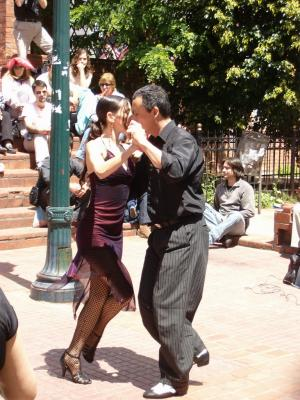
\includegraphics{dance/tg_argentine}
\par\end{center}


\begin{comment}
The TANGO device server model 
\end{comment}


\chapter{The TANGO device server model}

This chapter will present the TANGO device server object model hereafter
referred as TDSOM\index{TDSOM}. First, it will introduce CORBA\index{CORBA}.
Then, it will describe each of the basic features of the TDSOM and
their function. The TDSOM can be divided into the following basic
elements - the \emph{device}, the \emph{server}, the \emph{database}
and the \emph{application programmers interface}. This chapter will
treat each of the above elements separately.


\section{Introduction to CORBA\label{sec:corba}}

CORBA is a definition of how to write object request brokers (ORB\index{ORB}).
The definition is managed by the Object Management Group (OMG\index{OMG}
\cite{OMG-page}). Various commercial and non-commercial implementations
exist for CORBA for all the mainstream operating systems. CORBA\index{CORBA}
uses a programming language independent definition language (called
IDL) to defined network object interfaces. Language mappings are defined
from IDL\index{IDL} to the main programming languages e.g. C++, Java,
C, COBOL, Smalltalk and ADA. Within an interface, CORBA defines two
kinds of actions available to the outside world. These actions are
called \textbf{attributes\index{attribute}} and \textbf{operations}\index{operation}.

Operations are all the actions offered by an interface. For instance,
within an interface for a Thermostat class, operations could be the
action to read the temperature or to set the nominal temperature.
An attribute defines a pair of operations a client can call to send
or receive a value. For instance, the position of a motor can be defined
as an attribute because it is a data that you only set or get. A read
only attribute defines a single operation the client can call to receives
a value. In case of error, an operation is able to throw an exception
to the client, attributes cannot raises exception except system exception
(du to network fault for instance).

Intuitively, IDL interface correspond to C++ classes and IDL operations
correspond to C++ member functions and attributes as a way to read/write
public member variable. Nevertheless, IDL defines only the interface
to an object and say nothing about the object implementation. IDL
is only a descriptive language. Once the interface is fully described
in the IDL language, a compiler (from IDL to C++, from IDL to Java...)
generates code to implement this interface. Obviously, you still have
to write how operations are implemented.

The act of invoking an operation on an interface causes the ORB to
send a message to the corresponding object implementation. If the
target object is in another address space, the ORB run time sends
a remote procedure call to the implementation. If the target object
is in the same address space as the caller, the invocation is accomplished
as an ordinary function call to avoid the overhead of using a networking
protocol.

For an excellent reference on CORBA\index{CORBA} with C++ refer to
\cite{Henning}. The complete TANGO IDL\index{IDL} file can be found
in the TANGO web page\cite{Tango web} or at the end of this document
in the appendix 2 chapter.


\section{The model}

The basic idea of the TDSOM\index{TDSOM} is to treat each device
as an \textbf{object}. Each device is a separate entity which has
its own data and behavior. Each device has a unique name which identifies
it in network name space. Devices are organized according to \textbf{classes},
each device belonging to a class. All classes are derived from one
root class thus allowing some common behavior for all devices. Four
kind of requests can be sent to a device (locally i.e. in the same
process, or remotely i.e. across the network) :
\begin{itemize}
\item Execute actions via \textbf{commands\index{command}}
\item Read/Set data specific to each device belonging to a class via TANGO
\textbf{attributes\index{attribute}}
\item Read/Set data specific to each device belonging to a class via TANGO
\textbf{pipes}\index{pipe}
\item Read some basic device data available for all devices via CORBA attributes.
\item Execute a predefined set of actions available for every devices via
CORBA operations\index{operation}
\end{itemize}
Each device is stored in a process called a \textbf{device server}\index{server}.
Devices are configured at runtime via \textbf{properties\index{properties}}
which are stored in a \textbf{database}\index{database}.


\section{The device\label{sec:dev}}

The device is the heart of the TDSOM. A device is an abstract concept
defined by the TDSOM. In reality, it can be a piece of hardware (an
interlock bit) a collection of hardware (a screen attached to a stepper
motor) a logical device (a taper) or a combination of all these (an
accelerator). Each device has a unique name in the control system
and eventually one alias\index{alias}. Within Tango, a four field
name\index{name} space has been adopted consisting of \begin{center}{[}//FACILITY/{]}DOMAIN/CLASS/MEMBER\end{center}
Facility refers to the control system instance, domain refers to the
sub-system, class the class and member the instance of the device.
Device name alias(es) must also be unique within a control system.
There is no predefined syntax for device name alias.

Each device belongs to a class. The device class contains a complete
description and implementation of the behavior of all members of that
class. New device classes can be constructed out of existing device
classes. This way a new hierarchy of classes can be built up in a
short time. Device classes can use existing devices as sub-classes
or as sub-objects. The practice of reusing existing classes is classical
for Object Oriented Programming and is one of its main advantages.

All device classes are derived from the same class (the device root
class) and implement \textbf{the same CORBA interface}. All devices
implementing the same CORBA interface ensures all control object support
the same set of CORBA operations and attributes. The device root class
contains part of the common device code. By inheriting from this class,
all devices shared a common behavior. This also makes maintenance
and improvements to the TDSOM easy to carry out.

All devices also support a \textbf{black box\index{black-box}} where
client requests for attributes or operations are recorded. This feature
allows easier debugging session for device already installed in a
running control system.


\subsection{The commands\index{command}}

Each device class implements a list of commands. Commands are very
important because they are the client's major dials and knobs for
controlling a device. Commands have a fixed calling syntax - consisting
of one input argument and one output argument. Arguments type must
be chosen in a fixed set of data types: All simple types (boolean,
short, long (32 bits), long (64 bits), float, double, unsigned short,
unsigned long (32 bits), unsigned long (64 bits) and string) and arrays
of simple types plus array of strings and longs and array of strings
and doubles). Commands can execute any sequence of actions. Commands
can be executed synchronously (the requester is blocked until the
command ended) or asynchronously (the requester send the request and
is called back when the command ended).

Commands are executed using two CORBA operations named \textbf{command\_inout\index{command-inout}}
for synchronous commands and \textbf{command\_inout\_async\index{command-inout-async}}
for asynchronous commands. These two operations called a special method
implemented in the device root class - the \emph{command\_handler\index{command-handler}}
method. The \emph{command\_handler} calls an \emph{is\_allowed\index{is-allowed}}
method implemented in the device class before calling the command
itself. The \emph{is\_allowed} method is specific to each command%
\footnote{In contrary to the state\_handler method of the TACO device server
model which is not specific to each command.%
}. It checks to see whether the command to be executed is compatible
with the present device state. The command function is executed only
if the \emph{is\_allowed} method allows it. Otherwise, an exception
is sent to the client.


\subsection{The TANGO attributes\index{attribute}}

In addition to commands, TANGO devices also support normalized data
types called attributes%
\footnote{TANGO attributes were known as signals in the TACO device server model%
}. Commands are device specific and the data they transport are not
normalized i.e. they can be any one of the TANGO data types with no
restriction on what each byte means. This means that it is difficult
to interpret the output of a command\index{command} in terms of what
kind of value(s) it represents. Generic display programs need to know
what the data returned represents, in what units it is, plus additional
information like minimum, maximum, quality etc. Tango attributes solve
this problem.

TANGO attributes are zero, one or two dimensional data which have
a fix set of properties e.g. quality, minimum and maximum, alarm low
and high. They are transferred in a specialized TANGO type and can
be read, write or read-write. A device can support a list of attributes.
Clients can read one or more attributes from one or more devices.
To read TANGO attributes, the client uses the \textbf{read\_attributes\index{read-attributes}}
operation. To write TANGO attributes, a client uses the \textbf{write\_attributes\index{write-attributes}}
operation. To write then read TANGO attributes within the same network
request, the client uses the \textbf{write\_read\_attributes\index{write-read-attribute}}
operation. To query a device for all the attributes it supports, a
client uses the \textbf{get\_attribute\_config\index{get-attribute-config}}
operation. A client is also able to modify some of parameters defining
an attribute with the \textbf{set\_attribute\_config\index{set-attribute-config}}
operation. These five operations are defined in the device CORBA interface.

TANGO support thirteen data types for attributes (and arrays of for
one or two dimensional data) which are: boolean, short, long (32 bits),
long (64 bits), float, double, unsigned char, unsigned short, unsigned
long (32 bits), unsigned long (64 bits), string, a specific data type
for Tango device state and finally another specific data type to transfer
data as an array of unsigned char with a string describing the coding
of these data.


\subsection{The TANGO pipes\index{pipe}}

Since release 9, in addition to commands and attributes, TANGO devices
also support pipes.

In some cases, it is required to exchange data between client and
device of varrying data type. This is for instance the case of data
gathered during a scan on one experiment. Because the number of actuators
and sensors involved in the scan may change from one scan to another,
it is not possible to use a well defined data type. TANGO pipes have
been designed for such cases. A TANGO pipe is basically a pipe dedicated
to transfer data between client and device. A pipe has a set of two
properties which are the pipe label and its description. A pipe can
be read or read-write. A device can support a list of pipes. Clients
can read one or more pipes from one or more devices. To read a TANGO
pipe, the client uses the \textbf{read\_pipe\index{read-pipe}} operation.
To write a TANGO pipe, a client uses the \textbf{write\_pipe\index{write-pipe}}
operation. To write then read a TANGO pipe within the same network
request, the client uses the \textbf{write\_read\_pipe\index{write-read-pipe}}
operation. To query a device for all the pipes it supports, a client
uses the \textbf{get\_pipe\_config\index{get-pipe-config}} operation.
A client is also able to modify some of parameters defining a pipe
with the \textbf{set\_pipe\_config\index{set-pipe-config}} operation.
These five operations are defined in the device CORBA interface.

In contrary of commands or attributes, a TANGO pipe does not have
a pre-defined data type. Data transferred through pipes may be of
any basic Tango data type (or array of) and this may change every
time a pipe is read or written. 


\subsection{Command, attributes or pipes ?}

There are no strict rules concerning what should be returned as command
result and what should be implemented as an attribute or as a pipe.
Nevertheless, attributes are more adapted to return physical value
which have a kind of time consistency. Attribute also have more properties
which help the client to precisely know what it represents. For instance,
the state and the status of a power supply are not physical values
and are returned as command result. The current generated by the power
supply is a physical value and is implemented as an attribute. The
attribute properties allow a client to know its unit, its label and
some other informations which are related to a physical value. Command
are well adapted to send order to a device like switching from one
mode of operation to another mode of operation. For a power supply,
the switch from a STANDBY mode to a ON mode is typically done via
a command. Finally pipe is well adapted when the kind and number of
data exchanged between the client and the device change with time.


\subsection{The CORBA attributes}

Some key data implemented for each device can be read without the
need to call a command or read an attribute. These data are :
\begin{itemize}
\item The device state\index{state}
\item The device status\index{status}
\item The device name\index{name}
\item The administration device name called adm\_name\index{administration}
\item The device description\index{description}
\end{itemize}
The device state is a number representing its state. A set of predefined
states are defined in the TDSOM. The device status is a string describing
in plain text the device state and any additional useful information
of the device as a formatted ascii string. The device name is its
name as defined in \ref{sec:dev}. For each set of devices grouped
within the same server, an administration device is automatically
added. This adm\_name is the name of the administration device. The
device description is also an ascii string describing the device rule.

These five CORBA attributes are implemented in the device root class
and therefore do not need any coding from the device class programmer.
As explained in \ref{sec:corba}, the CORBA attributes are not allowed
to raise exceptions whereas command (which are implemented using CORBA
operations) can.


\subsection{The remaining CORBA operations}

The TDSOM also supports a list of actions defined as CORBA operations
in the device interface and implemented in the device root class.
Therefore, these actions are implemented automatically for every TANGO
device. These operations are :
\begin{lyxlist}{MMMMMMMMMMM}
\item [{ping\index{ping}}] to ping a device to check if the device is
alive. Obviously, it checks only the connection from a client to the
device and not all the device functionalities
\item [{command\_list\_query\index{command-list-query}}] request a list
of all the commands supported by a device with their input and output
types and description
\item [{command\_query\index{command-query}}] request information about
a specific command which are its input and output type and description
\item [{info\index{info}}] request general information on the device like
its name, the host where the device server hosting the device is running...
\item [{black\_box\index{black-box}}] read the device black-box as an
array of strings
\end{lyxlist}

\subsection{The special case of the device state and status}

Device state\index{state} and status\index{status} are the most
important key device informations. Nearly all client software dealing
with Tango device needs device(s) state and/or status. In order to
simplify client software developper work, it is possible to get these
two piece of information in three different manners :
\begin{enumerate}
\item Using the appropriate CORBA attribute (state or status)
\item Using command on the device. The command are called State or Status
\item Using attribute. Even if the state and status are not real attribute,
it is possible to get their value using the read\_attributes operation.
Nevertheless, it is not possible to set the attribute configuration
for state and status. An error is reported by the server if a client
try to do so.
\end{enumerate}

\subsection{The device polling\index{polling}}

Within the Tango framework, it is also possible to force executing
command(s) or reading attribute(s) at a fixed frequency. It is called
\emph{device polling}. This is automatically handled by Tango core
software with a polling threads pool. The command result or attribute
value are stored in circular buffers. When a client want to read attribute
value (or command result) for a polled attribute (or a polled command),
he has the choice to get the attribute value (or command result) with
a real access to the device of from the last value stored in the device
ring buffer. This is a great advantage for ``slow'' devices. Getting
data from the buffer is much faster than accessing the device itself.
The technical disadvantage is the time shift between the data returned
from the polling buffer and the time of the request. Polling a command
is only possible for command without input arguments. It is not possible
to poll a device pipe\index{pipe}.

Two other CORBA operations called \emph{command\_inout\_history\_X\index{command-inout-history-X}}
and \emph{read\_attribute \_history\_X\index{read-attribute-history-X}}
allow a client to retrieve the history of polled command or attribute
stored in the polling buffers. Obviously, this history is limited
to the depth of the polling buffer. 

The whole polling system is available only since Tango release 2.x
and above in CPP and since TangORB release 3.7.x and above in Java.


\section{The server}

Another integral part of the TDSOM is the server concept. The server
(also referred as device server\index{server}) is a process whose
main task is to offer one or more services to one or more clients.
To do this, the server has to spend most of its time in a wait loop
waiting for clients to connect to it. The devices are hosted in the
server process. A server is able to host several classes of devices.
In the TDSOM, a device of the \textbf{DServer} class is automatically
hosted by each device server. This class of device supports commands
which enable remote device server process administration.

TANGO supports device server process on two families of operating
system : Linux and Windows.


\section{The Tango Logging\index{logging} Service\label{sec:The-Tango-Logging}}

During software life, it is always convenient to print miscellaneous
informations which help to:
\begin{itemize}
\item Debug the software
\item Report on error
\item Give regular information to user
\end{itemize}
This is classically done using cout (or C printf) in C++ or println
method in Java language. In a highly distributed control system, it
is difficult to get all these informations coming from a high number
of different processes running on a large number of computers. Since
its release 3, Tango has incorporated a Logging Service called the
Tango Logging Service (TLS) which allows print messages to be:
\begin{itemize}
\item Displayed on a console (the classical way)
\item Sent to a file
\item Sent to specific Tango device called log consumer\index{consumer}.
Tango package has an implementation of log consumer where every consumer
device is associated to a graphical interface. This graphical interface
display messages but could also be used to sort messages, to filter
messages... Using this feature, it is possible to centralise display
of these messages coming from different devices embedded within different
processes. These log consumers can be:

\begin{itemize}
\item Statically configured meaning that it memorizes the list of Tango
devices for which it will get and display messages.
\item Dynamically configured. The user, with the help of the graphical interface,
chooses devices from which he want to see messages.
\end{itemize}
\end{itemize}

\section{The database\index{database}}

To achieve complete device independence, it is necessary however to
supplement device classes with a possibility for configuring device
dependencies at runtime. The utility which does this in the TDSOM
is the \textbf{property database}. Properties%
\footnote{Properties were known as resources in the TACO device server model%
} are identified by an ascii string and the device name. TANGO attributes\index{attribute}
are also configured using properties\index{properties}. This database
is also used to store device network addresses (CORBA IOR\index{IOR}'s),
list of classes hosted by a device server process and list of devices
for each class in a device server process. The database ensure the
uniqueness of device name and of alias. It also links device name
and it list of aliases.

TANGO uses MySQL\index{MySQL}\cite{mysql} as its database. MySQL
is a relational database which implements the SQL language. However,
this is largely enough to implement all the functionalities needed
by the TDSOM. The database is accessed via a classical TANGO device
hosted in a device server. Therefore, client access the database via
TANGO commands requested on the database device. For a good reference
on MySQL refer to \cite{MySQL book}


\section{The controlled access}

Tango also provides a controlled access\index{controlled-access}
system. It's a simple controlled access system. It does not provide
encrypted communication or sophisticated authentification. It simply
defines which user (based on computer loggin authentification) is
allowed to do which command (or write attribute) on which device and
from which host. The information used to configure this controlled
access feature are stored in the Tango database and accessed by a
specific Tango device server which is not the classsical Tango database
device server described in the previous section. Two access levels
are defined:
\begin{itemize}
\item Everything is allowed for this user from this host
\item The write-like calls on the device are forbidden and according to
configuration, a command subset is also forbidden for this user from
this host
\end{itemize}
This feature is precisely described in the chapter \textquotedbl{}Advanced
features\textquotedbl{}


\section{The Application Programmers Interfaces}


\subsection{Rules of the API}

While it is true TANGO clients can be programmed using only the CORBA
API, CORBA knows nothing about TANGO. This means client have to know
all the details of retrieving IORs from the TANGO database, additional
information to send on the wire, TANGO version control etc. These
details can and should be wrapped in TANGO Application Programmer
Interface (API). The API is implemented as a library in C++ and as
a package in Java. The API is what makes TANGO clients easy to write.
The API's consists the following basic classes :
\begin{itemize}
\item DeviceProxy which is a \emph{proxy} to the real device
\item DeviceData to encapsulate data send/receive from/to device via commands
\item DeviceAttribute to encapsulate data send/receive from/to device via
attributes
\item Group which is a \emph{proxy} to a group\index{group} of devices
\end{itemize}
In addition to these main classes, many other classes allows a full
interface to TANGO features. The following figure is a drawing of
a typical client/server application using TANGO.

\vspace{0.3cm}


\begin{center}
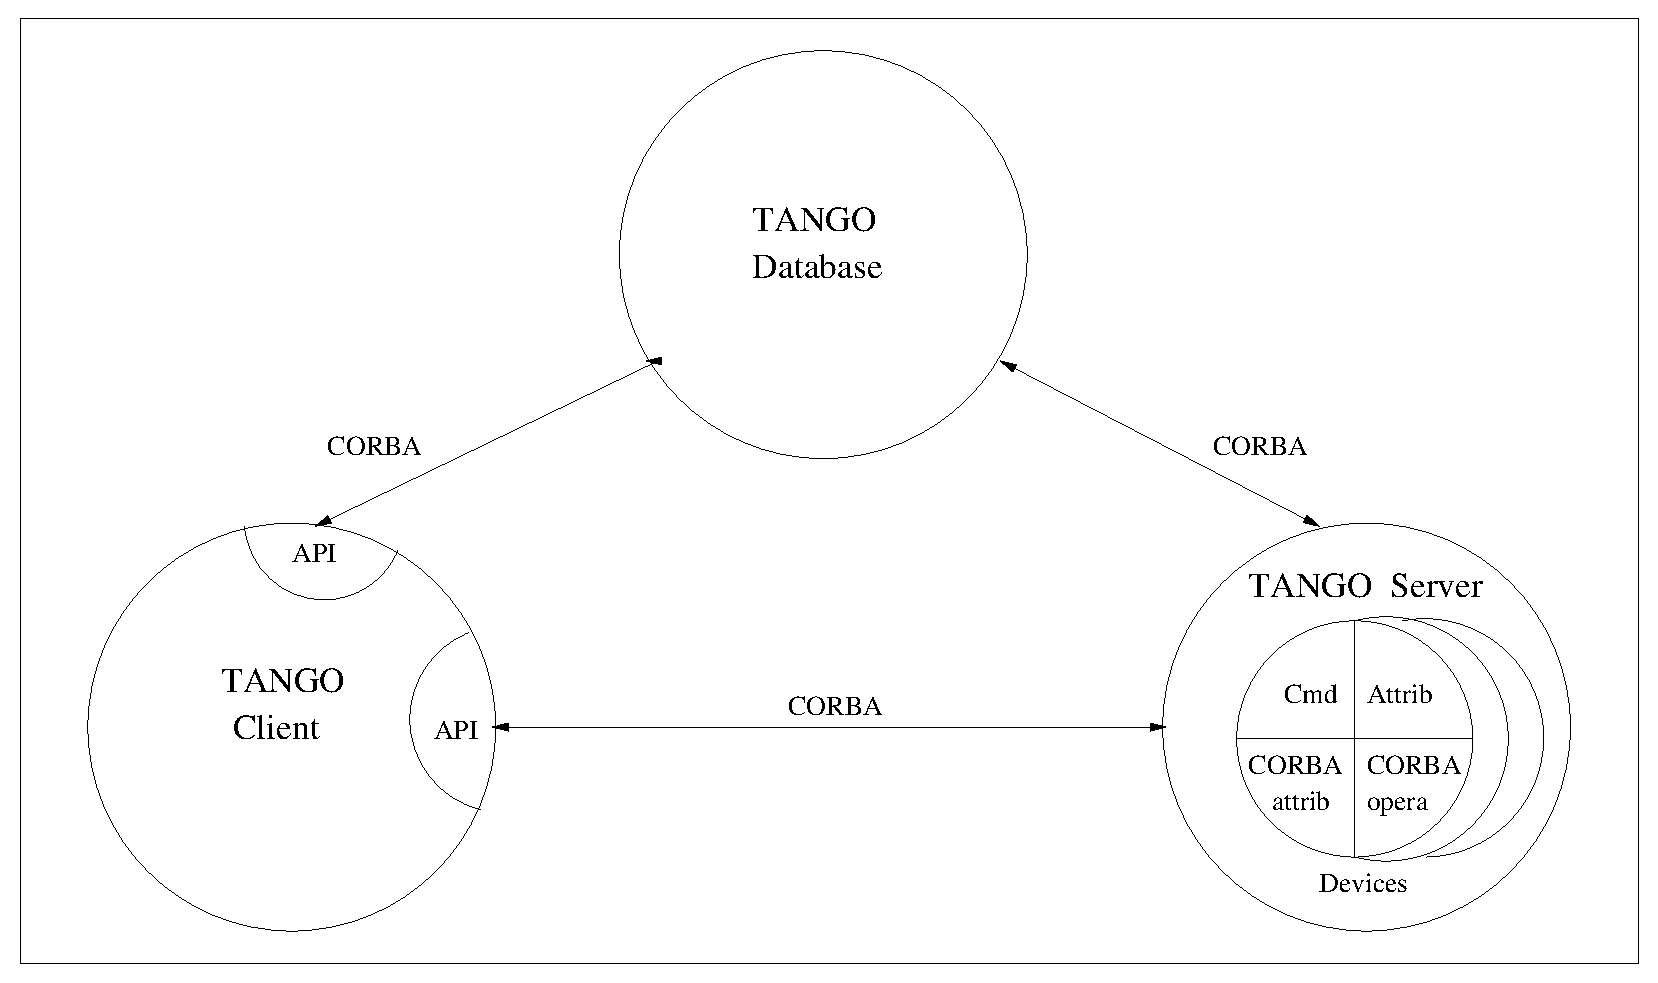
\includegraphics[width=12cm,height=7cm]{ds_model/archi}
\par\end{center}

\vspace{0.3cm}


The database is used during server and client startup phase to establish
connection between client and server.


\subsection{Communication between client and server using the API}

With the API, it is possible to request command to be executed on
a device or to read/write device attribute(s) using one of the two
communication models implemented. These two models are:
\begin{enumerate}
\item The synchronous model where client waits (and is blocked) for the
server to send the answer or until the timeout is reached
\item The asynchronous model. In this model, the clients send the request
and immediately returns. It is not blocked. It is free to do whatever
it has to do like updating a graphical user interface. The client
has the choice to retrieve the server answer by checking if the reply
is arrived by calling an API specific call or by requesting that a
call-back method is executed when the client receives the server answer.
\end{enumerate}
The asynchronous model is available with Tango release 3 and above.


\subsection{Tango events}

On top of the two communication model previously described, TANGO
offers an \textquotedbl{}event system\textquotedbl{}\index{event}.
The standard TANGO communication paradigm is a synchronou/asynchronous
two-way call. In this paradigm the call is initiated by the client
who contacts the server. The server handles the client's request and
sends the answer to the client or throws an exception which the client
catches. This paradigm involves two calls to receive a single answer
and requires the client to be active in initiating the request. If
the client has a permanent interest in a value he is obliged to poll
the server for an update in a value every time. This is not efficient
in terms of network bandwidth nor in terms of client programming.

For clients who are permanently interested in values the event-driven
communication paradigm is a more efficient and natural way of programming.
In this paradigm the client registers his interest once in an event
(value). After that the server informs the client every time the event
has occurred. This paradigm avoids the client polling, frees it for
doing other things, is fast and makes efficient use of the network.

Before TANGO release 8, TANGO used the CORBA OMG COS Notification
Service\index{Notification Service} to generates events. TANGO uses
the omniNotify\index{omniNotify} implementation of the Notification
service. omniNotify was developed in conjunction with the omniORB
CORBA implementation also used by TANGO. The heart of the Notification
Service is the notification daemon. The omniNotify daemons are the
processes which receive events from device servers and distribute
them to all clients which are subscribed. In order to distribute the
load of the events there is one notification daemon per host. Servers
send their events to the daemon on the local host. Clients and servers
get the IOR for the host from the TANGO database. 

The following figure is a schematic of the Tango event system for
Tango releases before Tango 8.

\vspace{0.3cm}


\begin{center}
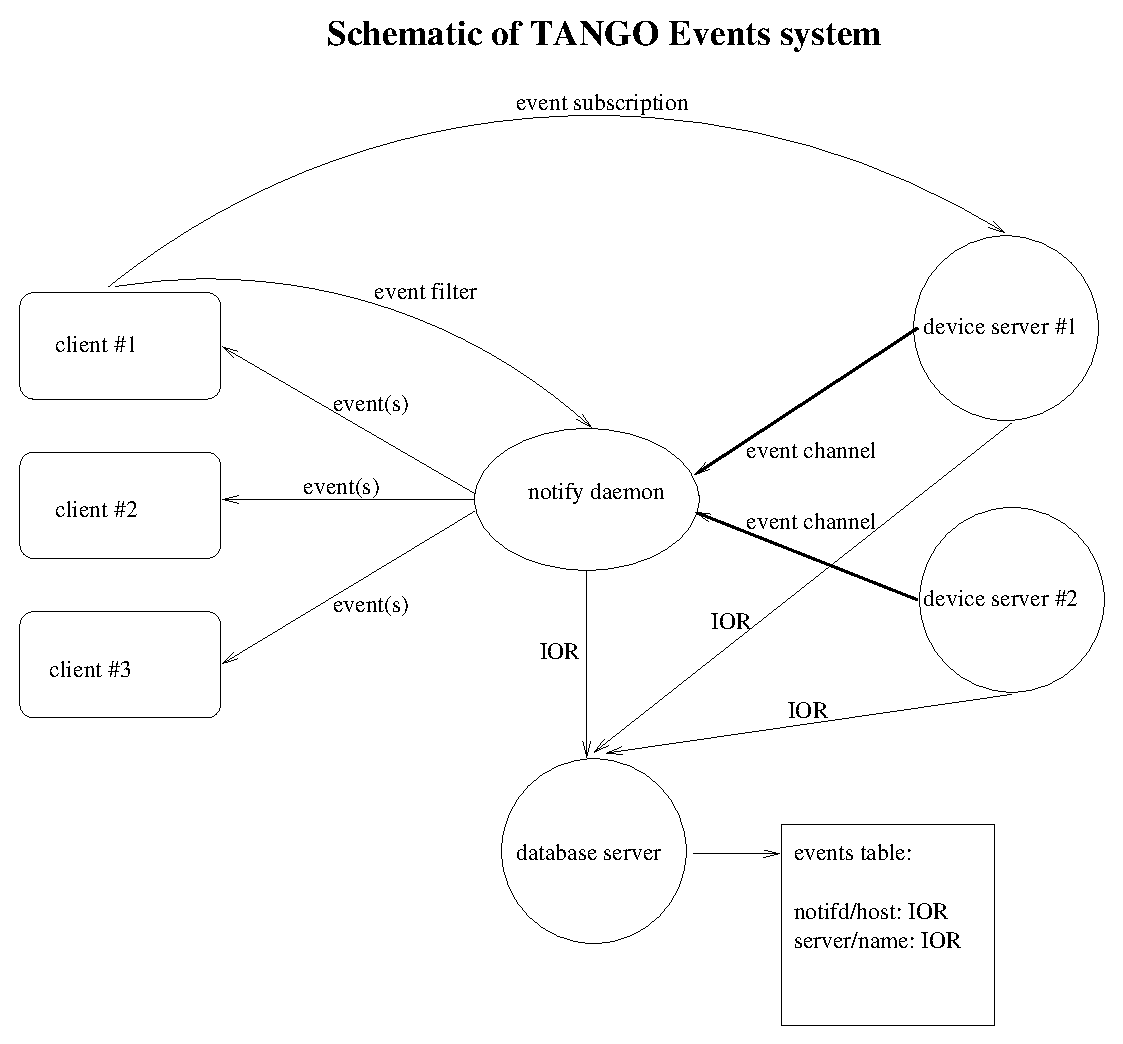
\includegraphics[bb=0bp 0bp 523bp 485bp,clip,scale=0.8]{ds_model/event_schematic}
\par\end{center}

\vspace{0.3cm}


Starting with Tango 8, a new design of the event system has been implemented.
This new design is based on the ZMQ\index{ZMQ} library. ZMQ is a
library allowing users to create communicating system. It implements
several well known communication pattern including the Publish/Subscribe\index{Publish/Subscribe}
pattern which is the basic of the new Tango event system. Using this
library, a separate notification service is not needed anymore and
event communiction is available with only client and server processes
which simplifies the overall design. Starting with Tango 8.1, the
event propagation between devices and clients could be done using
a multicasting\index{multicasting} protocol. The aim of this is to
reduce both the network bandwidth use and the CPU consumption on the
device server side. See chapter on Advanced Features to get all the
details on this feature.

The following figure is a schematic of the Tango event system for
Tango releases starting with Tango release 8.

\vspace{0.3cm}


\begin{center}
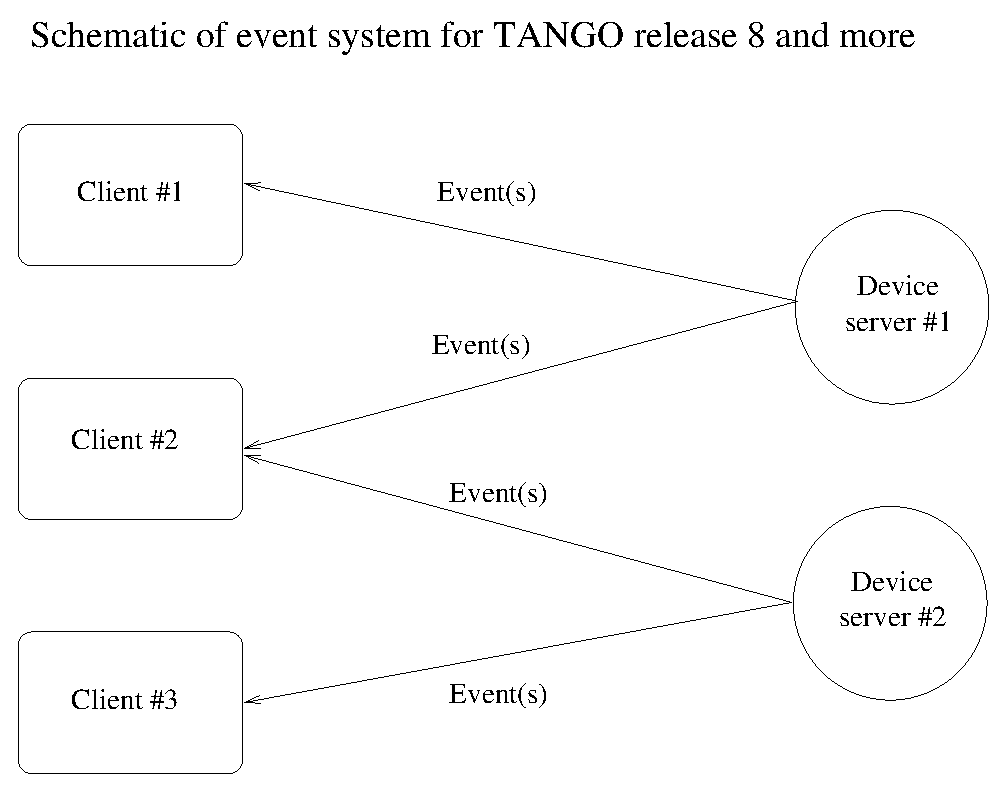
\includegraphics[bb=0bp 0bp 523bp 485bp,clip,scale=0.8]{ds_model/event_schematic_zmq}
\par\end{center}

\vspace{0.3cm}


\begin{center}

\vspace{5cm}


\label{OneRicardo}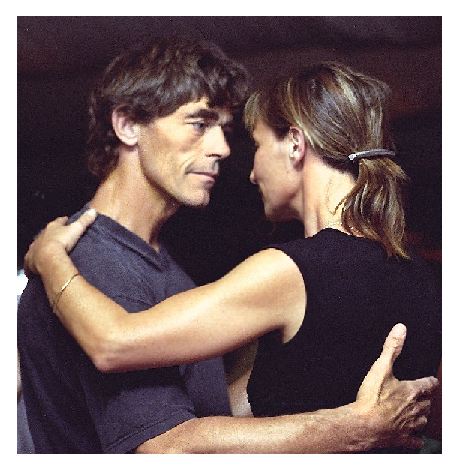
\includegraphics[scale=1.5]{dance/Eltaita-reduc}

\end{center}


\begin{comment}
The Tango API generalities 
\end{comment}


\chapter{Writing a TANGO client using TANGO APIs}


\section{Introduction}

\noindent TANGO devices and database are implemented using the TANGO
device server model. To access them the user has the CORBA interface
e.g. command\_inout(), write\_attributes() etc. defined by the idl
file. These methods are very low-level and assume a good working knowledge
of CORBA. In order to simplify this access, high-level api has been
implemented which hides all CORBA aspects of TANGO. In addition the
api hides details like how to connect to a device via the database,
how to reconnect after a device has been restarted, how to correctly
pack and unpack attributes and so on by implementing these in a manner
transparent to the user. The api provides a unified error handling
for all TANGO and CORBA errors. Unlike the CORBA C++ bindings the
TANGO api supports native C++ data types e.g. strings and vectors.

This chapter describes how to use these API's. It is not a reference
guide. Reference documentation is available as Web pages in the \href{http://www.tango-controls.org}{Tango Web site}


\section{\noindent Getting Started}

Refer to the chapter \textquotedbl{}Getting Started\textquotedbl{}
for an example on getting start with the C++ or Java api.


\section{\noindent Basic Philosophy}

\noindent The basic philosophy is to have high level classes to deal
with Tango devices. To communicate with Tango device, uses the \textbf{DeviceProxy\index{DeviceProxy}}
class. To send/receive data to/from Tango device, uses the \textbf{DeviceData\index{DeviceData},
DeviceAttribute\index{DeviceAttribute}} or \textbf{DevicePipe}\index{DevicePipe}
classes. To communicate with a group of devices, use the \textbf{Group\index{Group}}
class. If you are interested only in some attributes provided by a
Tango device, uses the \textbf{AttributeProxy\index{AttributeProxy}}
class. Even if the Tango database is implemented as any other devices
(and therefore accessible with one instance of a DeviceProxy class),
specific high level classes have been developped to query it. Uses
the \textbf{Database}\index{Database}, \textbf{DbDevice}\index{DbDevice},
\textbf{DbClass}\index{DbClass}, \textbf{DbServer\index{DbServer}}
or \textbf{DbData\index{DbData}} classes when interfacing the Tango
database. Callback for asynchronous requests or events are implemented
via a \textbf{CallBack\index{CallBack}} class. An utility class called
\textbf{ApiUtil\index{ApiUtil}} is also available.


\section{Data types}

The definition of the basic data type you can transfert using Tango
is:

\vspace{0.3cm}


\begin{center}
\begin{longtable}{|c|c|}
\hline 
Tango type name & C++ equivalent type\tabularnewline
\hline 
\hline 
DevBoolean & boolean\tabularnewline
\hline 
DevShort & short\tabularnewline
\hline 
DevEnum & enumeration (only for attribute / See chapter on advanced features)\tabularnewline
\hline 
DevLong & int (always 32 bits data)\tabularnewline
\hline 
DevLong64 & long long on 32 bits chip or long on 64 bits chip\tabularnewline
 & always 64 bits data\tabularnewline
\hline 
DevFloat & float\tabularnewline
\hline 
DevDouble & double\tabularnewline
\hline 
DevString & char {*}\tabularnewline
\hline 
DevEncoded & structure with 2 fields: a string and an array of unsigned char\tabularnewline
\hline 
DevUChar & unsigned char\tabularnewline
\hline 
DevUShort & unsigned short\tabularnewline
\hline 
DevULong & unsigned int (always 32 bits data)\tabularnewline
\hline 
DevULong64 & unsigned long long on 32 bits chip or unsigned long on 64 bits chip\tabularnewline
 & always 64 bits data\tabularnewline
\hline 
DevState & Tango specific data type\tabularnewline
\hline 
\end{longtable}
\par\end{center}

\vspace{0.3cm}


Using commands, you are able to transfert all these data types, array
of these basic types and two other Tango specific data types called
DevVarLongStringArray and DevVarDoubleStringArray. See chapter \ref{Data exchange}
to get details about them. You are also able to create attributes
using any of these basic data types to transfer data between clients
and servers.


\section{Request model\label{sec:Request-model}}

For the most important API remote calls (command\_inout, read\_attribute(s)
and write\_attribute(s)), Tango supports two kind of requests which
are the synchronous model and the asynchronous model. Synchronous\index{synchronous}
model means that the client wait (and is blocked) for the server to
send an answer. Asynchronous\index{asynchronous} model means that
the client does not wait for the server to send an answer. The client
sends the request and immediately returns allowing the CPU to do anything
else (like updating a graphical user interface). Device pipe\index{pipe}
supports only the synchronous model. Within Tango, there are two ways
to retrieve the server answer when using asynchronous model. They
are:
\begin{enumerate}
\item The polling\index{polling} mode
\item The callback\index{callback} mode
\end{enumerate}
In polling mode, the client executes a specific call to check if the
answer is arrived. If this is not the case, an exception is thrown.
If the reply is there, it is returned to the caller and if the reply
was an exception, it is re-thrown. There are two calls to check if
the reply is arrived:
\begin{itemize}
\item Call which does not wait before the server answer is returned to the
caller.
\item Call which wait with timeout before returning the server answer to
the caller (or throw the exception) if the answer is not arrived.
\end{itemize}
In callback model, the caller must supply a callback method which
will be executed when the command returns. They are two sub-modes:
\begin{enumerate}
\item The pull\index{pull} callback mode
\item The push\index{push} callback mode
\end{enumerate}
In the pull callback\index{callback} mode, the callback is triggered
if the server answer is arrived when the client decide it by calling
a \emph{synchronization} method (The client pull-out the answer).
In push mode, the callback is executed as soon as the reply arrives
in a separate thread (The server pushes the answer to the client).


\subsection{Synchronous model}

Synchronous access to Tango device are provided using the \emph{DeviceProxy}
or \emph{AttributeProxy} class. For the \emph{DeviceProxy} class,
the main synchronous call methods are :
\begin{itemize}
\item \emph{command\_inout()} to execute a Tango device command
\item \emph{read\_attribute()} or \emph{read\_attributes()} to read a Tango
device attribute(s)
\item \emph{write\_attribute()} or \emph{write\_attributes()} to write a
Tango device attribute(s)
\item \emph{write\_read\_attribute()} or \emph{write\_read\_attributes()}
to write then read Tango device attribute(s)
\item \emph{read\_pipe()} to read a Tango device pipe
\item \emph{write\_pipe()} to write a Tango device pipe
\item \emph{write\_read\_pipe()} to write then read Tango device pipe
\end{itemize}
For commands, data are send/received to/from device using the \emph{DeviceData}
class. For attributes, data are send/received to/from device attribute
using the \emph{DeviceAttribute} class. For pipes, data are send/receive
to/from device pipe using the \emph{DevicePipe\index{DevicePipe}}
and \emph{DevicePipeBlob\index{DevicePipeBlob}} classes.

In some cases, only attributes provided by a Tango device are interesting
for the application. You can use the \emph{AttributeProxy} class.
Its main synchronous methods are :
\begin{itemize}
\item \emph{read()} to read the attribute value
\item \emph{write()} to write the attribute value
\item \emph{write\_read()} to write then read the attribute value
\end{itemize}
Data are transmitted using the \emph{DeviceAttribute} class.


\subsection{Asynchronous model}

Asynchronous access to Tango device are provided using \emph{DeviceProxy}
or \emph{AttributeProxy, CallBack} and \emph{ApiUtil} classes methods.
The main asynchronous call methods and used classes are :
\begin{itemize}
\item To execute a command on a device

\begin{itemize}
\item \emph{DeviceProxy::command\_inout\_asynch()} and \emph{DeviceProxy::command\_inout\_reply()}
in polling model.
\item \emph{DeviceProxy::command\_inout\_asynch()}, \emph{DeviceProxy::get\_asynch\_replies()}
and \emph{CallBack} class in callback pull model
\item \emph{DeviceProxy::command\_inout\_asynch()}, \emph{ApiUtil::set\_asynch\_cb\_sub\_model()}
and \emph{CallBack} class in callback push model
\end{itemize}
\item To read a device attribute 

\begin{itemize}
\item \emph{DeviceProxy::read\_attribute\_asynch()} and \emph{DeviceProxy::read\_attribute\_reply()}
in polling model
\item \emph{DeviceProxy::read\_attribute\_asynch()}, \emph{DeviceProxy::get\_asynch\_replies()}
and \emph{CallBack} class in callback pull model.
\item \emph{DeviceProxy::read\_attribute\_asynch()}, \emph{ApiUtil::set\_asynch\_cb\_sub\_model()}
and \emph{CallBack} class in callback push model
\end{itemize}
\item To write a device attribute

\begin{itemize}
\item \emph{DeviceProxy::write\_attribute\_asynch()} in polling model
\item \emph{DeviceProxy::write\_attribute\_asynch()} and \emph{CallBack}
class in callback pull model
\item \emph{DeviceProxy::write\_attribute\_asynch()}, \emph{ApiUtil::set\_asynch\_cb\_sub\_model()}
and \emph{CallBack} class in callback push model
\end{itemize}
\end{itemize}
For commands, data are send/received to/from device using the \emph{DeviceData}
class. For attributes, data are send/received to/from device attribute
using the \emph{DeviceAttribute} class. It is also possible to generate
asynchronous request(s) using the \emph{AttributeProxy\index{AttributeProxy}}
class following the same schema than above. Methods to use are :
\begin{itemize}
\item \emph{read\_asynch(}) and \emph{read\_reply()} to asynchronously read
the attribute value
\item \emph{write\_asynch()} and \emph{write\_reply()} to asynchronously
write the attribute value
\end{itemize}

\section{Events\index{event}}


\subsection{Introduction}

Events are a critical part of any distributed control system. Their
aim is to provide a communication mechanism which is fast and efficient. 

The standard CORBA communication paradigm is a synchronous or asynchronous
two-way call. In this paradigm the call is initiated by the client
who contacts the server. The server handles the client's request and
sends the answer to the client or throws an exception which the client
catches. This paradigm involves two calls to receive a single answer
and requires the client to be active in initiating the request. If
the client has a permanent interest in a value he is obliged to poll
the server for an update in a value every time. This is not efficient
in terms of network bandwidth nor in terms of client programming.

For clients who are permanently interested in values the event-driven
communication paradigm is a more efficient and natural way of programming.
In this paradigm the client registers her interest once in an event
(value). After that the server informs the client every time the event
has occurred. This paradigm avoids the client polling, frees it for
doing other things, is fast and makes efficient use of the network.

The rest of this chapter explains how the TANGO events are implemented
and the application programmer's interface.


\subsection{Event definition}

TANGO events represent an alternative channel for reading TANGO device
attributes\index{attribute}. Device attributes values are sent to
all subscribed clients when an event occurs. Events can be an attribute
value change, a change in the data quality or a periodically send
event. The clients continue receiving events as long as they stay
subscribed. Most of the time, the device server polling thread detects
the event and then pushes the device attribute value to all clients.
Nevertheless, in some cases, the delay introduced by the polling thread
in the event propagation is detrimental. For such cases, some API
calls directly push the event. Until TANGO release 8, the omniNotify\index{omniNotify}
implementation of the CORBA Notification service\index{Notification Service}
was used to dispatch events. Starting with TANGO 8, this CORBA Notification
service has been replaced by the ZMQ\index{ZMQ} library which implements
a Publish/Subscribe communication model well adapted to TANGO events
communication.


\subsection{Event types}

The following eight event types have been implemented in TANGO :
\begin{enumerate}
\item \textbf{change\index{change}} - an event is triggered and the attribute
value is sent when the attribute value changes significantly. The
exact meaning of significant is device attribute dependent. For analog
and digital values this is a delta fixed per attribute, for string
values this is any non-zero change i.e. if the new attribute value
is not equal to the previous attribute value. The delta can either
be specified as a relative or absolute change. The delta is the same
for all clients unless a filter is specified (see below). To easily
write applications using the change event, it is also triggered in
the following case :

\begin{enumerate}
\item When a spectrum or image attribute size changes.
\item At event subscription time
\item When the polling thread receives an exception during attribute reading
\item When the polling thread detects that the attribute quality factor
has changed.
\item The first good reading of the attribute after the polling thread has
received exception when trying to read the attribute
\item The first time the polling thread detects that the attribute quality
factor has changed from INVALID to something else
\item When a change event is pushed manually from the device server code.
(\emph{DeviceImpl::push\_change\_event()}).
\item By the methods Attribute::set\_quality() and Attribute::set\_value\_date\_quality()
if a client has subscribed to the change event on the attribute. This
has been implemented for cases where the delay introduced by the polling
thread in the event propagation is not authorized.
\end{enumerate}
\item \textbf{periodic\index{periodic}} - an event is sent at a fixed periodic
interval. The frequency of this event is determined by the \emph{event\_period}
property of the attribute and the polling frequency. The polling frequency
determines the highest frequency at which the attribute is read. The
event\_period determines the highest frequency at which the periodic
event is sent. Note if the event\_period is not an integral number
of the polling period there will be a beating of the two frequencies%
\footnote{note: the polling is not synchronized is currently not synchronized
on the hour%
}. Clients can reduce the frequency at which they receive periodic
events by specifying a filter on the periodic event counter. 
\item \textbf{archive\index{archive}} - an event is sent if one of the
archiving conditions is satisfied. Archiving conditions are defined
via properties in the database. These can be a mixture of delta\_change
and periodic. Archive events can be send from the polling thread or
can be manually pushed from the device server code (\emph{DeviceImpl::push\_archive\_event()}).
\item \textbf{attribute configuration} - an event is sent if the attribute
configuration is changed.
\item \textbf{data ready} - This event is sent when coded by the device
server programmer who uses a specific method of one of the Tango device
server class to fire the event (\emph{DeviceImpl::push\_data\_ready\_event()}).
The rule of this event is to inform a client that it is now possible
to read an attribute. This could be useful in case of attribute with
many data.
\item \textbf{user} - The criteria and configuration of these user events
are managed by the device server programmer who uses a specific method
of one of the Tango device server class to fire the event (\emph{DeviceImpl::push\_event()}).
\item \textbf{device interface change} - This event is sent when the device
interface changes. Using Tango, it is possible to dynamically add/remove
attribute/command to a device. This event is the way to inform client(s)
that attribute/command has been added/removed from a device. Note
that this type of event is attached to a device and not to one attribute
(like all other event types). This event is triggered in the following
case :

\begin{enumerate}
\item A dynamic attribute or command is added or removed. The event is sent
after a small delay (50 mS) in order to eliminate the risk of events
storm in case several attributes/commands are added/removed in a loop 
\item At the end of admin device RestartServer or DevRestart command
\item After a re-connection due to a device server restart. Because the
device interface is not memorized, the event is sent even if it is
highly possible that the device interface has not changed. A flag
in the data propagated with the event inform listening applications
that the device interface change is not guaranteed. 
\item At event re-connection time. This case is similar to the previous
one (device interface change not guaranteed)
\end{enumerate}
\item \textbf{pipe} - This is the kind of event which has to be used when
the user want to push data through a pipe. This kind of event is only
sent by the user code by using a specific method (\emph{DeviceImpl::push\_pipe\_event()}).
There is no way to ask the Tango kernel to automatically push this
kind of event.
\end{enumerate}
The first three above events are automatically generated by the TANGO
library or fired by the user code. Events number 4 and 7 are only
automatically sent by the library and events 5, 6 and 8 are fired
only by the user code.


\subsection{Event filtering (Removed in Tango release 8 and above)}

Please, note that this feature is available only for Tango releases
older than Tango 8. The CORBA Notification Service allows event filtering.
This means that a client can ask the Notification Service to send
the event only if some filter is evaluated to true. Within the Tango
control system, some pre-defined fields can be used as filter. These
fields depend on the event type.

\vspace{0.3cm}


\begin{center}
\begin{longtable}{|c|c|c|c|}
\hline 
Event type & Filterable field name & Filterable field value & type\tabularnewline
\hline 
\hline 
 & delta\_change\_rel & Relative change (in \%) since last event & double\tabularnewline
\cline{2-4} 
\multicolumn{1}{|c|}{} & delta\_change\_abs & Absolute change since last event & double\tabularnewline
\cline{2-4} 
\multicolumn{1}{|c|}{change} & quality & Is set to 1 when the attribute quality factor has & double\tabularnewline
\multicolumn{1}{|c|}{} &  & changed, otherwise it is 0 & \tabularnewline
\cline{2-4} 
\multicolumn{1}{|c|}{} & forced\_event & Is set to 1 when the event was fired on exception  & double\tabularnewline
\multicolumn{1}{|c|}{} &  & or a quality factor set to invalid & \tabularnewline
\hline 
periodic & counter & Incremented each time the event is sent & long\tabularnewline
\hline 
\multicolumn{1}{|c|}{} & delta\_change\_rel & Relative change (in \%) since last event & double\tabularnewline
\cline{2-4} 
\multicolumn{1}{|c|}{} & delta\_change\_abs & Absolute change since last event & double\tabularnewline
\cline{2-4} 
 & quality & Is set to 1 when the attribute quality factor has & double\tabularnewline
 &  & changed, otherwise it is 0 & \tabularnewline
\cline{2-4} 
\multicolumn{1}{|c|}{archive} &  & Incremented each time the event is sent & \tabularnewline
\multicolumn{1}{|c|}{} & counter & for periodic reason. Set to -1 if event & long\tabularnewline
\multicolumn{1}{|c|}{} &  & sent for change reason & \tabularnewline
\cline{2-4} 
\multicolumn{1}{|c|}{} & forced\_event & Is set to 1 when the event was fired on exception & double\tabularnewline
\multicolumn{1}{|c|}{} &  & or a quality factor set to invalid & \tabularnewline
\cline{2-4} 
 & delta\_event & Number of milli-seconds since previous event & double\tabularnewline
\hline 
\end{longtable}
\par\end{center}

\vspace{0.3cm}


Filter are defined as a string following a grammar defined by CORBA.
It is defined in \cite{Notif_doc}. The following example shows you
the most common use of these filters in the Tango world :
\begin{itemize}
\item To receive periodic event one out of every three, the filter must
be \begin{center}\textquotedbl{}\$counter \% 3 == 0\textquotedbl{}\end{center}
\item To receive change event only if the relative change is greater than
20 \% (positive and negative), the filter must be \begin{center}\textquotedbl{}\$delta\_change\_rel
>= 20 or \$delta\_change\_rel <= -20\textquotedbl{}\end{center}
\item To receive a change event only on quality change, the filter must
be \begin{center}\textquotedbl{}\$quality == 1\textquotedbl{}\end{center}
\end{itemize}
For user events, the filter field name(s) and their value are defined
by the device server programmer.


\subsection{Application Programmer's Interface}

How to setup and use the TANGO events ? The interfaces described here
are intended as user friendly interfaces to the underlying CORBA calls.
The interface is modeled after the asynchronous\index{asynchronous}
\emph{command\_inout()\index{command-inout()}} interface so as to
maintain coherency. The event system supports \textbf{push callback
model} as well as the \textbf{pull callback model.}

The two event reception modes are:
\begin{itemize}
\item \textbf{Push callback model} : On event reception a callbacks method
gets immediately executed.
\item \textbf{Pull callback model} : The event will be buffered the client
until the client is ready to receive the event data. The client triggers
the execution of the callback method.
\end{itemize}
The event reception buffer in the \textbf{pull callback model}, is
implemented as a round robin buffer. The client can choose the size
when subscribing for the event. This way the client can set-up different
ways to receive events.
\begin{itemize}
\item Event reception buffer size = 1 : The client is interested only in
the value of the last event received. All other events that have been
received since the last reading are discarded.
\item Event reception buffer size > 1 : The client has chosen to keep an
event history of a given size. When more events arrive since the last
reading, older events will be discarded.
\item Event reception buffer size = ALL\_EVENTS : The client buffers all
received events. The buffer size is unlimited and only restricted
by the available memory for the client.
\end{itemize}

\subsubsection{Configuring events}

The attribute configuration set is used to configure under what conditions
events\index{event} are generated. A set of standard attribute properties
(part of the standard attribute configuration) are read from the database
at device startup time and used to configure the event engine. If
there are no properties defined then default values specified in the
code are used. 


\paragraph{change}

The attribute properties and their default values for the \textquotedbl{}change\textquotedbl{}
event are :
\begin{enumerate}
\item \textbf{rel\_change\index{rel-change}} - a property of maximum 2
values. It specifies the positive and negative relative change of
the attribute value w.r.t. the value of the previous change event
which will trigger the event. If the attribute is a spectrum or an
image then a change event is generated if any one of the attribute
value's satisfies the above criterium. If only one property is specified
then it is used for the positive and negative change. If no property
is specified, no events are generated.
\item \textbf{abs\_change\index{abs-change}} - a property of maximum 2
values.It specifies the positive and negative absolute change of the
attribute value w.r.t the value of the previous change event which
will trigger the event. If the attribute is a spectrum or an image
then a change event is generated if any one of the attribute value's
satisfies the above criterium. If only one property is specified then
it is used for the positive and negative change. If no properties
are specified then the relative change is used.
\end{enumerate}

\paragraph{periodic}

The attribute properties and their default values for the \textquotedbl{}periodic\textquotedbl{}
event are :
\begin{enumerate}
\item \textbf{event\_period\index{event-period}} - the minimum time between
events (in milliseconds). If no property is specified then a default
value of 1 second is used.
\end{enumerate}

\paragraph{archive}

The attribute properties and their default values for the \textquotedbl{}archive\textquotedbl{}
event are :
\begin{enumerate}
\item \textbf{archive\_rel\_change\index{archive-rel-change}} - a property
of maximum 2 values which specifies the positive and negative relative
change w.r.t. the previous attribute value which will trigger the
event. If the attribute is a spectrum or an image then an archive
event is generated if any one of the attribute value's satisfies the
above criterium. If only one property is specified then it is used
for the positive and negative change. If no properties are specified
then no events are generate.
\item \textbf{archive\_abs\_change\index{archive-abs-change}} - a property
of maximum 2 values which specifies the positive and negative absolute
change w.r.t the previous attribute value which will trigger the event.
If the attribute is a spectrum or an image then an archive event is
generated if any one of the attribute value's satisfies the above
criterium. If only one property is specified then it is used for the
positive and negative change. If no properties are specified then
the relative change is used.
\item \textbf{archive\_period\index{archive-period}} - the minimum time
between archive events (in milliseconds). If no property is specified,
no periodic archiving events are send.
\end{enumerate}

\subsubsection{C++ Clients}

This is the interface for clients who want to receive events\index{event}.
The main action of the client is to subscribe and unsubscribe to events.
Once the client has subscribed to one or more events the events are
received in a separate thread by the client.

Two reception modes are possible:
\begin{itemize}
\item On event reception a callbacks method gets immediately executed.
\item The event will be buffered until the client until the client is ready
to receive the event data.
\end{itemize}
The mode to be used has to be chosen when subscribing for the event.


\paragraph{Subscribing to events}

The client call to subscribe to an event is named \emph{DeviceProxy::subscribe\_event()\index{subscribe-event}}
. During the event subscription the client has to choose the event
reception mode to use. 

\textbf{Push model}:
\begin{lyxcode}
int~DeviceProxy::subscribe\_event(~

~~~~~~~~~~~~~const~string~\&attribute,~

~~~~~~~~~~~~~Tango::EventType~event,~

~~~~~~~~~~~~~Tango::CallBack~{*}callback,

~~~~~~~~~~~~~bool~stateless~=~false);
\end{lyxcode}
The client implements a callback method which is triggered when the
event is received. Note that this callback method will be executed
by a thread started by the underlying ORB. This thread is not the
application main thread. For Tango releases before 8, a similar call
with one extra parameter for event filtering is also available.

\textbf{Pull model}:
\begin{lyxcode}
int~DeviceProxy::subscribe\_event(~

~~~~~~~~~~~~~const~string~\&attribute,~

~~~~~~~~~~~~~Tango::EventType~event,~

~~~~~~~~~~~~~int~event\_queue\_size,

~~~~~~~~~~~~~bool~stateless~=~false);
\end{lyxcode}
The client chooses the size of the round robin event reception buffer.
Arriving events will be buffered until the client uses \emph{DeviceProxy::get\_events()\index{get-events}}
to extract the event data. For Tango releases before 8, a similar
call with one extra parameter for event filtering is also available.

On top of the user filter defined by the \emph{filters} parameter,
basic filtering is done based on the reason specified and the event
type. For example when reading the state and the reason specified
is \textquotedbl{}change\textquotedbl{} the event will be fired only
when the state changes. Events consist of an attribute name and the
event reason. A standard set of reasons are implemented by the system,
additional device specific reasons can be implemented by device servers
programmers. 

The stateless flag = false indicates that the event subscription will
only succeed when the given attribute is known and available in the
Tango system. Setting stateless = true will make the subscription
succeed, even if an attribute of this name was never known. The real
event subscription will happen when the given attribute will be available
in the Tango system.

Note that in this model, the callback method will be executed by the
thread doing the \emph{DeviceProxy::get\_events()} call.


\paragraph{The CallBack class}

In C++, the client has to implement a class inheriting from the Tango
CallBack\index{CallBack} class and pass this to the \emph{DeviceProxy::subscribe\_event()}
method. The CallBack class is the same class as the one proposed for
the TANGO asynchronous call. This is as follows for events :
\begin{lyxcode}
class~MyCallback~:~public~Tango::CallBack

\{

~~~.

~~~.

~~~.

~~~virtual~push\_event(Tango::EventData~{*});

~~~virtual~push\_event(Tango::AttrConfEventData~{*});

~~~virtual~push\_event(Tango::DataReadyEventData~{*});

~~~virtual~push\_event(Tango::DevIntrChangeEventData~{*});

~~~virtual~push\_event(Tango::PipeEventData~{*});

\}
\end{lyxcode}
where EventData\index{EventData} is defined as follows :
\begin{lyxcode}
class~EventData~

\{

~~~DeviceProxy~~~~~~~{*}device;

~~~string~~~~~~~~~~~~attr\_name;

~~~string~~~~~~~~~~~~event;

~~~DeviceAttribute~~~{*}attr\_value;

~~~bool~~~~~~~~~~~~~~err;

~~~DevErrorList~~~~~~errors;

\}
\end{lyxcode}
AttrConfEventData\index{AttrConfEventData} is defined as follows
:
\begin{lyxcode}
class~AttrConfEventData~

\{

~~~DeviceProxy~~~~~~~{*}device;

~~~string~~~~~~~~~~~~attr\_name;

~~~string~~~~~~~~~~~~event;

~~~AttributeInfoEx~~~{*}attr\_conf;

~~~bool~~~~~~~~~~~~~~err;

~~~DevErrorList~~~~~~errors;

\}
\end{lyxcode}
DataReadyEventData\index{DataReadyEventData} is defined as follows
:
\begin{lyxcode}
class~DataReadyEventData~

\{

~~~DeviceProxy~~~~~~~{*}device;

~~~string~~~~~~~~~~~~attr\_name;

~~~string~~~~~~~~~~~~event;

~~~int~~~~~~~~~~~~~~~attr\_data\_type;

~~~int~~~~~~~~~~~~~~~ctr;

~~~bool~~~~~~~~~~~~~~err;

~~~DevErrorList~~~~~~errors;

\}
\end{lyxcode}
DevIntrChangeEventData\index{DevIntrChangeEventData} is defined as
follows :
\begin{lyxcode}
class~DevIntrChangeEventData~

\{

~~~DeviceProxy~~~~~~~~~~~~device;

~~~string~~~~~~~~~~~~~~~~~event;

~~~string~~~~~~~~~~~~~~~~~device\_name;

~~~CommandInfoList~~~~~~~~cmd\_list;

~~~AttributeInfoListEx~~~~att\_list;

~~~bool~~~~~~~~~~~~~~~~~~~dev\_started;

~~~bool~~~~~~~~~~~~~~~~~~~err;

~~~DevErrorList~~~~~~~~~~~errors;

\}
\end{lyxcode}
and PipeEventData\index{PipeEventData} is defined as follows :
\begin{lyxcode}
class~PipeEventData~

\{

~~~DeviceProxy~~~~~~~{*}device;

~~~string~~~~~~~~~~~~pipe\_name;

~~~string~~~~~~~~~~~~event;

~~~DevicePipe~~~~~~~~{*}pipe\_value;

~~~bool~~~~~~~~~~~~~~err;

~~~DevErrorList~~~~~~errors;

\}
\end{lyxcode}
In push model, there are some cases (same callback used for events
coming from different devices hosted in device server process running
on different hosts) where the callback method could be executed concurently
by different threads started by the ORB. The user has to code his
callback method in a \textbf{thread}\index{thread} \textbf{safe}
manner.


\paragraph{Unsubscribing from an event }

Unsubscribe a client from receiving the event specified by \emph{event\_id}
is done by calling the \emph{DeviceProxy::unsubscribe\_event()\index{unsubscribe-event}}
method :
\begin{lyxcode}
void~DeviceProxy::unsubscribe\_event(int~event\_id);


\end{lyxcode}

\paragraph{Extract buffered event data}

When the pull model was chosen during the event subscription, the
received event data can be extracted with \emph{DeviceProxy::get\_events()\index{get-events}.}
Two possibilities are available for data extraction. Either a callback
method can be executed for every event in the buffer when using
\begin{lyxcode}
int~DeviceProxy::get\_events(~

~~~~~~~~~~~~~int~event\_id,~

~~~~~~~~~~~~~CallBack~{*}cb);
\end{lyxcode}
Or all the event data can be directly extracted as EventDataList\index{EventDataList},
AttrConfEventDataList\index{AttrConfEventDataList} , DataReadyEventDataList\index{DataReadyEventDataList},
DevIntrChangeEventDataList\index{DevIntrChangeEventDataList} or PipeEventDataList\index{PipeEventDataList}
when using
\begin{lyxcode}
int~DeviceProxy::get\_events(~

~~~~~~~~~~~~~int~event\_id,~

~~~~~~~~~~~~~EventDataList~\&event\_list);



int~DeviceProxy::get\_events(~

~~~~~~~~~~~~~int~event\_id,~

~~~~~~~~~~~~~AttrConfEventDataList~\&event\_list);



int~DeviceProxy::get\_events(~

~~~~~~~~~~~~~int~event\_id,~

~~~~~~~~~~~~~DataReadyEventDataList~\&event\_list);



int~DeviceProxy::get\_events(~

~~~~~~~~~~~~~int~event\_id,~

~~~~~~~~~~~~~DevIntrChangeEventDataList~\&event\_list);



int~DeviceProxy::get\_events(~

~~~~~~~~~~~~~int~event\_id,~

~~~~~~~~~~~~~PipeEventDataList~\&event\_list);
\end{lyxcode}
The event data lists are vectors of EventData, AttrConfEventData,
DataReadyEventData or PipeEventData pointers with special destructor
and clean-up methods to ease the memory handling.
\begin{lyxcode}
class~EventDataList:public~vector<EventData~{*}>

class~AttrConfEventDataList:public~vector<AttrConfEventData~{*}>

class~DataReadyEventDataList:public~vector<DataReadyEventData~{*}>

class~DevIntrChangeEventDataList:public~vector<DevIntrChangeEventData~{*}>

class~PipeEventDataList:public~vector<PipeEventData~{*}>
\end{lyxcode}

\paragraph{Example}

Here is a typical code example of a client to register and receive
events. First, you have to define a callback\index{CallBack} method
as follows:

%
% Copyright (C) :      2004,2005,2006,2007,2008,2009,2010,2011,2012,2013
%                      European Synchrotron Radiation Facility
%                      BP 220, Grenoble 38043
%                      FRANCE
%
% This file is part of Tango.
%
% Tango is free software: you can redistribute it and/or modify
% it under the terms of the GNU Lesser General Public License as published by
% the Free Software Foundation, either version 3 of the License, or
% (at your option) any later version.
%
% Tango is distributed in the hope that it will be useful,
% but WITHOUT ANY WARRANTY; without even the implied warranty of
% MERCHANTABILITY or FITNESS FOR A PARTICULAR PURPOSE.  See the
% GNU Lesser General Public License for more details.
%
% You should have received a copy of the GNU Lesser General Public License
% along with Tango.  If not, see <http://www.gnu.org/licenses/>.
%
\begin{flushleft}
\begin{picture}(0,0)
\thicklines
\put(0,0){\line(1,0){400}}
\end{picture}
\end{flushleft}

\begin{lyxcode}
class~DoubleEventCallBack~:~public~Tango::CallBack~

\{

~~~void~push\_event(Tango::EventData{*});

\};~

~



void~DoubleEventCallBack::push\_event(Tango::EventData~{*}myevent)

\{

~~~~Tango::DevVarDoubleArray~{*}double\_value;

~~~~try

~~~~\{

~~~~~~~~cout~<\textcompwordmark{}<~\textquotedbl{}DoubleEventCallBack::push\_event():~called~attribute~\textquotedbl{}~

~~~~~~~~~~~~~<\textcompwordmark{}<~myevent->attr\_name

~~~~~~~~~~~~~<\textcompwordmark{}<~\textquotedbl{}~event~\textquotedbl{}

~~~~~~~~~~~~~<\textcompwordmark{}<~myevent->event~

~~~~~~~~~~~~~<\textcompwordmark{}<~\textquotedbl{}~(err=\textquotedbl{}

~~~~~~~~~~~~~<\textcompwordmark{}<~myevent->err

~~~~~~~~~~~~~<\textcompwordmark{}<~\textquotedbl{})\textquotedbl{}~<\textcompwordmark{}<~endl;

~



~~~~~~~~~if~(!myevent->err)

~~~~~~~~~\{

~~~~~~~~~~~~~{*}(myevent->attr\_value)~>\textcompwordmark{}>~double\_value;

~~~~~~~~~~~~~cout~<\textcompwordmark{}<~\textquotedbl{}double~value~\textquotedbl{}

~~~~~~~~~~~~~~~~~~<\textcompwordmark{}<~({*}double\_value){[}0{]}

~~~~~~~~~~~~~~~~~~<\textcompwordmark{}<~endl;

~~~~~~~~~~~~~delete~double\_value;

~~~~~~~~~\}

~~~~\}

~~~~catch~(...)

~~~~\{

~~~~~~~~~cout~<\textcompwordmark{}<~\textquotedbl{}DoubleEventCallBack::push\_event():~could~not~extract~data~!\textbackslash{}n\textquotedbl{};

~~~~\}

\}
\end{lyxcode}
%
% Copyright (C) :      2004,2005,2006,2007,2008,2009,2010,2011,2012,2013
%                      European Synchrotron Radiation Facility
%                      BP 220, Grenoble 38043
%                      FRANCE
%
% This file is part of Tango.
%
% Tango is free software: you can redistribute it and/or modify
% it under the terms of the GNU Lesser General Public License as published by
% the Free Software Foundation, either version 3 of the License, or
% (at your option) any later version.
%
% Tango is distributed in the hope that it will be useful,
% but WITHOUT ANY WARRANTY; without even the implied warranty of
% MERCHANTABILITY or FITNESS FOR A PARTICULAR PURPOSE.  See the
% GNU Lesser General Public License for more details.
%
% You should have received a copy of the GNU Lesser General Public License
% along with Tango.  If not, see <http://www.gnu.org/licenses/>.
%
\begin{flushleft}
\begin{picture}(0,0)
\thicklines
\put(0,0){\line(1,0){400}}
\end{picture}
\end{flushleft}


Then the main code must subscribe\index{evebt-subscribe} to the event
and choose the push or the pull model for event reception.

\textbf{Push model}:

%
% Copyright (C) :      2004,2005,2006,2007,2008,2009,2010,2011,2012,2013
%                      European Synchrotron Radiation Facility
%                      BP 220, Grenoble 38043
%                      FRANCE
%
% This file is part of Tango.
%
% Tango is free software: you can redistribute it and/or modify
% it under the terms of the GNU Lesser General Public License as published by
% the Free Software Foundation, either version 3 of the License, or
% (at your option) any later version.
%
% Tango is distributed in the hope that it will be useful,
% but WITHOUT ANY WARRANTY; without even the implied warranty of
% MERCHANTABILITY or FITNESS FOR A PARTICULAR PURPOSE.  See the
% GNU Lesser General Public License for more details.
%
% You should have received a copy of the GNU Lesser General Public License
% along with Tango.  If not, see <http://www.gnu.org/licenses/>.
%
\begin{flushleft}
\begin{picture}(0,0)
\thicklines
\put(0,0){\line(1,0){400}}
\end{picture}
\end{flushleft}

\begin{lyxcode}
DoubleEventCallBack~{*}double\_callback~=~new~DoubleEventCallBack;~

~~~~~~

Tango::DeviceProxy~{*}mydevice~=~new~Tango::DeviceProxy(\textquotedbl{}my/device/1\textquotedbl{});

~

int~event\_id;

const~string~attr\_name(\textquotedbl{}current\textquotedbl{});

event\_id~=~mydevice->subscribe\_event(attr\_name,~

~~~~~~~~~~~~~~~~~~~~~~~~~Tango::CHANGE\_EVENT,

~~~~~~~~~~~~~~~~~~~~~~~~~double\_callback);

cout~<\textcompwordmark{}<~\textquotedbl{}event\_client()~id~=~\textquotedbl{}~<\textcompwordmark{}<~event\_id~<\textcompwordmark{}<~endl;



//~The~callback~methods~are~executed~by~the~Tango~event~reception~thread.

//~The~main~thread~is~not~concerned~of~event~reception.

//~Whatch~out~with~synchronisation~and~data~access~in~a~multi~threaded~environment!



sleep(1000);~//~wait~for~events

~

mydevice->unsubscribe\_event(event\_id);
\end{lyxcode}
%
% Copyright (C) :      2004,2005,2006,2007,2008,2009,2010,2011,2012,2013
%                      European Synchrotron Radiation Facility
%                      BP 220, Grenoble 38043
%                      FRANCE
%
% This file is part of Tango.
%
% Tango is free software: you can redistribute it and/or modify
% it under the terms of the GNU Lesser General Public License as published by
% the Free Software Foundation, either version 3 of the License, or
% (at your option) any later version.
%
% Tango is distributed in the hope that it will be useful,
% but WITHOUT ANY WARRANTY; without even the implied warranty of
% MERCHANTABILITY or FITNESS FOR A PARTICULAR PURPOSE.  See the
% GNU Lesser General Public License for more details.
%
% You should have received a copy of the GNU Lesser General Public License
% along with Tango.  If not, see <http://www.gnu.org/licenses/>.
%
\begin{flushleft}
\begin{picture}(0,0)
\thicklines
\put(0,0){\line(1,0){400}}
\end{picture}
\end{flushleft}


\textbf{Pull model}:

%
% Copyright (C) :      2004,2005,2006,2007,2008,2009,2010,2011,2012,2013
%                      European Synchrotron Radiation Facility
%                      BP 220, Grenoble 38043
%                      FRANCE
%
% This file is part of Tango.
%
% Tango is free software: you can redistribute it and/or modify
% it under the terms of the GNU Lesser General Public License as published by
% the Free Software Foundation, either version 3 of the License, or
% (at your option) any later version.
%
% Tango is distributed in the hope that it will be useful,
% but WITHOUT ANY WARRANTY; without even the implied warranty of
% MERCHANTABILITY or FITNESS FOR A PARTICULAR PURPOSE.  See the
% GNU Lesser General Public License for more details.
%
% You should have received a copy of the GNU Lesser General Public License
% along with Tango.  If not, see <http://www.gnu.org/licenses/>.
%
\begin{flushleft}
\begin{picture}(0,0)
\thicklines
\put(0,0){\line(1,0){400}}
\end{picture}
\end{flushleft}

\begin{lyxcode}
DoubleEventCallBack~{*}double\_callback~=~new~DoubleEventCallBack;

int~event\_queue\_size~=~100;~//~keep~the~last~100~events

~~~~~~

Tango::DeviceProxy~{*}mydevice~=~new~Tango::DeviceProxy(\textquotedbl{}my/device/1\textquotedbl{});

~

int~event\_id;

const~string~attr\_name(\textquotedbl{}current\textquotedbl{});

event\_id~=~mydevice->subscribe\_event(attr\_name,~

~~~~~~~~~~~~~~~~~~~~~~~~~Tango::CHANGE\_EVENT,

~~~~~~~~~~~~~~~~~~~~~~~~~event\_queue\_size);

cout~<\textcompwordmark{}<~\textquotedbl{}event\_client()~id~=~\textquotedbl{}~<\textcompwordmark{}<~event\_id~<\textcompwordmark{}<~endl;



//~Check~every~3~seconds~whether~new~events~have~arrived~and~trigger~the~callback~method~

//~for~the~new~events.



for~(int~i=0;~i~<~100;~i++)

\{

~~~~sleep~(3);~

~~~~

~~~~//~Read~the~stored~event~data~from~the~queue~and~call~the~callback~method~for~every~event.

~~~~mydevice->get\_events(event\_id,~double\_callback);

\}

~

event\_test->unsubscribe\_event(event\_id);
\end{lyxcode}
%
% Copyright (C) :      2004,2005,2006,2007,2008,2009,2010,2011,2012,2013
%                      European Synchrotron Radiation Facility
%                      BP 220, Grenoble 38043
%                      FRANCE
%
% This file is part of Tango.
%
% Tango is free software: you can redistribute it and/or modify
% it under the terms of the GNU Lesser General Public License as published by
% the Free Software Foundation, either version 3 of the License, or
% (at your option) any later version.
%
% Tango is distributed in the hope that it will be useful,
% but WITHOUT ANY WARRANTY; without even the implied warranty of
% MERCHANTABILITY or FITNESS FOR A PARTICULAR PURPOSE.  See the
% GNU Lesser General Public License for more details.
%
% You should have received a copy of the GNU Lesser General Public License
% along with Tango.  If not, see <http://www.gnu.org/licenses/>.
%
\begin{flushleft}
\begin{picture}(0,0)
\thicklines
\put(0,0){\line(1,0){400}}
\end{picture}
\end{flushleft}



\section{Group\index{group}}

A Tango Group provides the user with a single point of control for
a collection of devices. By analogy, one could see a Tango Group as
a proxy for a collection of devices. For instance, the Tango Group
API supplies a \emph{command\_inout()} method to execute the same
command on all the elements of a group. 

A Tango Group is also a hierarchical object. In other words, it is
possible to build a group of both groups and individual devices. This
feature allows creating logical views of the control system - each
view representing a hierarchical family of devices or a sub-system. 

In this chapter, we will use the term \emph{hierarchy} to refer to
a group and its sub-groups. The term \emph{Group} designates to the
local set of devices attached to a specific Group. 


\subsection{Getting started with Tango group}

The quickest way of getting started is to study an example\ldots{}

Imagine we are vacuum engineers who need to monitor and control hundreds
of gauges distributed over the 16 cells of a large-scale instrument.
Each cell contains several penning and pirani gauges. It also contains
one \textquotedbl{}strange\textquotedbl{} gauge. Our main requirement
is to be able to control the whole set of gauges, a family of gauges
located into a particular cell (e.g. all the penning gauges of the
6th cell) or a single gauge (e.g. the strange gauge of the 7th cell).
Using a Tango Group, such features are quite straightforward to obtain. 

Reading the description of the problem, the device hierarchy becomes
obvious. Our \textquotedbl{}gauges\textquotedbl{} group will have
the following structure: 
\begin{lyxcode}
->~gauges

~~|~~->~cell-01

~~|~~~~~|->~inst-c01/vac-gauge/strange~

~~|~~~~~|->~penning~

~~|~~~~~|~~~|->~inst-c01/vac-gauge/penning-01~

~~|~~~~~|~~~|->~inst-c01/vac-gauge/penning-02~

~~|~~~~~|~~~|-~...~

~~|~~~~~|~~~|->~inst-c01/vac-gauge/penning-xx~

~~|~~~~~|->~pirani~

~~|~~~~~~~~~|->~inst-c01/vac-gauge/pirani-01

~~|~~~~~~~~~|->~...~

~~|~~~~~~~~~|->~inst-c01/vac-gauge/pirani-xx~

~~|~~->~cell-02

~~|~~~~~|->~inst-c02/vac-gauge/strange~

~~|~~~~~|->~penning~

~~|~~~~~|~~~|->~inst-c02/vac-gauge/penning-01~

~~|~~~~~|~~~|->~...~

~~|~~~~~|~

~~|~~~~~|->~pirani~

~~|~~~~~|~~~|->~...~

~~|~~->~cell-03~

~~|~~~~~|->~...~

~~|~~~~~~~~~|~->~...~
\end{lyxcode}
In the C++, such a hierarchy can be build as follows (basic version): 

%
% Copyright (C) :      2004,2005,2006,2007,2008,2009,2010,2011,2012,2013
%                      European Synchrotron Radiation Facility
%                      BP 220, Grenoble 38043
%                      FRANCE
%
% This file is part of Tango.
%
% Tango is free software: you can redistribute it and/or modify
% it under the terms of the GNU Lesser General Public License as published by
% the Free Software Foundation, either version 3 of the License, or
% (at your option) any later version.
%
% Tango is distributed in the hope that it will be useful,
% but WITHOUT ANY WARRANTY; without even the implied warranty of
% MERCHANTABILITY or FITNESS FOR A PARTICULAR PURPOSE.  See the
% GNU Lesser General Public License for more details.
%
% You should have received a copy of the GNU Lesser General Public License
% along with Tango.  If not, see <http://www.gnu.org/licenses/>.
%
\begin{flushleft}
\begin{picture}(0,0)
\thicklines
\put(0,0){\line(1,0){400}}
\end{picture}
\end{flushleft}

\begin{lyxcode}
//-~step0:~create~the~root~group~

Tango::Group~{*}gauges~=~new~Tango::Group(\textquotedbl{}gauges\textquotedbl{});

~



//-~step1:~create~a~group~for~the~n-th~cell

Tango::Group~{*}cell~=~new~Tango::Group(\textquotedbl{}cell-01\textquotedbl{});

~



//-~step2:~make~the~cell~a~sub-group~of~the~root~group~

gauges->add(cell);

~



//-~step3:~create~a~\textquotedbl{}penning\textquotedbl{}~group~

Tango::Group~{*}gauge\_family~=~new~Tango::Group(\textquotedbl{}penning\textquotedbl{});

~



//-~step4:~add~all~penning~gauges~located~into~the~cell~(note~the~wildcard)

gauge\_family->add(\textquotedbl{}inst-c01/vac-gauge/penning{*}\textquotedbl{});

~



//-~step5:~add~the~penning~gauges~to~the~cell

cell->add(gauge\_family);

~



//-~step6:~create~a~\textquotedbl{}pirani\textquotedbl{}~group~

gauge\_family~=~new~Tango::Group(\textquotedbl{}pirani\textquotedbl{});

~



//-~step7:~add~all~pirani~gauges~located~into~the~cell~(note~the~wildcard)

gauge\_family->add(\textquotedbl{}inst-c01/vac-gauge/pirani{*}\textquotedbl{});

~



//-~step8:~add~the~pirani~gauges~to~the~cell

cell->add(gauge\_family);

~



//-~step9:~add~the~\textquotedbl{}strange\textquotedbl{}~gauge~to~the~cell

cell->add(\textquotedbl{}inst-c01/vac-gauge/strange\textquotedbl{});

~



//-~repeat~step~1~to~9~for~the~remaining~cells

cell~=~new~Tango::Group(\textquotedbl{}cell-02\textquotedbl{});

...
\end{lyxcode}
%
% Copyright (C) :      2004,2005,2006,2007,2008,2009,2010,2011,2012,2013
%                      European Synchrotron Radiation Facility
%                      BP 220, Grenoble 38043
%                      FRANCE
%
% This file is part of Tango.
%
% Tango is free software: you can redistribute it and/or modify
% it under the terms of the GNU Lesser General Public License as published by
% the Free Software Foundation, either version 3 of the License, or
% (at your option) any later version.
%
% Tango is distributed in the hope that it will be useful,
% but WITHOUT ANY WARRANTY; without even the implied warranty of
% MERCHANTABILITY or FITNESS FOR A PARTICULAR PURPOSE.  See the
% GNU Lesser General Public License for more details.
%
% You should have received a copy of the GNU Lesser General Public License
% along with Tango.  If not, see <http://www.gnu.org/licenses/>.
%
\begin{flushleft}
\begin{picture}(0,0)
\thicklines
\put(0,0){\line(1,0){400}}
\end{picture}
\end{flushleft}
 

\textbf{Important note}: There is no particular order to create the
hierarchy. However, the insertion order of the devices is conserved
throughout the lifecycle of the Group and cannot be changed. That
way, the Group implementation can guarantee the order in which results
are returned (see below). 

Keeping a reference to the root group\index{group} is enough to manage
the whole hierarchy (i.e. there no need to keep trace of the sub-groups
or individual devices). The Group interface provides methods to retrieve
a sub-group or an individual device. 

Be aware that a C++ group allways gets the ownership of its children
and deletes them when it is itself deleted. Therefore, never try to
delete a Group (respectively a DeviceProxy) returned by a call to
\emph{Tango::Group::get\_group()}\index{get-group} (respectively
to \emph{Tango::Group::get\_device()}\index{get-device}). Use the
\emph{Tango::Group::remove()}\index{remove} method instead (see the
Tango Group class API documentation for details). 

We can now perform any action on any element of our \textquotedbl{}gauges\textquotedbl{}
group. For instance, let's ping the whole hierarchy to be sure that
all devices are alive.

%
% Copyright (C) :      2004,2005,2006,2007,2008,2009,2010,2011,2012,2013
%                      European Synchrotron Radiation Facility
%                      BP 220, Grenoble 38043
%                      FRANCE
%
% This file is part of Tango.
%
% Tango is free software: you can redistribute it and/or modify
% it under the terms of the GNU Lesser General Public License as published by
% the Free Software Foundation, either version 3 of the License, or
% (at your option) any later version.
%
% Tango is distributed in the hope that it will be useful,
% but WITHOUT ANY WARRANTY; without even the implied warranty of
% MERCHANTABILITY or FITNESS FOR A PARTICULAR PURPOSE.  See the
% GNU Lesser General Public License for more details.
%
% You should have received a copy of the GNU Lesser General Public License
% along with Tango.  If not, see <http://www.gnu.org/licenses/>.
%
\begin{flushleft}
\begin{picture}(0,0)
\thicklines
\put(0,0){\line(1,0){400}}
\end{picture}
\end{flushleft}

\begin{lyxcode}
//-~ping~the~whole~hierarchy~

if~(gauges->ping()~==~true)

\{

~~~~std::cout~<\textcompwordmark{}<~\textquotedbl{}all~devices~alive\textquotedbl{}~<\textcompwordmark{}<~std::endl;

\}

else

\{

~~~~std::cout~<\textcompwordmark{}<~\textquotedbl{}at~least~one~dead/busy/locked/...~device\textquotedbl{}~<\textcompwordmark{}<~std::endl;

\}
\end{lyxcode}
%
% Copyright (C) :      2004,2005,2006,2007,2008,2009,2010,2011,2012,2013
%                      European Synchrotron Radiation Facility
%                      BP 220, Grenoble 38043
%                      FRANCE
%
% This file is part of Tango.
%
% Tango is free software: you can redistribute it and/or modify
% it under the terms of the GNU Lesser General Public License as published by
% the Free Software Foundation, either version 3 of the License, or
% (at your option) any later version.
%
% Tango is distributed in the hope that it will be useful,
% but WITHOUT ANY WARRANTY; without even the implied warranty of
% MERCHANTABILITY or FITNESS FOR A PARTICULAR PURPOSE.  See the
% GNU Lesser General Public License for more details.
%
% You should have received a copy of the GNU Lesser General Public License
% along with Tango.  If not, see <http://www.gnu.org/licenses/>.
%
\begin{flushleft}
\begin{picture}(0,0)
\thicklines
\put(0,0){\line(1,0){400}}
\end{picture}
\end{flushleft}
 


\subsection{Forward or not forward\index{forward}?}

Since a Tango Group is a hierarchical object, any action performed
on a group can be forwarded to its sub-groups. Most of the methods
in the Group interface have a so-called \emph{forward} option controlling
this propagation. When set to \emph{false}, the action is only performed
on the local set of devices. Otherwise, the action is also forwarded
to the sub-groups, in other words, propagated along the hierarchy.
In C++ , the forward option defaults to true (thanks to the C++ default
argument value). There is no such mechanism in Java and the forward
option must be systematically specified.


\subsection{Executing a command}

As a proxy for a collection of devices, the Tango Group provides an
interface similar to the DeviceProxy's. For the execution of a command,
the Group\index{group} interface contains several implementations
of the \emph{command\_inout\index{command-inout}} method. Both synchronous
and asynchronous forms are supported. 


\subsubsection{Obtaining command results\label{sub:Obt-cmd-results}}

Command results are returned using a Tango::GroupCmdReplyList\index{GroupCmdReplyList}.
This is nothing but a vector containing a Tango::GroupCmdReply\index{GroupCmdReply}
for each device in the group. The Tango::GroupCmdReply contains the
actual data (i.e. the Tango::DeviceData). By inheritance, it may also
contain any error occurred during the execution of the command (in
which case the data is invalid). 

We previously indicated that the Tango Group implementation guarantees
that the command results are returned in the order in which its elements
were attached to the group. For instance, if g1 is a group containing
three devices attached in the following order:
\begin{lyxcode}
g1->add(\textquotedbl{}my/device/01\textquotedbl{});

g1->add(\textquotedbl{}my/device/03\textquotedbl{});

g1->add(\textquotedbl{}my/device/02\textquotedbl{});
\end{lyxcode}
the results of 
\begin{lyxcode}
Tango::GroupCmdReplyList~crl~=~g1->command\_inout(\textquotedbl{}Status\textquotedbl{});
\end{lyxcode}
will be organized as follows:

\emph{crl{[}0{]}} contains the status of my/device/01 \\
\emph{crl{[}1{]}} contains the status of my/device/03 \\
\emph{crl{[}2{]}} contains the status of my/device/02

Things get more complicated if sub-groups are added \textquotedbl{}between\textquotedbl{}
devices.
\begin{lyxcode}
g2->add(\textquotedbl{}my/device/04\textquotedbl{});

g2->add(\textquotedbl{}my/device/05\textquotedbl{});

~



g4->add(\textquotedbl{}my/device/08\textquotedbl{});

g4->add(\textquotedbl{}my/device/09\textquotedbl{});

~



g3->add(\textquotedbl{}my/device/06\textquotedbl{});

g3->add(g4);

g3->add(\textquotedbl{}my/device/07\textquotedbl{});

~



g1->add(\textquotedbl{}my/device/01\textquotedbl{});

g1->add(g2);

g1->add(\textquotedbl{}my/device/03\textquotedbl{});

g1->add(g3);

g1->add(\textquotedbl{}my/device/02\textquotedbl{});
\end{lyxcode}
The result order in the Tango::GroupCmdReplyList depends on the value
of the forward\index{forward} option. If set to \emph{true}, the
results will be organized as follows:
\begin{lyxcode}
Tango::GroupCmdReplyList~crl~=~g1->command\_inout(\textquotedbl{}Status\textquotedbl{},~true);
\end{lyxcode}
\emph{crl{[}0{]}} contains the status of my/device/01 which belongs
to g1\\
\emph{crl{[}1{]}} contains the status of my/device/04 which belongs
to g1.g2\\
\emph{crl{[}2{]}} contains the status of my/device/05 which belongs
to g1.g2\\
\emph{crl{[}3{]}} contains the status of my/device/03 which belongs
to g1\\
\emph{crl{[}4{]}} contains the status of my/device/06 which belongs
to g1.g3\\
\emph{crl{[}5{]}} contains the status of my/device/08 which belongs
to g1.g3.g4\\
\emph{crl{[}6{]}} contains the status of my/device/09 which belongs
to g1.g3.g \\
\emph{crl{[}7{]}} contains the status of my/device/07 which belongs
to g1.g3\\
\emph{crl{[}8{]}} contains the status of my/device/02 which belongs
to g1 

If the forward option is set to \emph{false}, the results are:
\begin{lyxcode}
Tango::GroupCmdReplyList~crl~=~g1->command\_inout(\textquotedbl{}Status\textquotedbl{},~false);~
\end{lyxcode}
\emph{crl{[}0{]}} contains the status of my/device/01 which belongs
to g \\
\emph{crl{[}1{]}} contains the status of my/device/03 which belongs
to g1\\
\emph{crl{[}2{]}} contains the status of my/device/02 which belongs
to g1

The Tango::GroupCmdReply contains some public members allowing the
identification of both the device (Tango::GroupCmdReply::dev\_name\index{dev-name})
and the command (Tango::GroupCmdReply::obj\_name\index{obj-name}).
It means that, depending of your application, you can associate a
response with its source using its position in the response list or
using the Tango::GroupCmdReply::dev\_name member.


\subsubsection{Case 1: a command, no argument\label{sub:Case-1}}

As an example, we execute the Status command on the whole hierarchy
synchronously.
\begin{lyxcode}
Tango::GroupCmdReplyList~crl~=~gauges->command\_inout(\textquotedbl{}Status\textquotedbl{});
\end{lyxcode}
As a first step in the results processing, it could be interesting
to check value returned by the \emph{has\_failed\index{has-failed}()}
method of the GroupCmdReplyList\index{GroupCmdReplyList}. If it is
set to true, it means that at least one error occurred during the
execution of the command (i.e. at least one device gave error).

%
% Copyright (C) :      2004,2005,2006,2007,2008,2009,2010,2011,2012,2013
%                      European Synchrotron Radiation Facility
%                      BP 220, Grenoble 38043
%                      FRANCE
%
% This file is part of Tango.
%
% Tango is free software: you can redistribute it and/or modify
% it under the terms of the GNU Lesser General Public License as published by
% the Free Software Foundation, either version 3 of the License, or
% (at your option) any later version.
%
% Tango is distributed in the hope that it will be useful,
% but WITHOUT ANY WARRANTY; without even the implied warranty of
% MERCHANTABILITY or FITNESS FOR A PARTICULAR PURPOSE.  See the
% GNU Lesser General Public License for more details.
%
% You should have received a copy of the GNU Lesser General Public License
% along with Tango.  If not, see <http://www.gnu.org/licenses/>.
%
\begin{flushleft}
\begin{picture}(0,0)
\thicklines
\put(0,0){\line(1,0){400}}
\end{picture}
\end{flushleft}

\begin{lyxcode}
if~(crl.has\_failed())

\{

~~~~cout~<\textcompwordmark{}<~\textquotedbl{}at~least~one~error~occurred\textquotedbl{}~<\textcompwordmark{}<~endl;

\}

else

\{

~~~~cout~<\textcompwordmark{}<~\textquotedbl{}no~error~\textquotedbl{}~<\textcompwordmark{}<~endl;

\}
\end{lyxcode}
%
% Copyright (C) :      2004,2005,2006,2007,2008,2009,2010,2011,2012,2013
%                      European Synchrotron Radiation Facility
%                      BP 220, Grenoble 38043
%                      FRANCE
%
% This file is part of Tango.
%
% Tango is free software: you can redistribute it and/or modify
% it under the terms of the GNU Lesser General Public License as published by
% the Free Software Foundation, either version 3 of the License, or
% (at your option) any later version.
%
% Tango is distributed in the hope that it will be useful,
% but WITHOUT ANY WARRANTY; without even the implied warranty of
% MERCHANTABILITY or FITNESS FOR A PARTICULAR PURPOSE.  See the
% GNU Lesser General Public License for more details.
%
% You should have received a copy of the GNU Lesser General Public License
% along with Tango.  If not, see <http://www.gnu.org/licenses/>.
%
\begin{flushleft}
\begin{picture}(0,0)
\thicklines
\put(0,0){\line(1,0){400}}
\end{picture}
\end{flushleft}


Now, we have to process each \textquotedbl{}individual response\textquotedbl{}
in the list. 


\subsubsection{A few words on error handling and data extraction}

Depending of the application and/or the developer's programming habits,
each individual error can be handle by the C++ (or Java) exception\index{exception}
mechanism or using the dedicated \emph{has\_failed\index{has-failed}()}
method. The GroupReply\index{GroupReply} class - which is the mother
class of both GroupCmdReply\index{GroupCmdReply} and GroupAttrReply\index{GroupAttrReply}
- contains a static method to enable (or disable) exceptions called
\emph{enable\_exception()}\index{enable-exception()}. By default,
exceptions are disabled. The following example is proposed with both
exceptions enable and disable. 

In C++, data can be extracted directly from an individual reply. The
GroupCmdReply interface contains a template operator >\textcompwordmark{}>
allowing the extraction of any supported Tango type (in fact the actual
data extraction is delegated to DeviceData::operator >\textcompwordmark{}>).
One dedicated extract method is also provided in order to extract
DevVarLongStringArray and DevVarDoubleStringArray types to std::vectors.

Error and data handling C++ example:

%
% Copyright (C) :      2004,2005,2006,2007,2008,2009,2010,2011,2012,2013
%                      European Synchrotron Radiation Facility
%                      BP 220, Grenoble 38043
%                      FRANCE
%
% This file is part of Tango.
%
% Tango is free software: you can redistribute it and/or modify
% it under the terms of the GNU Lesser General Public License as published by
% the Free Software Foundation, either version 3 of the License, or
% (at your option) any later version.
%
% Tango is distributed in the hope that it will be useful,
% but WITHOUT ANY WARRANTY; without even the implied warranty of
% MERCHANTABILITY or FITNESS FOR A PARTICULAR PURPOSE.  See the
% GNU Lesser General Public License for more details.
%
% You should have received a copy of the GNU Lesser General Public License
% along with Tango.  If not, see <http://www.gnu.org/licenses/>.
%
\begin{flushleft}
\begin{picture}(0,0)
\thicklines
\put(0,0){\line(1,0){400}}
\end{picture}
\end{flushleft}

\begin{lyxcode}
//-{}-{}-{}-{}-{}-{}-{}-{}-{}-{}-{}-{}-{}-{}-{}-{}-{}-{}-{}-{}-{}-{}-{}-{}-{}-{}-{}-{}-{}-{}-{}-{}-{}-{}-{}-{}-{}-{}-{}-{}-{}-{}-{}-{}-{}-{}-{}-{}-{}-{}-{}-{}-{}-{}-

//-~synch.~group~command~example~with~exception~enabled

//-{}-{}-{}-{}-{}-{}-{}-{}-{}-{}-{}-{}-{}-{}-{}-{}-{}-{}-{}-{}-{}-{}-{}-{}-{}-{}-{}-{}-{}-{}-{}-{}-{}-{}-{}-{}-{}-{}-{}-{}-{}-{}-{}-{}-{}-{}-{}-{}-{}-{}-{}-{}-{}-{}-

//-~enable~exceptions~and~save~current~mode

bool~last\_mode~=~GroupReply::enable\_exception(true);

//-~process~each~response~in~the~list~...

for~(int~r~=~0;~r~<~crl.size();~r++)

\{

//-~enter~a~try/catch~block

~~~try

~~~\{

//-~try~to~extract~the~data~from~the~r-th~reply

//-~suppose~data~contains~a~double

~~~~~~~double~ans;

~~~~~~~crl{[}r{]}~>\textcompwordmark{}>~ans;

~~~~~~~cout~<\textcompwordmark{}<~crl{[}r{]}.dev\_name()

~~~~~~~~~~~~<\textcompwordmark{}<~\textquotedbl{}::\textquotedbl{}

~~~~~~~~~~~~<\textcompwordmark{}<~crl{[}r{]}.obj\_name()

~~~~~~~~~~~~<\textcompwordmark{}<~\textquotedbl{}~returned~\textquotedbl{}

~~~~~~~~~~~~<\textcompwordmark{}<~ans

~~~~~~~~~~~~<\textcompwordmark{}<~endl;

~~~~\}

~~~~catch~(const~DevFailed\&~df)

~~~~\{

//-~DevFailed~caught~while~trying~to~extract~the~data~from~reply

~~~~~~for~(int~err~=~0;~err~<~df.errors.length();~err++)

~~~~~~\{

~~~~~~~~~~~cout~<\textcompwordmark{}<~\textquotedbl{}error:~\textquotedbl{}~<\textcompwordmark{}<~df.errors{[}err{]}.desc.in()~<\textcompwordmark{}<~endl;

~~~~~~\}

//-~alternatively,~one~can~use~crl{[}r{]}.get\_err\_stack()~see~below

~~~~\}

~~~~catch~(...)

~~~~\{

~~~~~~~cout~<\textcompwordmark{}<~\textquotedbl{}unknown~exception~caught\textquotedbl{};

~~~~\}

\}

//-~restore~last~exception~mode~(if~needed)

GroupReply::enable\_exception(last\_mode);

//-~Clear~the~response~list~(if~reused~later~in~the~code)

crl.reset();

~



//-{}-{}-{}-{}-{}-{}-{}-{}-{}-{}-{}-{}-{}-{}-{}-{}-{}-{}-{}-{}-{}-{}-{}-{}-{}-{}-{}-{}-{}-{}-{}-{}-{}-{}-{}-{}-{}-{}-{}-{}-{}-{}-{}-{}-{}-{}-{}-{}-{}-{}-{}-{}-{}-{}-

//-~synch.~group~command~example~with~exception~disabled

//-{}-{}-{}-{}-{}-{}-{}-{}-{}-{}-{}-{}-{}-{}-{}-{}-{}-{}-{}-{}-{}-{}-{}-{}-{}-{}-{}-{}-{}-{}-{}-{}-{}-{}-{}-{}-{}-{}-{}-{}-{}-{}-{}-{}-{}-{}-{}-{}-{}-{}-{}-{}-{}-{}-

//-~disable~exceptions~and~save~current~mode~bool

last\_mode~=~GroupReply::enable\_exception(false);

//-~process~each~response~in~the~list~...

for~(int~r~=~0;~r~<~crl.size();~r++)

\{

//-~did~the~r-th~device~give~error?

~~~~if~(crl{[}r{]}.has\_failed()~==~true)

~~~~\{

//-~printout~error~description

~~~~~~~cout~<\textcompwordmark{}<~\textquotedbl{}an~error~occurred~while~executing~\textquotedbl{}

~~~~~~~~~~~~<\textcompwordmark{}<~crl{[}r{]}.obj\_name()

~~~~~~~~~~~~<\textcompwordmark{}<~\textquotedbl{}~on~\textquotedbl{}~

~~~~~~~~~~~~<\textcompwordmark{}<~crl{[}r{]}.dev\_name()~<\textcompwordmark{}<~endl;

//-~dump~error~stack

~~~~~~~const~DevErrorList\&~el~=~crl{[}r{]}.get\_err\_stack();

~~~~~~~for~(int~err~=~0;~err~<~el.size();~err++)

~~~~~~~\{

~~~~~~~~~~~cout~<\textcompwordmark{}<~el{[}err{]}.desc.in();

~~~~~~~\}

~~~~\}

~~~~else

~~~~\{

//-~no~error~(suppose~data~contains~a~double)

~~~~~~~double~ans;

~~~~~~~bool~result~=~crl{[}r{]}~>\textcompwordmark{}>~ans;

~~~~~~~if~(result~==~false)

~~~~~~~\{

~~~~~~~~~~~cout~<\textcompwordmark{}<~\textquotedbl{}could~not~extract~double~from~\textquotedbl{}

~~~~~~~~~~~~~~~~<\textcompwordmark{}<~crl{[}r{]}.dev\_name()

~~~~~~~~~~~~~~~~<\textcompwordmark{}<~\textquotedbl{}~reply\textquotedbl{}

~~~~~~~~~~~~~~~~<\textcompwordmark{}<~endl;

~~~~~~~\}

~~~~~~~else

~~~~~~~\{

~~~~~~~~~~~cout~<\textcompwordmark{}<~crl{[}r{]}.dev\_name()

~~~~~~~~~~~~~~~~<\textcompwordmark{}<~\textquotedbl{}::\textquotedbl{}

~~~~~~~~~~~~~~~~<\textcompwordmark{}<~crl{[}r{]}.obj\_name()

~~~~~~~~~~~~~~~~<\textcompwordmark{}<~\textquotedbl{}~returned~\textquotedbl{}

~~~~~~~~~~~~~~~~<\textcompwordmark{}<~ans

~~~~~~~~~~~~~~~~<\textcompwordmark{}<~endl;

~~~~~~~\}

~~~~\}

\}

//-~restore~last~exception~mode~(if~needed)

GroupReply::enable\_exception(last\_mode);

//-~Clear~the~response~list~(if~reused~later~in~the~code)

crl.reset();
\end{lyxcode}
%
% Copyright (C) :      2004,2005,2006,2007,2008,2009,2010,2011,2012,2013
%                      European Synchrotron Radiation Facility
%                      BP 220, Grenoble 38043
%                      FRANCE
%
% This file is part of Tango.
%
% Tango is free software: you can redistribute it and/or modify
% it under the terms of the GNU Lesser General Public License as published by
% the Free Software Foundation, either version 3 of the License, or
% (at your option) any later version.
%
% Tango is distributed in the hope that it will be useful,
% but WITHOUT ANY WARRANTY; without even the implied warranty of
% MERCHANTABILITY or FITNESS FOR A PARTICULAR PURPOSE.  See the
% GNU Lesser General Public License for more details.
%
% You should have received a copy of the GNU Lesser General Public License
% along with Tango.  If not, see <http://www.gnu.org/licenses/>.
%
\begin{flushleft}
\begin{picture}(0,0)
\thicklines
\put(0,0){\line(1,0){400}}
\end{picture}
\end{flushleft}


Now execute the same command asynchronously. C++ example:

%
% Copyright (C) :      2004,2005,2006,2007,2008,2009,2010,2011,2012,2013
%                      European Synchrotron Radiation Facility
%                      BP 220, Grenoble 38043
%                      FRANCE
%
% This file is part of Tango.
%
% Tango is free software: you can redistribute it and/or modify
% it under the terms of the GNU Lesser General Public License as published by
% the Free Software Foundation, either version 3 of the License, or
% (at your option) any later version.
%
% Tango is distributed in the hope that it will be useful,
% but WITHOUT ANY WARRANTY; without even the implied warranty of
% MERCHANTABILITY or FITNESS FOR A PARTICULAR PURPOSE.  See the
% GNU Lesser General Public License for more details.
%
% You should have received a copy of the GNU Lesser General Public License
% along with Tango.  If not, see <http://www.gnu.org/licenses/>.
%
\begin{flushleft}
\begin{picture}(0,0)
\thicklines
\put(0,0){\line(1,0){400}}
\end{picture}
\end{flushleft}

\begin{lyxcode}
//-{}-{}-{}-{}-{}-{}-{}-{}-{}-{}-{}-{}-{}-{}-{}-{}-{}-{}-{}-{}-{}-{}-{}-{}-{}-{}-{}-{}-{}-{}-{}-{}-{}-{}-{}-{}-{}-{}-{}-{}-{}-{}-{}-{}-{}-{}-{}-{}-{}-{}-{}-{}-{}-{}-

//-~asynch.~group~command~example~(C++~example)

//-{}-{}-{}-{}-{}-{}-{}-{}-{}-{}-{}-{}-{}-{}-{}-{}-{}-{}-{}-{}-{}-{}-{}-{}-{}-{}-{}-{}-{}-{}-{}-{}-{}-{}-{}-{}-{}-{}-{}-{}-{}-{}-{}-{}-{}-{}-{}-{}-{}-{}-{}-{}-{}-{}-

long~request\_id~=~gauges->command\_inout\_asynch(\textquotedbl{}Status\textquotedbl{});

//-~do~some~work

do\_some\_work();

~

~

//-~get~results

crl~=~gauges->command\_inout\_reply(request\_id);

//-~process~responses~as~previously~describe~in~the~synch.~implementation

for~(int~r~=~0;~r~<~crl.size();~r++)

\{

//-~data~processing~and~error~handling~goes~here

//-~copy/paste~code~from~previous~example

.~.~.

\}

//-~clear~the~response~list~(if~reused~later~in~the~code)

crl.reset();
\end{lyxcode}
%
% Copyright (C) :      2004,2005,2006,2007,2008,2009,2010,2011,2012,2013
%                      European Synchrotron Radiation Facility
%                      BP 220, Grenoble 38043
%                      FRANCE
%
% This file is part of Tango.
%
% Tango is free software: you can redistribute it and/or modify
% it under the terms of the GNU Lesser General Public License as published by
% the Free Software Foundation, either version 3 of the License, or
% (at your option) any later version.
%
% Tango is distributed in the hope that it will be useful,
% but WITHOUT ANY WARRANTY; without even the implied warranty of
% MERCHANTABILITY or FITNESS FOR A PARTICULAR PURPOSE.  See the
% GNU Lesser General Public License for more details.
%
% You should have received a copy of the GNU Lesser General Public License
% along with Tango.  If not, see <http://www.gnu.org/licenses/>.
%
\begin{flushleft}
\begin{picture}(0,0)
\thicklines
\put(0,0){\line(1,0){400}}
\end{picture}
\end{flushleft}



\subsubsection{Case 2: a command, one argument\label{sub:Case-2} }

Here, we give an example in which the same input argument is applied
to all devices in the group (or its sub-groups). 

In C++:

%
% Copyright (C) :      2004,2005,2006,2007,2008,2009,2010,2011,2012,2013
%                      European Synchrotron Radiation Facility
%                      BP 220, Grenoble 38043
%                      FRANCE
%
% This file is part of Tango.
%
% Tango is free software: you can redistribute it and/or modify
% it under the terms of the GNU Lesser General Public License as published by
% the Free Software Foundation, either version 3 of the License, or
% (at your option) any later version.
%
% Tango is distributed in the hope that it will be useful,
% but WITHOUT ANY WARRANTY; without even the implied warranty of
% MERCHANTABILITY or FITNESS FOR A PARTICULAR PURPOSE.  See the
% GNU Lesser General Public License for more details.
%
% You should have received a copy of the GNU Lesser General Public License
% along with Tango.  If not, see <http://www.gnu.org/licenses/>.
%
\begin{flushleft}
\begin{picture}(0,0)
\thicklines
\put(0,0){\line(1,0){400}}
\end{picture}
\end{flushleft}

\begin{lyxcode}
//-~the~argument~value

double~d~=~0.1;

//-~insert~it~into~the~TANGO~generic~container~for~command:~DeviceData

Tango::DeviceData~dd;

dd~<\textcompwordmark{}<~d;

//-~execute~the~command:~Dev\_Void~SetDummyFactor~(Dev\_Double)

Tango::GroupCmdReplyList~crl~=~gauges->command\_inout(\textquotedbl{}SetDummyFactor\textquotedbl{},~dd);
\end{lyxcode}
%
% Copyright (C) :      2004,2005,2006,2007,2008,2009,2010,2011,2012,2013
%                      European Synchrotron Radiation Facility
%                      BP 220, Grenoble 38043
%                      FRANCE
%
% This file is part of Tango.
%
% Tango is free software: you can redistribute it and/or modify
% it under the terms of the GNU Lesser General Public License as published by
% the Free Software Foundation, either version 3 of the License, or
% (at your option) any later version.
%
% Tango is distributed in the hope that it will be useful,
% but WITHOUT ANY WARRANTY; without even the implied warranty of
% MERCHANTABILITY or FITNESS FOR A PARTICULAR PURPOSE.  See the
% GNU Lesser General Public License for more details.
%
% You should have received a copy of the GNU Lesser General Public License
% along with Tango.  If not, see <http://www.gnu.org/licenses/>.
%
\begin{flushleft}
\begin{picture}(0,0)
\thicklines
\put(0,0){\line(1,0){400}}
\end{picture}
\end{flushleft}


Since the SetDummyFactor command does not return any value, the individual
replies (i.e. the GroupCmdReply) do not contain any data. However,
we have to check their \emph{has\_failed\index{has-failed}()} method
returned value to be sure that the command completed successfully
on each device (acknowledgement). Note that in such a case, exceptions
are useless since we never try to extract data from the replies. 

In C++ we should have something like: 

%
% Copyright (C) :      2004,2005,2006,2007,2008,2009,2010,2011,2012,2013
%                      European Synchrotron Radiation Facility
%                      BP 220, Grenoble 38043
%                      FRANCE
%
% This file is part of Tango.
%
% Tango is free software: you can redistribute it and/or modify
% it under the terms of the GNU Lesser General Public License as published by
% the Free Software Foundation, either version 3 of the License, or
% (at your option) any later version.
%
% Tango is distributed in the hope that it will be useful,
% but WITHOUT ANY WARRANTY; without even the implied warranty of
% MERCHANTABILITY or FITNESS FOR A PARTICULAR PURPOSE.  See the
% GNU Lesser General Public License for more details.
%
% You should have received a copy of the GNU Lesser General Public License
% along with Tango.  If not, see <http://www.gnu.org/licenses/>.
%
\begin{flushleft}
\begin{picture}(0,0)
\thicklines
\put(0,0){\line(1,0){400}}
\end{picture}
\end{flushleft}

\begin{lyxcode}
//-~no~need~to~process~the~results~if~no~error~occurred~(Dev\_Void~command)

if~(crl.has\_failed())

\{

//-~at~least~one~error~occurred

~~~~for~(int~r~=~0;~r~<~crl.size();~r++)

~~~~\{

//-~handle~errors~here~(see~previous~C++~examples)

~~~~\}

\}

//-~clear~the~response~list~(if~reused~later~in~the~code)

crl.reset();
\end{lyxcode}
%
% Copyright (C) :      2004,2005,2006,2007,2008,2009,2010,2011,2012,2013
%                      European Synchrotron Radiation Facility
%                      BP 220, Grenoble 38043
%                      FRANCE
%
% This file is part of Tango.
%
% Tango is free software: you can redistribute it and/or modify
% it under the terms of the GNU Lesser General Public License as published by
% the Free Software Foundation, either version 3 of the License, or
% (at your option) any later version.
%
% Tango is distributed in the hope that it will be useful,
% but WITHOUT ANY WARRANTY; without even the implied warranty of
% MERCHANTABILITY or FITNESS FOR A PARTICULAR PURPOSE.  See the
% GNU Lesser General Public License for more details.
%
% You should have received a copy of the GNU Lesser General Public License
% along with Tango.  If not, see <http://www.gnu.org/licenses/>.
%
\begin{flushleft}
\begin{picture}(0,0)
\thicklines
\put(0,0){\line(1,0){400}}
\end{picture}
\end{flushleft}


See case 1 for an example of asynchronous command.


\subsubsection{Case 3: a command, several arguments\label{sub:Case-3}}

Here, we give an example in which a \textbf{specific} input argument
is applied to each device in the hierarchy. In order to use this form
of command\_inout\index{command-inout}, the user must have an \textquotedbl{}a
priori\textquotedbl{} and \textquotedbl{}perfect\textquotedbl{} knowledge
of the devices order in the hierarchy. In such a case, command arguments
are passed in an \textquotedbl{}array\textquotedbl{} (with one entry
for each device in the hierarchy).

The C++ implementation provides a template method which accepts a
std::vector of \textquotedbl{}C++ type for command argument\textquotedbl{}.
This allows passing any kind of data using a single method.

The size of this vector must equal the number of device in the hierarchy
(respectively the number of device in the group) if the forward\index{forward}
option is set to true (respectively set to false). Otherwise, an exception\index{exception}
is thrown.

The first item in the vector is applied to the first device in the
hierarchy, the second to the second device in the hierarchy, and so
on\ldots{}That's why the user must have a \textquotedbl{}perfect\textquotedbl{}
knowledge of the devices order in the hierarchy. 

Assuming that gauges are ordered by name, the SetDummyFactor command
can be executed on group \textquotedbl{}cell-01\textquotedbl{} (and
its sub-groups) as follows:

Remember, \textquotedbl{}cell-01\textquotedbl{} has the following
internal structure: 
\begin{lyxcode}
->~gauges

~~~|~->~cell-01

~~~|~~~~|->~inst-c01/vac-gauge/strange

~~~|~~~~|->~penning

~~~|~~~~|~~~|->~inst-c01/vac-gauge/penning-01

~~~|~~~~|~~~|->~inst-c01/vac-gauge/penning-02

~~~|~~~~|~~~|->~...

~~~|~~~~|~~~|->~inst-c01/vac-gauge/penning-xx

~~~|~~~~|->~pirani

~~~|~~~~~~~~|->~inst-c01/vac-gauge/pirani-01

~~~|~~~~~~~~|->~...

~~~|~~~~~~~~|->~inst-c01/vac-gauge/pirani-xx
\end{lyxcode}
Passing a specific argument to each device in C++:

%
% Copyright (C) :      2004,2005,2006,2007,2008,2009,2010,2011,2012,2013
%                      European Synchrotron Radiation Facility
%                      BP 220, Grenoble 38043
%                      FRANCE
%
% This file is part of Tango.
%
% Tango is free software: you can redistribute it and/or modify
% it under the terms of the GNU Lesser General Public License as published by
% the Free Software Foundation, either version 3 of the License, or
% (at your option) any later version.
%
% Tango is distributed in the hope that it will be useful,
% but WITHOUT ANY WARRANTY; without even the implied warranty of
% MERCHANTABILITY or FITNESS FOR A PARTICULAR PURPOSE.  See the
% GNU Lesser General Public License for more details.
%
% You should have received a copy of the GNU Lesser General Public License
% along with Tango.  If not, see <http://www.gnu.org/licenses/>.
%
\begin{flushleft}
\begin{picture}(0,0)
\thicklines
\put(0,0){\line(1,0){400}}
\end{picture}
\end{flushleft}

\begin{lyxcode}
//-~get~a~reference~to~the~target~group

Tango::Group~{*}g~=~gauges->get\_group(\textquotedbl{}cell-01\textquotedbl{});

//-~get~number~of~device~in~the~hierarchy~(starting~at~cell-01)

long~n\_dev~=~g->get\_size(true);

//-~Build~argin~list

std::vector<double>~argins(n\_dev);

//-~argument~for~inst-c01/vac-gauge/strange

argins{[}0{]}~=~0.0;

//-~argument~for~inst-c01/vac-gauge/penning-01

argins{[}1{]}~=~0.1;

//-~argument~for~inst-c01/vac-gauge/penning-02

argins{[}2{]}~=~0.2;

//-~argument~for~remaining~devices~in~cell-01.penning

.~.~.

//-~argument~for~devices~in~cell-01.pirani

.~.~.

//-~the~reply~list

Tango::GroupCmdReplyList~crl;

//-~enter~a~try/catch~block~(see~below)

try

\{

//-~execute~the~command

~~~~crl~=~g->command\_inout(\textquotedbl{}SetDummyFactor\textquotedbl{},~argins,~true);

~~~~if~(crl.has\_failed())

~~~~\{

//-~error~handling~goes~here~(see~case~1)

~~~~\}

\}

catch~(const~DevFailed\&~df)

\{

//-~see~below

\}

crl.reset();
\end{lyxcode}
%
% Copyright (C) :      2004,2005,2006,2007,2008,2009,2010,2011,2012,2013
%                      European Synchrotron Radiation Facility
%                      BP 220, Grenoble 38043
%                      FRANCE
%
% This file is part of Tango.
%
% Tango is free software: you can redistribute it and/or modify
% it under the terms of the GNU Lesser General Public License as published by
% the Free Software Foundation, either version 3 of the License, or
% (at your option) any later version.
%
% Tango is distributed in the hope that it will be useful,
% but WITHOUT ANY WARRANTY; without even the implied warranty of
% MERCHANTABILITY or FITNESS FOR A PARTICULAR PURPOSE.  See the
% GNU Lesser General Public License for more details.
%
% You should have received a copy of the GNU Lesser General Public License
% along with Tango.  If not, see <http://www.gnu.org/licenses/>.
%
\begin{flushleft}
\begin{picture}(0,0)
\thicklines
\put(0,0){\line(1,0){400}}
\end{picture}
\end{flushleft}


If we want to execute the command locally on \textquotedbl{}cell-01\textquotedbl{}
(i.e. not on its sub-groups), we should write the following C++ code:

%
% Copyright (C) :      2004,2005,2006,2007,2008,2009,2010,2011,2012,2013
%                      European Synchrotron Radiation Facility
%                      BP 220, Grenoble 38043
%                      FRANCE
%
% This file is part of Tango.
%
% Tango is free software: you can redistribute it and/or modify
% it under the terms of the GNU Lesser General Public License as published by
% the Free Software Foundation, either version 3 of the License, or
% (at your option) any later version.
%
% Tango is distributed in the hope that it will be useful,
% but WITHOUT ANY WARRANTY; without even the implied warranty of
% MERCHANTABILITY or FITNESS FOR A PARTICULAR PURPOSE.  See the
% GNU Lesser General Public License for more details.
%
% You should have received a copy of the GNU Lesser General Public License
% along with Tango.  If not, see <http://www.gnu.org/licenses/>.
%
\begin{flushleft}
\begin{picture}(0,0)
\thicklines
\put(0,0){\line(1,0){400}}
\end{picture}
\end{flushleft}

\begin{lyxcode}
//-~get~a~reference~to~the~target~group

Tango::Group~{*}g~=~gauges->get\_group(\textquotedbl{}cell-01\textquotedbl{});

//-~get~number~of~device~in~the~group~(starting~at~cell-01)

long~n\_dev~=~g->get\_size(false);

//-~Build~argin~list

std::vector<double>~argins(n\_dev);

//-~argins~for~inst-c01/vac-gauge/penning-01

argins{[}0{]}~=~0.1;

//-~argins~for~inst-c01/vac-gauge/penning-02

argins{[}1{]}~=~0.2;

//-~argins~for~remaining~devices~in~cell-01.penning

.~.~.

//-~the~reply~list

Tango::GroupCmdReplyList~crl;

//-~enter~a~try/catch~block~(see~below)

try

\{

//-~execute~the~command

~~~~crl~=~g->command\_inout(\textquotedbl{}SetDummyFactor\textquotedbl{},~argins,~false);

~~~~if~(crl.has\_failed())

~~~~\{

//-~error~handling~goes~here~(see~case~1)

~~~~\}

\}

catch~(const~DevFailed\&~df)

\{

//-~see~below

\}

crl.reset();
\end{lyxcode}
%
% Copyright (C) :      2004,2005,2006,2007,2008,2009,2010,2011,2012,2013
%                      European Synchrotron Radiation Facility
%                      BP 220, Grenoble 38043
%                      FRANCE
%
% This file is part of Tango.
%
% Tango is free software: you can redistribute it and/or modify
% it under the terms of the GNU Lesser General Public License as published by
% the Free Software Foundation, either version 3 of the License, or
% (at your option) any later version.
%
% Tango is distributed in the hope that it will be useful,
% but WITHOUT ANY WARRANTY; without even the implied warranty of
% MERCHANTABILITY or FITNESS FOR A PARTICULAR PURPOSE.  See the
% GNU Lesser General Public License for more details.
%
% You should have received a copy of the GNU Lesser General Public License
% along with Tango.  If not, see <http://www.gnu.org/licenses/>.
%
\begin{flushleft}
\begin{picture}(0,0)
\thicklines
\put(0,0){\line(1,0){400}}
\end{picture}
\end{flushleft}


Note: if we want to execute the command locally on \textquotedbl{}cell-01\textquotedbl{}
(i.e. not on its sub-groups), we should write the following code:

%
% Copyright (C) :      2004,2005,2006,2007,2008,2009,2010,2011,2012,2013
%                      European Synchrotron Radiation Facility
%                      BP 220, Grenoble 38043
%                      FRANCE
%
% This file is part of Tango.
%
% Tango is free software: you can redistribute it and/or modify
% it under the terms of the GNU Lesser General Public License as published by
% the Free Software Foundation, either version 3 of the License, or
% (at your option) any later version.
%
% Tango is distributed in the hope that it will be useful,
% but WITHOUT ANY WARRANTY; without even the implied warranty of
% MERCHANTABILITY or FITNESS FOR A PARTICULAR PURPOSE.  See the
% GNU Lesser General Public License for more details.
%
% You should have received a copy of the GNU Lesser General Public License
% along with Tango.  If not, see <http://www.gnu.org/licenses/>.
%
\begin{flushleft}
\begin{picture}(0,0)
\thicklines
\put(0,0){\line(1,0){400}}
\end{picture}
\end{flushleft}

\begin{lyxcode}
//-~get~a~reference~to~the~target~group

Group~g~=~gauges.get\_group(\textquotedbl{}cell-01\textquotedbl{});

//-~get~pre-build~arguments~list~for~the~group~(starting@cell-01)

DeviceData{[}{]}~argins~=~g.get\_command\_specific\_argument\_list(false);

//-~argins~for~inst-c01/vac-gauge/penning-01

argins{[}0{]}.insert(0.1);

//-~argins~for~inst-c01/vac-gauge/penning-02

argins{[}1{]}.insert(0.2);

//-~argins~for~remaining~devices~in~cell-01.penning

.~.~.

//-~the~reply~list~

GroupCmdReplyList~crl;

//-~enter~a~try/catch~block~(see~below)

try

\{

//-~execute~the~command

~~~~crl~=~g.command\_inout(\textquotedbl{}SetDummyFactor\textquotedbl{},~argins,~false,~false);

~~~~if~(crl.has\_failed())

~~~~\{

//-~error~handling~goes~here~(see~case~1)

~~~~\}

\}

catch~(DevFailed~d)

\{

//-~see~below

\}
\end{lyxcode}
%
% Copyright (C) :      2004,2005,2006,2007,2008,2009,2010,2011,2012,2013
%                      European Synchrotron Radiation Facility
%                      BP 220, Grenoble 38043
%                      FRANCE
%
% This file is part of Tango.
%
% Tango is free software: you can redistribute it and/or modify
% it under the terms of the GNU Lesser General Public License as published by
% the Free Software Foundation, either version 3 of the License, or
% (at your option) any later version.
%
% Tango is distributed in the hope that it will be useful,
% but WITHOUT ANY WARRANTY; without even the implied warranty of
% MERCHANTABILITY or FITNESS FOR A PARTICULAR PURPOSE.  See the
% GNU Lesser General Public License for more details.
%
% You should have received a copy of the GNU Lesser General Public License
% along with Tango.  If not, see <http://www.gnu.org/licenses/>.
%
\begin{flushleft}
\begin{picture}(0,0)
\thicklines
\put(0,0){\line(1,0){400}}
\end{picture}
\end{flushleft}


This form of \emph{command\_inout\index{command-inout}} (the one
that accepts an array of value as its input argument), may throw an
exception\index{exception} \textbf{before} executing the command
if the number of elements in the input array does not match the number
of individual devices in the group\index{group} or in the hierarchy
(depending on the forward option). 

An asynchronous version of this method is also available. See case
1 for an example of asynchronous command.


\subsection{Reading attribute(s)\index{attribute}\label{sub:Read-attr} }

In order to read attribute(s), the Group\index{group} interface contains
several implementations of the \emph{read\_attribute()}\index{read-attribute}
and \emph{read\_attributes()} methods. Both synchronous and asynchronous
forms are supported. Reading several attributes is very similar to
reading a single attribute. Simply replace the std::string used for
attribute name by a vector of std::string with one element for each
attribute name. In case of read\_attributes() call, the order of attribute
value returned in the GroupAttrReplyList is all attributes for first
element in the group followed by all attributes for the second group
element and so on.


\subsubsection{Obtaining attribute values\label{sub:O-attr-values}}

Attribute values are returned using a GroupAttrReplyList\index{GroupAttrReplyList}.
This is nothing but an array containing a GroupAttrReply\index{GroupAttrReply}
for each device in the group. The GroupAttrReply contains the actual
data (i.e. the DeviceAttribute). By inheritance, it may also contain
any error occurred during the execution of the command (in which case
the data is invalid). 

Here again, the Tango Group implementation guarantees that the attribute
values are returned in the order in which its elements were attached
to the group. See Obtaining command results for details.

The GroupAttrReply contains some public methods allowing the identification
of both the device (GroupAttrReply::dev\_name\index{dev-name}) and
the attribute (GroupAttrReply::obj\_name\index{obj-name}). It means
that, depending of your application, you can associate a response
with its source using its position in the response list or using the
Tango::GroupAttrReply::dev\_name member.


\subsubsection{A few words on error handling and data extraction}

Here again, depending of the application and/or the developer's programming
habits, each individual error can be handle by the C++ exception\index{exception}
mechanism or using the dedicated \emph{has\_failed}\index{has-failed}\emph{()}
method. The GroupReply\index{GroupReply} class - which is the mother
class of both GroupCmdReply\index{GroupCmdReply} and GroupAttrReply\index{GroupAttrReply}
- contains a static method to enable (or disable) exceptions called
\emph{enable\_exception()}\index{enable-exception()}. By default,
exceptions are disabled. The following example is proposed with both
exceptions enable and disable. 

In C++, data can be extracted directly from an individual reply. The
GroupAttrReply interface contains a template operator>\textcompwordmark{}>
allowing the extraction of any supported Tango type (in fact the actual
data extraction is delegated to DeviceAttribute::operator>\textcompwordmark{}>). 

Reading an attribute is very similar to executing a command. 

Reading an attribute in C++:

%
% Copyright (C) :      2004,2005,2006,2007,2008,2009,2010,2011,2012,2013
%                      European Synchrotron Radiation Facility
%                      BP 220, Grenoble 38043
%                      FRANCE
%
% This file is part of Tango.
%
% Tango is free software: you can redistribute it and/or modify
% it under the terms of the GNU Lesser General Public License as published by
% the Free Software Foundation, either version 3 of the License, or
% (at your option) any later version.
%
% Tango is distributed in the hope that it will be useful,
% but WITHOUT ANY WARRANTY; without even the implied warranty of
% MERCHANTABILITY or FITNESS FOR A PARTICULAR PURPOSE.  See the
% GNU Lesser General Public License for more details.
%
% You should have received a copy of the GNU Lesser General Public License
% along with Tango.  If not, see <http://www.gnu.org/licenses/>.
%
\begin{flushleft}
\begin{picture}(0,0)
\thicklines
\put(0,0){\line(1,0){400}}
\end{picture}
\end{flushleft}

\begin{lyxcode}
//-{}-{}-{}-{}-{}-{}-{}-{}-{}-{}-{}-{}-{}-{}-{}-{}-{}-{}-{}-{}-{}-{}-{}-{}-{}-{}-{}-{}-{}-{}-{}-{}-{}-{}-{}-{}-{}-{}-{}-{}-{}-{}-{}-{}-{}-{}-{}-{}-{}-{}-{}-{}-{}-{}-{}-{}-{}-{}-{}-{}-{}-{}-{}-{}-

//-~synch.~read~\textquotedbl{}vacuum\textquotedbl{}~attribute~on~each~device~in~the~hierarchy

//-~with~exceptions~enabled~-~C++~example

//-{}-{}-{}-{}-{}-{}-{}-{}-{}-{}-{}-{}-{}-{}-{}-{}-{}-{}-{}-{}-{}-{}-{}-{}-{}-{}-{}-{}-{}-{}-{}-{}-{}-{}-{}-{}-{}-{}-{}-{}-{}-{}-{}-{}-{}-{}-{}-{}-{}-{}-{}-{}-{}-{}-{}-{}-{}-{}-{}-{}-{}-{}-{}-{}-

//-~enable~exceptions~and~save~current~mode

bool~last\_mode~=~GroupReply::enable\_exception(true);

//-~read~attribute

Tango::GroupAttrReplyList~arl~=~gauges->read\_attribute(\textquotedbl{}vacuum\textquotedbl{});

//-~for~each~response~in~the~list~...

for~(int~r~=~0;~r~<~arl.size();~r++)

\{

//-~enter~a~try/catch~block

~~~try

~~~\{

//-~try~to~extract~the~data~from~the~r-th~reply

//-~suppose~data~contains~a~double

~~~~~~double~ans;

~~~~~~arl{[}r{]}~>\textcompwordmark{}>~ans;

~~~~~~cout~<\textcompwordmark{}<~arl{[}r{]}.dev\_name()

~~~~~~~~~~~<\textcompwordmark{}<~\textquotedbl{}::\textquotedbl{}

~~~~~~~~~~~<\textcompwordmark{}<~arl{[}r{]}.obj\_name()

~~~~~~~~~~~<\textcompwordmark{}<~\textquotedbl{}~value~is~\textquotedbl{}

~~~~~~~~~~~<\textcompwordmark{}<~ans~<\textcompwordmark{}<~endl;

~~~\}

~~~catch~(const~DevFailed\&~df)

~~~\{

//-~DevFailed~caught~while~trying~to~extract~the~data~from~reply

~~~~~~for~(int~err~=~0;~err~<~df.errors.length();~err++)

~~~~~~\{

~~~~~~~~~cout~<\textcompwordmark{}<~\textquotedbl{}error:~\textquotedbl{}~<\textcompwordmark{}<~df.errors{[}err{]}.desc.in()~<\textcompwordmark{}<~endl;

~~~~~~\}

//-~alternatively,~one~can~use~arl{[}r{]}.get\_err\_stack()~see~below

~~~\}

~~~catch~(...)

~~~\{

~~~~~~cout~<\textcompwordmark{}<~\textquotedbl{}unknown~exception~caught\textquotedbl{};

~~~\}

\}

//-~restore~last~exception~mode~(if~needed)

GroupReply::enable\_exception(last\_mode);

//-~clear~the~reply~list~(if~reused~later~in~the~code)

arl.reset();
\end{lyxcode}
%
% Copyright (C) :      2004,2005,2006,2007,2008,2009,2010,2011,2012,2013
%                      European Synchrotron Radiation Facility
%                      BP 220, Grenoble 38043
%                      FRANCE
%
% This file is part of Tango.
%
% Tango is free software: you can redistribute it and/or modify
% it under the terms of the GNU Lesser General Public License as published by
% the Free Software Foundation, either version 3 of the License, or
% (at your option) any later version.
%
% Tango is distributed in the hope that it will be useful,
% but WITHOUT ANY WARRANTY; without even the implied warranty of
% MERCHANTABILITY or FITNESS FOR A PARTICULAR PURPOSE.  See the
% GNU Lesser General Public License for more details.
%
% You should have received a copy of the GNU Lesser General Public License
% along with Tango.  If not, see <http://www.gnu.org/licenses/>.
%
\begin{flushleft}
\begin{picture}(0,0)
\thicklines
\put(0,0){\line(1,0){400}}
\end{picture}
\end{flushleft}


In C++, an asynchronous version of the previous example could be:

%
% Copyright (C) :      2004,2005,2006,2007,2008,2009,2010,2011,2012,2013
%                      European Synchrotron Radiation Facility
%                      BP 220, Grenoble 38043
%                      FRANCE
%
% This file is part of Tango.
%
% Tango is free software: you can redistribute it and/or modify
% it under the terms of the GNU Lesser General Public License as published by
% the Free Software Foundation, either version 3 of the License, or
% (at your option) any later version.
%
% Tango is distributed in the hope that it will be useful,
% but WITHOUT ANY WARRANTY; without even the implied warranty of
% MERCHANTABILITY or FITNESS FOR A PARTICULAR PURPOSE.  See the
% GNU Lesser General Public License for more details.
%
% You should have received a copy of the GNU Lesser General Public License
% along with Tango.  If not, see <http://www.gnu.org/licenses/>.
%
\begin{flushleft}
\begin{picture}(0,0)
\thicklines
\put(0,0){\line(1,0){400}}
\end{picture}
\end{flushleft}

\begin{lyxcode}
//-~read~the~attribute~asynchronously

long~request\_id~=~gauges->read\_attribute\_asynch(\textquotedbl{}vacuum\textquotedbl{});

//-~do~some~work

do\_some\_work();

~

~

//-~get~results

Tango::GroupAttrReplyList~arl~=~gauges->read\_attribute\_reply(request\_id);

//-~process~replies~as~previously~described~in~the~synch.~implementation

for~(int~r~=~0;~r~<~arl.size();~r++)

\{

//-~data~processing~and/or~error~handling~goes~here

...

\}

//-~clear~the~reply~list~(if~reused~later~in~the~code)

arl.reset();
\end{lyxcode}
%
% Copyright (C) :      2004,2005,2006,2007,2008,2009,2010,2011,2012,2013
%                      European Synchrotron Radiation Facility
%                      BP 220, Grenoble 38043
%                      FRANCE
%
% This file is part of Tango.
%
% Tango is free software: you can redistribute it and/or modify
% it under the terms of the GNU Lesser General Public License as published by
% the Free Software Foundation, either version 3 of the License, or
% (at your option) any later version.
%
% Tango is distributed in the hope that it will be useful,
% but WITHOUT ANY WARRANTY; without even the implied warranty of
% MERCHANTABILITY or FITNESS FOR A PARTICULAR PURPOSE.  See the
% GNU Lesser General Public License for more details.
%
% You should have received a copy of the GNU Lesser General Public License
% along with Tango.  If not, see <http://www.gnu.org/licenses/>.
%
\begin{flushleft}
\begin{picture}(0,0)
\thicklines
\put(0,0){\line(1,0){400}}
\end{picture}
\end{flushleft}



\subsection{Writing an attribute\index{attribute} }

The Group interface contains several implementations of the \emph{write\_attribute()}\index{write-attribute}
method. Both synchronous and asynchronous forms are supported. However,
writing more than one attribute at a time is not supported.


\subsubsection{Obtaining acknowledgement\label{sub:O-ack}}

Acknowledgements are returned using a GroupReplyList. This is nothing
but an array containing a GroupReply for each device in the group.
The GroupReply may contain any error occurred during the execution
of the command. The return value of the \emph{has\_failed}\index{has-failed}\emph{()}
method indicates whether an error occurred or not. If this flag is
set to true, the \emph{GroupReply::get\_err\_stack()\index{get-err-stack}}
method gives error details. 

Here again, the Tango Group\index{group} implementation guarantees
that the attribute values are returned in the order in which its elements
were attached to the group. See Obtaining command results for details.

The GroupReply contains some public members allowing the identification
of both the device (GroupReply::dev\_name\index{dev-name}) and the
attribute (GroupReply::obj\_name\index{obj-name}). It means that,
depending of your application, you can associate a response with its
source using its position in the response list or using the GroupReply::dev\_name
member.


\subsubsection{Case 1: one value for all devices\label{sub:Case-1-writing} }

Here, we give an example in which the same attribute value is written
on all devices in the group (or its sub-groups). Exceptions are supposed
to be disabled.

Writing an attribute in C++:

%
% Copyright (C) :      2004,2005,2006,2007,2008,2009,2010,2011,2012,2013
%                      European Synchrotron Radiation Facility
%                      BP 220, Grenoble 38043
%                      FRANCE
%
% This file is part of Tango.
%
% Tango is free software: you can redistribute it and/or modify
% it under the terms of the GNU Lesser General Public License as published by
% the Free Software Foundation, either version 3 of the License, or
% (at your option) any later version.
%
% Tango is distributed in the hope that it will be useful,
% but WITHOUT ANY WARRANTY; without even the implied warranty of
% MERCHANTABILITY or FITNESS FOR A PARTICULAR PURPOSE.  See the
% GNU Lesser General Public License for more details.
%
% You should have received a copy of the GNU Lesser General Public License
% along with Tango.  If not, see <http://www.gnu.org/licenses/>.
%
\begin{flushleft}
\begin{picture}(0,0)
\thicklines
\put(0,0){\line(1,0){400}}
\end{picture}
\end{flushleft}

\begin{lyxcode}
//-{}-{}-{}-{}-{}-{}-{}-{}-{}-{}-{}-{}-{}-{}-{}-{}-{}-{}-{}-{}-{}-{}-{}-{}-{}-{}-{}-{}-{}-{}-{}-{}-{}-{}-{}-{}-{}-{}-{}-{}-{}-{}-{}-{}-{}-{}-{}-{}-{}-{}-{}-{}-{}-{}-{}-{}-{}-{}-{}-{}-{}-{}-{}-{}-

//-~synch.~write~\textquotedbl{}dummy\textquotedbl{}~attribute~on~each~device~in~the~hierarchy

//-{}-{}-{}-{}-{}-{}-{}-{}-{}-{}-{}-{}-{}-{}-{}-{}-{}-{}-{}-{}-{}-{}-{}-{}-{}-{}-{}-{}-{}-{}-{}-{}-{}-{}-{}-{}-{}-{}-{}-{}-{}-{}-{}-{}-{}-{}-{}-{}-{}-{}-{}-{}-{}-{}-{}-{}-{}-{}-{}-{}-{}-{}-{}-{}-

//-~assume~each~device~support~a~\textquotedbl{}dummy\textquotedbl{}~writable~attribute

//-~insert~the~value~to~be~written~into~a~generic~container

Tango::DeviceAttribute~value(std::string(\textquotedbl{}dummy\textquotedbl{}),~3.14159);

//-~write~the~attribute

Tango::GroupReplyList~rl~=~gauges->write\_attribute(value);

//-~any~error?

if~(rl.has\_failed()~==~false)

\{

~~~~cout~<\textcompwordmark{}<~\textquotedbl{}no~error\textquotedbl{}~<\textcompwordmark{}<~endl;

\}

else

\{

~~~~cout~<\textcompwordmark{}<~\textquotedbl{}at~least~one~error~occurred\textquotedbl{}~<\textcompwordmark{}<~endl;

//-~for~each~response~in~the~list~...

~~~~for~(int~r~=~0;~r~<~rl.size();~r++)

~~~~\{

//-~did~the~r-th~device~give~error?

~~~~~~~if~(rl{[}r{]}.has\_failed()~==~true)

~~~~~~~\{

//-~printout~error~description

~~~~~~~~~~~cout~<\textcompwordmark{}<~\textquotedbl{}an~error~occurred~while~reading~\textquotedbl{}~

~~~~~~~~~~~~~~~~<\textcompwordmark{}<~rl{[}r{]}.obj\_name()

~~~~~~~~~~~~~~~~<\textcompwordmark{}<~\textquotedbl{}~on~\textquotedbl{}

~~~~~~~~~~~~~~~~<\textcompwordmark{}<~rl{[}r{]}.dev\_name()

~~~~~~~~~~~~~~~~<\textcompwordmark{}<~endl;

//-~dump~error~stack

~~~~~~~~~~~const~DevErrorList\&~el~=~rl{[}r{]}.get\_err\_stack();

~~~~~~~~~~~for~(int~err~=~0;~err~<~el.size();~err++)

~~~~~~~~~~~\{

~~~~~~~~~~~~~~cout~<\textcompwordmark{}<~el{[}err{]}.desc.in();

~~~~~~~~~~~\}

~~~~~~~~\}

~~~~~\}

\}

//-~clear~the~reply~list~(if~reused~later~in~the~code)

rl.reset();
\end{lyxcode}
%
% Copyright (C) :      2004,2005,2006,2007,2008,2009,2010,2011,2012,2013
%                      European Synchrotron Radiation Facility
%                      BP 220, Grenoble 38043
%                      FRANCE
%
% This file is part of Tango.
%
% Tango is free software: you can redistribute it and/or modify
% it under the terms of the GNU Lesser General Public License as published by
% the Free Software Foundation, either version 3 of the License, or
% (at your option) any later version.
%
% Tango is distributed in the hope that it will be useful,
% but WITHOUT ANY WARRANTY; without even the implied warranty of
% MERCHANTABILITY or FITNESS FOR A PARTICULAR PURPOSE.  See the
% GNU Lesser General Public License for more details.
%
% You should have received a copy of the GNU Lesser General Public License
% along with Tango.  If not, see <http://www.gnu.org/licenses/>.
%
\begin{flushleft}
\begin{picture}(0,0)
\thicklines
\put(0,0){\line(1,0){400}}
\end{picture}
\end{flushleft}


Here is a C++ asynchronous version:

%
% Copyright (C) :      2004,2005,2006,2007,2008,2009,2010,2011,2012,2013
%                      European Synchrotron Radiation Facility
%                      BP 220, Grenoble 38043
%                      FRANCE
%
% This file is part of Tango.
%
% Tango is free software: you can redistribute it and/or modify
% it under the terms of the GNU Lesser General Public License as published by
% the Free Software Foundation, either version 3 of the License, or
% (at your option) any later version.
%
% Tango is distributed in the hope that it will be useful,
% but WITHOUT ANY WARRANTY; without even the implied warranty of
% MERCHANTABILITY or FITNESS FOR A PARTICULAR PURPOSE.  See the
% GNU Lesser General Public License for more details.
%
% You should have received a copy of the GNU Lesser General Public License
% along with Tango.  If not, see <http://www.gnu.org/licenses/>.
%
\begin{flushleft}
\begin{picture}(0,0)
\thicklines
\put(0,0){\line(1,0){400}}
\end{picture}
\end{flushleft}

\begin{lyxcode}
//-~insert~the~value~to~be~written~into~a~generic~container

Tango::DeviceAttribute~value(std::string(\textquotedbl{}dummy\textquotedbl{}),~3.14159);

//-~write~the~attribute~asynchronously

long~request\_id~=~gauges.write\_attribute\_asynch(value);

//-~do~some~work

do\_some\_work();

~

~

//-~get~results

Tango::GroupReplyList~rl~=~gauges->write\_attribute\_reply(request\_id);

//-~process~replies~as~previously~describe~in~the~synch.~implementation~...
\end{lyxcode}
%
% Copyright (C) :      2004,2005,2006,2007,2008,2009,2010,2011,2012,2013
%                      European Synchrotron Radiation Facility
%                      BP 220, Grenoble 38043
%                      FRANCE
%
% This file is part of Tango.
%
% Tango is free software: you can redistribute it and/or modify
% it under the terms of the GNU Lesser General Public License as published by
% the Free Software Foundation, either version 3 of the License, or
% (at your option) any later version.
%
% Tango is distributed in the hope that it will be useful,
% but WITHOUT ANY WARRANTY; without even the implied warranty of
% MERCHANTABILITY or FITNESS FOR A PARTICULAR PURPOSE.  See the
% GNU Lesser General Public License for more details.
%
% You should have received a copy of the GNU Lesser General Public License
% along with Tango.  If not, see <http://www.gnu.org/licenses/>.
%
\begin{flushleft}
\begin{picture}(0,0)
\thicklines
\put(0,0){\line(1,0){400}}
\end{picture}
\end{flushleft}



\subsubsection{Case 2: a specific value per device\label{sub:Case-2-writing}}

Here, we give an example in which a \textbf{specific} attribute value
is applied to each device in the hierarchy. In order to use this form
of \emph{write\_attribute()}, the user must have an \textquotedbl{}a
priori\textquotedbl{} and \textquotedbl{}perfect\textquotedbl{} knowledge
of the devices order in the hierarchy. 

The C++ implementation provides a template method which accepts a
std::vector of \textquotedbl{}C++ type for command argument\textquotedbl{}.
This allows passing any kind of data using a single method.

The size of this vector must equal the number of device in the hierarchy
(respectively the number of device in the group) if the forward\index{forward}
option is set to true (respectively set to false). Otherwise, an exception\index{exception}
is thrown.

The first item in the vector is applied to the first device in the
group, the second to the second device in the group, and so on\ldots{}That's
why the user must have a \textquotedbl{}perfect\textquotedbl{} knowledge
of the devices order in the group. 

Assuming that gauges are ordered by name, the dummy attribute can
be written as follows on group \textquotedbl{}cell-01\textquotedbl{}
(and its sub-groups) as follows:

Remember, \textquotedbl{}cell-01\textquotedbl{} has the following
internal structure: 
\begin{lyxcode}
->~gauges~

~~~~|~->~cell-01

~~~~|~~~~~|->~inst-c01/vac-gauge/strange

~~~~|~~~~~|->~penning

~~~~|~~~~~|~~~~|->~inst-c01/vac-gauge/penning-01

~~~~|~~~~~|~~~~|->~inst-c01/vac-gauge/penning-02

~~~~|~~~~~|~~~~|->~...

~~~~|~~~~~|~~~~|->~inst-c01/vac-gauge/penning-xx

~~~~|~~~~~|->~pirani

~~~~|~~~~~~~~~~|->~inst-c01/vac-gauge/pirani-01

~~~~|~~~~~~~~~~|->~...

~~~~|~~~~~~~~~~|->~inst-c01/vac-gauge/pirani-xx
\end{lyxcode}
C++ version:

%
% Copyright (C) :      2004,2005,2006,2007,2008,2009,2010,2011,2012,2013
%                      European Synchrotron Radiation Facility
%                      BP 220, Grenoble 38043
%                      FRANCE
%
% This file is part of Tango.
%
% Tango is free software: you can redistribute it and/or modify
% it under the terms of the GNU Lesser General Public License as published by
% the Free Software Foundation, either version 3 of the License, or
% (at your option) any later version.
%
% Tango is distributed in the hope that it will be useful,
% but WITHOUT ANY WARRANTY; without even the implied warranty of
% MERCHANTABILITY or FITNESS FOR A PARTICULAR PURPOSE.  See the
% GNU Lesser General Public License for more details.
%
% You should have received a copy of the GNU Lesser General Public License
% along with Tango.  If not, see <http://www.gnu.org/licenses/>.
%
\begin{flushleft}
\begin{picture}(0,0)
\thicklines
\put(0,0){\line(1,0){400}}
\end{picture}
\end{flushleft}

\begin{lyxcode}
//-~get~a~reference~to~the~target~group

Tango::Group~{*}g~=~gauges->get\_group(\textquotedbl{}cell-01\textquotedbl{});

//-~get~number~of~device~in~the~hierarchy~(starting~at~cell-01)

long~n\_dev~=~g->get\_size(true);

//-~Build~value~list

std::vector<double>~values(n\_dev);

//-~value~for~inst-c01/vac-gauge/strange

values{[}0{]}~=~3.14159;

//-~value~for~inst-c01/vac-gauge/penning-01

values{[}1{]}~=~2~{*}~3.14159;

//-~value~for~inst-c01/vac-gauge/penning-02

values{[}2{]}~=~3~{*}~3.14159;

//-~value~for~remaining~devices~in~cell-01.penning

.~.~.

//-~value~for~devices~in~cell-01.pirani

.~.~.

//-~the~reply~list

Tango::GroupReplyList~rl;

//-~enter~a~try/catch~block~(see~below)

try

\{

//-~write~the~\textquotedbl{}dummy\textquotedbl{}~attribute

~~~~rl~=~g->write\_attribute(\textquotedbl{}dummy\textquotedbl{},~values,~true);

~~~~if~(rl.has\_failed())

~~~~\{

//-~error~handling~(see~previous~cases)

~~~~\}

\}

catch~(const~DevFailed\&~df)

\{

//-~see~below

\}

rl.reset();
\end{lyxcode}
%
% Copyright (C) :      2004,2005,2006,2007,2008,2009,2010,2011,2012,2013
%                      European Synchrotron Radiation Facility
%                      BP 220, Grenoble 38043
%                      FRANCE
%
% This file is part of Tango.
%
% Tango is free software: you can redistribute it and/or modify
% it under the terms of the GNU Lesser General Public License as published by
% the Free Software Foundation, either version 3 of the License, or
% (at your option) any later version.
%
% Tango is distributed in the hope that it will be useful,
% but WITHOUT ANY WARRANTY; without even the implied warranty of
% MERCHANTABILITY or FITNESS FOR A PARTICULAR PURPOSE.  See the
% GNU Lesser General Public License for more details.
%
% You should have received a copy of the GNU Lesser General Public License
% along with Tango.  If not, see <http://www.gnu.org/licenses/>.
%
\begin{flushleft}
\begin{picture}(0,0)
\thicklines
\put(0,0){\line(1,0){400}}
\end{picture}
\end{flushleft}


Note: if we want to execute the command locally on \textquotedbl{}cell-01\textquotedbl{}
(i.e. not on its sub-groups), we should write the following code

%
% Copyright (C) :      2004,2005,2006,2007,2008,2009,2010,2011,2012,2013
%                      European Synchrotron Radiation Facility
%                      BP 220, Grenoble 38043
%                      FRANCE
%
% This file is part of Tango.
%
% Tango is free software: you can redistribute it and/or modify
% it under the terms of the GNU Lesser General Public License as published by
% the Free Software Foundation, either version 3 of the License, or
% (at your option) any later version.
%
% Tango is distributed in the hope that it will be useful,
% but WITHOUT ANY WARRANTY; without even the implied warranty of
% MERCHANTABILITY or FITNESS FOR A PARTICULAR PURPOSE.  See the
% GNU Lesser General Public License for more details.
%
% You should have received a copy of the GNU Lesser General Public License
% along with Tango.  If not, see <http://www.gnu.org/licenses/>.
%
\begin{flushleft}
\begin{picture}(0,0)
\thicklines
\put(0,0){\line(1,0){400}}
\end{picture}
\end{flushleft}

\begin{lyxcode}
//-~get~a~reference~to~the~target~group

Tango::Group~{*}g~=~gauges->get\_group(\textquotedbl{}cell-01\textquotedbl{});

//-~get~number~of~device~in~the~group

long~n\_dev~=~g->get\_size(false);

//-~Build~value~list

std::vector<double>~values(n\_dev);

//-~value~for~inst-c01/vac-gauge/penning-01

values{[}0{]}~=~2~{*}~3.14159;

//-~value~for~inst-c01/vac-gauge/penning-02

values{[}1{]}~=~3~{*}~3.14159;

//-~value~for~remaining~devices~in~cell-01.penning

.~.~.

//-~the~reply~list

Tango::GroupReplyList~rl;

//-~enter~a~try/catch~block~(see~below)

try

\{

//-~write~the~\textquotedbl{}dummy\textquotedbl{}~attribute

~~~rl~=~g->write\_attribute(\textquotedbl{}dummy\textquotedbl{},~values,~false);

~~~if~(rl.has\_failed())

~~~\{

//-~error~handling~(see~previous~cases)

~~~\}

\}

catch~(const~DevFailed\&~df)

\{

//-~see~below

\}

rl.reset();
\end{lyxcode}
%
% Copyright (C) :      2004,2005,2006,2007,2008,2009,2010,2011,2012,2013
%                      European Synchrotron Radiation Facility
%                      BP 220, Grenoble 38043
%                      FRANCE
%
% This file is part of Tango.
%
% Tango is free software: you can redistribute it and/or modify
% it under the terms of the GNU Lesser General Public License as published by
% the Free Software Foundation, either version 3 of the License, or
% (at your option) any later version.
%
% Tango is distributed in the hope that it will be useful,
% but WITHOUT ANY WARRANTY; without even the implied warranty of
% MERCHANTABILITY or FITNESS FOR A PARTICULAR PURPOSE.  See the
% GNU Lesser General Public License for more details.
%
% You should have received a copy of the GNU Lesser General Public License
% along with Tango.  If not, see <http://www.gnu.org/licenses/>.
%
\begin{flushleft}
\begin{picture}(0,0)
\thicklines
\put(0,0){\line(1,0){400}}
\end{picture}
\end{flushleft}


This form of \emph{write\_attribute()\index{write-attribute}} (the
one that accepts an array of value as its input argument), may throw
an exception before executing the command if the number of elements
in the input array does not match the number of individual devices
in the group or in the hierarchy (depending on the forward option). 

An asynchronous version of this method is also available.


\section{Reading/Writing device pipe\index{pipe}}

Reading or writing device pipe is made possible using DeviceProxy
class methods. To read a pipe, you have to use the method \textbf{read\_pipe()}.
To write a pipe, use the \textbf{write\_pipe()} method. A method \textbf{write\_read\_pipe()}
is also provided in case you need to write then read a pipe in a non-interuptible
way. All these calls generate synchronous request and support only
reading or writing a single pipe at a time. Those pipe related DeviceProxy
class methods (read\_pipe, write\_pipe,...) use DevicePipe class instances.
A DevicePipe\index{DevicePipe} instance is nothing more than a string
for the pipe name and a \emph{DevicePipeBlob} instance called the
root blob. In a DevicePipeBlob\index{DevicePipeBlob} instance, you
have:
\begin{itemize}
\item The blob name
\item One array of \emph{DataElement. }Each instance of this DataElement
class has:

\begin{itemize}
\item A name
\item A value which can be either

\begin{itemize}
\item Scalar or array of any basic Tango type
\item Another DevicePipeBlob
\end{itemize}
\end{itemize}
\end{itemize}
Therefore, this is a recursive data structure and you may have DevicePipeBlob
in DevicePipeBlob. There is no limit on the depth of this recursivity
even if it is not recommended to have a too large depth. The following
figure summarizes DevicePipe data structure
\begin{figure}[H]
\begin{centering}
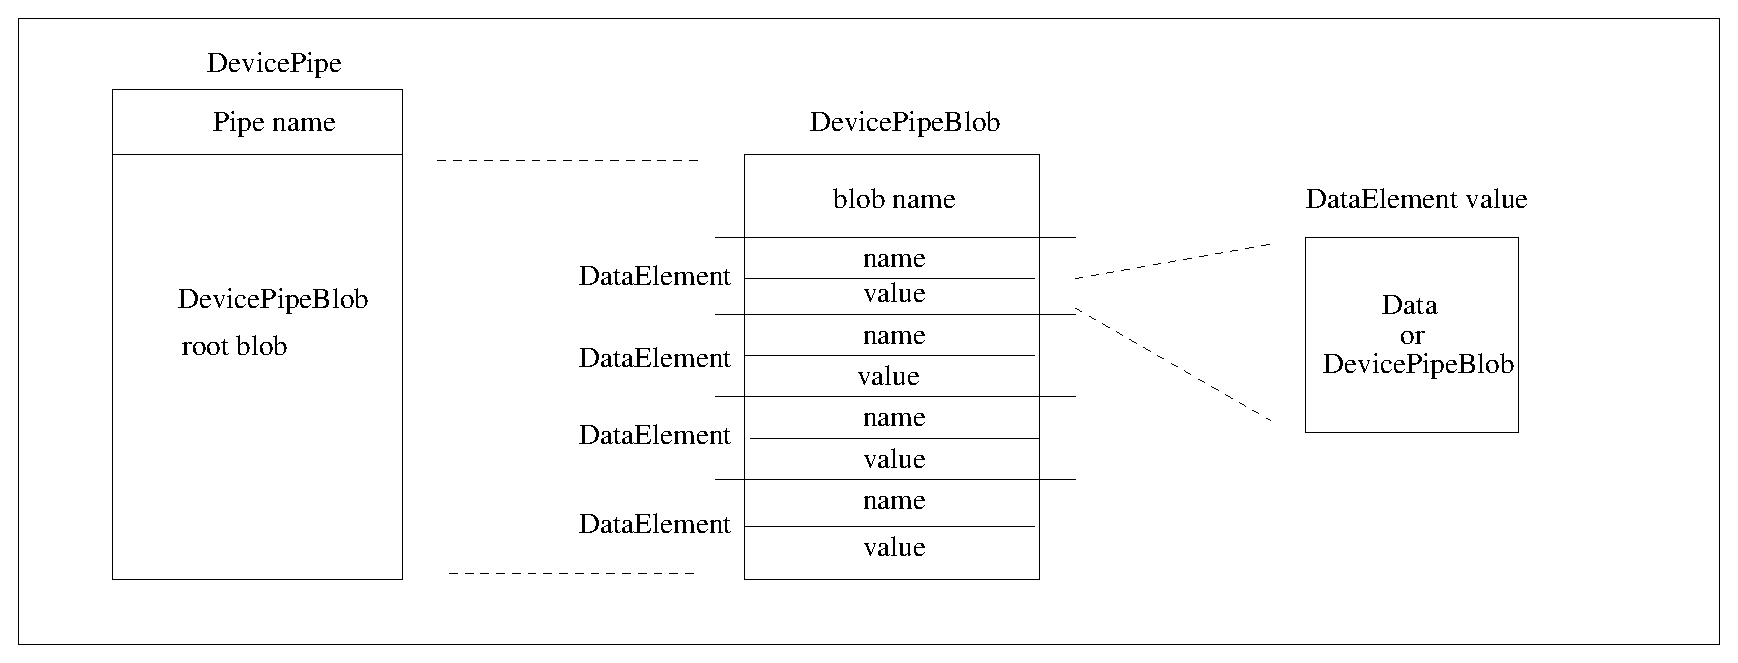
\includegraphics[width=14cm,height=8cm]{gen_api/pipe}
\par\end{centering}

\protect\caption{DevicePipe data structure\label{ }}
\end{figure}


Many methods to insert/extract data into/from a DevicePipe are available.
In the DevicePipe class, these methods simply forward their action
to the DevicePipe root blob. The same methods are available in the
DevicePipeBlob in case you need to use the recursivity provided by
this data structure.


\subsection{Reading a pipe}

When you read a pipe, you have to extract data received from the pipe.
Because data transferred through a pipe can change at any moment,
two differents cases are possible:
\begin{enumerate}
\item The client has a prior knowledge of what should be transferred through
the pipe
\item The client does not know at all what has been received through the
pipe
\end{enumerate}
Those two cases are detailed in the following sub-chapters.


\subsubsection{Extracting data with pipe content prior knowledge}

To extract data from a DevicePipe object (or from a DevicePipeBlob
object), you have to use its extraction operator \textquotedbl{}>\textcompwordmark{}>\textquotedbl{}.
Let's suppose that we already know (prior knowledge) that the pipe
contains 3 data elements with a Tango long, an array of double and
finally an array of unsigned short. The code you need to extract these
data is (Without error case treatment detailed in a next sub-chapter)

%
% Copyright (C) :      2004,2005,2006,2007,2008,2009,2010,2011,2012,2013
%                      European Synchrotron Radiation Facility
%                      BP 220, Grenoble 38043
%                      FRANCE
%
% This file is part of Tango.
%
% Tango is free software: you can redistribute it and/or modify
% it under the terms of the GNU Lesser General Public License as published by
% the Free Software Foundation, either version 3 of the License, or
% (at your option) any later version.
%
% Tango is distributed in the hope that it will be useful,
% but WITHOUT ANY WARRANTY; without even the implied warranty of
% MERCHANTABILITY or FITNESS FOR A PARTICULAR PURPOSE.  See the
% GNU Lesser General Public License for more details.
%
% You should have received a copy of the GNU Lesser General Public License
% along with Tango.  If not, see <http://www.gnu.org/licenses/>.
%
\begin{flushleft}
\begin{picture}(0,0)
\thicklines
\put(0,0){\line(1,0){400}}
\end{picture}
\end{flushleft}

\begin{lyxcode}
1~DevicePipe~dp~=~mydev.read\_pipe(\textquotedbl{}MyPipe\textquotedbl{});

2~

3~DevLong~dl;~~

4~vector<double>~v\_db;~~

5~DevVarUShortArray~{*}dvush~=~new~DevVarUShortArray();

6~

7~dp~>\textcompwordmark{}>~dl~>\textcompwordmark{}>~v\_db~>\textcompwordmark{}>~dvush;

8

9~delete~dvush;
\end{lyxcode}
%
% Copyright (C) :      2004,2005,2006,2007,2008,2009,2010,2011,2012,2013
%                      European Synchrotron Radiation Facility
%                      BP 220, Grenoble 38043
%                      FRANCE
%
% This file is part of Tango.
%
% Tango is free software: you can redistribute it and/or modify
% it under the terms of the GNU Lesser General Public License as published by
% the Free Software Foundation, either version 3 of the License, or
% (at your option) any later version.
%
% Tango is distributed in the hope that it will be useful,
% but WITHOUT ANY WARRANTY; without even the implied warranty of
% MERCHANTABILITY or FITNESS FOR A PARTICULAR PURPOSE.  See the
% GNU Lesser General Public License for more details.
%
% You should have received a copy of the GNU Lesser General Public License
% along with Tango.  If not, see <http://www.gnu.org/licenses/>.
%
\begin{flushleft}
\begin{picture}(0,0)
\thicklines
\put(0,0){\line(1,0){400}}
\end{picture}
\end{flushleft}


The pipe is read at line 1. Pipe (or root blob) data extracttion is
at line 7. As you can see, it is just a matter of chaining extraction
operator (\textquotedbl{}>\textcompwordmark{}>\textquotedbl{}) into
local data (declared line 3 to 5). In this example, the transported
array of double is extracted into a C++ vector while the unsigned
short array is extracted in a Tango sequence data type. When you extract
data into a vector, there is a unavoidable memory copy between the
DevicePipe object and the vector. When you extract data in a Tango
sequence data type, there is no memory copy but the extraction method
consumes the memory and it is therefore caller responsability to delete
the memory. This is the rule of line 9. If there is a DevicePipeBlob
inside the DevicePipe, simply extract it into one instance of the
DevicePipeBlob class.

You may notice that the pipe root blob data elements name are lost
in the previous example. The Tango API also has a DataElement\index{DataElement}
class which allows you to retrieve/set data element name. The following
code is how you can extract pipe data and retrieve data element name
(same pipe then previously)

%
% Copyright (C) :      2004,2005,2006,2007,2008,2009,2010,2011,2012,2013
%                      European Synchrotron Radiation Facility
%                      BP 220, Grenoble 38043
%                      FRANCE
%
% This file is part of Tango.
%
% Tango is free software: you can redistribute it and/or modify
% it under the terms of the GNU Lesser General Public License as published by
% the Free Software Foundation, either version 3 of the License, or
% (at your option) any later version.
%
% Tango is distributed in the hope that it will be useful,
% but WITHOUT ANY WARRANTY; without even the implied warranty of
% MERCHANTABILITY or FITNESS FOR A PARTICULAR PURPOSE.  See the
% GNU Lesser General Public License for more details.
%
% You should have received a copy of the GNU Lesser General Public License
% along with Tango.  If not, see <http://www.gnu.org/licenses/>.
%
\begin{flushleft}
\begin{picture}(0,0)
\thicklines
\put(0,0){\line(1,0){400}}
\end{picture}
\end{flushleft}

\begin{lyxcode}
1~DevicePipe~dp~=~mydev.read\_pipe(\textquotedbl{}MyPipe\textquotedbl{});

2~

3~DataElement<DevLong>~de\_dl;~~

4~DataElement<vector<double>~>~de\_v\_db;~~

5~DataElement<DevVarUShortArray~{*}>~de\_dvush(new~DevVarUShortArray());

6~

7~dp~>\textcompwordmark{}>~de\_dl~>\textcompwordmark{}>~de\_v\_db~>\textcompwordmark{}>~de\_dvush;

8

9~delete~de\_dvush.value;
\end{lyxcode}
%
% Copyright (C) :      2004,2005,2006,2007,2008,2009,2010,2011,2012,2013
%                      European Synchrotron Radiation Facility
%                      BP 220, Grenoble 38043
%                      FRANCE
%
% This file is part of Tango.
%
% Tango is free software: you can redistribute it and/or modify
% it under the terms of the GNU Lesser General Public License as published by
% the Free Software Foundation, either version 3 of the License, or
% (at your option) any later version.
%
% Tango is distributed in the hope that it will be useful,
% but WITHOUT ANY WARRANTY; without even the implied warranty of
% MERCHANTABILITY or FITNESS FOR A PARTICULAR PURPOSE.  See the
% GNU Lesser General Public License for more details.
%
% You should have received a copy of the GNU Lesser General Public License
% along with Tango.  If not, see <http://www.gnu.org/licenses/>.
%
\begin{flushleft}
\begin{picture}(0,0)
\thicklines
\put(0,0){\line(1,0){400}}
\end{picture}
\end{flushleft}


The extraction line (number 7) is similar to the previous case but
local data are instances of DataElement class. This is template class
and instances are created at lines 4 to 6. Each DataElement instance
has only two elements which are:
\begin{enumerate}
\item The data element name (a C++ string): \emph{name}
\item The data element value (One instance of the template parameter): \emph{value}
\end{enumerate}

\subsubsection{Extracting data in a generic way (without prior knowledge)}

Due to the dynamicity of the data transferred through a pipe, the
API alows to extract data from a pipe without any prior knowledge
of its content. This is achived with methods \emph{get\_data\_elt\_nb()},
\emph{get\_data\_elt\_type()}, \emph{get\_data\_elt\_name()} and the
extraction operator \textquotedbl{}>\textcompwordmark{}>\textquotedbl{}.
These methods belong to the DevicePipeBlob class but they also exist
on the DevicePipe class for its root blob. Here is one example of
how you use them:

%
% Copyright (C) :      2004,2005,2006,2007,2008,2009,2010,2011,2012,2013
%                      European Synchrotron Radiation Facility
%                      BP 220, Grenoble 38043
%                      FRANCE
%
% This file is part of Tango.
%
% Tango is free software: you can redistribute it and/or modify
% it under the terms of the GNU Lesser General Public License as published by
% the Free Software Foundation, either version 3 of the License, or
% (at your option) any later version.
%
% Tango is distributed in the hope that it will be useful,
% but WITHOUT ANY WARRANTY; without even the implied warranty of
% MERCHANTABILITY or FITNESS FOR A PARTICULAR PURPOSE.  See the
% GNU Lesser General Public License for more details.
%
% You should have received a copy of the GNU Lesser General Public License
% along with Tango.  If not, see <http://www.gnu.org/licenses/>.
%
\begin{flushleft}
\begin{picture}(0,0)
\thicklines
\put(0,0){\line(1,0){400}}
\end{picture}
\end{flushleft}

\begin{lyxcode}
1~~DevicePipe~dp~=~mydev.read\_pipe(\textquotedbl{}MyPipe\textquotedbl{});

2

3~~size\_t~nb\_de~=~dp.get\_data\_elt\_nb();~~

4~~for~(size\_t~loop~=~0;loop~<~nb;loop++)

5~~\{~~~~~~

6~~~~~int~data\_type~=~dp.get\_data\_elt\_type(loop);~~~~~~

7~~~~~string~de\_name~=~dp.get\_data\_elt\_name(loop);~~~~~~

8~~~~~switch(data\_type)~~~~~~

9~~~~~\{~~~~~~~~~

10~~~~~~~~case~DEV\_LONG:~~~~~~~~~

11~~~~~~~~\{~~~~~~~~~~~~~

12~~~~~~~~~~~~DevLong~lg;~~~~~~~~~~~~~

13~~~~~~~~~~~~dp~>\textcompwordmark{}>~lg;~~~~~~~~~

14~~~~~~~~\}~~~~~~~~~

15~~~~~~~~break;

16~~~~~~~~

17~~~~~~~~case~DEVVAR\_DOUBLEARRAY:~~~~~~~~~

18~~~~~~~~\{~~~~~~~~~~~~~

19~~~~~~~~~~~~vector<double>~v\_db;~~~~~~~~~~~~~

20~~~~~~~~~~~~dp~>\textcompwordmark{}>~v\_db;~~~~~~~~~

21~~~~~~~~\}~~~~~~~~~

22~~~~~~~~break;~~~~~~~~~

23~~~~~~~~....~~~~~~

24~~~~\}~~

25~~~~...~~

26~\}
\end{lyxcode}
%
% Copyright (C) :      2004,2005,2006,2007,2008,2009,2010,2011,2012,2013
%                      European Synchrotron Radiation Facility
%                      BP 220, Grenoble 38043
%                      FRANCE
%
% This file is part of Tango.
%
% Tango is free software: you can redistribute it and/or modify
% it under the terms of the GNU Lesser General Public License as published by
% the Free Software Foundation, either version 3 of the License, or
% (at your option) any later version.
%
% Tango is distributed in the hope that it will be useful,
% but WITHOUT ANY WARRANTY; without even the implied warranty of
% MERCHANTABILITY or FITNESS FOR A PARTICULAR PURPOSE.  See the
% GNU Lesser General Public License for more details.
%
% You should have received a copy of the GNU Lesser General Public License
% along with Tango.  If not, see <http://www.gnu.org/licenses/>.
%
\begin{flushleft}
\begin{picture}(0,0)
\thicklines
\put(0,0){\line(1,0){400}}
\end{picture}
\end{flushleft}


The number of data element in the pipe root blob is retrieve at line
3. Then a loop for each data element is coded. For each data element,
its value data type and its name are retrieved at lines 6 and 7. Then,
according to the data element value data type, the data are extracted
using the classical extraction operator (lines 13 or 20)


\subsubsection{Error management}

By default, in case of error, the DevicePipe object throws different
kind of exceptions according to the error kind. It is possible to
disable exception throwing. If you do so, the code has to test the
DevicePipe state after extraction. The possible error cases are:
\begin{itemize}
\item DevicePipe object is empty
\item Wrong data type for extraction (For instance extraction into a double
data while the DataElement contains a string)
\item Wrong number of DataElement (Extraction code extract 5 data element
while the pipe contains only four)
\item Mix of extraction (or insertion) method kind (classical operators
<\textcompwordmark{}< or >\textcompwordmark{}>) and {[}{]} operator.
\end{itemize}
Methods \emph{exceptions()} and \emph{reset\_exceptions()} of the
DevicePipe and DevicePipeBlob classes allow the user to select which
kind of error he is interested in. For error treatment without exceptions,
methods \emph{has\_failed()} and \emph{state()} has to be used. See
reference documentation for details about these methods.


\subsection{Writing a pipe}

Writing data into a DevicePipe or a DevicePipeBlob is similar to reading
data from a pipe. The main method is the insertion operator \textquotedbl{}<\textcompwordmark{}<\textquotedbl{}.
Let's have a look at a first example if you want to write a pipe with
a Tango long, a vector of double and finally an array of unsigned
short.

%
% Copyright (C) :      2004,2005,2006,2007,2008,2009,2010,2011,2012,2013
%                      European Synchrotron Radiation Facility
%                      BP 220, Grenoble 38043
%                      FRANCE
%
% This file is part of Tango.
%
% Tango is free software: you can redistribute it and/or modify
% it under the terms of the GNU Lesser General Public License as published by
% the Free Software Foundation, either version 3 of the License, or
% (at your option) any later version.
%
% Tango is distributed in the hope that it will be useful,
% but WITHOUT ANY WARRANTY; without even the implied warranty of
% MERCHANTABILITY or FITNESS FOR A PARTICULAR PURPOSE.  See the
% GNU Lesser General Public License for more details.
%
% You should have received a copy of the GNU Lesser General Public License
% along with Tango.  If not, see <http://www.gnu.org/licenses/>.
%
\begin{flushleft}
\begin{picture}(0,0)
\thicklines
\put(0,0){\line(1,0){400}}
\end{picture}
\end{flushleft}

\begin{lyxcode}
1~~DevicePipe~dp(\textquotedbl{}MyPipe\textquotedbl{});

2~

3~~vector<string>~de\_names~\{\textquotedbl{}FirstDE\textquotedbl{},\textquotedbl{}SecondDE\textquotedbl{},\textquotedbl{}ThirdDE\textquotedbl{}\};

4~~db.set\_data\_elt\_names(de\_names);

5

6~~DevLong~dl~=~666;~~

7~~vector<double>~v\_db~\{1.11,2.22\};

8~~unsigned~short~{*}array~=~new~unsigned~short~{[}100{]};

9~~DevVarUShortArray~{*}dvush~=~create\_DevVarUShortArray(array,100);

10

11~try~~

12~\{~~~~~

12~~~~dp~<\textcompwordmark{}<~dl~<\textcompwordmark{}<~v\_db~<\textcompwordmark{}<~dvush;

13~~~~mydev.write\_pipe(dp);

14~\}

15~catch~(DevFailed~\&e)

16~\{~~~~~

17~~~~cout~<\textcompwordmark{}<~\textquotedbl{}DevicePipeBlob~insertion~failed\textquotedbl{}~<\textcompwordmark{}<~endl;~~~~~

18~~~~....~~

19~\}
\end{lyxcode}
%
% Copyright (C) :      2004,2005,2006,2007,2008,2009,2010,2011,2012,2013
%                      European Synchrotron Radiation Facility
%                      BP 220, Grenoble 38043
%                      FRANCE
%
% This file is part of Tango.
%
% Tango is free software: you can redistribute it and/or modify
% it under the terms of the GNU Lesser General Public License as published by
% the Free Software Foundation, either version 3 of the License, or
% (at your option) any later version.
%
% Tango is distributed in the hope that it will be useful,
% but WITHOUT ANY WARRANTY; without even the implied warranty of
% MERCHANTABILITY or FITNESS FOR A PARTICULAR PURPOSE.  See the
% GNU Lesser General Public License for more details.
%
% You should have received a copy of the GNU Lesser General Public License
% along with Tango.  If not, see <http://www.gnu.org/licenses/>.
%
\begin{flushleft}
\begin{picture}(0,0)
\thicklines
\put(0,0){\line(1,0){400}}
\end{picture}
\end{flushleft}


Insertion into the DevicePipe is done at line 12 with the insert operators.
The main difference with extracting data from the pipe is at line
3 and 4. When inserting data into a pipe, you need to FIRST define
its number od name of data elements. In our example, the device pipe
is initialized to carry three data element and the names of these
data elements is defined at line 4. This is a mandatory requirement.
If you don't define data element number, exception will be thrown
during the use of insertion methods. The population of the array used
for the third pipe data element is not represented here.

It's also possible to use DataElement class instances to set the pipe
data element. Here is the previous example modified to use DataElement
class.

%
% Copyright (C) :      2004,2005,2006,2007,2008,2009,2010,2011,2012,2013
%                      European Synchrotron Radiation Facility
%                      BP 220, Grenoble 38043
%                      FRANCE
%
% This file is part of Tango.
%
% Tango is free software: you can redistribute it and/or modify
% it under the terms of the GNU Lesser General Public License as published by
% the Free Software Foundation, either version 3 of the License, or
% (at your option) any later version.
%
% Tango is distributed in the hope that it will be useful,
% but WITHOUT ANY WARRANTY; without even the implied warranty of
% MERCHANTABILITY or FITNESS FOR A PARTICULAR PURPOSE.  See the
% GNU Lesser General Public License for more details.
%
% You should have received a copy of the GNU Lesser General Public License
% along with Tango.  If not, see <http://www.gnu.org/licenses/>.
%
\begin{flushleft}
\begin{picture}(0,0)
\thicklines
\put(0,0){\line(1,0){400}}
\end{picture}
\end{flushleft}

\begin{lyxcode}
1~~DevicePipe~dp(\textquotedbl{}MyPipe\textquotedbl{});

2

3~~DataElement<DevLong>~de\_dl(\textquotedbl{}FirstElt\textquotedbl{},666);~~

4~~vector<double>~~v\_db~\{1.11,2.22\};

5~~DataElement<vector<double>~>~de\_v\_db(\textquotedbl{}SecondElt,v\_db);

6

7~~unsigned~short~{*}array~=~new~unsigned~short~{[}100{]};

8~~DevVarUShortArray~{*}dvush~=~create\_DevVarUShortArray(array,100);

9~~DataElement<DevVarUShortArray~{*}>~de\_dvush(\textquotedbl{}ThirdDE\textquotedbl{},array);

10

11~try~~

12~\{~~~~~

12~~~~dp~<\textcompwordmark{}<~de\_dl~<\textcompwordmark{}<~de\_v\_db~<\textcompwordmark{}<~de\_dvush;

13~~~~mydev.write\_pipe(dp);

14~\}

15~catch~(DevFailed~\&e)

16~\{~~~~~

17~~~~cout~<\textcompwordmark{}<~\textquotedbl{}DevicePipeBlob~insertion~failed\textquotedbl{}~<\textcompwordmark{}<~endl;~~~~~

18~~~~....~~

19~\}
\end{lyxcode}
%
% Copyright (C) :      2004,2005,2006,2007,2008,2009,2010,2011,2012,2013
%                      European Synchrotron Radiation Facility
%                      BP 220, Grenoble 38043
%                      FRANCE
%
% This file is part of Tango.
%
% Tango is free software: you can redistribute it and/or modify
% it under the terms of the GNU Lesser General Public License as published by
% the Free Software Foundation, either version 3 of the License, or
% (at your option) any later version.
%
% Tango is distributed in the hope that it will be useful,
% but WITHOUT ANY WARRANTY; without even the implied warranty of
% MERCHANTABILITY or FITNESS FOR A PARTICULAR PURPOSE.  See the
% GNU Lesser General Public License for more details.
%
% You should have received a copy of the GNU Lesser General Public License
% along with Tango.  If not, see <http://www.gnu.org/licenses/>.
%
\begin{flushleft}
\begin{picture}(0,0)
\thicklines
\put(0,0){\line(1,0){400}}
\end{picture}
\end{flushleft}


The population of the array used for the third pipe data element is
not represented here. Finally, there is a third way to insert data
into a device pipe. You have to defined number and names of the data
element within the pipe (similar to first insertion method) but you
are able to insert data into the data element in any order using the
\textquotedbl{}{[}{]}\textquotedbl{} operator overwritten for the
DevicePipe and DevicePipeBlob classes. Look at the following example:

%
% Copyright (C) :      2004,2005,2006,2007,2008,2009,2010,2011,2012,2013
%                      European Synchrotron Radiation Facility
%                      BP 220, Grenoble 38043
%                      FRANCE
%
% This file is part of Tango.
%
% Tango is free software: you can redistribute it and/or modify
% it under the terms of the GNU Lesser General Public License as published by
% the Free Software Foundation, either version 3 of the License, or
% (at your option) any later version.
%
% Tango is distributed in the hope that it will be useful,
% but WITHOUT ANY WARRANTY; without even the implied warranty of
% MERCHANTABILITY or FITNESS FOR A PARTICULAR PURPOSE.  See the
% GNU Lesser General Public License for more details.
%
% You should have received a copy of the GNU Lesser General Public License
% along with Tango.  If not, see <http://www.gnu.org/licenses/>.
%
\begin{flushleft}
\begin{picture}(0,0)
\thicklines
\put(0,0){\line(1,0){400}}
\end{picture}
\end{flushleft}

\begin{lyxcode}
1~~DevicePipe~dp(\textquotedbl{}MyPipe\textquotedbl{});

2~

3~~vector<string>~de\_names~\{\textquotedbl{}FirstDE\textquotedbl{},\textquotedbl{}SecondDE\textquotedbl{},\textquotedbl{}ThirdDE\textquotedbl{}\};

4~~db.set\_data\_elt\_names(de\_names);

5

6~~DevLong~dl~=~666;~~

7~~vector<double>~v\_db~=~\{1.11,2.22\};

8~~unsigned~short~{*}array~=~new~unsigned~short~{[}100{]};

9~~DevVarUShortArray~{*}dvush~=~create\_DevVarUShortArray(array,100);

10

11~dp{[}\textquotedbl{}SecondDE\textquotedbl{}{]}~<\textcompwordmark{}<~v\_db;

12~dp{[}\textquotedbl{}FirstDE\textquotedbl{}{]}~<\textcompwordmark{}<~dl;

13~dp{[}\textquotedbl{}ThirdDE\textquotedbl{}{]}~<\textcompwordmark{}<~dvush;
\end{lyxcode}
%
% Copyright (C) :      2004,2005,2006,2007,2008,2009,2010,2011,2012,2013
%                      European Synchrotron Radiation Facility
%                      BP 220, Grenoble 38043
%                      FRANCE
%
% This file is part of Tango.
%
% Tango is free software: you can redistribute it and/or modify
% it under the terms of the GNU Lesser General Public License as published by
% the Free Software Foundation, either version 3 of the License, or
% (at your option) any later version.
%
% Tango is distributed in the hope that it will be useful,
% but WITHOUT ANY WARRANTY; without even the implied warranty of
% MERCHANTABILITY or FITNESS FOR A PARTICULAR PURPOSE.  See the
% GNU Lesser General Public License for more details.
%
% You should have received a copy of the GNU Lesser General Public License
% along with Tango.  If not, see <http://www.gnu.org/licenses/>.
%
\begin{flushleft}
\begin{picture}(0,0)
\thicklines
\put(0,0){\line(1,0){400}}
\end{picture}
\end{flushleft}


Insertion into the device pipe is now done at lines 11 to 13. The
population of the array used for the third pipe data element is not
represented here. Note that the data element name is case insensitive.


\subsubsection{Error management}

When inserting data into a DevicePipe or a DevicePipeBlob, error management
is very similar to reading data from from a DevicePipe or a DevicePipeBlob.
The difference is that there is one moer case which could trigger
one exception during the insertion. This case is
\begin{itemize}
\item Insertion into the DevicePipe (or DevicePipeBlob) if its data element
number have not been set.
\end{itemize}

\section{Device locking\index{Locking}}

Starting with Tango release 7 (and device inheriting from Device\_4Impl),
device locking is supported. For instance, this feature could be used
by an application doing a scan on a synchrotron beam line. In such
a case, you want to move an actuator then read a sensor, move the
actuator again, read the sensor...You don't want the actuator to be
moved by another client while the application is doing the scan. If
the application doing the scan locks the actuator device, it will
be sure that this device is \textquotedbl{}reserved\textquotedbl{}
for the application doing the scan and other client will not be able
to move it until the scan application un-locks this actuator.

A locked device is protected against:
\begin{itemize}
\item \emph{command\_inout} call except for device state and status requested
via command and for the set of commands defined as allowed following
the definition of allowed command in the Tango control access schema.
\item \emph{write\_attribute} and \emph{write\_pipe} call
\item \emph{write\_read\_attribute, write\_read\_attributes} and \emph{write\_read\_pipe}
call
\item \emph{set\_attribute\_config }and\emph{ set\_pipe\_config} call
\item polling and logging commands related to the locked device
\end{itemize}
Other clients trying to do one of these calls on a locked device will
get a DevFailed exception. In case of application with locked device
crashed, the lock will be automatically release after a defined interval.
The API provides a set of methods for application code to lock/unlock
device. These methods are:
\begin{itemize}
\item \emph{DeviceProxy::lock()} and \emph{DeviceProxy::unlock()} to lock/unlock
device
\item \emph{DeviceProxy::locking\_status()}, \emph{DeviceProxy::is\_locked()},
\emph{DeviceProxy::is\_locked\_by\_me()} and \emph{DeviceProxy::get\_locker()}
to get locking information
\end{itemize}
These methods are precisely described in the API reference chapters.


\section{Reconnection\index{reconnection} and exception}

The Tango API automatically manages re-connection between client and
server in case of communication error during a network access between
a client and a server. By default, when a communication error occurs,
an exception is returned to the caller and the connection is internally
marked as bad. On the next try to contact the device, the API will
try to re-build the network connection. With the \emph{set\_transparency\_reconnection\index{set-transparency-reconnection}()}
method of the DeviceProxy\index{DeviceProxy} class, it is even possible
not to have any exception thrown in case of communication error. The
API will try to re-build the network connection as soon as it is detected
as bad. This is the default mode. See \ref{sec:Reconnection-and-exception}
for more details on this subject.


\section{Thread\index{thread} safety}

Starting with Tango 7.2, some classes of the C++ API has been made
thread safe. These classes are:
\begin{itemize}
\item DeviceProxy
\item Database
\item Group
\item ApiUtil
\item AttributeProxy
\end{itemize}
This means that it is possible to share between threads a pointer
to a DeviceProxy instance. It is safe to execute a call on this DeviceProxy
instance while another thread is also doing a call to the same DeviceProxy
instance. Obviously, this also means that it is possible to create
thread local DeviceProxy instances and to execute method calls on
these instances. Nevertheless, data local to a DeviceProxy instance
like its timeout are not managed on a per thread basis. For a DeviceProxy
instance shared between two threads, if thread 1 changes the instance
timeout, thread 2 will also see this change.


\section{Compiling and linking a Tango client}

Compiling and linking a Tango client is similar to compiling and linking
a Tango device server. Please, refer to chapter \textquotedbl{}Compiling,
Linking and executing a Tango device server process\textquotedbl{}
(\ref{sec:Compiling,-linking-and}) to get all the details.

\begin{center}

\label{ThreeRicardo}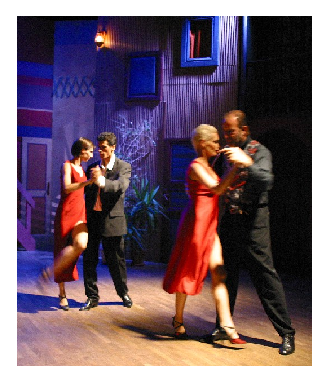
\includegraphics[scale=2]{dance/0066-reduc}

\end{center}


\begin{comment}
The Tango ATK 
\end{comment}


\chapter{TangoATK Programmer's Guide}

This chapter is only a brief Tango ATK (Application ToolKit) programmer's
guide. You can find a reference guide with a full description of TangoATK
classes and methods in the ATK JavaDoc \cite{ATK-doc}.

A tutorial document \cite{ATK-Tutorial} is also provided and includes
the detailed description of the ATK architecture and the ATK components.
In the ATK Tutorial \cite{ATK-Tutorial} you can find some code examples
and also Flash Demos which explain how to start using Tango ATK.


\section{Introduction}

This document describes how to develop applications using the Tango
Application Toolkit, TangoATK for short. It will start with a brief
description of the main concepts behind the toolkit, and then continue
with more practical, real-life examples to explain key parts.


\subsection{Assumptions}

The author assumes that the reader has a good knowledge of the Java
programming language, and a thorough understanding of object-oriented
programming. Also, it is expected that the reader is fluent in all
aspects regarding Tango devices, attributes, and commands.


\section{The key concepts of TangoATK}

TangoATK was developed with these goals in mind
\begin{itemize}
\item TangoATK should help minimize development time 
\item TangoATK should help minimize bugs in applications 
\item TangoATK should support applications that contain attributes and commands
from several different devices. 
\item TangoATK should help avoid code duplication. 
\end{itemize}
Since most Tango-applications were foreseen to be displayed on some
sort of graphic terminal, TangoATK needed to provide support for some
sort of graphic building blocks. To enable this, and since the toolkit
was to be written in Java, we looked to Swing to figure out how to
do this.

Swing is developed using a variant over a design-pattern the Model-View-Controller\index{Model-View-Controller}
(MVC\index{MVC}) pattern called \emph{model-delegate}, where the
view and the controller of the MVC-pattern are merged into one object.

\begin{center}
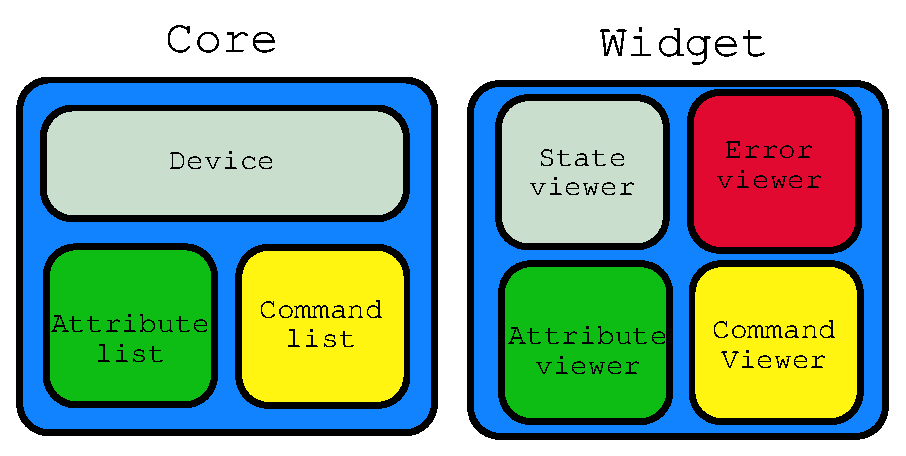
\includegraphics[scale=0.6]{atk/img/core-widget}\\

\par\end{center}

This pattern made the choice of labor division quite easy: all non-graphic
parts of TangoATK reside in the packages beneath \texttt{fr.esrf.tangoatk.core}\index{model}\index{core},
and anything remotely graphic are located beneath \texttt{fr.esrf.tangoatk.widge}t\index{viewer}\index{widget}.
More on the content and organization of this will follow.

The communication between the non-graphic and graphic objects are
done by having the graphic object registering itself as a listener
to the non-graphic object, and the non-graphic object emmiting events
telling the listeners that its state has changed.


\subsection{Minimize development time}

For TangoATK to help minimize the development time of graphic applications,
the toolkit has been developed along two lines of thought
\begin{itemize}
\item Things that are needed in most applications are included, eg \texttt{Splash},
a splash\index{splash} window which gives a graphical way for the
application to show the progress of a long operation. The splash window
is moslty used in the startup phase of the application.
\item Building blocks provided by TangoATK should be easy to use and follow
certain patterns, eg every graphic widget has a \texttt{setModel}
method which is used to connect the widget with its non-graphic model. 
\end{itemize}
In addition to this, TangoATK provides a framework for error handling,
something that is often a time consuming task.


\subsection{Minimize bugs in applications}

Together with the Tango API, TangoATK takes care of most of the hard
things related to programming with Tango. Using TangoATK the developer
can focus on developing her application, not on understanding Tango.


\subsection{Attributes and commands from different devices}

To be able to create applications with attributes\index{attributes}
and commands\index{commands} from different devices, it was decided
that the central objects of TangoATK were not to be the device\index{device},
but rather the \emph{attributes and the commands}. This will certainly
feel a bit awkward at first, but trust me, the design holds.

For this design to be feasible, a structure was needed to keep track
of the commands and attributes, so the \emph{command-list\index{command-list}
and the attribute-list\index{attribte-list}} was introduced. These
two objects can hold commands and attributes from any number of devices.


\subsection{Avoid code duplication}

When writing applications for a control-system without a framework
much code is duplicated. Anything from simple widgets for showing
numeric values to error handling has to be implemented each time.
TangoATK supplies a number of frequently used widgets along with a
framework for connecting these widgets with their non-graphic counterparts.
Because of this, the developer only needs to write the \emph{glue}
- the code which connects these objects in a manner that suits the
specified application.


\section{The real getting started}

Generally there are two kinds of end-user applications: Applications
that only know how to treat one device, and applications that treat
many devices.


\subsection{Single device applications}

Single device applications are quite easy to write, even with a gui.
The following steps are required
\begin{enumerate}
\item Instantiate an AttributeList\index{AttributeList} and fill it with
the attributes you want. 
\item Instantiate a CommandList\index{CommandList} and fill it with the
commands you want. 
\item Connect the whole \emph{AttributeList} with a \emph{list viewer} and
/ or each \emph{individual attribute} with an \emph{attribute viewer}. 
\item Connect the whole \emph{CommandList} to a \emph{command list viewer}
and / or connect each \emph{individual command} in the command list
with a \emph{command viewer}. 
\end{enumerate}
\begin{center}
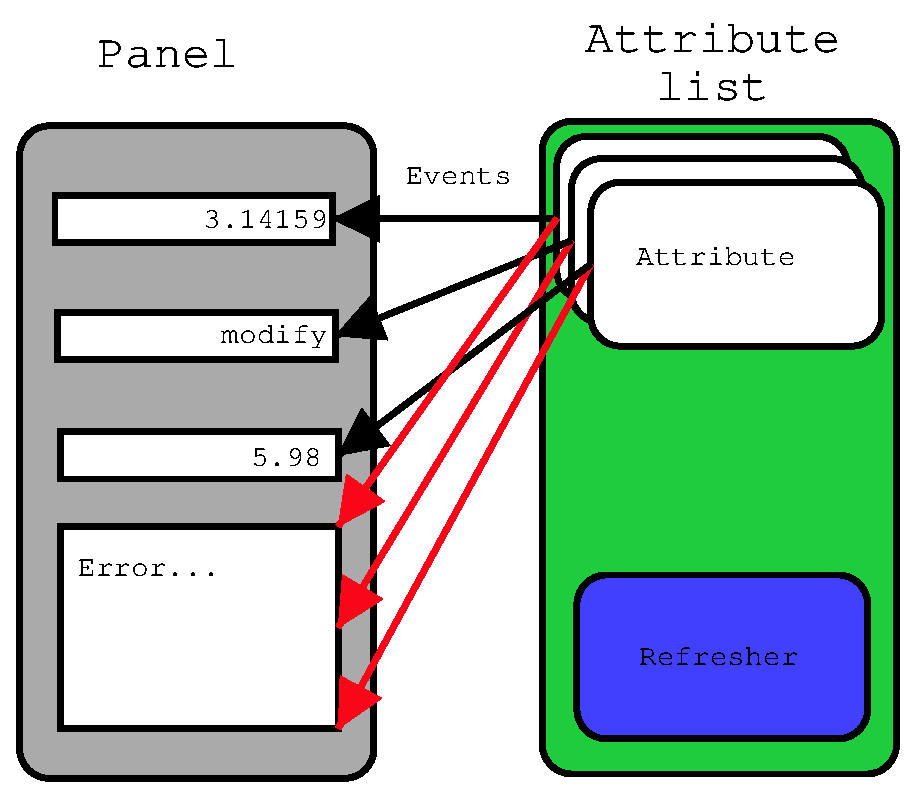
\includegraphics[scale=0.6]{atk/img/listpanel}
\par\end{center}

The following program (FirstApplication)\index{ScalarListViewer}
shows an implementation of the list mentioned above. It should be
rather self-explanatory with the comments.


\begin{minted}[linenos]{cpp}
package examples;
 

import javax.swing.JFrame;
import javax.swing.JMenuItem;
import javax.swing.JMenuBar;
import javax.swing.JMenu;
 

import java.awt.event.ActionListener;
import java.awt.event.ActionEvent;
import java.awt.BorderLayout;
 

import fr.esrf.tangoatk.core.AttributeList;
import fr.esrf.tangoatk.core.ConnectionException;
 

import fr.esrf.tangoatk.core.CommandList;
import fr.esrf.tangoatk.widget.util.ErrorHistory;
import fr.esrf.tangoatk.widget.util.ATKGraphicsUtils;
import fr.esrf.tangoatk.widget.attribute.ScalarListViewer;
import fr.esrf.tangoatk.widget.command.CommandComboViewer;
 

public class FirstApplication extends JFrame
{
JMenuBar menu;                    // So that our application looks
                                  // halfway decent.
AttributeList attributes;         // The list that will contain our
                                  // attributes
CommandList commands;             // The list that will contain our
                                  // commands
ErrorHistory errorHistory;        // A window that displays errors
ScalarListViewer sListViewer;     // A viewer which knows how to
                                  // display a list of scalar attributes.
                                  // If you want to display other types
                                  // than scalars, you'll have to wait
                                  // for the next example.
CommandComboViewer commandViewer; // A viewer which knows how to display
                                  // a combobox of commands and execute
                                  // them.
String device;                    // The name of our device.
 

public FirstApplication()
{
   // The swing stuff to create the menu bar and its pulldown menus
   menu = new JMenuBar();
   JMenu fileMenu = new JMenu();
   fileMenu.setText("File");   
   JMenu viewMenu = new JMenu();
   viewMenu.setText("View");

   JMenuItem quitItem = new JMenuItem();
   quitItem.setText("Quit");
   quitItem.addActionListener(new 
      java.awt.event.ActionListener()
      {                 
       public void
       actionPerformed(ActionEvent evt)
       {quitItemActionPerformed(evt);}
      });
   fileMenu.add(quitItem);

   JMenuItem errorHistItem = new JMenuItem();
   errorHistItem.setText("Error History");
   errorHistItem.addActionListener(new 
           java.awt.event.ActionListener()
           {                 
            public void 
            actionPerformed(ActionEvent evt)
            {errHistItemActionPerformed(evt);}
           });
   viewMenu.add(errorHistItem);
   menu.add(fileMenu);
   menu.add(viewMenu);

   //
   // Here we create ATK objects to handle attributes, commands and errors.
   //
   attributes = new AttributeList(); 
   commands = new CommandList();
   errorHistory = new ErrorHistory();
   device = "id14/eh3_mirror/1";
   sListViewer = new ScalarListViewer();
   commandViewer = new CommandComboViewer();


// 
// A feature of the command and attribute list is that if you
// supply an errorlistener to these lists, they'll add that
// errorlistener to all subsequently created attributes or
// commands. So it is important to do this _before_ you
// start adding attributes or commands.
//
 
   attributes.addErrorListener(errorHistory);
   commands.addErrorListener(errorHistory);
 
//
// Sometimes we're out of luck and the device or the attributes
// are not available. In that case a ConnectionException is thrown.
// This is why we add the attributes in a try/catch
//
 
   try
   {
 
//
// Another feature of the attribute and command list is that they
// can add wildcard names, currently only `*' is supported.
// When using a wildcard, the lists will add all commands or
// attributes available on the device.
//
   attributes.add(device + "/*");
   }
   catch (ConnectionException ce)
   {
      System.out.println("Error fetching " + 
                         "attributes from " +
                         device + " " + ce);
   }
 

//
// See the comments for attributelist
//
 

   try
   {
      commands.add(device + "/*");
   }
   catch (ConnectionException ce)
   {
      System.out.println("Error fetching " +
                         "commands from " +
                         device + " " + ce);
   }
 

//
// Here we tell the scalarViewer what it's to show. The
// ScalarListViewer loops through the attribute-list and picks out
// the ones which are scalars and show them.
//

   sListViewer.setModel(attributes);
 

//
// This is where the CommandComboViewer is told what it's to
// show. It knows how to show and execute most commands.
//
 

   commandViewer.setModel(commands);
 

//
// add the menubar to the frame
//
 

   setJMenuBar(menu);
 

//
// Make the layout nice.
//
 

   getContentPane().setLayout(new BorderLayout());
   getContentPane().add(commandViewer, BorderLayout.NORTH);
   getContentPane().add(sListViewer, BorderLayout.SOUTH);
 

//
// A third feature of the attributelist is that it knows how
// to refresh its attributes.
//
 

   attributes.startRefresher();
 

//
// JFrame stuff to make the thing show.
//
 

   pack();
   ATKGraphicsUtils.centerFrameOnScreen(this); //ATK utility to center window

   setVisible(true);
   }
 

   public static void main(String [] args)
   {
      new FirstApplication();
   }

   public void quitItemActionPerformed(ActionEvent evt)
   {
      System.exit(0);
   }

   public void errHistItemActionPerformed(ActionEvent evt)
   {
      errorHistory.setVisible(true);
   }
}



\end{minted}


The program should look something like this (depending on your platform
and your device)

\begin{center}
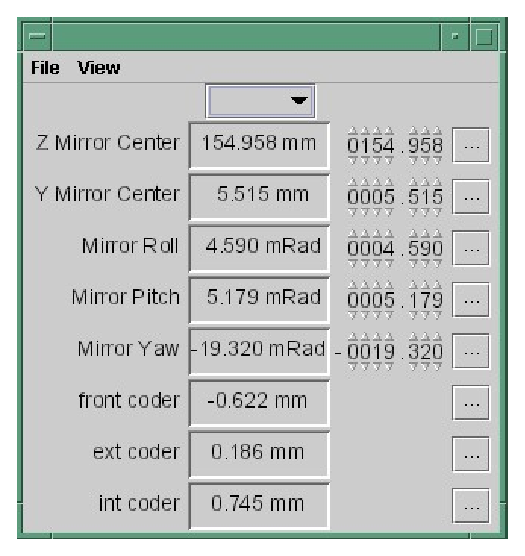
\includegraphics[scale=0.75]{atk/img/prog_guide_exple1}
\par\end{center}


\subsection{Multi device applications}

Multi device applications are quite similar to the single device applications,
the only difference is that it does not suffice to add the attributes
by wildcard, you need to add them explicitly, like this: \\



\begin{minted}[linenos]{cpp}
try
{ 
    // a StringScalar attribute from the device one
   attributes.add("jlp/test/1/att_cinq");
   // a NumberSpectrum attribute from the device one
   attributes.add("jlp/test/1/att_spectrum");
   // a NumberImage attribute from the device two
   attributes.add("sr/d-ipc/id25-1n/Image");
}
catch (ConnectionException ce)
{
   System.out.println("Error fetching " + 
       "attributes" + ce);
}

\end{minted}


The same goes for commands.


\subsection{More on displaying attributes}

So far, we've only considered scalar\index{scalar} attributes, and
not only that, we've also cheated quite a bit since we just passed
the attribute list to the \texttt{fr.esrf.tangoatk.widget.attribute.ScalarListViewer}
and let it do all the magic. The attribute list viewers are only available
for scalar attributes (NumberScalarListViewer\index{NumberScalarListViewer}
and ScalarListViewer\index{ScalarListViewer}). If you have one or
several spectrum\index{spectrum} or image\index{image} attributes
you must connect each spectrum or image attribute to it's corresponding
attribute viewer individually. So let's take a look at how you can
connect individual attributes (and not a whole attribute list) to
an individual attribute viewer (and not to an attribute list viewer).


\subsubsection{Connecting an attribute\index{model} to a viewer\index{viewer}}

Generally it is done in the following way:
\begin{enumerate}
\item You retrieve the attribute from the attribute list 
\item You instantiate the viewer 
\item Your call the \texttt{setModel\index{setModel}} method on the viewer
with the attribute as argument. 
\item You add your viewer to some panel
\end{enumerate}
The following example (SecondApplication)\index{SimpleScalarViewer}\index{NumberImageViewer}\index{NumberSpectrumViewer},
is a Multi-device application. Since this application uses individual
attribute viewers and not an attribute list viewer, it shows an implementation
of the list mentioned above.


\begin{minted}[linenos]{cpp}
package examples;
 

import javax.swing.JFrame;
import javax.swing.JMenuItem;
import javax.swing.JMenuBar;
import javax.swing.JMenu;
 

import java.awt.event.ActionListener;
import java.awt.event.ActionEvent;
import java.awt.BorderLayout;
import java.awt.Color;
 

import fr.esrf.tangoatk.core.AttributeList;
import fr.esrf.tangoatk.core.ConnectionException;
 
import fr.esrf.tangoatk.core.IStringScalar;
import fr.esrf.tangoatk.core.INumberSpectrum;
import fr.esrf.tangoatk.core.INumberImage;
import fr.esrf.tangoatk.widget.util.ErrorHistory;
import fr.esrf.tangoatk.widget.util.Gradient;
import fr.esrf.tangoatk.widget.util.ATKGraphicsUtils;
import fr.esrf.tangoatk.widget.attribute.NumberImageViewer;
import fr.esrf.tangoatk.widget.attribute.NumberSpectrumViewer;
import fr.esrf.tangoatk.widget.attribute.SimpleScalarViewer;

public class SecondApplication extends JFrame
{
     JMenuBar            menu;
     AttributeList       attributes;   // The list that will contain our attributes
     ErrorHistory        errorHistory; // A window that displays errors
     IStringScalar        ssAtt;
     INumberSpectrum      nsAtt;
     INumberImage         niAtt;
     public SecondApplication()
     {
        // Swing stuff to create the menu bar and its pulldown menus
        menu = new JMenuBar();
        JMenu fileMenu = new JMenu();
        fileMenu.setText("File");   
        JMenu viewMenu = new JMenu();
        viewMenu.setText("View");
        JMenuItem quitItem = new JMenuItem();
        quitItem.setText("Quit");
        quitItem.addActionListener(new java.awt.event.ActionListener()
                                      {                 
                                       public void actionPerformed(ActionEvent evt)
                                       {quitItemActionPerformed(evt);}
                                      });

        fileMenu.add(quitItem);
        JMenuItem errorHistItem = new JMenuItem();
        errorHistItem.setText("Error History");
        errorHistItem.addActionListener(new java.awt.event.ActionListener()
                {                 
                 public void actionPerformed(ActionEvent evt)
                 {errHistItemActionPerformed(evt);}
                });
        viewMenu.add(errorHistItem);
        menu.add(fileMenu);
        menu.add(viewMenu);
      //
      // Here we create TangoATK objects to view attributes and errors.
      //
        attributes = new AttributeList(); 
        errorHistory = new ErrorHistory();
      //
      // We create a SimpleScalarViewer, a NumberSpectrumViewer and
      // a NumberImageViewer, since we already knew that we were
      // playing with a scalar attribute, a number spectrum attribute
      // and a number image attribute this time.
      //
      SimpleScalarViewer     ssViewer = new SimpleScalarViewer();
        NumberSpectrumViewer   nSpectViewer = new NumberSpectrumViewer();
        NumberImageViewer      nImageViewer = new NumberImageViewer();
        attributes.addErrorListener(errorHistory);
     //
     // The attribute (and command) list has the feature of returning the last
     // attribute that was added to it. Just remember that it is returned as an
     // IEntity object, so you need to cast it into a more specific object, like
     // IStringScalar, which is the interface which defines a string scalar
     //
       try
        {

           ssAtt = (IStringScalar) attributes.add("jlp/test/1/att_cinq");
           nsAtt = (INumberSpectrum) attributes.add("jlp/test/1/att_spectrum");
           niAtt = (INumberImage) attributes.add("sr/d-ipc/id25-1n/Image");
        }
        catch (ConnectionException ce)
        {
           System.out.println("Error fetching one of the attributes  "+" " + ce);
           System.out.println("Application Aborted.");
           System.exit(0);
        }        
        //
        // Pay close attention to the following three lines!! This is how it's done!
        // This is how it's always done! The setModelsetModel method of any viewer takes care
       // of connecting the viewer to the attribute (model) it's in charge of displaying.
       // This is the way to tell each viewer what (which attribute) it has to show.
       // Note that we use a viewer adapted to each type of attribute
       //
        ssViewer.setModel(ssAtt);
        nSpectViewer.setModel(nsAtt);
        nImageViewer.setModel(niAtt);
     //
        nSpectViewer.setPreferredSize(new java.awt.Dimension(400, 300));
        nImageViewer.setPreferredSize(new java.awt.Dimension(500, 300));
        Gradient  g = new Gradient();
        g.buidColorGradient();
        g.setColorAt(0,Color.black);
        nImageViewer.setGradient(g);
        nImageViewer.setBestFit(true);

        //
        // Add the viewers into the frame to show them
        //
        getContentPane().setLayout(new BorderLayout());
        getContentPane().add(ssViewer, BorderLayout.SOUTH);
        getContentPane().add(nSpectViewer, BorderLayout.CENTER);
        getContentPane().add(nImageViewer, BorderLayout.EAST);
        //
        // To have the attributes values refreshed we should start the
        // attribute list's refresher.
        //
        attributes.startRefresher();
        //
        // add the menubar to the frame
        //
        setJMenuBar(menu);
        //
        // JFrame stuff to make the thing show.
        //
        pack();
        ATKGraphicsUtils.centerFrameOnScreen(this); //ATK utility to center window
        setVisible(true);
     }
     public static void main(String [] args)
     {
        new SecondApplication();
     }
     public void quitItemActionPerformed(ActionEvent evt)
     {
        System.exit(0);
     }
     public void errHistItemActionPerformed(ActionEvent evt)
     {
        errorHistory.setVisible(true);
     }
}




\end{minted}


This program (SeondApplication) should look something like this (depending
on your platform and your device attributes)\\


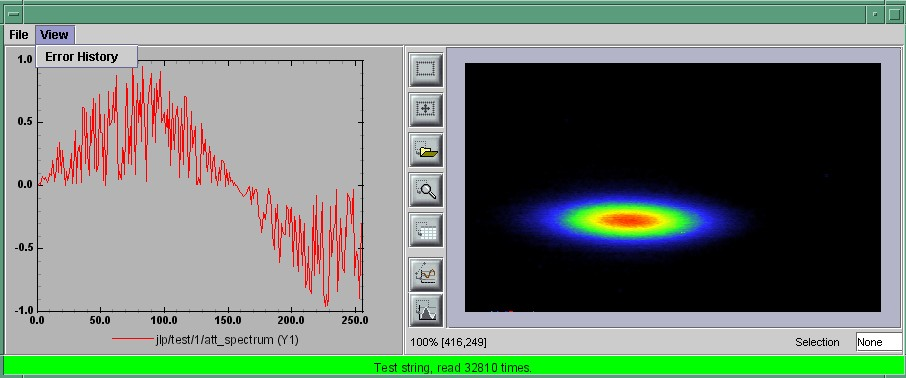
\includegraphics[scale=0.5]{atk/img/prog_guide_exple2}
\begin{minted}[linenos]{cpp}

\end{minted}

\subsubsection{Synoptic\index{Synoptic} viewer}

TangoATK provides a generic class to view and to animate the synoptics.
The name of this class is fr.esrf.tangoatk.widget.jdraw.SynopticFileViewer\index{SynopticFileViewer}.
This class is based on a ``home-made'' graphical layer called jdraw\index{jdraw}.
The jdraw package is also included inside TangoATK distribution.

SynopticFileViewer is a sub-class of the class TangoSynopticHandler.
All the work for connection to tango devices and run time animation
is done inside the TangoSynopticHandler.

The recipe for using the TangoATK synoptic viewer is the following
\begin{enumerate}
\item You use Jdraw graphical editor to draw your synoptic 
\item During drawing phase don't forget to associate parts of the drawing
to tango attributes or commands. Use the ``name'' in the property
window to do this
\item During drawing phase you can also aasociate a class (frequently a
``specific panel'' class) which will be displayed when the user
clicks on some part of the drawing. Use the ``extension'' tab in
the property window to do this.
\item Test the run-time behaviour of your synoptic. Use ``Tango Synoptic
view'' command in the ``views'' pulldown menu to do this.
\item Save the drawing file.
\item There is a simple synoptic application (SynopticAppli) which is provided
ready to use. If this generic application is enough for you, you can
forget about the step 7.
\item You can now develop a specific TangoATK based application which instantiates
the SynopticFileViewer. To load the synoptic file in the SynopticFileViewer
you have the choice : either you load it by giving the absolute path
name of the synoptic file or you load the synoptic file using Java
input streams. The second solution is used when the synoptic file
is included inside the application jarfile.
\end{enumerate}
The SynopticFilerViewer will browse the objects in the synoptic file
at run time. It discovers if some parts of the drawing is associated
with an attribute or a command. In this case it will automatically
connect to the corresponding attribute or command. Once the connection
is successfull SynopticFileViewer will animate the synoptic according
to the default behaviour described below :
\begin{itemize}
\item For \emph{tango state attributes} : the colour of the drawing object
reflects the value of the state. A mouse click on the drawing object
associated with the tango state attribute will instantiate and display
the class specified during the drawing phase. If no class is specified
the atkpanel generic device panel is displayed.
\item For \emph{tango attributes\index{attributes}} : the current value
of the attribute is displayed through the drawing object
\item For \emph{tango commands\index{commands}} : the mouse click on the
drawing object associated with the command will launch the device
command.
\item If the tooltip\index{tooltip} property is set to ``name'' when
the mouse enters \emph{any tango object} ( attribute or command),
inside the synoptic drawing the name of the tango object is displayed
in a tooltip.
\end{itemize}
The following example (ThirdApplication), is a Synoptic\index{SynopticFileViewer}\index{Synoptic}
application. We assume that the synoptic has already been drawn using
Jdraw graphical editor.


\begin{minted}[linenos]{cpp}
package examples;
import java.io.*;
import java.util.*;
import javax.swing.JFrame;
import javax.swing.JMenuItem;
import javax.swing.JMenuBar;
import javax.swing.JMenu;
import java.awt.event.ActionListener;
import java.awt.event.ActionEvent;
import java.awt.BorderLayout;
import fr.esrf.tangoatk.widget.util.ErrorHistory;
import fr.esrf.tangoatk.widget.util.ATKGraphicsUtils;
import fr.esrf.tangoatk.widget.jdraw.SynopticFileViewer;
import fr.esrf.tangoatk.widget.jdraw.TangoSynopticHandler;
public class ThirdApplication extends JFrame
{
     JMenuBar              menu;
     ErrorHistory          errorHistory;  // A window that displays errors
     SynopticFileViewer    sfv;           // TangoATK generic synoptic viewer
     
     
     public ThirdApplication()
     {
        // Swing stuff to create the menu bar and its pulldown menus
        menu = new JMenuBar();
        JMenu fileMenu = new JMenu();
        fileMenu.setText("File");   
        JMenu viewMenu = new JMenu();
        viewMenu.setText("View");
        JMenuItem quitItem = new JMenuItem();
        quitItem.setText("Quit");
        quitItem.addActionListener(new java.awt.event.ActionListener()
                                      {                 
                                       public void actionPerformed(ActionEvent evt)
                                       {quitItemActionPerformed(evt);}
                                      });
        fileMenu.add(quitItem);
        JMenuItem errorHistItem = new JMenuItem();
        errorHistItem.setText("Error History");
        errorHistItem.addActionListener(new java.awt.event.ActionListener()
                {                 
                 public void actionPerformed(ActionEvent evt)
                 {errHistItemActionPerformed(evt);}
                });
        viewMenu.add(errorHistItem);
        menu.add(fileMenu);
        menu.add(viewMenu);
        //
        // Here we create TangoATK synoptic viewer and error window.
        //
        errorHistory = new ErrorHistory();
        sfv = new SynopticFileViewer();
        try
        {
            sfv.setErrorWindow(errorHistory);
        }
        catch (Exception setErrwExcept)
        {
            System.out.println("Cannot set Error History Window");
        }

        //      
        // Here we define the name of the synoptic file to show and the tooltip mode to use
        //        
        try
        {     
          sfv.setJdrawFileName("/users/poncet/ATK_OLD/jdraw_files/id14.jdw");
          sfv.setToolTipMode (TangoSynopticHandler.TOOL_TIP_NAME);
        }
        catch (FileNotFoundException  fnfEx)
        {
           javax.swing.JOptionPane.showMessageDialog(
              null, "Cannot find the synoptic file : id14.jdw.\n"
                   + "Check the file name you entered;"
                   + " Application will abort ...\n"
                   + fnfEx,
                   "No such file",
                   javax.swing.JOptionPane.ERROR_MESSAGE);
           System.exit(-1);
        }
        catch (IllegalArgumentException  illEx)
        {
           javax.swing.JOptionPane.showMessageDialog(
              null, "Cannot parse the synoptic file : id14.jdw.\n"
                   + "Check if the file is a Jdraw file."
                   + " Application will abort ...\n"
                   + illEx,
                   "Cannot parse the file",
                   javax.swing.JOptionPane.ERROR_MESSAGE);
           System.exit(-1);
        }
        catch (MissingResourceException  mrEx)
        {
           javax.swing.JOptionPane.showMessageDialog(
              null, "Cannot parse the synoptic file : id14.jdw.\n"
                   + " Application will abort ...\n"
                   + mrEx,
                   "Cannot parse the file",
                   javax.swing.JOptionPane.ERROR_MESSAGE);
           System.exit(-1);
        }
        //
        // Add the viewers into the frame to show them
        //
        getContentPane().setLayout(new BorderLayout());
        getContentPane().add(sfv, BorderLayout.CENTER);
        //
        // add the menubar to the frame
        //
        setJMenuBar(menu);
        //
        // JFrame stuff to make the thing show.
        //
        pack();
        ATKGraphicsUtils.centerFrameOnScreen(this); //TangoATK utility to center window
        setVisible(true);
     }
     public static void main(String [] args)
     {
        new ThirdApplication();
     }
     public void quitItemActionPerformed(ActionEvent evt)
     {
        System.exit(0);
     }
     public void errHistItemActionPerformed(ActionEvent evt)
     {
        errorHistory.setVisible(true);
     }
}
[Input: line.tex]


\end{minted}
The synoptic\index{synoptic} application (ThirdApplication) should
look something like this (depending on your synoptic drawing file)\\
\\
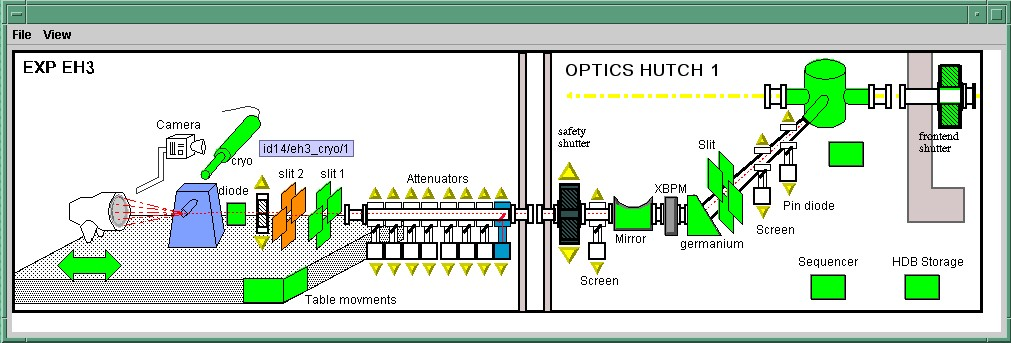
\includegraphics[scale=0.4]{atk/img/prog_guide_exple3}


\subsection{A short note on the relationship between models and viewers}

As seen in the examples above, the connection between a model\index{model}
and its viewer\index{viewer} is generally done by calling \texttt{setModel\index{setModel}(model\index{model})}
on the viewer\index{viewer}, it is never explained what happens behind
the scenes when this is done.


\subsubsection{Listeners}

Most of the viewers\index{viewer} implement some sort of \emph{listener\index{listener}}
interface, eg INumberScalarListener\index{INumberScalarListener}.
An object implementing such a listener interface has the capability
of receiving and treating \emph{events\index{event}} from a model\index{model}
which emits events.


\begin{minted}[linenos]{cpp}
// this is the setModel of a SimpleScalarViewer
  public void setModelsetModel(INumberScalar scalar) {

    clearModel();

    if (scalar != null) {
      format = scalar.getProperty("format").getPresentation();
      numberModel = scalar;
 
   // this is where the viewer connects itself to the 
   // model. After this the viewer will (hopefully) receive 
   // events through its numberScalarChange() method

   numberModel.addNumberScalarListener(this);
 
      
        numberModel.getProperty("format").addPresentationListener(this);
      numberModel.getProperty("unit").addPresentationListener(this);
    }

  }
 
 

// Each time the model of this viewer (the numberscalar attribute) decides it is time, it 
// calls the numberScalarChange method of all its registered listeners
// with a NumberScalarEvent object which contains the 
// the new value of the numberscalar attribute.
//
 
  public void numberScalarChange(NumberScalarEvent evt) {
    String val;
    val = getDisplayString(evt);
    if (unitVisible) {
      setText(val + " " + numberModel.getUnit());
    } else {
      setText(val);
    }
  }



\end{minted}


All listeners in TangoATK implement the \texttt{IErrorListener} interface
which specifies the \texttt{errorChange(ErrorEvent e)} method. This
means that all listeners are forced to handle errors in some way or
another.


\section{The key objects of TangoATK}

As seen from the examples above, the key objects of TangoATK are the
\texttt{CommandList\index{CommandList}} and the \texttt{AttributeList}\index{AttributeList}.
These two classes inherit from the abstract class \texttt{AEntityList}
which implements all of the common functionality between the two lists.
These lists use the functionality of the \texttt{CommandFactory},
the \texttt{AttributeFactory}, which both derive from \texttt{AEntityFactory,}
and the \texttt{DeviceFactory}.

In addition to these factories and lists there is one (for the time
being) other important functionality lurking around, the refreshers.


\subsection{The Refreshers}

The refreshers\index{refresher}, represented in TangoATK by the \texttt{Refresher}
object, is simply a subclass of \texttt{java.lang.Thread} which will
sleep for a given amount of time and then call a method refresh on
whatever kind of \texttt{IRefreshee} it has been given as parameter,
as shown below


\begin{minted}[linenos]{cpp}
// This is an example from DeviceFactory.
// We create a new Refresher with the name "device"
// We add ourself to it, and start the thread
 

Refresher refresher = new Refresher("device");
refresher.addRefreshee(this).start();

\end{minted}


Both the \texttt{AttributeList\index{AttributeList}} and the \texttt{DeviceFactory}
implement the \texttt{IRefreshee} interface which specify only one
method, \texttt{refresh()}, and can thus be refreshed by the \texttt{Refresher}\index{refresher}.
Even if the new release of TangoATK is based on the Tango Events\index{event}\index{Tango-Event},
the refresher mecanisme will not be removed. As a matter of fact,
the method refresh() implemented in \noun{AttributeList} skips all
attributes (members of the list) for which the subscribe\index{subscribe}
to the tango event has succeeded and calls the old refresh() method
for the others (for which subscribe to tango events has failed). 

In a first stage this will allow the TangoATK applications to mix
the use of the old tango device servers (which do not implement tango
events) and the new ones in the same code. In other words, TangoATK
subscribes for tango events if possible otherwise TangoATK will refresh
the attributes through the old refresher mecanisme.

Another reason for keeping the refresher is that the subscribe event
can fail even for the attributes of the new Tango device servers.
As soon as the specified attribute is not polled the Tango events
cannot be generated for that attribute. Therefore the event subscription
will fail. In this case the attribute will be refreshed thanks to
the ATK attribute list refresher.

The \texttt{AttributePolledList} class allows the application programmer
to force explicitly the use of the refresher method for all attributes
added in an AttributePolledList even if the corresponding device servers
implement tango events. Some viewers (fr.esrf.tangoatk.widget.attribute.Trend)
need an AttributePolledList in order to force the refresh of the attribute
without using tango events.


\subsubsection{What happens on a refresh}

When \texttt{refresh\index{refresh}} is called on the \texttt{AttributeList}
and the \texttt{DeviceFactory}, they loop through their objects, \texttt{IAttributes}
and \texttt{IDevices}, respectively, and ask them to refresh themselves
if they are not event driven.

When \noun{AttributeFactory}, creates an \texttt{IAttribute}, TangoATK
tries to subscribe for Tango Change event for that attribute. If the
subscription succeeds then the attribute is marked as event driven.
If the subscription for Tango Change event fails, TangoATK tries to
subscribe for Tango Periodic event. If the subscription succeeds then
the attribute is marked as event driven. If the subscription fails
then the attribute is marked as to be `` without events''.

In the \noun{refresh()} method of the \noun{AttributeList} during
the loop through the objects if the object is marked event driven
then the object is simply skipped. But if the object (attribute) is
not marked as event driven, the \noun{refresh()} method of the \noun{AttributeList},
asks the object to refresh itself by calling the ``\noun{refresh()}''
method of that object (attribute or device). The \noun{refresh()}
method of an attribute will in turn call the ``readAttribute'' on
the Tango device.

The result of this is that the \texttt{IAttributes} fire off events
to their registered listeners\index{listener} containing snapshots
of their state. The events are fired either because the \noun{IAttribute}
has received a Tango Change event, respectively a Tango Periodic event
(event driven objects), or because the \noun{refresh()} method of
the object has issued a readAttribute on the Tango device.


\subsection{The DeviceFactory}

The device factory is responsible for two things
\begin{enumerate}
\item Creating new devices (Tango device proxies) when needed 
\item Refreshing the state and status of these devices 
\end{enumerate}
Regarding the first point, new devices are created when they are asked
for and only if they have not already been created. If a programmer
asks for the same device twice, she is returned a reference to the
same device-object.

The \texttt{DeviceFactory} contains a Refresher as described above,
which makes sure that the all \textsf{Devices} in the \textsf{DeviceFactory}
updates their state and status and fire events to its listeners.


\subsection{The AttributeFactory and the CommandFactory}

These factories are responsible for taking a name of an attribute
or command and returning an object representing the attribute or command.
It is also responsible for making sure that the appropriate \texttt{IDevice}
is already available. Normally the programmer does not want to use
these factory classes directly. They are used by TangoATK classes
indirectly when the application programmer calls the AttributeList's
(or CommandList's) \noun{add()} method.


\subsection{The AttributeList\index{AttributeList} and the CommandList\index{CommandList}}

These lists are containers for attributes and commands. They delegate
the construction-work to the factories mentioned above, and generally
do not do much more, apart from containing refreshers, and thus being
able to make the objects they contain refresh their listeners.


\subsection{The Attributes}

The attributes\index{attributes} come in several flavors. Tango supports
the following types:
\begin{itemize}
\item Short 
\item Long 
\item Double
\item String 
\item Unsigned Char
\item Boolean
\item Unsigned Short
\item Float
\item Unsigned Long
\end{itemize}
According to Tango specifications, all these types can be of the following
formats:
\begin{itemize}
\item Scalar, a single value 
\item Spectrum, a single array 
\item Image, a two dimensional array 
\end{itemize}
For the sake of simplicity, TangoATK has combined all the numeric
types into one, presenting all of them as doubles. So the TangoATK
classes which handle the numeric attributes are : NumberScalar, NumberSpectrum
and NumberImage (Number can be short, long, double, float, ...).


\subsubsection{The hierarchy}

The numeric attribute hierarchy is expressed in the following interfaces:
\begin{description}
\item [{INumberScalar}] extends \textbf{INumber}
\item [{INumberSpectrum}] extends \textbf{INumber}
\item [{INumberImage}] extends \textbf{INumber}
\item [{\textmd{and}}] \textbf{INumber} in turn extends \textbf{IAttribute}
~
\end{description}
Each of these types emit their proper events and have their proper
listeners. Please consult the javadoc for further information.


\subsection{The Commands}

The commands\index{commands} in Tango are rather ugly beasts. There
exists the following kinds of commands
\begin{itemize}
\item Those which take input 
\item Those which do not take input 
\item Those which do output 
\item Those which do not do output 
\end{itemize}
Now, for both input and output we have the following types:
\begin{itemize}
\item Double 
\item Float
\item Unsigned Long
\item Long 
\item Unsigned Short
\item Short 
\item String
\end{itemize}
These types can appear in scalar or array formats. In addition to
this, there are also four other types of parameters:
\begin{enumerate}
\item Boolean
\item Unsigned Char Array
\item The StringLongArray 
\item The StringDoubleArray 
\end{enumerate}
The last two types mentioned above are two-dimensional arrays containing
a string array in the first dimension and a long or double array in
the second dimension, respectively.

As for the attributes, all numeric types have been converted into
doubles, but there has been made little or no effort to create an
hierarchy of types for the commands.


\subsubsection{Events\index{event} and listeners\index{listener}}

The commands publish results to their \texttt{IResultListener}s, by
the means of a \texttt{ResultEvent}. The \texttt{IResultListener}
extends \texttt{IErrorListener}, any viewer\index{viewer} of command-results
should also know how to handle errors. So a viewer of command-results
implements IResultListener interface and registers itself as a resultListener
for the command it has to show the results.
\begin{minted}[linenos]{cpp}
 


\end{minted}
\begin{center}
\label{TwoRicardo}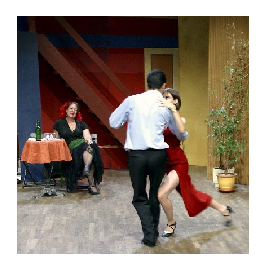
\includegraphics[scale=4]{dance/0046-reduc}
\par\end{center}


\begin{comment}
Writing a TANGO device server 
\end{comment}


\chapter{Writing a TANGO device server}


\section{The device server framework}

This chapter will present the TANGO device server framework. It will
introduce what is the device server pattern and then it will describe
a complete device server framework. A definition of classes used by
the device server framework is given in this chapter. This manual
is not intended to give the complete and detailed description of classes
data member or methods, refer to \cite{TANGO_ref_man} to get this
full description. But first, the naming convention used in this project
is detailed.

The aim of the class definition given in this chapter is only to help
the reader to understand how a TANGO device server works. For a detailed
description of these classes (and their methods), refer to chapter
\ref{Writing_chapter} or to \cite{TANGO_ref_man}.


\subsection{Naming convention and programming language}

TANGO fully supports three different programming languages which are
\textbf{C++, Java} and \textbf{Python}. This documentation focuses
on C++ Tango class. For Java and Python Tango class, have a look at
the \href{http://www.tango-controls.org}{Tango web} pages where similar
chapter for Java and Python are available.

Every software project needs a naming\index{naming} convention. The
naming convention adopted for the TDSOM is very simple and only defines
two guidelines which are:
\begin{itemize}
\item Class names start with uppercase and use capitalization for compound
words (For instance MyClassName).
\item Method names are in lowercase and use underscores for compound words
(For instance my\_method\_name).
\end{itemize}

\subsection{The device pattern}

Device server are written using the Device pattern\index{pattern}.
The aim of this pattern is to provide the control programmer with
a framework in which s/he can develop new control objects. The device
pattern uses other design patterns like the Singleton\index{singleton}
and Command patterns. These patterns are fully described in \cite{Patterns}.
The device pattern class diagram for stepper motor device is drawn
in figure \ref{Dvice pattern figure}
\begin{figure}
\begin{centering}
\subfloat[Device pattern class diagram]{

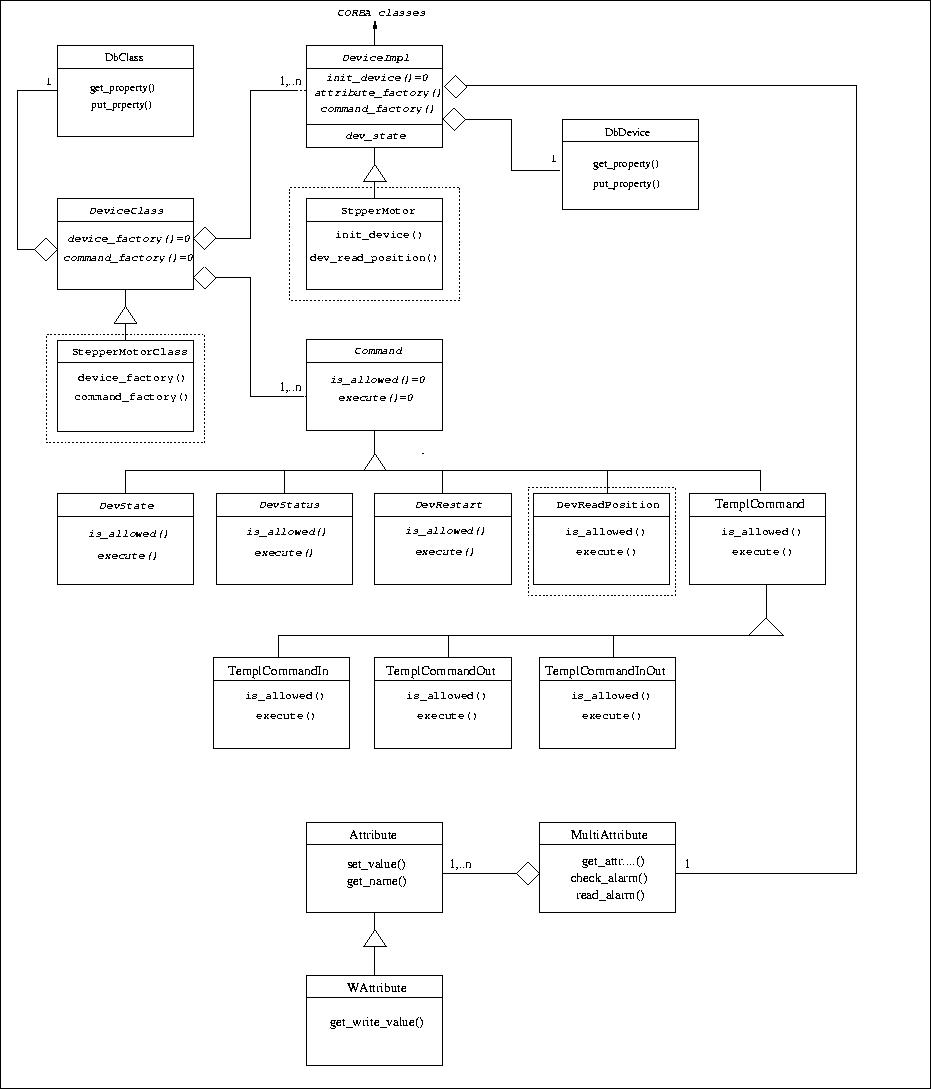
\includegraphics[width=14cm,height=18cm]{ds_writing/device_et}}
\par\end{centering}

\protect\caption{Device pattern class diagram}
\label{Dvice pattern figure}
\end{figure}
. In this figure, only classes surrounded with a dash line square
are device specific. All the other classes are part of the TDSOM core
and are developed by the Tango system team. Different kind of classes
are used by the device pattern. 
\begin{itemize}
\item Three of them are root classes and it is only necessary to inherit
from them. These classes are the \textbf{DeviceImpl}\index{DeviceImpl},
\textbf{DeviceClass\index{DeviceClass}} and \textbf{Command\index{Command}}
classes. 
\item Classes necessary to implement commands\index{command}. The TDSOM
supports two ways to create command : Using inheritance\index{inheritance}
or using the template\index{template} command model. It is possible
to mix model within the same device pattern

\begin{enumerate}
\item Using \textbf{inheritance}. This model of creating command heavily
used the polymorphism offered by each modern object oriented programming
language. In this schema, each command supported by a device via the
command\_inout\index{command-inout} or command\_inout\_async\index{command-inout-async}
operation is implemented by a separate class. The Command\index{Command}
class is the root class for each of these classes. It is an abstract
class. A \emph{execute\index{execute}} method must be defined in
each sub-class. A \emph{is\_allowed\index{is-allowed}} method may
also be re-defined in each class if the default one does not fulfill
all the needs%
\footnote{The default is\_allowed method behavior is to always allows the command%
}. In our stepper motor device server example, the DevReadPosition
command follows this model.
\item Using the \textbf{template command} model. Using this model, it is
not necessary to write one class for each command. You create one
instance of classes already defined in the TDSOM for each command.
The link between command name and method which need to be executed
is done through pointers to method. To support different kind of command,
four classes are part of the TDSOM. These classes are :

\begin{enumerate}
\item The \textbf{TemplCommand\index{TemplCommand}} class for command without
input or output parameter
\item The \textbf{TemplCommandIn\index{TemplCommandIn}} class for command
with input parameter but without output parameter
\item The \textbf{TemplCommandOu}t\index{TemplCommandOut} class for command
with output parameter but without input parameter
\item The \textbf{TemplCommandInOut\index{TemplCommandInOut}} class for
all the remaining commands
\end{enumerate}
\end{enumerate}
\item Classes necessary to implement TANGO device attributes\index{attribute}.
All these classes are part of the TANGO core classes. These classes
are the \textbf{MultiAttribute}\index{MultiAttribute}, \textbf{Attribute\index{Attribute}},
\textbf{WAttribute\index{WAttribute}}, \textbf{Attr}\index{Attr},
\textbf{SpectrumAttr\index{SpectrumAttr}} and \textbf{ImageAttr\index{ImageAttr}}
classes. The last three are used to create user attribute. Each attribute
supported by a device is implemented by a separate class. The Attr
class is the root class for each of these classes. According to the
attribute data format, the user class implementing the attribute must
inherit from the Attr, SpectrumAttr or ImageAtttr class. SpectrumAttr
class inherits from Attr class and Image Attr class inherits from
the SpectrumAttr class. The Attr base class defined three methods
called \emph{is\_allowed}\index{is-allowed}, \emph{read\index{read}}
and \emph{write}\index{write}. These methods may be redefined in
sub-classes in order to implement the attribute specific behaviour.
\item The other are device specific. For stepper motor device, they are
named StepperMotor, StepperMotorClass and DevReadPosition.
\end{itemize}

\subsubsection{The Tango base class (DeviceImpl\index{DeviceImpl} class)}


\paragraph{Description}

This class is the device root class and is the link between the Device
pattern\index{pattern} and CORBA\index{CORBA}. It inherits from
CORBA classes and implements all the methods needed to execute CORBA
operations and attributes. For instance, its method \emph{command\_inout\index{command-inout}}
is executed when a client requests a command\_inout operation. The
method \emph{name\index{name}} of the DeviceImpl class is executed
when a client requests the name CORBA attribute. This class also encapsulates
some key device data like its name\index{name}, its state\index{state},
its status\index{status}, its black box\index{black-box}.... This
class is an abstract class and cannot be instantiated as is. 


\paragraph{Contents}

The contents of this class can be summarized as :
\begin{itemize}
\item Different constructors and one destructor
\item Methods to access instance data members outside the class or its derivate
classes. These methods are necessary because data members are declared
as protected.
\item Methods triggered by CORBA attribute request
\item Methods triggered by CORBA operation\index{operation} request
\item The \emph{init\_device\index{init-device}()} method. This method
makes the class abstract. It should be implemented by a sub-class.
It is used by the inherited classes constructors.
\item Methods triggered by the automatically added State\index{State} and
Status\index{Status} commands. These methods are declared virtual
and therefore can be redefined in sub-classes. These two commands
are automatically added to the list of commands defined for a class
of devices. They are discussed in chapter \ref{Auto_cmd}
\item A method called \emph{always\_executed\_hook()\index{always-executed-hook}}
always executed for each command before the device state is tested
for command execution. This method gives the programmer a hook where
he(she) can program some mandatory action which must be done before
any command execution. An example of the such action is an hardware
access to the device to read its real hardware state.
\item A method called \emph{read\_attr\_hardware()}\index{read-attr-hardware}
triggered by the read\_attributes\index{read-attributes} CORBA operation.
This method is called once for each read\_attributes\index{read-attributes}
call. This method is virtual and may be redefined in sub-classes. 
\item A method called \emph{write\_attr\_hardware()}\index{write-attr-hardware}
triggered by the write\_attributes\index{write-attributes} CORBA
operation. This method is called once for each write\_attributes\index{write-attributes}
call. This method is virtual and may be redefined in sub-classes. 
\item Methods for signal\index{signal} management (C++ specific) 
\item Data members like the device name\index{name}, the device status\index{status},
the device state\index{state}
\item Some private methods and data members
\end{itemize}

\subsubsection{The DbDevice class}

Each DeviceImpl instance is an aggregate with one instance of the
DbDevice\index{DbDevice} class. This DbDevice class can be used to
query or modify device properties\index{properties}. It provides
an easy to use interface for device objects in the database. The description
of this class can be found in the Tango API reference documentation
available on the Tango WEB pages.


\subsubsection{The Command class}


\paragraph{Description of the inheritance\index{inheritance} model}

Within the TDSOM, each command\index{command} supported by a device
and implemented using the inheritance model is implemented by a separate
class. The Command\index{Command} class is the root class for each
of these classes. It is an abstract class. It stores the command name,
the command argument types and description and mainly defines two
methods which are the \emph{execute} and \emph{is\_allowed\index{is-allowed}}
methods. The \emph{execute\index{execute}} method should be implemented
in each sub-class. A default \emph{is\_allowed} method exists for
command always allowed. A command also stores a parameter which is
the command display type. It is also used to select if the command
must be displayed according to the application mode (every day operation
or expert mode).


\paragraph{Description of the template model}

Using this method, it is not necessary to create a separate class
for each device command. In this method, each command is represented
by an instance of one of the template\index{template} command classes.
They are four template command classes. All these classes inherits
from the Command class. These four classes are :
\begin{enumerate}
\item The \textbf{TemplCommand\index{TemplCommand}} class. One object of
this class must be created for each command without input nor output
parameters
\item The \textbf{TemplCommandIn\index{TemplCommandIn}} class. One object
of this class must be created for each command without output parameter
but with input parameter
\item The \textbf{TemplCommandOut\index{TemplCommandOut}} class. One object
of this class must be created for each command without input parameter
but with output parameter
\item The \textbf{TemplCommandInOut\index{TemplCommandInOut}} class. One
object of this class must be created for each command with input and
output parameters
\end{enumerate}
These four classes redefine the \emph{execute\index{execute}} and
\emph{is\_allowed\index{is-allowed}} method of the Command class.
These classes provides constructors which allow the user to :
\begin{itemize}
\item specify which method must be executed by these classes \emph{execute}
method
\item optionally specify which method must be executed by these classes
\emph{is\_allowed} method.
\end{itemize}
The method specification is done via pointer to method.

Remember that it is possible to mix command implementation method
within the same device pattern.


\paragraph{Contents}

The content of this class can be summarizes as :
\begin{itemize}
\item Class constructors and destructor
\item Declaration of the \emph{execute\index{execute}} method
\item Declaration of the \emph{is\_allowed\index{is-allowed}} method
\item Methods to read/set class data members
\item Methods to extract\index{extract} data from the object used to transfer
data on the network
\item Methods to insert\index{insert} data into the object used to transfer
data on the network
\item Class data members like command name, command input data type, command
input data description...
\end{itemize}

\subsubsection{The DeviceClass\index{DeviceClass} class}


\paragraph{Description}

This class implements all what is specific for a controlled object
class. For instance, every device of the same class supports the same
list of commands\index{command} and therefore, this list of available
commands is stored in this DeviceClass. The structure returned by
the info operation contains a documentation URL%
\footnote{URL stands for \textbf{U}niform \textbf{R}esource \textbf{L}ocator%
}. This documentation\index{documentation} URL\index{URL} is the
same for every device of the same class. Therefore, the documentation
URL is a data member of this class. There should have only one instance
of this class per device pattern implementation. The device list is
also stored in this class. It is an abstract class because the two
methods \emph{device\_factory\index{device-factory}()} and \emph{command\_factory\index{command-factory}()}
are declared as pure virtual. The rule of the \emph{device\_factory()}
method is to create all the devices belonging to the device class.
The rule of the \emph{command\_factory()} method is to create one
instance of all the classes needed to support device commands. This
class also stored the \emph{attribute\_factory\index{attribute-factory}}
method. The rule of this method is to store in a vector of strings,
the name of all the device attributes. This method has a default implementation
which is an empty body for device without attribute\index{attribute}.


\paragraph{Contents}

The contents of this class can be summarize as :
\begin{itemize}
\item The \emph{command\_handler\index{command-handler}} method
\item Methods to access data members.
\item Signal\index{signal} related method (C++ specific)
\item Class constructor. It is protected to implements the Singleton pattern
\item Class data members like the class command list, the device list...
\end{itemize}

\subsubsection{The DbClass\index{DbClass} class}

Each DeviceClass instance is an aggregate with one instance of the
DbClass class. This DbClass class can be used to query or modify class
properties\index{properties}. It provides an easy to use interface
for device objects in the database. The description of this class
can be found in the reference Tango C++ API documentation available
in the Tango WEB pages.


\subsubsection{The MultiAttribute\index{MultiAttribute} class}


\paragraph{Description}

This class is a container for all the TANGO attributes defined for
the device. There is one instance of this class for each device. This
class is mainly an aggregate of Attribute object(s). It has been developed
to ease TANGO attribute management.


\paragraph{Contents}

The class contents could be summarizes as :
\begin{itemize}
\item Miscellaneous methods to retrieve one attribute\index{attribute}
object in the aggregate
\item Method to retrieve a list of attribute with an alarm level defined
\item Get attribute number method
\item Miscellaneous methods to check if an attribute value is outside the
authorized limits
\item Method to add messages for all attribute with an alarm set
\item Data members with the attribute list
\end{itemize}

\subsubsection{The Attribute\index{Attribute} class}


\paragraph{Description}

There is one object of this class for each device attribute\index{attribute}.
This class is used to store all the attribute properties\index{properties},
the attribute value and all the alarm\index{alarm} related data.
Like commands, this class also stores th attribute display type. It
is foreseen to be used by future Tango graphical application toolkit
to select if the attribute must be displayed according to the application
mode (every day operation or expert mode).


\paragraph{Contents}
\begin{itemize}
\item Miscellaneous method to get boolean attribute information
\item Methods to access some data members
\item Methods to get/set attribute properties
\item Method to check if the attribute is in alarm condition
\item Methods related to attribute data
\item Friend function to print attribute properties
\item Data members (properties value and attribute data)
\end{itemize}

\subsubsection{The WAttribute\index{WAttribute} class}


\paragraph{Description}

This class inherits from the Attribute class. There is one instance
of this class for each writable\index{writable} device attribute.
On top of all the data already managed by the Attribute class, this
class stores the attribute set value.


\paragraph{Contents}

Within this class, you will mainly find methods related to attribute\index{attribute}
set value storage and some data members.


\subsubsection{The Attr class}

Within the TDSOM, each attribute\index{command} supported by a device
is implemented by a separate class. The Attr\index{Attr} class is
the root class for each of these classes. It is used in conjonction
with the Attribute and Wattribute classes to implement Tango attribute
behaviour. It defines three methods which are the \emph{is\_allowed\index{is-allowed},
read} and \emph{write} methods. A default \emph{is\_allowed} method
exists for attribute always allowed. Default \emph{read} and \emph{write}
empty methods are defined. For readable attribute, it is necessary
to overwrite the \emph{read} method. For writable attribute, it is
necessary to overwrite the \emph{write} method and for read and write
attribute, both methods must be overwritten.


\subsubsection{The SpectrumAttr\index{SpectrumAttr} class}

This class inherits from the Attr class. It is the base class for
user spectrum attribute. It is used in conjonction with the Attribute
and WAttribute class to implement Tango spectrum attribute behaviour.
From the Attr class, it inherits the Attr \emph{is\_allowed}, \emph{read}
and \emph{write} methods.


\subsubsection{The ImageAttr\index{ImageAttr} class}

This class inherits from the SpectrumAttr class. It is the base class
for user image attribute. It is used in conjonction with the Attribute
and WAttribute class to implement Tango image attribute behaviour.
From the Attr class, it inherits the Attr \emph{is\_allowed}, \emph{read}
and \emph{write} methods.


\subsubsection{The StepperMotor class}


\paragraph{Description}

This class inherits from the DeviceImpl\index{DeviceImpl} class and
is the class implementing the controlled object behavior. Each command
will trigger a method in this class written by the device server programmer
and specific to the object to be controlled. This class also stores
all the device specific data.


\paragraph{Definition}


\begin{minted}[linenos]{cpp}
1 class StepperMotor: public TANGO_BASE_CLASS
2 {
3 public :
4    StepperMotor(Tango::DeviceClass *,string &);
5    StepperMotor(Tango::DeviceClass *,const char *);
6    StepperMotor(Tango::DeviceClass *,const char *,const char *);
7    ~StepperMotor() {};
8 
9    DevLong dev_read_position(DevLong);
10   DevLong dev_read_direction(DevLong);
11   bool direct_cmd_allowed(const CORBA::Any &);
12 
13   virtual Tango::DevState dev_state();
14   virtual Tango::ConstDevString dev_status();
15 
16   virtual void always_executed_hook();
17 
18   virtual void read_attr_hardware(vector<long> &attr_list);
19   virtual void write_attr_hardware(vector<long> &attr_list);
20 
21   void read_position(Tango::Attribute &);
22   bool is_Position_allowed(Tango::AttReqType req);
23   void write_SetPosition(Tango::WAttribute &);
24   void read_Direction(Tango::Attribute &);
25 
26   virtual void init_device();
27   virtual void delete_device();
28 
29   void get_device_properties();
30 
31 protected : 
32   long axis[AGSM_MAX_MOTORS];
33   DevLong position[AGSM_MAX_MOTORS];
34   DevLong direction[AGSM_MAX_MOTORS];
35   long state[AGSM_MAX_MOTORS];
36 
37   Tango::DevLong *attr_Position_read;
38   Tango::DevLong *attr_Direction_read;
38   Tango::DevLong attr_SetPosition_write;
40 
41   Tango::DevLong min;
42   Tango::DevLong max;
43 
44   Tango::DevLong *ptr;
45 };
46 
47 } /* End of StepperMotor namespace */
\end{minted}


Line 1 : The StepperMotor class inherits from the DeviceImpl class

Line 4-7 : Class constructors and destructor

Line 9 : Method triggered by the DevReadPosition command

Line 10-11 : Methods triggered by the DevReadDirection command

Line 13 : Redefinition of the \emph{dev\_state\index{dev-state}}
method of the DeviceImpl class. This method will be triggered by the
State\index{State} command

Line 14 : Redefinition of the \emph{dev\_statu}\index{dev-status}s
method of the DeviceImpl class. This method will be triggered by the
Status\index{Status} command

Line 16 : Redefinition of the \emph{always\_executed\_hook\index{always-executed-hook}}
method.

Line 26 : Definition of the \emph{init\_device\index{init-device}}
method (declared as pure virtual by the DeviceImpl class)

Line 27 : Definition of the \emph{delete\_device}\index{delet-device}
method

Line 31-45 : Device data


\subsubsection{The StepperMotorClass class}


\paragraph{Description}

This class inherits from the DeviceClass\index{DeviceClass} class.
Like the DeviceClass class, there should be only one instance of the
StepperMotorClass. This is ensured because this class is written following
the Singleton\index{singleton} pattern as defined in \cite{Patterns}.
All controlled object class data which should be defined only once
per class must be stored in this object.


\paragraph{Definition }



     1  class StepperMotorClass : public DeviceClass

     2  \{

3  public:

     4          static StepperMotorClass {*}init(const char {*});

     5          static StepperMotorClass {*}instance();

     6          \textasciitilde{}StepperMotorClass() \{\_instance
= NULL;\}

     7          

     8  protected:

     9          StepperMotorClass(string \&);

    10          static StepperMotorClass {*}\_instance;

    11          void command\_factory();

    12          

    13  private:

    14          void device\_factory(Tango\_DevVarStringArray {*});

    15  \};



Line 1 : This class is a sub-class of the DeviceClass class

Line 4-5 and 9-10: Methods and data member necessary for the Singleton\index{singleton}
pattern

Line 6 : Class destructor

Line 11 : Definition of the \emph{command\_factor\index{command-factory}y}
method declared as pure virtual in the DeviceClass call

Line 13-14 : Definition of the \emph{device\_factory\index{device-factory}}
method declared as pure virtual in the DeviceClass class


\subsubsection{The DevReadPosition class}


\paragraph{Description}

This is the class for the DevReadPosition command. This class implements
the \emph{execute\index{execute}} and \emph{is\_allowed\index{is-allowed}}
methods defined by the Command\index{Command} class. This class is
necessary because this command is implemented using the inheritance\index{inheritance}
model.


\paragraph{Definition}


\begin{minted}[linenos]{cpp}
1  class DevReadPositionCmd : public Command
2  {
3  public:
4      DevReadPositionCmd(const char *,Tango_CmdArgType, Tango_CmdArgType, const char *, const char*);
5      ~DevReadPositionCmd() {};
6          
7      virtual bool is_allowed (DeviceImpl *, const CORBA::Any &);
8      virtual CORBA::Any *execute (DeviceImpl *, const CORBA::Any &);
9  };
\end{minted}


Line 1 : The class is a sub class of the Command class

Line 4-5 : Class constructor and destructor

Line 7-8 : Definition of the \emph{is\_allowed} and \emph{execute}
method declared as pure virtual in the Command class.


\subsubsection{The PositionAttr class}


\paragraph{Description}

This is the class for the Position attribute. This attribute is a
scalar attribute and therefore inherits from the Attr base class.
This class implements the \emph{read\index{execute}} and \emph{is\_allowed\index{is-allowed}}
methods defined by the Attr\index{Command} class.


\paragraph{Definition}


\begin{minted}[linenos]{cpp}
     1  class PositionAttr: public Tango::Attr
     2  {
     3  public:
     4     PositionAttr():Attr("Position",Tango::DEV_LONG,Tango::READ);
     5     ~PositionAttr() {};
     6          
     7     virtual void read(Tango::DeviceImpl *dev,Tango::Attribute &att)
     8     {(static_cast<StepperMotor *>(dev))->read_Position(att);}
     9     virtual bool is_allowed(Tango::DeviceImpl *dev,Tango::AttReqType ty)
    10     {return (static_cast<StepperMotor *>(dev))->is_Position_allowed(ty);}
    11  };
\end{minted}


Line 1 : The class is a sub class of the Attr class

Line 4-5 : Class constructor and destructor

Line 7 : Re-definition of the \emph{read} method defined in the Attr
class. This is simply a \textquotedbl{}forward\textquotedbl{} to the
\emph{read\_Position} method of the StepperMotor class

Line 9 : Re-definition of the \emph{is\_allowed} method defined in
the Attr class. This is also a \textquotedbl{}forward\textquotedbl{}
to the \emph{is\_Position\_allowed} method of the StepperMotor class


\subsection{Startup of a device pattern}
\label{Pattern startup}

To start the device pattern implementation for stepper motor device,
four methods of the StepperMotorClass class must be executed. These
methods are :
\begin{enumerate}
\item The creation of the StepperMethodClass singleton\index{singleton}
via its \emph{init}() method
\item The \emph{command\_factory}()\index{command-factory} method of the
StepperMotorClass class
\item The \emph{attribute\_factory}\index{attribute-factory}() method of
the StepperMotorClass class. This method has a default empty body
for device class without attributes.
\item The \emph{device\_factory}\index{device-factory}() method of the
StepperMotorClass class
\end{enumerate}
This startup procedure is described in figure \ref{pattern_startup_fig}
\begin{figure}
\begin{centering}
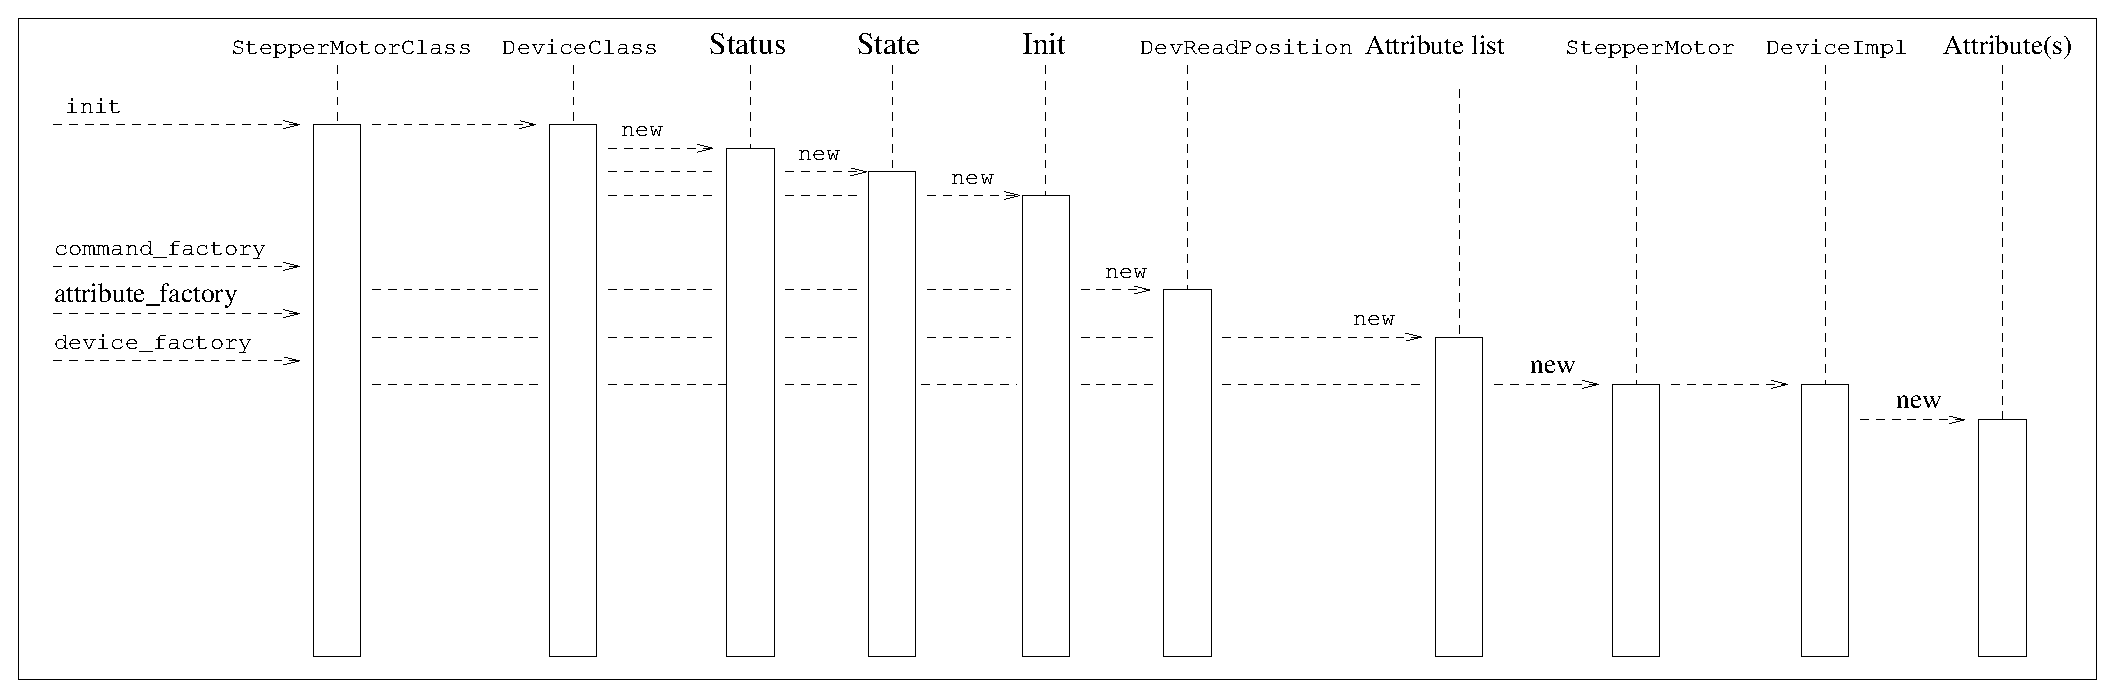
\includegraphics[width=14cm,height=10cm]{ds_writing/startup}
\par\end{centering}

\protect\caption{Device pattern startup sequence}
\label{pattern_startup_fig}
\end{figure}
 . The creation of the StepperMotorClass will automatically create
an instance of the DeviceClass class. The constructor of the DeviceClass\index{DeviceClass}
class will create the Status\index{Status}, State\index{State} and
Init\index{Init} command objects and store them in its command list.

The \emph{command\_factory}() method will simply create all the user
defined commands and add them in the command list.

The \emph{attribute\_factory}() method will simply build a list of
device attribute names.

The \emph{device\_factory}() method will create each StepperMotor
object and store them in the StepperMotorClass instance device list.
The list of devices to be created and their names is passed to the
\emph{device\_factory} method in its input argument. StepperMotor
is a sub-class of DeviceImpl class. Therefore, when a StepperMotor
object is created, a DeviceImpl object is also created. The DeviceImpl
constructor builds all the device attribute object(s) from the attribute
list built by the \emph{attribute\_factory()} method.


\subsection{Command execution sequence}

The figure \ref{command_timing_fig}
\begin{figure}[H]
\begin{centering}
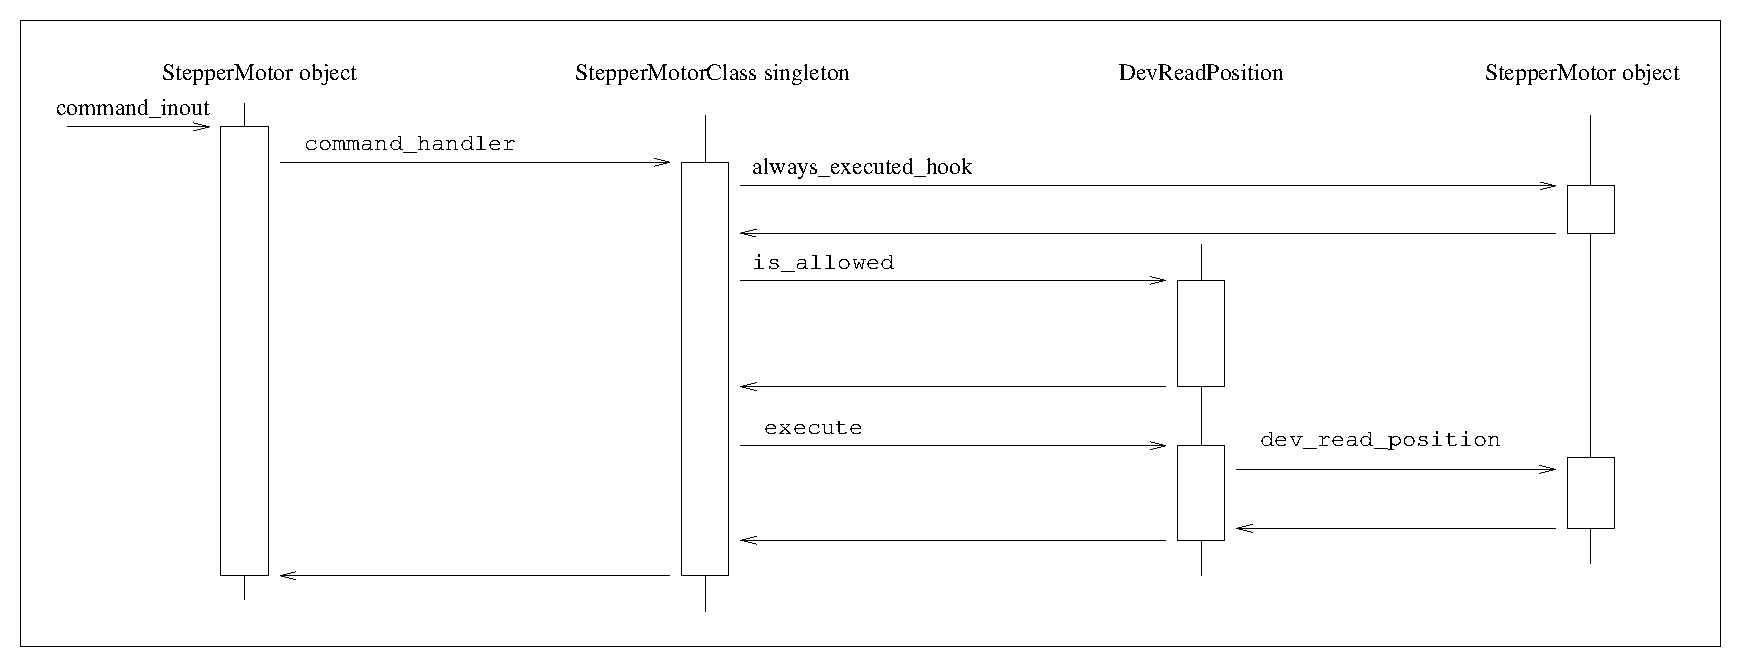
\includegraphics[width=14cm,height=8cm]{ds_writing/command}
\par\end{centering}

\protect\caption{Command execution timing}
\label{command_timing_fig}
\end{figure}
 described how the method implementing a command is executed when
a command\_inout\index{command-inout} CORBA operation is requested
by a client. The \emph{command\_inout} method of the StepperMotor
object (inherited from the DeviceImpl class) is triggered by an instance
of a class generated by the CORBA\index{CORBA} IDL compiler. This
method calls the \emph{command\_handler}()\index{command-handler}
method of the StepperMotorClass object (inherited from the DeviceClass
class). The \emph{command\_handler} method searches in its command\index{command}
list for the wanted command (using its name). If the command is found,
the \emph{always\_executed\_hook\index{always-executed-hook}} method
of the StepperMotor object is called. Then, the \emph{is\_allowed\index{is-allowed}}
method of the wanted command is executed. If the \emph{is\_allowed}
method returns correctly, the \emph{execute\index{execute}} method
is executed. The \emph{execute} method extracts the incoming data
from the CORBA object use to transmit data over the network and calls
the user written method which implements the command.


\subsection{The automatically added commands}
\label{Auto_cmd}

In order to increase the common behavior of every kind of devices
in a TANGO control system, three commands are automatically added
to each class of devices. These commands are :
\begin{itemize}
\item State\index{State}
\item Status\index{Status}
\item Init\index{Init}
\end{itemize}
The default behavior of the method called by the State command depends
on the device state. If the device state is ON or ALARM\index{ALARM},
the method will :
\begin{itemize}
\item read the attribute(s) with an alarm\index{alarm} level defined
\item check if the read value is above/below the alarm level and eventually
change the device state to ALARM.
\item returns the device state.
\end{itemize}
For all the other device state\index{state}, the method simply returns
the device state stored in the DeviceImpl class. Nevertheless, the
method used to return this state (called \emph{dev\_state}\index{state})
is defined as virtual and can be redefined in DeviceImpl sub-class.
The difference between the default State command and the state CORBA
attribute is the ability of the State\index{State} command to signal
an error to the caller by throwing an exception.

The default behavior of the method called by the Status\index{Status}
command depends on the device state. If the device state is ON or
ALARM\index{ALARM}, the method returns the device status stored in
the DeviceImpl class plus additional message(s) for all the attributes
which are in alarm condition. For all the other device state, the
method simply returns the device status as it is stored in the DeviceImpl
class. Nevertheless, the method used to return this status (called
\emph{dev\_status}\index{status}) is defined as virtual and can be
redefined in DeviceImpl sub-class. The difference between the default
Status command and the status CORBA attribute is the ability of the
Status command to signal an error to the caller by throwing an exception.

The Init\index{Init} command is used to re-initialize a device without
changing its network connection. This command calls the device \emph{delete\_device\index{delete-device}}
method and the device \emph{init\_device\index{init-device}} method.
The rule of the \emph{delete\_device} method is to free memory allocated
in the \emph{init\_device} method in order to avoid memory leak.


\subsection{Reading/Writing attributes}


\subsubsection{Reading attributes}

A Tango client is able to read Tango attribute\index{attribute}(s)
with the CORBA read\_attributes\index{read-attributes} call. Inside
the device server, this call will trigger several methods of the device
class (StepperMotor in our example) :
\begin{enumerate}
\item The \emph{always\_executed\_hook()\index{allways-executed-hook}}
method. 
\item A method call \emph{read\_attr\_hardware()}\index{read-attr-hardware}.
This method is called one time per read\_attributes CORBA call. The
aim of this method is to read the device hardware and to store the
result in a device class data member.
\item For each attribute to be read

\begin{enumerate}
\item A method called \emph{is\_<att name>\_allowed()}. The rule of this
method is to allow (or disallow) the next method to be executed. It
is usefull for device with some attributes which can be read only
in some precise conditions. It has one parameter which is the request
type (read or write)
\item A method called \emph{read\_<att name>()}. The aim of this method
is to extract the real attribute value from the hardware read-out
and to store the attribute value into the attribute object. It has
one parameter which is a reference to the Attribute object to be read.
\end{enumerate}
\end{enumerate}
The figure \ref{r_attribute_timing_fig} is a drawing of these method
calls sequencing. For attribute always readable, a default \emph{is\_allowed}
method is provided. This method always returns true.
\begin{figure}[H]
\begin{centering}
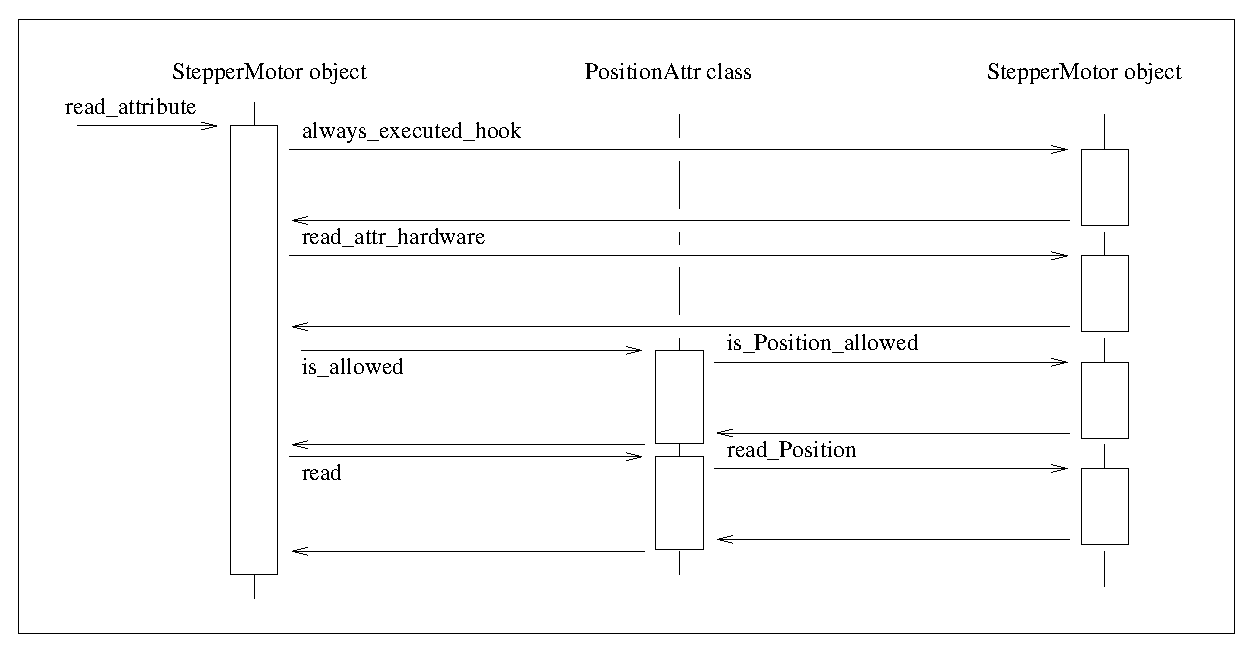
\includegraphics[scale=0.7]{ds_writing/r_attribute}
\par\end{centering}

\protect\caption{Read attribute sequencing}
\label{r_attribute_timing_fig}
\end{figure}



\subsubsection{Writing attributes}

A Tango client is able to write Tango attribute(s) with the CORBA
write\_attributes\index{write-attributes} call. Inside a device server,
this call will trigger several methods of the device class (StepperMotor
in our example)
\begin{enumerate}
\item The \emph{always\_executed\_hook()\index{allways-executed-hook}}
method. 
\item For each attribute to be written

\begin{enumerate}
\item A method called \emph{is\_<att name>\_allowed()}. The rule of this
method is to allow (or disallow) the next method to be executed. It
is usefull for device with some attributes which can be written only
in some precise conditions. It has one parameter which is the request
type (read or write)
\item A method called \emph{write\_<att name>()}. It has one parameter which
is a reference to the WAttribute object to be written. The aim of
this method is to get the data to be written from the WAttribute object
and to write this value into the corresponding hardware. If the hardware
support writing several data in one go, code the hardware access in
the \emph{write\_attr\_harware()} method.
\end{enumerate}
\item The write\_attr\_hardware()\index{write-attr-hardware} method. The
rule of this method is to effectively write the hardware in case it
is able to support writing several data in one go. If this is not
the case, don't code this method (a default implementation is coded
in the Tango base class) and code the real hardware access in each
\emph{write\_<att name>()} method.
\end{enumerate}
The figure \ref{w_attribute_timing_fig} is a drawing of these method
calls sequencing. For attribute always writeable, a default is\_allowed
method is provided. This method always allways returns true.
\begin{figure}[H]
\begin{centering}
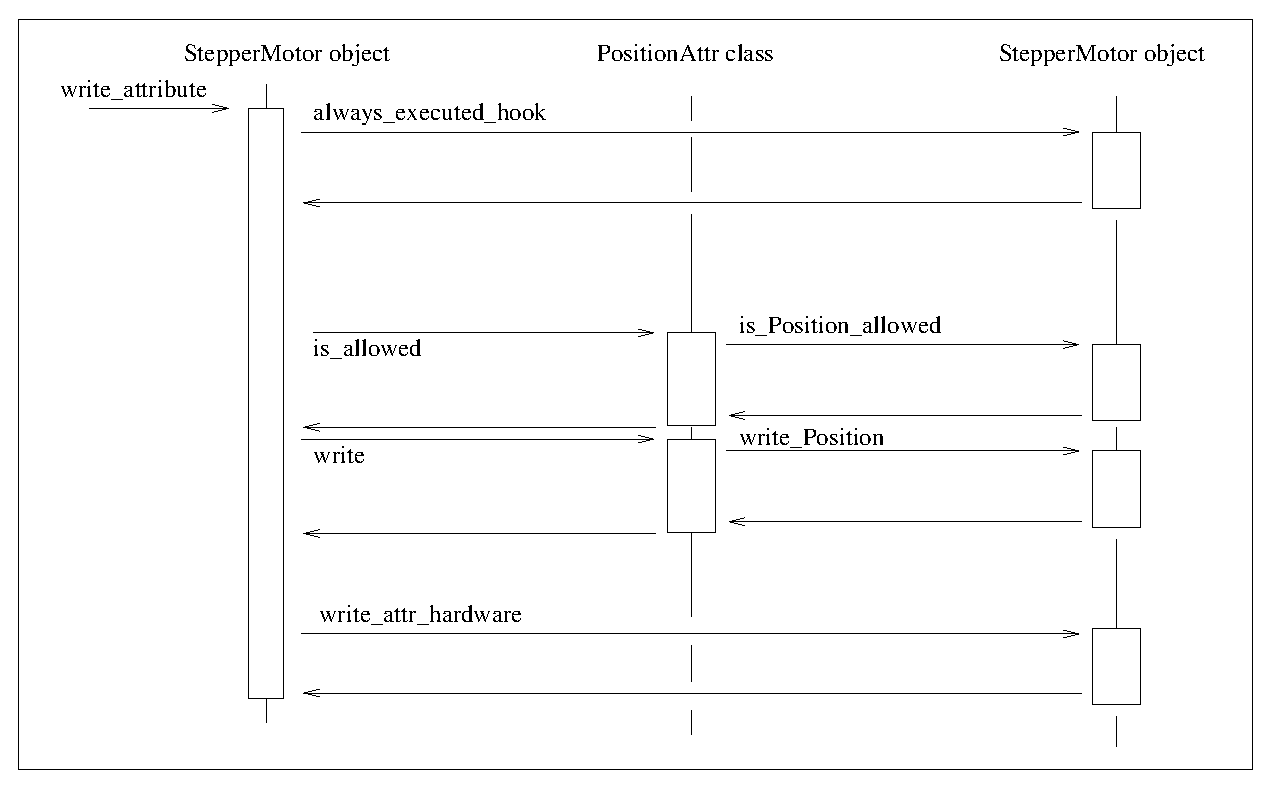
\includegraphics[scale=0.7]{ds_writing/w_attribute}
\par\end{centering}

\protect\caption{Write attribute sequencing}
\label{w_attribute_timing_fig}
\end{figure}



\subsection{The device server framework}


\subsubsection{Vocabulary}
\label{Voc}

A device server\index{server} pattern implementation is embedded
in a process called a \textbf{device server}. Several instances of
the same device server process can be used in a TANGO control system.
To identify instances, a device server process is started with an
\textbf{instance name} which is different for each instance. The device
server name is the couple device server executable\index{executable}
name/device server instance\index{instance} name. For instance, a
device server started with the following command \begin{center}Perkin
id11\end{center} starts a device server process with an instance
name id11, an executable name Perkin and a device server name Perkin/id11.


\subsubsection{The DServer class}
\label{DServer_class}

In order to simplify device server process administration, a device
of the DServer\index{DServer} class is automatically added to each
device server process. Thus, every device server process supports
the same set of administration\index{administration} commands. The
implementation of this DServer class follows the device pattern and
therefore, its device behaves like any other devices. The device name
is \begin{center}dserver/device server executable name/device server
instance name\end{center}For instance, for the device server process
described in chapter \ref{Voc}, the dserver device name is dserver/perkin/id11.
This name is returned by the adm\_name\index{adm-name} CORBA attribute
available for every device. On top of the three automatically added
commands, this device supports the following commands :
\begin{itemize}
\item DevRestart\index{DevRestart}
\item RestartServer\index{RestartServer}
\item QueryClass\index{QueryClass}
\item QueryDevice\index{QueryDevice}
\item Kill\index{Kill}
\item AddLoggingTarget (C++ server only)\index{AddLoggingTarget}
\item RemoveLoggingTarget (C++ server only)\index{RemoveLoggingTarget}
\item GetLoggingTarget (C++ server only)\index{GetLoggingTarget}
\item GetLoggingLevel (C++ server only)\index{GetLoggingLevel}
\item SetLoggingLevel (C++ server only)\index{SetLoggingLevel}
\item StopLogging (C++ server only)\index{StopLogging}
\item StartLogging (C++ server only)\index{StartLogging}
\item PolledDevice\index{PolledDevice}
\item DevPollStatus\index{DevPollStatus}
\item AddObjPolling\index{AddObjPolling}
\item RemObjPolling\index{RemObjPolling}
\item UpdObjPollingPeriod\index{UpdObjPollingPeriod}
\item StartPolling\index{StartPolling}
\item StopPolling\index{StopPolling}
\item EventSubscriptionChange\index{EventSubscriptionChange}
\item ZmqEventSubscriptionChange\index{ZmqEventSubscriptionChange}
\item LockDevice\index{LockDevice}
\item UnLockDevice\index{UnLockDevice}
\item ReLockDevices\index{ReLockDevices}
\item DevLockStatus\index{DevLockStatus}
\end{itemize}
These commands will be fully described later in this document.

Several controlled object classes can be embedded within the same
device server process and it is the rule of this device to create
all these device server patterns and to call their command and device
factories as described in \ref{Pattern startup}. The name and number
of all the classes to be created is known to this device after the
execution of a method called \emph{class\_factory}\index{class-factory}.
It is the user responsibility to write this method.


\subsubsection{The Tango::Util\index{Util} class}


\paragraph{Description}

This class merges a complete set of utilities in the same class. It
is implemented as a singleton\index{singleton} and there is only
one instance of this class per device server process. It is mandatory
to create this instance in order to run a device server. The description
of all the methods implemented in this class can be found in \cite{TANGO_ref_man}.


\paragraph{Contents}

Within this class, you can find :
\begin{itemize}
\item Static method to create/retrieve the singleton object
\item Miscellaneous utility methods like getting the server output trace
level, getting the CORBA\index{CORBA} ORB pointer, retrieving device
server instance name, getting the server PID and more. Please, refer
to \cite{TANGO_ref_man} to get a complete list of all these utility
methods.
\item Method to create the device pattern implementing the DServer class
(\emph{server\_init()}\index{server-init})
\item Method to start the server (\emph{server\_run()}\index{server-run})
\item TANGO database related methods
\end{itemize}

\subsubsection{A complete device server}

Within a complete device server, at least two implementations of the
device server pattern are created (one for the dserver object and
the other for the class of devices to control). On top of that, one
instance of the Tango::Util\index{Util} class must also be created.
\begin{figure}
\begin{centering}
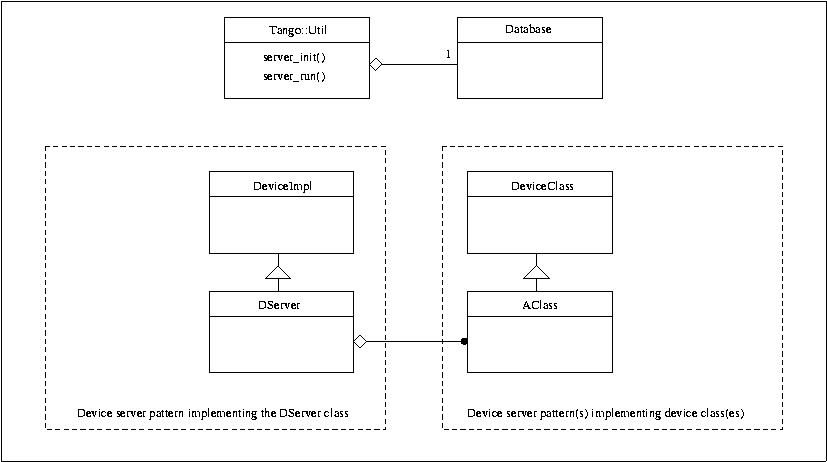
\includegraphics[width=14cm,height=10cm]{ds_writing/complete_server}
\par\end{centering}

\protect\caption{A complete device server}
\label{completeDS}
\end{figure}
 A drawing of a complete device server is in figure \ref{completeDS}


\subsubsection{Device server startup sequence}
\label{Server_startup}

The device server startup sequence is the following :
\begin{enumerate}
\item Create an instance of the Tango::Util class. This will initialize
the CORBA Object Request Broker
\item Called the \emph{server\_init\index{init}} method of the Tango::Util
instance The call to this method will :

\begin{enumerate}
\item Create the DServerClass object of the device pattern implementing
the DServer\index{DServer} class. This will create the dserver object
which during its construction will :

\begin{enumerate}
\item Called the \emph{class\_factory\index{class-factory}} method of the
DServer object. This method must create all the xxxClass instance
for all the device pattern implementation embedded in the device server
process.
\item Call the \emph{command\_factory\index{command-factory}} and \emph{device\_factory\index{device-factory}}
of all the classes previously created. The list of devices passed
to each call to the \emph{device\_factory} method is retrieved from
the TANGO database.
\end{enumerate}
\end{enumerate}
\item Wait for incoming request with the \emph{server\_run()\index{server-run}}
method of the Tango::Util class.
\end{enumerate}

\section{Exchanging data between client and server}
\label{Data exchange}

Exchanging data between clients and server means most of the time
passing data between processes running on different computer using
the network. Tango limits the type of data exchanged between client
and server and defines a way to exchange these data. This chapter
details these features. Memory allocation and error reporting are
also discussed.

\textbf{All the rules described in this chapter are valid only for
data exchanged between client and server. For device server internal
data, classical C++ types can be used.}


\subsection{Command / Attribute data types}

Commands have a fixed calling syntax - consisting of one input argument
and one output argument. Arguments type must be chosen out of a fixed
set of 24 data types. Attributes support a sub-set of these data types
(those are the data type with the (1) note) plus the DevEnum data
type. The following table details type name, code and the corresponding
CORBA IDL types.

The type name used in the type name column of this table is the C++
name. In the IDL file, all the Tango definition are grouped in a IDL\index{IDL}
module named Tango. The IDL module maps to C++ namespace\index{namespace}.
Therefore, all the data type are parts of a namespace called Tango.

\vspace{0.3cm}


\begin{center}
\begin{longtable}{|c|l|}
\hline 
Type name & IDL type\tabularnewline
\hline 
\hline 
Tango::DevBoolean (1) & boolean\tabularnewline
\hline 
Tango::DevShort (1) & short\tabularnewline
\hline 
Tango::DevEnum (2) & short (See chapter on advanced features)\tabularnewline
\hline 
Tango::DevLong (1) & long\tabularnewline
\hline 
Tango::DevLong64 (1) & long long\tabularnewline
\hline 
Tango::DevFloat (1) & float\tabularnewline
\hline 
Tango::DevDouble (1) & double\tabularnewline
\hline 
Tango::DevUShort (1) & unsigned short\tabularnewline
\hline 
Tango::DevULong (1) & unsigned long\tabularnewline
\hline 
Tango::DevULong64 (1) & unsigned long long\tabularnewline
\hline 
Tango::DevString (1) & string\tabularnewline
\hline 
Tango::DevVarCharArray & sequence of unsigned char\tabularnewline
\hline 
Tango::DevVarShortArray & sequence of short\tabularnewline
\hline 
Tango::DevVarLongArray & sequence of long\tabularnewline
\hline 
Tango::DevVarLong64Array & sequence of long long\tabularnewline
\hline 
Tango::DevVarFloatArray & sequence of float\tabularnewline
\hline 
Tango::DevVarDoubleArray & sequence of double\tabularnewline
\hline 
Tango::DevVarUShortArray & sequence of unsigned short\tabularnewline
\hline 
Tango::DevVarULongArray & sequence of unsigned long\tabularnewline
\hline 
Tango::DevVarULong64Array & sequence of unsigned long long\tabularnewline
\hline 
Tango::DevVarStringArray & sequence of string\tabularnewline
\hline 
Tango::DevVarLongStringArray & structure with a sequence of long and a sequence of string\tabularnewline
\hline 
Tango::DevVarDoubleStringArray & structure with a sequence of double and a sequence of string\tabularnewline
\hline 
Tango::DevState (1) & enumeration\tabularnewline
\hline 
Tango::DevEncoded (1) & structure with a string and a sequence of char\tabularnewline
\hline 
\end{longtable}
\par\end{center}

\vspace{0.3cm}


The CORBA Interface Definition Language uses a type called \textbf{sequence}
for variable length array. The Tango::DevUxxx types are used for unsigned
types. The Tango::DevVarxxxxArray must be used when the data to be
transferred are variable length array. The Tango::DevVarLongStringArray\index{Tango::DevVarLongStringArray}
and Tango::DevVarDoubleStringArray\index{Tango::DevVarDoubleStringArray}
are structures with two fields which are variable length array of
Tango long (32 bits) and variable length array of strings for the
Tango::DevVarLongStringArray and variable length array of double and
variable length array of string for the Tango::DevVarDoubleStringArray.
The Tango::State\index{Tango::DevState} type is used by the State\index{State}
command to return the device state. 


\subsubsection{Using data types with C++}

Unfortunately, the mapping between IDL and C++ was defined before
the C++ class library had been standardized. This explains why the
standard C++ string class or vector classes are not used in the IDL
to C++ mapping.

TANGO commands/attributes argument types can be grouped on five groups
depending on the IDL data type used. These groups are :
\begin{enumerate}
\item Data type using basic types (Tango::DevBoolean, Tango::DevShort, Tango::DevEnum,
Tango::DevLong, Tango::DevFloat, Tango::DevDouble, Tango::DevUshort
and Tango::DevULong)
\item Data type using strings (Tango::DevString type)
\item Data types using sequences\index{sequence} (Tango::DevVarxxxArray
types except Tango::DevVarLongStringArray and Tango::DevVarDoubleStringArray)
\item Data types using structures (Tango::DevVarLongStringArray and Tango::DevVarDoubleStringArray
types)
\item Data type using IDL enumeration (Tango::DevState type)
\end{enumerate}
In the following sub chapters, only summaries of the IDL to C++ mapping
are given. For a full description of the C++ mapping, please refer
to \cite{Henning}


\paragraph{Basic types}

For these types, the mapping between IDL and C++ is obvious and defined
in the following table.

\vspace{0.3cm}


\begin{center}
\begin{longtable}{|c|c|c|c|}
\hline 
Tango type name & IDL type & C++ & typedef\tabularnewline
\hline 
\hline 
Tango::DevBoolean & boolean & CORBA::Boolean & unsigned char\tabularnewline
\hline 
Tango::DevShort & short & CORBA::Short & short\tabularnewline
\hline 
Tango::DevEnum & short & CORBA::Short & \tabularnewline
\hline 
Tango::DevLong & long & CORBA::Long & int\tabularnewline
\hline 
Tango::DevLong64 & long long & CORBA::LongLong & long long or long (64 bits chip)\tabularnewline
\hline 
Tango::DevFloat & float & CORBA::Float & float\tabularnewline
\hline 
Tango::DevDouble & double & CORBA::Double & double\tabularnewline
\hline 
Tango::DevUShort & unsigned short & CORBA::UShort & unsigned short\tabularnewline
\hline 
Tango::DevULong & unsigned long & CORBA::ULong & unsigned long\tabularnewline
\hline 
Tango::DevULong64 & unsigned long long & CORBA:ULongLong & unsigned long long or unsigned long (64 bits chip)\tabularnewline
\hline 
\end{longtable}
\par\end{center}

\vspace{0.3cm}


The types defined in the column named C++ should be used for a better
portability. All these types are defined in the CORBA namespace and
therefore their qualified names is CORBA::xxx. The Tango data type
DevEnum\index{DevEnum} is a special case described in detail in the
chapter about advanced features.


\paragraph{Strings}

Strings are mapped to \textbf{char {*}}. The use of \emph{new} and
\emph{delete} for dynamic allocation of strings is not portable. Instead,
you must use helper functions defined by CORBA (in the CORBA namespace).
These functions are :


\begin{minted}[linenos]{cpp}
    char *CORBA::string_alloc(unsigned long len);
    char *CORBA::string_dup(const char *);
    void CORBA::string_free(char *);
\end{minted}


These functions handle dynamic memory for strings. The \emph{string\_alloc\index{string-alloc}}
function allocates one more byte than requested by the len parameter
(for the trailing 0). The function \emph{string\_dup\index{string-dup}}
combines the allocation and copy. Both \emph{string\_alloc} and \emph{string\_dup}
return a null pointer if allocation fails. The \emph{string\_free\index{string-free}}
function must be used to free memory allocated with \emph{string\_alloc}
and \emph{string\_dup}. Calling \emph{string\_free} for a null pointer
is safe and does nothing. The following code fragment is an example
of the Tango::DevString\index{Tango::DevString} type usage


\begin{minted}[linenos]{cpp}
     1     Tango::DevString str = CORBA::string_alloc(5);
     2     strcpy(str,"TANGO");
     3  
     4     Tango::DevString str1 = CORBA::string_dup("Do you want to danse TANGO?");
     5  
     6     CORBA::string_free(str);
     7     CORBA::string_free(str1);
\end{minted}


Line 1-2 : TANGO is a five letters string. The CORBA::string\_alloc
function parameter is 5 but the function allocates 6 bytes

Line 4 : Example of the CORBA::string\_dup function

Line 6-7 : Memory deallocation


\paragraph{Sequences}

IDL sequences\index{sequence} are mapped to C++ classes that behave
like vectors with a variable number of elements. Each IDL sequence
type results in a separate C++ class. Within each class representing
a IDL sequence types, you find the following method (only the main
methods are related here) :
\begin{enumerate}
\item Four constructors. 

\begin{enumerate}
\item A default constructor which creates an empty sequence.
\item The maximum constructor which creates a sequence with memory allocated
for at least the number of elements passed as argument. This does
not limit the number of element in the sequence but only the way how
memory is allocated to store element
\item A sophisticated constructor where it is possible to assign the memory
used by the sequence with a preallocated buffer.
\item A copy constructor which does a deep copy
\end{enumerate}
\item An assignment operator which does a deep copy
\item A \emph{length} accessor which simply returns the current number of
elements in the sequence
\item A \emph{length\index{length}} modifier which changes the length of
the sequence (which is different than the number of elements in the
sequence)
\item Overloading of the {[}{]} operator. The subscript operator {[}{]}
provides access to the sequence element. For a sequence containing
elements of type T, the {[}{]} operator is overloaded twice to return
value of type T \& and const T \&. Insertion into a sequence using
the {[}{]} operator for the const T \& make a deep copy. Sequence
are numbered between 0 and \emph{length}() -1.
\end{enumerate}
Note that using the maximum constructor will not prevent you from
setting the length of the sequence with a call to the length modifier.
The following code fragment is an example of how to use a Tango::DevVarLongArray\index{Tango::DevVarLongArray}
type


\begin{minted}[linenos]{cpp}
     1     Tango::DevVarLongArray *mylongseq_ptr;
     2     mylongseq_ptr = new Tango::DevVarLongArray();
     3     mylongseq_ptr->length(4);
     4  
     5     (*mylongseq_ptr)[0] = 1;
     6     (*mylongseq_ptr)[1] = 2;
     7     (*mylongseq_ptr)[2] = 3;
     8     (*mylongseq_ptr)[3] = 4;
     9  
    10     // (*mylongseq_ptr)[4] = 5;
    11  
    12     CORBA::Long nb_elt = mylongseq_ptr->length();
    13  
    14     mylongseq_ptr->length(5);
    15     (*mylongseq_ptr)[4] = 5;
    16  
    17     for (int i = 0;i < mylongseq_ptr->length();i++)
    18          cout << "Sequence elt " << i + 1 << " = " << (*mylongseq_ptr)[i] << endl;
\end{minted}


Line 1 : Declare a pointer to Tango::DevVarLongArray type which is
a sequence of long

Line 2 : Create an empty sequence\index{sequence}

Line 3 : Change the length\index{length} of the sequence to 4

Line 5 - 8 : Initialize sequence elements

Line 10 ; Oups !!! The length of the sequence is 4. The behavior of
this line is undefined and may be a core can be dumped at run time

Line 12 : Get the number of element actually stored in the sequence

Line 14-15 : Grow the sequence to five elements and initialize element
number 5

Line 17-18 : Print sequence element

Another example for the Tango::DevVarStringArray\index{Tango::DevVarStringArray}
type is given


\begin{minted}[linenos]{cpp}
     1     Tango::DevVarStringArray mystrseq(4);
     2     mystrseq.length(4);
     3  
     4     mystrseq[0] = CORBA::string_dup("Rock and Roll");
     5     mystrseq[1] = CORBA::string_dup("Bossa Nova");
     6     mystrseq[2] = CORBA::string_dup("Waltz");
     7     mystrseq[3] = CORBA::string_dup("Tango");
     8  
     9     CORBA::Long nb_elt = mystrseq.length();
    10  
    11     for (int i = 0;i < mystrseq.length();i++)
    12          cout << "Sequence elt " << i + 1 << " = " << mystrseq[i] << endl;
\end{minted}


Line 1 : Create a sequence using the maximum constructor

Line 2 : Set the sequence length to 4. This is mandatory even if you
used the maximum constructor.

Line 4-7 : Populate the sequence

Line 9 : Get how many strings are stored into the sequence

Line 11-12 : Print sequence elements.


\paragraph{Structures}

Only three TANGO types are defined as structures. These types are
the Tango::DevVarLongStringArray\index{Tango::DevVarLongStringArray},
the Tango::DevVarDoubleStringArray\index{Tango::DevVarDoubleStringArray}
and the Tango::DevEncoded\index{Tango::DevEncoded} data type. IDL
structures map to C++ structures with corresponding members. For the
Tango::DevVarLongStringArray, the two members are named \emph{svalue\index{svalue}}
for the sequence of strings and \emph{lvalue\index{lvalue}} for the
sequence of longs. For the Tango::DevVarDoubleStringArray, the two
structure members are called \emph{svalue} for the sequence of strings
and \emph{dvalue\index{dvalue}} for the sequence of double. For the
Tango::DevEncoded, the two structure members are called \emph{encoded\_format\index{encoded-format}}
for a string describing the data coding and \emph{encoded\_data\index{encoded-data}}
for the data themselves. The encoded\_data field type is a Tango::DevVarCharArray.
An example of the usage of the Tango::DevVarLongStringArray type is
detailed below.


\begin{minted}[linenos]{cpp}
     1     Tango::DevVarLongStringArray my_vl;
     2  
     3     myvl.svalue.length(2);
     4     myvl.svalue[0] = CORBA_string_dup("Samba");
     5     myvl.svalue[1] = CORBA_string_dup("Rumba");
     6  
     7     myvl.lvalue.length(1);
     8     myvl.lvalue[0] = 10;
\end{minted}


Line 1 : Declaration of the structure

Line 3-5 : Initialization of two strings in the sequence of string
member

Line 7-8 : Initialization of one long in the sequence of long member


\paragraph{The DevState data type}

The Tango::DevState\index{Tango::DevState} data type is used to transfer
device state between client and server. It is a IDL enumeration. IDL
enumerated types map to C++ enumerations (amazing no!) with a trailing
dummy enumerator to force enumeration to be a 32 bit type. The first
enumerator will have the value 0, the next one will have the value
1 and so on.


\begin{minted}[linenos]{cpp}
     1     Tango::DevState state;
     2  
     3     state = Tango::ON;
     4     state = Tango::FAULT;
\end{minted}



\subsection{Passing data between client and server}

In order to have one definition of the CORBA operation used to send
a command to a device whatever the command data type is, TANGO uses
CORBA IDL \textbf{any\index{any}} object. The IDL type \emph{any}
provides a universal type that can hold a value of arbitrary IDL types.
Type \emph{any} therefore allows you to send and receive values whose
types are not fixed at compile time.

Type \emph{any} is often compared to a void {*} in C. Like a pointer
to void, an \emph{any} value can denote a datum of any type. However,
there is an important difference; whereas a void {*} denotes a completely
untyped value that can be interpreted only with advance knowledge
of its type, values of type \emph{any} maintain type safety. For example,
if a sender places a string value into an \emph{any}, the receiver
cannot extract the string as a value of the wrong type. Attempt to
read the contents of an \emph{any} as the wrong type cause a run-time
error.

Internally, a value of type \emph{any} consists of a pair of values.
One member of the pair is the actual value contained inside the \emph{any}
and the other member of the pair is the type code. The type code is
a description of the value's type. The type description is used to
enforce type safety when the receiver extracts the value. Extraction
of the value succeeds only if the receiver extracts the value as a
type that matches the information in the type code.

Within TANGO, the command input and output parameters are objects
of the IDL \emph{any} type. Only insertion/extraction of all types
defined as command data types is possible into/from these \emph{any}
objects.


\subsubsection{C++ mapping for IDL any type}

The IDL any\index{any} maps to the C++ class \textbf{CORBA::Any}.
This class contains a large number of methods with mainly methods
to insert/extract data into/from the any. It provides a default constructor
which builds an any which contains no value and a type code that indicates
``no value''. Such an any must be used for command which does not
need input or output parameter. The operator \textbf{<\textcompwordmark{}<=}
is overloaded many times to insert data into an any object. The operator
\textbf{>\textcompwordmark{}>=} is overloaded many times to extract
data from an any object.


\paragraph{Inserting/Extracting TANGO basic types}

The insertion or extraction of TANGO basic types is straight forward
using the <\textcompwordmark{}<= or >\textcompwordmark{}>= operators.
Nevertheless, the Tango::DevBoolean type is mapped to a unsigned char
and other IDL types are also mapped to char C++ type (The unsigned
is not taken into account in the C++ overloading algorithm). Therefore,
it is not possible to use operator overloading for these IDL types
which map to C++ char. For the Tango::DevBoolean type, you must use
the \emph{CORBA::Any::from\_boolean} or \emph{CORBA::Any::to\_boolean}
intermediate objects defined in the CORBA::Any class.


\paragraph{Inserting/Extracting TANGO strings}

The <\textcompwordmark{}<= operator is overloaded for const char {*}
and always makes a deep copy. This deep copy is done using the CORBA::\emph{string\_dup\index{string-dup}}
function. The extraction of strings uses the >\textcompwordmark{}>=
overloaded operator. The main point is that the Any\index{any} object
retains ownership of the string, so the returned pointer points at
memory\index{memory} inside the Any. This means that you must not
deallocate the extracted string and you must treat the extracted string
as read-only.


\paragraph{Inserting/Extracting TANGO sequences}

Insertion and extraction of sequences\index{sequence} also uses the
overloaded <\textcompwordmark{}<= and >\textcompwordmark{}>= operators.
The insertion operator is overloaded twice: once for insertion by
reference and once for insertion by pointer. If you insert a value
by reference, the insertion makes a deep copy. If you insert a value
by pointer, the Any\index{any} assumes the ownership of the pointed-to
memory\index{memory}. 

Extraction is always by pointer. As with strings, you must treat the
extracted pointer as read-only and must not deallocate it because
the pointer points at memory internal to the Any.


\paragraph{Inserting/Extracting TANGO structures}

This is identical to inserting/extracting sequences.


\paragraph{Inserting/Extracting TANGO enumeration}

This is identical to inserting/extracting basic types


\begin{minted}[linenos]{cpp}
     1    CORBA::Any a;
     2    Tango::DevLong l1,l2;
     3    l1 = 2;
     4    a <<= l1;
     5    a >>= l2;
     6  
     7    CORBA::Any b;
     8    Tango::DevBoolean b1,b2;
     9    b1 = true;
    10    b <<= CORBA::Any::from_boolean(b1);
    11    b >>= CORBA::Any::to_boolean(b2);
    12  
    13    CORBA::Any s;
    14    Tango::DevString str1,str2;
    15    str1 = "I like dancing TANGO";
    16    s <<= str1;
    17    s >>= str2;
    18  
    19  //   CORBA::string_free(str2);
    20  //   a <<= CORBA::string_dup("Oups");
    21  
    22    CORBA::Any seq;
    23    Tango::DevVarFloatArray fl_arr1;
    24    fl_arr1.length(2);
    25    fl_arr1[0] = 1.0;
    26    fl_arr1[1] = 2.0;
    27    seq <<= fl_arr1;
    28    const Tango::DevVarFloatArray *fl_arr_ptr;
    29    seq >>= fl_arr_ptr;
    30  
    31  //   delete fl_arr_ptr;
\end{minted}


Line 1-5 : Insertion and extraction of Tango::DevLong type

Line 7-11 Insertion and extraction of Tango::DevBoolean type using
the CORBA::Any::from\_boolean and CORBA::Any::to\_boolean intermediate
structure

Line 13-17 : Insertion and extraction of Tango::DevString type

Line 19 : Wrong ! You should not deallocate a string extracted from
an any

Line 20 : Wrong ! Memory leak because the <\textcompwordmark{}<= operator
will do the copy. 

Line 22-29 : Insertion and extraction of Tango::DevVarxxxArray types.
This is an insertion by reference and the use of the <\textcompwordmark{}<=
operator makes a deep copy of the sequence. Therefore, after line
27, it is possible to deallocate the sequence

Line 31: Wrong.! You should not deallocate a sequence extracted from
an any


\subsubsection{The insert and extract methods of the Command class}

In order to simplify the insertion/extraction into/from Any\index{any}
objects, small helper methods have been written in the Command\index{Command}
class. The signatures of these methods are :


\begin{minted}[linenos]{cpp}
     1          void extractextract(const CORBA::Any &,<Tango type> &);
     2          CORBA::Any *insertinsert(<Tango type>);
\end{minted}


An \emph{extract} method has been written for all Tango types. These
method extract the data from the Any object passed as parameter and
throw an exception if the Any data type is incompatible with the awaiting
type. An \emph{insert} method have been written for all Tango types.
These method create an Any object, insert the data into the Any and
return a pointer to the created Any. For Tango types mapped to sequences
or structures, two \emph{insert} methods have been written: one for
the insertion from pointer and the other for the insertion from reference.
For Tango strings, two \emph{insert} methods have been written: one
for insertion from a classical Tango::DevString type and the other
from a const Tango::DevString type. The first one deallocate the memory
after the insert into the Any object. The second one only inserts
the string into the Any object. 

The previous example can be rewritten using the insert/extract helper
methods (We suppose that we can use the Command class insert/extract
methods)


\begin{minted}[linenos]{cpp}
     1    Tango::DevLong l1,l2;
     2    l1 = 2;
     3    CORBA::Any *a_ptr = insert(l1);
     4    extract(*a_ptr,l2);
     5  
     6    Tango::DevBoolean b1,b2;
     7    b1 = true;
     8    CORBA::Any *b_ptr = insert(b1);
     9    extract(*b_ptr,b2);
    10  
    11    Tango::DevString str1,str2;
    12    str1 = "I like dancing TANGO";
    13    CORBA::Any *s_ptr = insert(str1);
    14    extract(*s_ptr,str2);
    15  
    16    Tango::DevVarFloatArray fl_arr1;
    17    fl_arr1.length(2);
    18    fl_arr1[0] = 1.0;
    19    fl_arr1[1] = 2.0;
    20    insert(fl_arr1);
    21    CORBA::Any *seq_ptr = insert(fl_arr1);
    22    Tango::DevVarFloatArray *fl_arr_ptr;
    23    extract(*seq_ptr,fl_arr_ptr);
\end{minted}


Line 1-4 : Insertion and extraction of Tango::DevLong type

Line 6-9 : Insertion and extraction of Tango::DevBoolean type 

Line 11-14 : Insertion and extraction of Tango::DevString type

Line 16-23 : Insertion and extraction of Tango::DevVarxxxArray types.
This is an insertion by reference which makes a deep copy of the sequence.
Therefore, after line 20, it is possible to deallocate the sequence


\subsection{C++ memory management}

The rule described here are valid for variable length command data
types like Tango::DevString or all the Tango:: DevVarxxxxArray types.

The method executing the command must allocate the memory used to
pass data back to the client or use static memory (like buffer declares
as object data member. If necessary, the ORB will deallocate this
memory after the data have been sent to the caller. Fortunately, for
incoming data, the method have no memory\index{memory} management
responsibilities. The details about memory management given in this
chapter assume that the insert/extract methods of the Tango::Command
class are used and only the method in the device object is discussed.


\subsubsection{For string}

Example of a method receiving a Tango::DevString\index{Tango::DevString}
and returning a Tango::DevString is detailed just below


\begin{minted}[linenos]{cpp}
     1  Tango::DevString MyDev::dev_string(Tango::DevString argin)
     2  {
     3      Tango::DevString        argout;
     4  
     5      cout << "the received string is " << argin << endl;
     6          
     7      string str("Am I a good Tango dancer ?");
     8      argout = new char[str.size() + 1];
     9      strcpy(argout,str.c_str());
    10          
    11      return argout;
    12  }
\end{minted}


Note that there is no need to deallocate the memory used by the incoming
string. Memory for the outgoing string is allocated at line 8, then
it is initialized at the following line. The memory allocated at line
8 will be automatically freed by the usage of the \emph{Command::insert\index{insert}()}
method. Using this schema, memory\index{memory} is allocated/freed
each time the command is executed. For constant string length, a statically
allocated buffer can be used.


\begin{minted}[linenos]{cpp}
     1  Tango::ConstDevString MyDev::dev_string(Tango::DevString argin)
     2  {
     3      Tango::ConstDevString   argout;
     4  
     5      cout << "the received string is " << argin << endl;
     6          
     7      argout = "Hello world"; 
     8      return argout;
     9  }
\end{minted}


A Tango::ConstDevString\index{Tango::ConstDevString} data type is
used. It is not a new data Tango data type. It has been introduced
only to allows \emph{Command::insert()} method overloading. The argout
pointer is initialized at line 7 with memory statically allocated.
In this case, no memory will be freed by the \emph{Command::insert()}
method. There is also no memory\index{memory} copy in the contrary
of the previous example. A buffer defined as object data member can
also be used to set the argout pointer.


\subsubsection{For array/sequence}

Example of a method returning a Tango::DevVarLongArray\index{Tango::DevVarLongArray}
is detailed just below


\begin{minted}[linenos]{cpp}
     1  Tango::DevVarLongArray *MyDev::dev_array()
     2  {
     3      Tango::DevVarLongArray  *argout  = new Tango::DevVarLongArray();
     4                  
     5      long output_array_length = ...;
     6      argout->length(output_array_length);
     7      for (int i = 0;i < output_array_length;i++)
     8          (*argout)[i] = i;
     9  
    10      return argout;
    11  }
\end{minted}


In this case, memory is allocated at line 3 and 6. Then, the sequence\index{sequence}
is populated. The sequence is created and returned using pointer.
The \emph{Command::insert()} method will insert the sequence into
the CORBA::Any object using this pointer. Therefore, the CORBA::Any
object will take ownership of the allocated memory. It will free it
when it will be destroyed by the CORBA ORB after the data have been
sent away. It is also possible to use a statically allocated memory\index{memory}
and to avoid copying in the sequence used to returned the data. This
is explained in the following example assuming a buffer of long data
is declared as device data member and named buffer.


\begin{minted}[linenos]{cpp}
     1  Tango::DevVarLongArray *MyDev::dev_array()
     2  {
     3      Tango::DevVarLongArray  *argout;
     4                  
     5      long output_array_length = ...;
     6      argout = create_DevVarLongArray(buffer,output_array_length);
     7      return argout;
     8  }
\end{minted}


At line 3 only a pointer to a DevVarLongArray is defined. This pointer
is set at line 6 using the \emph{create\_DevVarLongArray()\index{create-DevVarLongArray}}
method. This method will create a sequence using this buffer without
memory allocation and with minimum copying. The \emph{Command::insert()}
method used here is the same than the one used in the previous example.
The sequence is created in a way that the destruction of the CORBA::Any
object in which the sequence will be inserted will not destroy the
buffer. The following create\_xxx methods are defined in the DeviceImpl
class :

\vspace{0.3cm}


\begin{center}
\begin{longtable}{|c|c|}
\hline 
Method name & data type\tabularnewline
\hline 
\hline 
create\_DevVarCharArray() & unsigned char\tabularnewline
\hline 
create\_DevVarShortArray() & short\tabularnewline
\hline 
create\_DevVarLongArray() & DevLong\tabularnewline
\hline 
create\_DevVarLong64Array() & DevLong64\tabularnewline
\hline 
create\_DevVarFloatArray() & float\tabularnewline
\hline 
create\_DevVarDoubleArray() & double\tabularnewline
\hline 
create\_DevVarUShortArray() & unsigned short\tabularnewline
\hline 
create\_DevVarULongArray() & DevULong\tabularnewline
\hline 
create\_DevVarULong64Array() & DevULong64\tabularnewline
\hline 
\end{longtable}
\par\end{center}

\vspace{0.3cm}



\subsubsection{For string array/sequence}

Example of a method returning a Tango::DevVarStringArray\index{Tango::DevVarStringArray}
is detailed just below


\begin{minted}[linenos]{cpp}
     1  Tango::DevVarStringArray *MyDev::dev_str_array()
     2  {
     3     Tango::DevVarStringArray *argout  = new Tango::DevVarStringArray();
     4  
     5     argout->length(3);
     6     (*argout)[0] = CORBA::string_dup("Rumba");
     7     (*argout)[1] = CORBA::string_dup("Waltz");
     8     string str("Jerck");
     9     (*argout)[2] = CORBA::string_dup(str.c_str());
    10     return argout;
    11  }
\end{minted}


Memory is allocated at line 3 and 5. Then, the sequence\index{sequence}
is populated at lines 6,7 and 9. The usage of the \emph{CORBA::string\_dup}
function also allocates memory. The sequence is created and returned
using pointer. The \emph{Command::insert()} method will insert the
sequence into the CORBA::Any object using this pointer. Therefore,
the CORBA::Any object will take ownership of the allocated memory.
It will free it when it will be destroyed by the CORBA ORB after the
data have been sent away. For portability reason, the ORB uses the
\emph{CORBA::string\_free\index{string-free}} function to free the
memory\index{memory} allocated for each string. This is why the corresponding
\emph{CORBA::string\_du}p\index{string-dup} or \emph{CORBA::string\_alloc}
function must be used to reserve this memory.It is also possible to
use a statically allocated memory and to avoid copying in the sequence
used to returned the data. This is explained in the following example
assuming a buffer of pointer to char is declared as device data member
and named int\_buffer.


\begin{minted}[linenos]{cpp}
     1  Tango::DevVarStringArray *DocDs::dev_str_array()
     2  {
     3     int_buffer[0] = "first";
     4     int_buffer[1] = "second";
     5  
     6     Tango::DevVarStringArray *argout;
     7     argout = create_DevVarStringArray(int_buffer,2);
     8     return argout;
     9  }
\end{minted}


The intermediate buffer is initialized with statically allocated memory
at lines 3 and 4. The returned sequence is created at line 7 with
the \emph{create\_DevVarStringArray()\index{create-DevVarStringArray}}
method. Like for classical array, the sequence is created in a way
that the destruction of the CORBA::Any\index{any} object in which
the sequence will be inserted will not destroy the buffer.


\subsubsection{For Tango composed types}

Tango supports only two composed types which are Tango::DevVarLongStringArray\index{Tango::DevVarLongStringArray}
and Tango::DevVarDoubleStringArray\index{Tango::DevVarDoubleStringArray}.
These types are translated to C++ structure with two sequences. It
is not possible to use memory statically allocated for these types.
Each structure element must be initialized as described in the previous
sub-chapters using the dynamically allocated memory case.


\subsection{Reporting errors}
\label{sub:Reporting-errors}

Tango uses the C++ try/catch plus exception\index{exception} mechanism
to report errors. Two kind of errors can be transmitted between client
and server :
\begin{enumerate}
\item CORBA system error. These exceptions are raised by the ORB and indicates
major failures (A communication failure, An invalid object reference...)
\item CORBA user exception. These kind of exceptions are defined in the
IDL file. This allows an exception to contain an arbitrary amount
of error information of arbitrary type.
\end{enumerate}
TANGO defines one user exception called \textbf{DevFailed}\index{DevFailed}.
This exception is a variable length array of \textbf{DevError\index{DevError}}
type (a sequence of DevError). The DevError type is a four fields
structure. These fields are :
\begin{enumerate}
\item A string describing the type of the error. This string replaces an
error code and allows a more easy management of include files.
\item The error severity. It is an enumeration with the three values which
are WARN, ERR or PANIC.
\item A string describing in plain text the reason of the error
\item A string describing the origin of the error\index{error}
\end{enumerate}
The Tango::DevFailed type is a sequence of DevError structures in
order to transmit to the client what is the primary error reason when
several classes are used within a command. The sequence element 0
must be the DevError structure describing the primary error. A method
called \emph{print\_exception}()\index{print-exception} defined in
the Tango::Except\index{Except} class prints the content of exception
(CORBA system exception or Tango::DevFailed exception). Some static
methods of the Tango::Except class called \emph{throw\_exception}()\index{throw-exception}
can be used to throw Tango::DevFailed exception. Some other static
methods called \emph{re\_throw\_exception()\index{re-throw-exception}}
may also be used when the user want to add a new element in the exception
sequence and re-throw the exception. Details on these methods can
be found in \cite{TANGO_ref_man}.


\subsubsection{Example of throwing exception}

This example is a piece of code from the \emph{command\_handler}()
method of the DeviceImpl class. An exception\index{exception} is
thrown to the client to indicate that the requested command is not
defined in the command list.


\begin{minted}[linenos]{cpp}
     1    TangoSys_OMemStream o;
     2                  
     3    o << "Command " << command << " not found" << ends;
     4    Tango::Except::throw_exception("API_CommandNotFound",
     5                                o.str(),
     6                                "DeviceClass::command_handler");
     7  
     8  
     9    try
    10    {
    11        .....
    12    }
    13    catch (Tango::DevFailed &e)
    14    {
    15        TangoSys_OMemStream o;
    16                  
    17        o << "Command " << command << " not found" << ends;
    18        Tango::Except::re_throw_exception(e,
    19                                  "API_CommandNotFound",
    20                                  o.str(),
    21                                  "DeviceClass::command_handler");
    22    }
\end{minted}


Line 1 : Build a memory stream. Use the TangoSys\_MemStream because
memory streams are not managed the same way between Windows and Unix

Line 3 : Build the reason string in the memory stream

Line 4-5 : Throw the exception to client using one of the \emph{throw\_exception\index{throw-exception}}
static method of the Except\index{Except} class. This throw\_exception
method used here allows the definition of the error type string, the
reason string and the origin string of the DevError structure. The
remaining DevError field (the error severity) will be set to its default
value. Note that the first and third parameters are casted to a \emph{const
char {*}}. Standard C++ defines that such a string is already a \emph{const
char {*}} but the GNU C++ compiler (release 2.95) does not use this
type inside its function overloading but rather uses a \emph{char
{*}} which leads to calling the wrong function.

Line 13-22 : Re-throw an already catched tango::DevFailed exception
with one more element in the exception sequence.


\section{The Tango Logging\index{logging} Service }
\label{The-Tango-Logging chapter}

A first introduction about this logging service has been done in chapter
\ref{sec:The-Tango-Logging}

The TANGO Logging Service (TLS) gives the user the control over how
much information is actually generated and to where it goes. In practice,
the TLS allows to select both the logging level and targets of any
device within the control system.


\subsection{Logging Targets}

The TLS implementation allows each device logging requests to print
simultaneously to multiple destinations. In the TANGO terminology,
an output destination is called a \textbf{logging target}. Currently,
targets exist for console, file and log consumer device. 

CONSOLE: logs are printed to the console (i.e. the standard output),

FILE: logs are stored in a XML file. A rolling mechanism is used to
backup the log file when it reaches a certain size (see below), 

DEVICE: logs are sent to a device implementing a well known TANGO
interface (see section \ref{sec:Tango-log-consumer} for a definition
of the log consumer interface). One implementation of a log consumer
associated to a graphical user interface is available within the Tango
package. It is called the LogViewer\index{LogViewer}.

The device's logging behavior can be control by adding and/or removing
targets.

Note : When the size of a log file (for file logging target) reaches
the so-called rolling-file-threshold (rft), it is backuped as \textquotedbl{}current\_log\_file\_name\textquotedbl{}
+ \textquotedbl{}\_1\textquotedbl{} and a new \textquotedbl{}current\_log\_file\_name\textquotedbl{}
is opened. Obviously, there is only one backup file at a time (i.e.
any existing backup is destroyed before the current log file is backuped).
The default threshold is 20 Mb, the minimum is 500 Kb and the maximum
is 1000 Mb.


\subsection{Logging Levels}

Devices can be assigned a logging level. It acts as a filter to control
the kind of information sent to the targets. Since, there are (usually)
much more low level log statements than high level statements, the
logging level also control the amount of information produced by the
device. The TLS provides the following levels (semantic is just given
to be indicative of what could be log at each level):

OFF: Nothing is logged

FATAL: A fatal error occurred. The process is about to abort

ERROR: An (unrecoverable) error occurred but the process is still
alive

WARN: An error occurred but could be recovered locally

INFO: Provides information on important actions performed

DEBUG: Generates detailed information describing the internal behavior
of a device

Levels are ordered the following way: \begin{center}DEBUG < INFO
< WARN < ERROR < FATAL < OFF\end{center}

For a given device, a level is said to be enabled if it is greater
or equal to the logging level assigned to this device. In other words,
any logging request which level is lower than the device's logging
level is ignored. 

Note: The logging level can't be controlled at target level. The device's
targets shared the same device logging level.


\subsection{Sending TANGO Logging Messages}


\subsubsection{Logging macros in C++}

The TLS provides the user with easy to use C++ macros with \emph{printf}
and \emph{stream} like syntax. For each logging level, a macro is
defined in both styles:
\begin{itemize}
\item LOG\_\{FATAL, ERROR, WARN, INFO or DEBUG\}
\item \{FATAL, ERROR, WARN, INFO or DEBUG\}\_STREAM
\end{itemize}
These macros are supposed to be used within the device's main implementation
class (i.e. the class that inherits (directly or indirectly) from
the Tango::DeviceImpl class). In this context, they produce logging
messages containing the device name. In other words, they automatically
identify the log source. Section \ref{sub:C++-logging-in} gives a
trick to log in the name of device outside its main implementation
class. Printf like example:



LOG\_DEBUG((\textquotedbl{}Msg\#\%d - Hello world\textquotedbl{},
i++));



Stream like example:



DEBUG\_STREAM <\textcompwordmark{}< \textquotedbl{}Msg\#\textquotedbl{}
<\textcompwordmark{}< i++ <\textcompwordmark{}< \textquotedbl{}- Hello
world\textquotedbl{} <\textcompwordmark{}< endl;   



These two logging requests are equivalent. Note the double parenthesis
in the printf version.


\subsubsection{C++ logging in the name of a device}
\label{sub:C++-logging-in}

A device implementation is sometimes spread over several classes.
Since all these classes implement the same device, their logging requests
should be associated with this device name. Unfortunately, the C++
logging macros can't be used because they are outside the device's
main implementation class. The Tango::LogAdapter class is a workaround
for this limitation.

Any method not member of the device's main implementation class, which
send log messages associated to a device must be a member of a class
inheriting from the Tango::LogAdapter class. Here is an example:


\begin{minted}[linenos]{cpp}
1 class MyDeviceActualImpl: public Tango::LogAdapter
2 {
3 public :
4    MyDeviceActualImpl(...,Tango::DeviceImpl *device,...)
5    :Tango::LogAdpater(device)
6    {
7          ....
8 //
9 // The following log is associated to the device passed to the constructor
10 //
11         DEBUG_STREAM << "In MyDeviceActualImpl constructor" << endl;
12 
13         ....
14    }
15 };
\end{minted}



\section{Writing a device server process}
\label{Writing_chapter}

Writing a device server can be made easier by adopting the correct
approach. This chapter will describe how to write a device server
process. It is divided into the following parts : understanding the
device, defining device commands/attributes/pipes, choosing device
state and writing the necessary classes. All along this chapter, examples
will be given using the stepper motor device server. Writing a device
server for our stepper motor example device means writing :
\begin{itemize}
\item The \emph{main} function
\item The \emph{class\_factory} method (only for C++ device server)
\item The \emph{StepperMotorClass} class
\item The \emph{DevReadPositionCmd} and \emph{DevReadDirectionCmd} classes
\item The \emph{PositionAttr}, \emph{SetPositionAttr} and \emph{DirectionAttr}
classes
\item The \emph{StepperMotor} class. 
\end{itemize}
All these functions and classes will be detailed. The stepper motor
device server described in this chapter supports 2 commands and 3
attributes which are :
\begin{itemize}
\item Command DevReadPosition implemented using the inheritance\index{inheritance}
model
\item Command DevReadDirection implemented using the template\index{template}
command model
\item Attribute Position (position of the first motor). This attribute\index{attribute}
is readable and is linked with a writable attribute (called SetPosition).
When the value of this attribute is requested by the client, the value
of the associated writable attribute is also returned.
\item Attribute SetPosition (writable attribute linked with the Position
attribute). This attribute has some properties with user defined default
value.
\item Attribute Direction (direction of the first motor)
\end{itemize}
As the reader will understand during the reading of the following
sub-chapters, the command and attributes classes (\emph{DevReadPositionCmd},
\emph{DevReadDirectionCmd}, \emph{PositionAttr}, \emph{SetPositionAttr}
and \emph{DirectionAttr}) are very simple classes. A tool called \textbf{Pogo}
has been developped to automatically generate/maintain these classes
and to write part of the code needed in the remaining one. See xx
to know more on this Pogo tool.

In order to also gives an example of how the database objects part
of the Tango device pattern could be used, our device have two properties.
These properties are of the Tango long data types and are named ``Max''
and ``Min''.


\subsection{Understanding the device}

The first step before writing a device server is to develop an understanding
of the hardware to be programmed. The Equipment Responsible should
have description of the hardware and its operating modes (manuals,
spec sheets etc.). The Equipment Responsible must also provide specifications
of what the device server should do. The Device Server Programmer
should demand an exact description of the registers, alarms, interlocks
and any timing constraints which have to be kept. It is very important
to have a good understanding of the device interfacing before starting
designing a new class. 

Once the Device Server Programmer has understood the hardware the
next important step is to define what is a logical device i.e. what
part of the hardware will be abstracted out and treated as a logical
device. In doing so the following points of the TDSOM should be kept
in mind 
\begin{itemize}
\item Each device is known and accessed by its ascii name.
\item The device is exported onto the network to be imported by applications.
\item Each device belongs to a class.
\item A list of commands exists per device.
\item Applications use the device server api to execute commands on a device. 
\end{itemize}
The above points have to be taken into account when designing the
level of device abstraction. The definition of what is a device for
a certain hardware is primarily the job of the Device Server Programmer
and the Applications Programmer but can also involve the Equipment
Responsible. The Device Server Programmer should make sure that the
Applications Programmer agrees with her definition of what is a device.

Here are some guidelines to follow while defining the level of device
abstraction - 
\begin{itemize}
\item \textbf{efficiency}, make sure that not a too fine level of device
abstraction has been chosen. If possible group as many attributes
together to form a device. Discuss this with the Applications Programmer
to find out what is efficient for her application.
\item \textbf{hardware independency}, one of the main reasons for writing
device servers is to provide the Applications Programmer with a \emph{software}
interface as opposed to a \emph{hardware} interface. Hide the hardware
structure of the device. For example if the user is only interested
in a single channel of a multichannel device then define each channel
to be a logical device. The user should not be aware of hardware addresses
or cabling details. The user is very often a scientist who has a physics-oriented
world view and not a hardware-oriented world view. Hardware independency
also has the advantage that applications are immune to hardware changes
to the device 
\item \textbf{object oriented world view}, another \emph{raison d'etre}
behind the device server model is to build up an object oriented view
of the world. The device should resemble the user's view of the object
as closely as possible. In the case of the ESRF's beam lines for example,
the devices should resemble beam line scientist's view of the machine. 
\item \textbf{atomism}, each device can be considered like an atom - is
a independent object. It should appear independent to the client even
if behind the scenes it shares some hardware or software with other
objects. This is often the case with multichannel devices where the
user would like to see each channel as a device but it is obvious
that the channels cannot be programmed completely independently. The
logical device is there to hide or make transparent this fact. If
it is impossible to send commands to one device without modifying
another device then a single device should be made out the two devices. 
\item \textbf{tailored} \emph{vs} \textbf{general}, one of the philosophies
of the TDSOM is to provide tailored solutions. For example instead
of writing one \emph{serial line} class which treats the general case
of a serial line device and leaving the device protocol to be implemented
in the client the TDSOM advocates implementing a device class which
handles the protocol of the device. This way the client only has to
know the commands of the class and not the details of the protocol.
Nothing prevents the device class from using a general purpose serial
line class if it exists of course.
\end{itemize}

\subsection{Defining device commands}

Each device has a list of commands which can be executed by the application
across the network or locally. These commands are the Application
Programmer's network knobs and dials for interacting with the device.

The list of commands to be implemented depends on the capabilities
of the hardware, the list of sensible functions which can be executed
at a distance and of course the functionality required by the application.
This implies a close collaboration between the Equipment Responsible,
Device Server Programmer and the Application Programmer.

When drawing up the list of commands particular attention should be
paid to the following points 
\begin{itemize}
\item \textbf{performance}, no single command should monopolize the device
server for a long time (a nominal value for long is one second). Commands
should be implemented in such a way that it executes immediately returning
with a response. At best try to keep command execution time down to
less than the typical overhead of an rpc call i.e. som milliseconds.
This of course is not always possible e.g. a serial line device could
require 100 milliseconds of protocol exchange. The Device Server Programmer
should find the best trade-off between the users requirements and
the devices capabilities. If a command implies a sequence of events
which could last for a long time then implement the sequence of events
in another thread - don't block the device server.
\item \textbf{robustness}, should be provided which allow the client to
recover from error conditions and or do a warm startup.
\end{itemize}

\subsubsection{Standard commands}

A minimum set of three commands exist for all devices. These commands
are 
\begin{itemize}
\item State\index{State} which returns the state of a device
\item Status\index{Status} which returns the status of the device as a
formatted ascii string
\item Init\index{Init} which re-initialize a device without changing its
network connection
\end{itemize}
These commands have already been discussed in \ref{Auto_cmd}


\subsection{Choosing device state}

The device state\index{state} is a number which reflects the availability
of the device. To simplify the coding for generic application, a predefined
set of states\index{state} are supported by TANGO. This list has
14 members which are

\vspace{0.3cm}


\begin{center}
\begin{longtable}{|c|}
\hline 
State name\tabularnewline
\hline 
\hline 
ON\tabularnewline
\hline 
OFF\tabularnewline
\hline 
CLOSE\tabularnewline
\hline 
OPEN\tabularnewline
\hline 
INSERT\tabularnewline
\hline 
EXTRACT\tabularnewline
\hline 
MOVING\tabularnewline
\hline 
STANDBY\tabularnewline
\hline 
FAULT\tabularnewline
\hline 
INIT\tabularnewline
\hline 
RUNNING\tabularnewline
\hline 
ALARM\tabularnewline
\hline 
DISABLE\tabularnewline
\hline 
UNKNOWN\tabularnewline
\hline 
\end{longtable}
\par\end{center}

\vspace{0.3cm}


The names used here have obvious meaning.


\subsection{Device server utilities to ease coding/debugging}

The device server framework supports one set of utilities to ease
the process of coding and debugging\index{debug} device server code.
This utility is :
\begin{enumerate}
\item The device server verbose\index{verbose} option
\end{enumerate}
Using this facility avoids the usage of the classical ``\#ifdef DEBUG''
style which makes code less readable.


\subsubsection{The device server verbose option}

Each device server supports a verbose\index{verbose} option called
\textbf{-v}\index{-v}. Four verbose levels are defined from 1 to
4. Level 4 is the most talkative one. If you use the -v option without
specifying level, level 4 will be assumed.

Since Tango release 3, a Tango Logging Service has been introduced
(detailed in chapter \ref{The-Tango-Logging chapter}). This -v option
set-up the logging service. If it used, it will automatically add
a \emph{console} target to all devices embedded within the device
server process. Level 1 and 2 will set the logging level to all devices
embedded within the device server to INFO. Level 3 and 4 will set
the logging\index{logging} level to all devices embedded within the
device server to DEBUG. All messages sent by the API layer are associated
to the administration device.


\subsubsection{C++ utilities to ease device server coding}

Some utilities functions have been added in the C++ release to ease
Tango device server development. These utilities allow the user to
\begin{itemize}
\item Init a C++ vector from a data of one of the Tango DevVarXXXArray data
types 
\item Init a data of one of the Tango::DevVarxxxArray data type from a C++
vector
\item Print a data of one of Tango::DevVarxxxArray data type
\end{itemize}
They mainly used the ``<\textcompwordmark{}<''\index{<<@<\textcompwordmark{}<}
operator overloading features. The following code lines are an example
of usage of these utilities.


\begin{minted}[linenos]{cpp}
     1    vector<string> v1;
     2    v1.push_back("one");
     3    v1.push_back("two");
     4    v1.push_back("three");
     5          
     6    Tango::DevVarStringArray s;
     7    s << v1;
     8    cout << s << endl;
     9  
    10    vector<string> v2;
    11    v2 << s;
    12          
    13    for (int i = 0;i < v2.size();i++)
    14       cout << "vector element = " << v2[i] << endl;
\end{minted}


Line 1-4 : Create and Init a C++ string vector

Line 7 : Init a Tango::DevVarStringArray data from the C++ vector

Line 8 : Print all the Tango::DevVarStringArray element in one line
of code.

Line 11 : Init a second empty C++ string vector with the content of
the Tango::DevVarStringArray

Line 13-14 : Print vector element\\


\textbf{Warning}: Note that due to a strange behavior of the Windows
VC++ compiler compared to other compilers, to use these utilities
with the Windows VC++ compiler, you must add the line ``using namespace
tango'' at the beginning of your source file.


\subsection{Avoiding name conflicts}

Namespace are used to avoid name conflicts. Each device pattern implementation
is defined within its own namespace\index{namespace}. The name of
the namespace is the device pattern class name. In our example, the
namespace name is \emph{StepperMotor.}


\subsection{The device server main function}

A device server main\index{main} function (or method) always follows
the same framework. It exactly implements all the action described
in chapter \ref{Server_startup}. Even if it could be always the same,
it has not been included in the library because some linkers are perturbed
by the presence of two main functions.




\begin{minted}[linenos]{cpp}
     1  #include <tango.h>
     2  
     3  int main(int argc,char *argv[])
     4  {
     5  
     6      Tango::Util *tg;
     7          
     8      try
     9      {
    10          
    11          tg = Tango::Util::init(argc,argv);
    12  
    13          tg->server_init();
    14  
    15          cout << "Ready to accept request" << endl;
    16          tg->server_run();
    17      }
    18      catch (bad_alloc)
    19      {
    20           cout << "Can't allocate memory!!!" << endl;
    21           cout << "Exiting" << endl;
    22      }
    23      catch (CORBA::Exception &e)
    24      {
    25           Tango::Except::print_exception(e);
    26                  
    27           cout << "Received a CORBA::Exception" << endl;
    28           cout << "Exiting" << endl;
    29      }
    30  
    31      tg->server_cleanup();
    32                  
    33      return(0);
    34  }
\end{minted}




Line 1 : Include the \textbf{tango.h} file. This file is a master
include file. It includes several other files. The list of files included
by tango.h can be found in \cite{TANGO_ref_man}

Line 11 : Create the instance of the Tango::Util\index{Util} class
(a singleton). Passing argc,argv to this method is mandatory because
the device server command line is checked when the Tango::Util object
is constructed.

Line 13 : Start all the device pattern creation and initialization
with the \emph{server\_init()\index{server-init}} method

Line 16 : Put the server in a endless waiting loop with the \emph{server\_run()\index{server-run}}
method. In normal case, the process should never returns from this
line.

Line 18-22 : Catch all exceptions due to memory allocation error,
display a message to the user and exit

Line 23 : Catch all standard TANGO exception which could occur during
device pattern creation and initialization

Line 25 : Print exception parameters

Line 27-28 : Print an additional message

Line 31 : Cleanup the server before exiting by calling the \emph{server\_cleanup()\index{server-cleanup}}
method.


\subsection{The DServer::class\_factory method}

As described in chapter \ref{DServer_class}, C++ device server needs
a \emph{class\_factory}() method. This method creates all the device
pattern implemented in the device server by calling their \emph{init}()\index{init}
method. The following is an example of a \emph{class\_factory\index{class-factory}}
method for a device server with one implementation of the device server
pattern for stepper motor device.


\begin{minted}[linenos]{cpp}
     1  #include <tango.h>
     2  #include <steppermotorclass.h>
     3  
     4  void Tango::DServer::class_factory()
     5  {
     6  
     7     add_class(StepperMotor::StepperMotorClass::init("StepperMotor"));
     8  
     9  }
\end{minted}


Line 1 : Include the Tango master include file

Line 2 : Include the steppermotorclass class definition file

Line 7 : Create the StepperMotorClass singleton by calling its \emph{init\index{init}}
method and stores the returned pointer into the DServer object. Remember
that all classes for the device pattern implementation for the stepper
motor class is defined within a namespace\index{namespace} called
\emph{StepperMotor}.


\subsection{Writing the StepperMotorClass class}
\label{Command fact}


\subsubsection{The class declaration file}


\begin{minted}[linenos]{cpp}
     1  #include <tango.h>
     2  
     3  namespace StepperMotor
     4  {
     5  
     6  class StepperMotorClass : public Tango::DeviceClass
     7  {
     8  public:
     9      static StepperMotorClass *init(const char *);
    10      static StepperMotorClass *instance();
    11      ~StepperMotorClass() {_instance = NULL;}
    12          
    13  protected:
    14      StepperMotorClass(string &);
    15      static StepperMotorClass *_instance;
    16      void command_factory();
    17      void attribute_factory(vector<Tango::Attr *> &);
    18          
    19  public:
    20      void device_factory(const Tango::DevVarStringArray *);
    21  };
    22  
    23  } /* End of StepperMotor namespace */
\end{minted}


Line 1 : Include the Tango master include file

Line 3 : This class is defined within the \emph{StepperMotor} namespace

Line 6 : Class StepperMotorClass inherits from Tango::DeviceClass\index{DeviceClass}

Line 9-10 : Definition of the \emph{init\index{init}} and \emph{instance\index{instance}}
methods. These methods are static and can be called even if the object
is not already constructed.

Line 11: The destructor

Line 14 : The class constructor. It is protected and can't be called
from outside the class. Only the \emph{init} method allows a user
to create an instance of this class. See \cite{Patterns} to get details
about the singleton design pattern.

Line 15 : The instance pointer. It is static in order to set it to
NULL during process initialization phase

Line 16 : Definition of the \emph{command\_factory\index{command-factory}}
method

Line 17 : Definition of the \emph{attribute\_factory\index{attribute-factory}}
method

Line 20 : Definition of the \emph{device\_factory\index{device-factory}}
method


\subsubsection{The singleton related methods}



 
\begin{minted}[linenos]{cpp}
     1  #include <tango.h>
     2  
     3  #include <steppermotor.h>
     4  #include <steppermotorclass.h>
     5  
     6  namespace StepperMotor
     7  {
     8  
     9  StepperMotorClass *StepperMotorClass::_instance = NULL;
    10  
    11  StepperMotorClass::StepperMotorClass(string &s):
    12  Tango::DeviceClass(s)
    13  {
    14      INFO_STREAM << "Entering StepperMotorClass constructor" << endl;
    15          
    16      INFO_STREAM << "Leaving StepperMotorClass constructor" << endl;
    17  }
    18  
    19  
    20  StepperMotorClass *StepperMotorClass::init(const char *name)
    21  {
    22      if (_instance == NULL)
    23      {
    24            try
    25            {
    26                 string s(name);
    27                 _instance = new StepperMotorClass(s);
    28            }
    29            catch (bad_alloc)
    30            {
    31                 throw;
    32            }               
    33      }               
    34      return _instance;
    35  }
    36  
    37  StepperMotorClass *StepperMotorClass::instance()
    38  {
    39      if (_instance == NULL)
    40      {
    41            cerr << "Class is not initialised !!" << endl;
    42            exit(-1);
    43      }
    44      return _instance;
    45  }
 
\end{minted}


Line 1-4 : include files: the Tango master include file (tango.h),
the StepperMotorClass class definition file (steppermotorclass.h)
and the StepperMotor class definition file (steppermotor.h)

Line 6 : Open the \emph{StepperMotor} namespace.

Line 9 : Initialize the static \_instance field of the StepperMotorClass
class to NULL

Line 11-18 : The class constructor. It takes an input parameter which
is the controlled device class name. This parameter is passed to the
constructor of the DeviceClass\index{DeviceClass} class. Otherwise,
the constructor does nothing except printing a message

Line 20-35 : The \emph{init\index{init}} method. This method needs
an input parameter which is the controlled device class name (StepperMotor
in this case). This method checks is the instance is already constructed
by testing the \_instance data member. If the instance is not constructed,
it creates one. If the instance is already constructed, the method
simply returns a pointer to it.

Line 37-45 : The \emph{instance} method. This method is very similar
to the \emph{init} method except that if the instance is not already
constructed. the method print a message and abort the process.

As you can understand, it is not possible to construct more than one
instance of the StepperMotorClass (it is a singleton\index{singleton})
and the \emph{init} method must be called prior to any other method.


\subsubsection{The command\_factory method}

Within our example, the stepper motor device supports two commands\index{command}
which are called DevReadPosition and DevReadDirection. These two command
takes a Tango::DevLong argument as input and output parameter. The
first command is created using the inheritance\index{inheritance}
model and the second command is created using the template\index{template}
command model.


\begin{minted}[linenos]{cpp}
     1  
     2  void StepperMotorClass::command_factory()
     3  {
     4          command_list.push_back(new DevReadPositionCmd("DevReadPosition",
     5                                                        Tango::DEV_LONG,
     6                                                        Tango::DEV_LONG,
     7                                                        "Motor number (0-7)",
     8                                                        "Motor position"));
     9                                                        
    10          command_list.push_back(
    11              new TemplCommandInOut<Tango::DevLong,Tango::DevLong>
    12                  ((const char *)"DevReadDirection",
    13                   static_cast<Tango::Lg_CmdMethPtr_Lg>
    14                          (&StepperMotor::dev_read_direction),
    15                   static_cast<Tango::StateMethPtr>
    16                          (&StepperMotor::direct_cmd_allowed))
    17                                );
    18  }
    19  
\end{minted}


Line 4 : Creation of one instance of the DevReadPositionCmd class.
The class is created with five arguments which are the command name,
the command type code for its input and output parameters and two
strings which are the command input and output parameters description.
The pointer returned by the new C++ keyword is added to the vector
of available command.

Line 10-14 : Creation of the object used for the DevReadDirection
command. This command has one input and output parameter. Therefore
the created object is an instance of the TemplCommandInOut class.
This class is a C++ template class. The first template parameter is
the command input parameter type, the second template parameter is
the command output parameter type. The second TemplCommandInOut\index{TemplCommandInOut}
class constructor parameter (set at line 13) is a pointer to the method
to be executed when the command is requested. A casting is necessary
to store this pointer as a pointer to a method of the DeviceImpl class%
\footnote{The StepperMotor class inherits from the DeviceImpl class and therefore
is a DeviceImpl%
}. The third TemplCommandInOut class constructor parameter (set at
line 15) is a pointer to the method to be executed to check if the
command is allowed. This is necessary only if the default behavior
(command always allowed) does not fulfill the needs. A casting is
necessary to store this pointer as a pointer to a method of the DeviceImpl\index{DeviceImpl}
class. When a command is created using the template command method,
the input and output parameters type are determined from the template
C++ class parameters.


\subsubsection{The device\_factory method}

The \emph{device\_factory\index{device-factory}} method has one input
parameter. It is a pointer to Tango::DevVarStringArray data which
is the device name list for this class and the instance of the device
server process. This list is fetch from the Tango database.


\begin{minted}[linenos]{cpp}
     1  void StepperMotorClass::device_factory(const Tango::_DevVarStringArray *devlist_ptr)
     2  {
     3          
     4      for (long i = 0;i < devlist_ptr->length();i++)
     5      {
     6           DEBUG_STREAM << "Device name : " << (*devlist_ptr)[i] << endl;
     7                                                  
     8           device_list.push_back(new StepperMotor(this,(*devlist_ptr)[i]));       9  
    10           if (Tango::Util::_UseDb == true)
    11                export_device(device_list.back());
    12           else
    13                export_device(device_list.back(),(*devlist_ptr[i]));
    14      }
    15  }
\end{minted}


Line 4 : A loop for each device

Line 8 : Create the device object using a StepperMotor class constructor
which needs two arguments. These two arguments are a pointer to the
StepperMotorClass instance and the device name. The pointer to the
constructed object is then added to the device list vector

Line 10-13 : Export device to the outside world using the \emph{export\_device\index{export-device}}
method of the DeviceClass class.


\subsubsection{The attribute\_factory\index{attribute-factory} method}

The rule of this method is to fulfill a vector of pointer to attributes.
A reference to this vector is passed as argument to this method.


\begin{minted}[linenos]{cpp}
     1  void StepperMotorClass::attribute_factory(vector<Tango::Attr *> &att_list)
     2  {
     3      att_list.push_back(new PositionAttr());
     4  
     5      Tango::UserDefaultAttrProp def_prop;
     6      def_prop.set_label("Set the motor position");
     7      def_prop.set_format("scientific;setprecision(4)");
     8      Tango::Attr *at = new SetPositionAttr();
     9      at->set_default_properties(def_prop);
    10      att_list.push_back(at);
    11  
    12      att_list.push_back(new DirectcionAttr());
    13  }
\end{minted}


Line 3 : Create the PositionAttr class and store the pointer to this
object into the attribute pointer vector.

Line 5-7 : Create a Tango::UserDefaultAttrProp instance and set the
label and format properties default values in this object

Line 8 : Create the SetPositionAttr attribute. 

Line 9 : Set attribute user default value with the \emph{set\_default\_properties()\index{set-default-properties}}
method of the Tango::Attr class.

Line 10 : Store the pointer to this object into the attribute pointer
vector.

Line 12 : Create the DirectionAttr class and store the pointer to
this object into the attribute pointer vector.

Please, note that in some rare case, it is necessary to add attribute
to this list during the device server life cycle. This \emph{attribute\_factory()}
method is called once during device server start-up. A method \emph{add\_attribute()}
of the DeviceImpl class allows the user to add a new attribute to
the attribute list outside of this \emph{attribute\_factory()} method.
See \cite{TANGO_ref_man} for more information on this method.


\subsection{The DevReadPositionCmd class}


\subsubsection{The class declaration file}


\begin{minted}[linenos]{cpp}
     1  #include <tango.h>
     2  
     3  namespace StepperMotor
     4  {
     5  
     6  class DevReadPositionCmd : public Tango::Command
     7  {
     8  public:
     9      DevReadPositionCmd(const char *,Tango::CmdArgType,
    10                             Tango::CmdArgType,
    11                             const char *,const char *);
    12      ~DevReadPositionCmd() {};
    13          
    14      virtual bool is_allowed (Tango::DeviceImpl *, const CORBA::Any &);
    15      virtual CORBA::Any *execute (Tango::DeviceImpl *, const CORBA::Any &);
    16  };
    17  
    18  } /* End of StepperMotor namespace */
\end{minted}


Line 1 : Include the tango master include file

Line 3 : Open the \emph{StepperMotor} namespace.

Line 6 : The DevReadPositionCmd class inherits from the Tango::Command
class

Line 9 : The constructor

Line 12 : The destructor

Line 14 : The definition of the \emph{is\_allowed\index{is-allowed}}
method. This method is not necessary if the default behavior implemented
by the default \emph{is\_allowed} method fulfill the requirements.
The default behavior is to always allows the command execution (always
return true).

Line 15: The definition of the \emph{execute\index{execute}} method


\subsubsection{The class constructor}

The class constructor does nothing. It simply invoke the Command\index{Command}
constructor by passing it its five arguments which are:
\begin{enumerate}
\item The command name
\item The command\index{command} input type code
\item The command output type code
\item The command input parameter description
\item The command output parameter description
\end{enumerate}
With this 5 parameters command class constructor, the command display
level is not specified. Therefore it is set to its default value (OPERATOR).
If the command does not have input or output parameter, it is not
possible to use the Command class constructor defined with five parameters.
In this case, the command constructor execute the Command class constructor
with three elements (class name, input type, output type) and set
the input or output parameter description fields with the \emph{set\_in\_type\_desc\index{set-in-type-desc}}
or \emph{set\_out\_type\_desc\index{set-out-type-desc}} Command class
methods. To set the command display level, it is possible to use a
6 parameters constructor or it is also possible to set it in the constructor
code with the \emph{set\_disp\_level}\index{set-disp-level} method.
Many Command class constructors are defined. See \cite{TANGO_ref_man}for
a complete list.


\subsubsection{The is\_allowed\index{is-allowed} method}

In our example, the DevReadPosition command is allowed only if the
device is in the ON state. This method receives two argument which
are a pointer to the device object on which the command must be executed
and a reference to the command input Any object. This method returns
a boolean which must be set to true if the command is allowed. If
this boolean is set to false, the DeviceClass\index{DeviceClass}
\emph{command\_handle}r\index{command-handler} method will automatically
send an exception to the caller.


\begin{minted}[linenos]{cpp}
     1  bool DevReadPositionCmd::is_allowed(Tango::DeviceImpl *device,
     2                                      const CORBA::Any &in_any)
     3  {
     4       if (device->get_state() == Tango::ON)
     5            return true;
     6       else
     7            return false;
     8  }
\end{minted}


Line 4 : Call the \emph{get\_state} method of the DeviceImpl class
which simply returns the device state

Line 5 : Authorize command if the device state is ON

Line 7 : Refuse command execution in all other cases. 


\subsubsection{The execute\index{execute} method}

This method receives two arguments which are a pointer to the device
object on which the command must be executed and a reference to the
command input Any object. This method returns a pointer to an any
object which must be initialized with the data to be returned to the
caller.


\begin{minted}[linenos]{cpp}
     1  CORBA::Any *DevReadPositionCmd::execute(
     2                          Tango::DeviceImpl *device,
     3                          const CORBA::Any &in_any)
     4  {       
     5       INFO_STREAM << "DevReadPositionCmd::execute(): arrived" << endl;
     6       Tango::DevLong motor;
     7  
     8       extract(in_any,motor);
     9       return insert(
    10          (static_cast<StepperMotor *>(device))->dev_read_position(motor));
    11  }
\end{minted}


Line 8 : Extract incoming data from the input any object using a Command
class \emph{extract} helper method. If the type of the data in the
Any object is not a Tango::DevLong, the \emph{extract\index{extract}}
method will throw an exception to the client.

Line 9 : Call the stepper motor object method which execute the DevReadPosition
command and insert the returned value into an allocated Any object.
The Any object allocation is done by the \emph{insert\index{insert}}
method which return a pointer to this Any.


\subsection{The PositionAttr class}


\subsubsection{The class declaration file}


\begin{minted}[linenos]{cpp}
     1  #include <tango.h>
     2  #include <steppermotor.h>
     3  
     4  namespace StepperMotor
     5  {
     6  
     7  
     8  class PositionAttr: public Tango::Attr
     9  {
    10  public:
    11      PositionAttr():Attr("Position",
    12                          Tango::DEV_LONG,
    13                          Tango::READ_WITH_WRITE,
    14                          "SetPosition") {};
    15      ~PositionAttr() {};
    16          
    17      virtual void read(Tango::DeviceImpl *dev,Tango::Attribute &att)
    18      {(static_cast<StepperMotor *>(dev))->read_Position(att);}
    19      virtual bool is_allowed(Tango::DeviceImpl *dev,Tango::AttReqType ty)
    20      {return (static_cast<StepperMotor *>(dev))->is_Position_allowed(ty);}
    21  };
    22  
    23  } /* End of StepperMotor namespace */
    24  
    25  #endif // _STEPPERMOTORCLASS_H
\end{minted}




Line 1-2 : Include the tango master include file and the steppermotor
class definition include file

Line 4 : Open the \emph{StepperMotor} namespace.

Line 8 : The PosiitionAttr class inherits from the Tango::Attr class

Line 11-14 : The constructor with 4 arguments

Line 15 : The destructor

Line 17 : The definition of the \emph{read} method. This method forwards
the call to a StepperMotor class method called \emph{read\_Position()}

Line 19 : The definition of the \emph{is\_allowed\index{is-allowed}}
method. This method is not necessary if the default behaviour implemented
by the default \emph{is\_allowed} method fulfills the requirements.
The default behaviour is to always allows the attribute reading (always
return true). This method forwards the call to a StepperMotor class
method called \emph{is\_Position\_allowed()}


\subsubsection{The class constructor}

The class constructor does nothing. It simply invoke the Attr\index{Attr}
constructor by passing it its four arguments which are:
\begin{enumerate}
\item The attribute name
\item The attribute data type code
\item The attribute writable type code
\item The name of the associated write attribute
\end{enumerate}
With this 4 parameters Attr class constructor, the attribute display
level is not specified. Therefore it is set to its default value (OPERATOR).
To set the attribute display level, it is possible to use in the constructor
code the \emph{set\_disp\_level}\index{set-disp-level} method. Many
Attr class constructors are defined. See \cite{TANGO_ref_man}for
a complete list.

This Position attribute is a scalar attribute. For spectrum attribute,
instead of inheriting from the Attr class, the class must inherits
from the SpectrumAttr\index{SpectrumAttr} class. Many SpectrumAttr
class constructors are defined. See \cite{TANGO_ref_man}for a complete
list.

For Image attribute, instead of inheriting from the Attr class, the
class must inherits from the ImageAttr class. Many ImageAttr\index{ImageAttr}
class constructors are defined. See \cite{TANGO_ref_man}for a complete
list. 


\subsubsection{The is\_allowed\index{is-allowed} method}

This method receives two argument which are a pointer to the device
object to which the attribute belongs to and the type of request (read
or write). In the PositionAttr class, this method simply \textquotedbl{}forwards\textquotedbl{}
the request to a method of the StepperMotor class called \emph{is\_Position\_allowed()}
passing the request type to this method. This method returns a boolean
which must be set to true if the attribute is allowed. If this boolean
is set to false, the DeviceImpl\index{DeviceImpl} read\_attribute\index{read-attribute}
method will automatically send an exception to the caller.


\subsubsection{The read\index{execute} method}

This method receives two arguments which are a pointer to the device
object to which the attribute belongs to and a reference to the corresponding
attribute object. This method \textquotedbl{}forwards\textquotedbl{}
the request to a StepperMotor class called \emph{read\_Position()}
passing it the reference on the attribute object.




\subsection{The StepperMotor class}


\subsubsection{The class declaration file}


\begin{minted}[linenos]{cpp}
1 #include <tango.h>
2 
3 #define AGSM_MAX_MOTORS 8 // maximum number of motors per device
4 
5 namespace StepperMotor
6 {
7 
8 class StepperMotor: public TANGO_BASE_CLASS
9 {
10 public :
11    StepperMotor(Tango::DeviceClass *,string &);
12    StepperMotor(Tango::DeviceClass *,const char *);
13    StepperMotor(Tango::DeviceClass *,const char *,const char *);
14    ~StepperMotor() {};
15 
16    DevLong dev_read_position(DevLong);
17    DevLong dev_read_direction(DevLong);
18    bool direct_cmd_allowed(const CORBA::Any &);
19 
20    virtual Tango::DevState dev_state();
21    virtual Tango::ConstDevString dev_status();
22 
23    virtual void always_executed_hook();
24 
25    virtual void read_attr_hardware(vector<long> &attr_list);
26    virtual void write_attr_hardware(vector<long> &attr_list);
27 
28    void read_position(Tango::Attribute &);
29    bool is_Position_allowed(Tango::AttReqType req);
30    void write_SetPosition(Tango::WAttribute &);
31    void read_Direction(Tango::Attribute &);
32 
33    virtual void init_device();
34    virtual void delete_device();
35 
36    void get_device_properties();
37 
38 protected : 
39    long axis[AGSM_MAX_MOTORS];
40    DevLong position[AGSM_MAX_MOTORS];
41    DevLong direction[AGSM_MAX_MOTORS];
42    long state[AGSM_MAX_MOTORS];
43 
44    Tango::DevLong *attr_Position_read;
45    Tango::DevLong *attr_Direction_read;
46    Tango::DevLong attr_SetPosition_write;
47 
48    Tango::DevLong min;
49    Tango::DevLong max;
50 
51    Tango::DevLong *ptr;
52 };
53 
54 } /* End of StepperMotor namespace */
\end{minted}




Line 1 : Include the Tango master include file

Line 5 : Open the \emph{StepperMotor} namespace.

Line 8 : The StepperMotor class inherits from a Tango base class

Line 11-13 : Three different object constructors

Line 14 : The destructor which calls the \emph{delete\_device()} method

Line 16 : The method to be called for the execution of the DevReadPosition
command. This method must be declared as virtual if it is needed to
redefine it in a class inheriting from StepperMotor. See chapter \ref{Inheriting}
for more details about inheriting.

Line 17 : The method to be called for the execution of the DevReadDirection
command

Line 18 : The method called to check if the execution of the DevReadDirection
command is allowed. This method is necessary because the DevReadDirection
command is created using the template command method and the default
behavior is not acceptable

Line 20 : Redefinition of the \emph{dev\_state}\index{dev-state}.
This method is used by the State\index{State} command

Line 21 : Redefinition of the \emph{dev\_status}\index{dev-status}.
This method is used by the Status\index{Status} command

Line 23 : Redefinition of the \emph{always\_executed\_hook\index{always-executed-hook}}
method. This method is the place to code mandatory action which must
be executed prior to any command.

Line 25-31 : Attribute related methods

Line 32 : Definition of the \emph{init\_device\index{init-device}}
method.

Line 33 : Definition of the \emph{delete\_device\index{delete-device}}
method

Line 35 : Definition of the \emph{get\_device\_properties} method

Line 38-50 : Data members. 

Line 43-44 : Pointers to data for readable attributes Position and
Direction

Line 45 : Data for the SetPosition attribute

Line 47-48 : Data members for the two device properties


\subsubsection{The constructors}

Three constructors are defined here. It is not mandatory to defined
three constructors. But at least one is mandatory. The three constructors
take a pointer to the StepperMotorClass instance as first parameter%
\footnote{The StepperMotorClass inherits from the DeviceClass and therefore
is a DeviceClass%
}. The second parameter is the device name as a C++ string or as a
classical pointer to char array. The third parameter necessary only
for the third form of constructor is the device description string
passed as a classical pointer to a char array.


\begin{minted}[linenos]{cpp}
1  #include <tango.h>
2  #include <steppermotor.h>
3 
4  namespace StepperMotor
5  {
6 
7  StepperMotor::StepperMotor(Tango::DeviceClass *cl,string &s)
8  :TANGO_BASE_CLASS(cl,s.c_str())
9  {
10    init_device();
11 }
12 
13 StepperMotor::StepperMotor(Tango::DeviceClass *cl,const char *s)
14 :TANGO_BASE_CLASS(cl,s)
15 {
16    init_device();
17 }
18 
19 StepperMotor::StepperMotor(Tango::DeviceClass *cl,const char *s,const char *d)
20 :TANGO_BASE_CLASS(cl,s,d)
21 {
22    init_device();
23 }
24 
25 void StepperMotor::init_device()
26 {
27    cout << "StepperMotor::StepperMotor() create " << device_name << endl;
28 
29    long i;
30 
31    for (i=0; i< AGSM_MAX_MOTORS; i++)
32    {
33       axis[i] = 0;
34       position[i] = 0;
35       direction[i] = 0;
36    }
37 
38    ptr = new Tango::DevLong[10];
39 
40    get_device_properties();
41 }
42 
43 void StepperMotor::delete_device()
44 {
45    delete [] ptr;
46 }
\end{minted}


Line 1-2 : Include the Tango master include file (tango.h) and the
StepperMotor class definition file (steppermotor.h)

Line 4 : Open the \emph{StepperMotor} namespace

Line 7-11 : The first form of the class constructor. It execute the
Tango base class constructor with the two parameters. Note that the
device name passed to this constructor as a C++ string is passed to
the Tango::DeviceImpl\index{DeviceImpl} constructor as a classical
C string. Then the \emph{init\_device\index{init-device}} method
is executed.

Line 13-17 : The second form of the class constructor. It execute
the Tango base class constructor with its two parameters. Then the
\emph{init\_device} method is executed.

Line 19-23: The third form of constructor. Again, it execute the Tango
base class constructor with its three parameters. Then the \emph{init\_device}
method is executed.

Line 25-41 : The \emph{init\_device\index{init-device}} method. All
the device data initialization is done in this method. The device
properties are also retrieved from database with a call to the \emph{get\_device\_properties}
method at line 40. The device data member called \emph{ptr} is initialized
with allocated memory at line 38. It is not needed to have this pointer,
it has been added only for educational purpose.

Line 43-46 : The \emph{delete\_device\index{delete-device}} method.
The rule of this method is to free memory allocated in the \emph{init\_device}
method. In our case , only the device data member \emph{ptr} is allocated
in the \emph{init\_device} method. Therefore, its memory is freed
at line 45. This method is called by the automatically added Init
command before it calls the \emph{init\_device} method. It is also
called by the device destructor.


\subsubsection{The methods used for the DevReadDirection command}

The DevReadDirection command is created using the template command
method. Therefore, there is no specific class needed for this command
but only one object of the TemplCommandInOut class. This command needs
two methods which are the \emph{dev\_read\_direction} method and the
\emph{direct\_cmd\_allowed} method. The \emph{direct\_cmd\_allowed}
method defines here implements exactly the same behavior than the
default one. This method has been used only for pedagogic issue. The
\emph{dev\_read\_direction} method will be executed by the \emph{execute}
method of the TemplCommandInOut\index{TemplCommandInOut} class. The
\emph{direct\_cmd\_allowed} method will be executed by the \emph{is\_allowed}
method of the TemplCommandInOut class.


\begin{minted}[linenos]{cpp}
     1  DevLong StepperMotor::dev_read_direction(DevLong axis)
     2  {
     3     if (axis < 0 || axis > AGSM_MAX_MOTORS)
     4     {
     5         WARNING_STREAM << "Steppermotor::dev_read_direction(): axis out of range !";
     6         WARNING_STREAM << endl;
     7         TangoSys_OMemStream o;
     8                  
     9         o << "Axis number " << axis << " out of range" << ends;
    10         throw_exception("StepperMotor_OutOfRange",
    11                         o.str(),
    12                         "StepperMotor::dev_read_direction");
    13      }
    14  
    15      return direction[axis];
    16  }
    17  
    18  
    19  bool StepperMotor::direct_cmd_allowed(const CORBA::Any &in_data)
    20  {
    21      INFO_STREAM << "In direct_cmd_allowed() method" << endl;
    22          
    23      return true;
    24  }
    25  
\end{minted}


Line 1-16 : The \emph{dev\_read\_direction} method

Line 5-12 : Throw exception to client if the received axis number
is out of range

Line 7 : A TangoSys\_OMemStream is used as stream. The TangoSys\_OMemStream
has been defined in improve portability across platform. For Unix
like operating system, it is a ostrtream type. For operating system
with a full implementation of the standard library, it is a ostringstream
type.

Line 19-24 : The \emph{direct\_cmd\_allowed} method. The command input
data is passed to this method in case of it is needed to take the
decision. This data is still packed into the CORBA Any object.


\subsubsection{The methods used for the Position attribute}

To enable reading of attributes\index{attribute}, the StepperMotor
class must re-define two or three methods called \emph{read\_attr\_hardware\index{read-attr-hardware}(),
read\_<Attribute\_name>()\index{read-Position}} and if necessary
a method called \\
\emph{is\_<Attribute\_name>\_allowed().} The aim of the first one
is to read the hardware. It will be called only once at the beginning
of each read\_attribute CORBA call. The second method aim is to build
the exact data for the wanted attribute and to store this value into
the Attribute object. Special care has been taken in order to minimize
the number of data copy and allocation. The data passed to the Attribute
object as attribute value is passed using pointers. It must be allocated
by the method%
\footnote{It can also be data declared as object data members or memory declared
as static%
} and the Attribute\index{Attribute} object will not free this memory.
Data members called attr\_<Attribute\_name>\_read are foreseen for
this usage. The \emph{read\_attr\_hardware()} method receives a vector
of long which are indexes into the main attributes vector of the attributes
to be read. The \emph{read\_Position()} method receives a reference
to the Attribute object. The third method (\emph{is\_Position\_allowed()})
aim is to allow or dis-allow, the attribute reading. In some cases,
some attributes can be read only if some conditions are met. If this
method returns true, the \emph{read\_<Attribute\_name>()} method will
be called. Otherwise, an error will be generated for the attribute.
This method receives one argument which is an emumeration describing
the attribute request type (read or write). In our example, the reading
of the Position attribute is allowed only if the device state is ON.


\begin{minted}[linenos]{cpp}
     1  void StepperMotor::read_attr_hardware(vector<long> &attr_list)
     2  {
     3     INFO_STREAM << "In read_attr_hardware for " << attr_list.size();
     4     INFO_STREAM << " attribute(s)" << endl;
     5  
     6     for (long i = 0;i < attr_list.size();i++)
     7     {
     8        string attr_name;
     9        attr_name = dev_attr->get_attr_by_ind(attr_list[i]).get_name();
    10  
    11        if (attr_name == "Position")
    12        {
    13           attr_Position_read = &(position[0]);
    14        }
    15        else if (attr_name == "Direction")
    16        {
    17           attr_Direction_read = &(direction[0]);
    18        }
    19     }
    20  }
    21  
    22  void read_Position(Tango::Attribute &att)
    23  {
    24     att.set_value(attr_Position_read);
    25  }
    26  
    27  bool is_Position_allowed(Tango::AttReqType req)
    28  {
    29     if (req == Tango::WRITE_REQ)
    30        return false;
    31     else
    32     {
    33        if (get_state() == Tango::ON)
    34           return true;
    35        else
    36           return false;
    37     }
    38  }
\end{minted}


Line 6 : A loop on each attribute to be read

Line 9 : Get attribute name

Line 11 : Test on attribute name

Line 13 : Read hardware (pretty simple in our case)

Line 24 : Set attribute value in Attribute object using the \emph{set\_value()\index{set-value}}
method. This method will also initializes the attribute quality factor
to Tango::ATTR\_VALID\index{ATTR-VALID} if no alarm level are defined
and will set the attribute returned date. It is also possible to use
a method called \emph{set\_value\_date\_quality()\index{set-value-date-quality}}
which allows the user to set the attribute quality factor as well
as the attribute date.

Line 33 : Test on device state


\subsubsection{The methods used for the SetPosition attribute}

To enable writing of attributes\index{attribute}, the StepperMotor
class must re-define one or two methods called \emph{write\_<Attribute\_name>()}
and if necessary a method called \emph{is\_<Attribute\_name>\_allowed().}
The aim of the first one is to write the hardware. The \emph{write\_Position()}
method receives a reference to the WAttribute object. The value to
write is in this WAttribute object. The third method (\emph{is\_Position\_allowed()})
aim is to allow or dis-allow, the attribute writing. In some cases,
some attributes can be write only if some conditions are met. If this
method returns true, the \emph{write\_<Attribute\_name>()} method
will be called. Otherwise, an error will be generated for the attribute.
This method receives one argument which is an emumeration describing
the attribute request type (read or write). For read/write attribute,
this method is the same for reading and writing. The input argument
value makes the difference.

For our example, it is always possible to write the SetPosition attribute.
Therefore, the StepperMotor class only defines a \emph{write\_SetPosition()}
method.


\begin{minted}[linenos]{cpp}
1 void StepperMotor::write_SetPosition(Tango::WAttribute &att)
2 {
3    att.get_write_value(sttr_SetPosition_write);
4 
5    DEBUG_STREAM << "Attribute SetPosition value = ";
6    DEBUG_STREAM << attr_SetPosition_write << endl;
7 
8    position[0] = attr_SetPosition_write;
9 }
10 
11 void StepperMotor::write_attr_hardware(vector<long> &attr_list)
12 {
13 
14 }
\end{minted}


Line 3 : Retrieve new attribute value

Line 5-6 : Send some messages using Tango Logging system

Line 8 : Set the hardware (pretty simple in our case)

Line 11 - 14: The write\_attr\_hardware() method. \\


In our case, we don't have to do anything in the \emph{write\_attr\_hardware()\index{write-attr-hardware}}
method. It is coded here just for educational purpose. When its not
needed, this method has a default implementation in the Tango base
class and it is not mandatory to declare and defin it in your own
Tango class


\subsubsection{Retrieving device properties}

Retrieving properties\index{properties} is fairly simple with the
use of the database object. Each Tango device is an aggregate with
a DbDevice object (see figure \ref{Dvice pattern figure}). This has
been grouped in a method called \emph{get\_device\_properties}().
The classes and methods of the Dbxxx objects are described in the
Tango API documentation.


\begin{minted}[linenos]{cpp}
     1  void DocDs::get_device_property()
     2  {
     3     Tango::DbData   data;
     4     data.push_back(DbDatum("Max"));
     5     data.push_back(DbDatum("Min"));
     6  
     7     get_db_device()->get_property(data);
     8  
     9     if (data[0].is_empty()==false)
    10        data[0]  >>  max;
    11     if (data[1].is_empty()==false)
    12        data[1]  >>  min;
    13  }
\end{minted}


Line 4-5 : Two DbDatum (one per property) are stored into a DbData
object

Line 7 : Call the database to retrieve properties value

Line 9-10 : If the Max property is defined in the database, extract
its value from the DbDatum object and store it in a device data member

Line 11-12 : If the Min property is defined in the database, extract
its value from the DbDatum object and store it in a device data member


\subsubsection{The remaining methods}

The remaining methods are the \emph{dev\_state, dev\_status, always\_executed\_hook},
\emph{dev\_read\_position} and \emph{read\_Direction()} methods. The
\emph{dev\_state\index{dev-state}} method parameters are fixed. It
does not receive any input parameter and must return a Tango\_DevState
data type. The \emph{dev\_status\index{dev-status}} parameters are
also fixed. It does not receive any input parameter and must return
a Tango string. The \emph{always\_executed\_hook\index{always-executed-hook}}
receives nothing and return nothing. The \emph{dev\_read\_position}
method input parameter is the motor number as a long and the returned
parameter is the motor position also as a long data type. The \emph{read\_Direction()}
method is the method for reading the Direction attribute.


\begin{minted}[linenos]{cpp}
1  DevLong StepperMotor::dev_read_position(DevLong axis)
     2  {
     3  
     4     if (axis < 0 || axis > AGSM_MAX_MOTORS)
     5     {
     6          WARNING_STREAM << "Steppermotor::dev_read_position(): axis out of range !";
     7          WARNING_STREAM << endl;
     8                  
     9          TangoSys_OMemStream o;
    10                  
    11          o << "Axis number " << axis << " out of range" << ends;
    12          throw_exception("StepperMotor_OutOfRange",
    13                          o.str(),
    14                          "StepperMotor::dev_read_position");
    15     }
    16  
    17     return position[axis];
    18  }
    19  
    20  void always_executed_hook()
    21  {
    22     INFO_STREAM << "In the always_executed_hook method << endl;
    23  }
    24  
    25  Tango_DevState StepperMotor::dev_state()
    26  {
    27     INFO_STREAM << "In StepperMotor state command" << endl;
    28     return DeviceImpl::dev_state();
    29  }
    30  
    31  Tango_DevString StepperMotor::dev_status()
    32  {
    33     INFO_STREAM << "In StepperMotor status command" << endl;
    34     return DeviceImpl::dev_status();
    35  }
    36  
    37  void read_Direction(Tango::Attribute att)
    38  {
    39     att.set_value(attr_Direction_read);
    40  }
\end{minted}


Line 1-18 : The \emph{dev\_read\_position} method

Line 6-14 : Throw exception to client if the received axis number
is out of range

Line 9 : A TangoSys\_OMemStream is used as stream. The TangoSys\_OMemStream
has been defined in improve portability across platform. For Unix
like operating system, it is a ostrtream type. For operating system
with a full implementation of the standard library, it is a ostringstream
type.

Line 20-23 : The \emph{always\_executed\_hook} method. It does nothing.
It has been included here only as pedagogic usage.

Line 25-29 : The \emph{dev\_state} method. It does exactly what the
default \emph{dev\_state} does. It has been included here only as
pedagogic usage

Line 31-35 : The \emph{dev\_status} method. It does exactly what the
default \emph{dev\_statu}s does. It has been included here only as
pedagogic usage

Line 37-40 : The \emph{read\_Direction} method. Simply set the Attribute
object internal value


\section{Device server under Windows}

Two kind of programs are available under Windows\index{Windows}.
These kinds of programs are called console\index{console} application
or Windows application. A console application is started from a MS-DOS
window and is very similar to classical UNIX program. A Windows application
is most of the time not started from a MS-DOS window and is generally
a graphical application without standard input/output. Writing a device
server in a console application is straight forward following the
rules described in the previous sub-chapters. Writing a device server
in a Windows application needs some changes detailed in the following
sub-chapters.


\subsection{The Tango device server graphical\index{graphical} interface}

Within the Windows operating system, most of the running application
has a window user interface. This is also true for the Windows Tango
device server. Using or not this interface is up to the device server
programmer. The choice is done with an argument to the \emph{server\_init\index{server-init}()}
method of the Tango::Util\index{Util} class. This interface is pretty
simple and is based on three windows which are :
\begin{itemize}
\item The device server main window
\item The device server console window
\item The device server help window
\end{itemize}

\subsubsection{The device server main window}

This window looks like :

\vspace{0.3cm}


\begin{center}
\begin{figure}
\protect\caption{Tango device server main window}


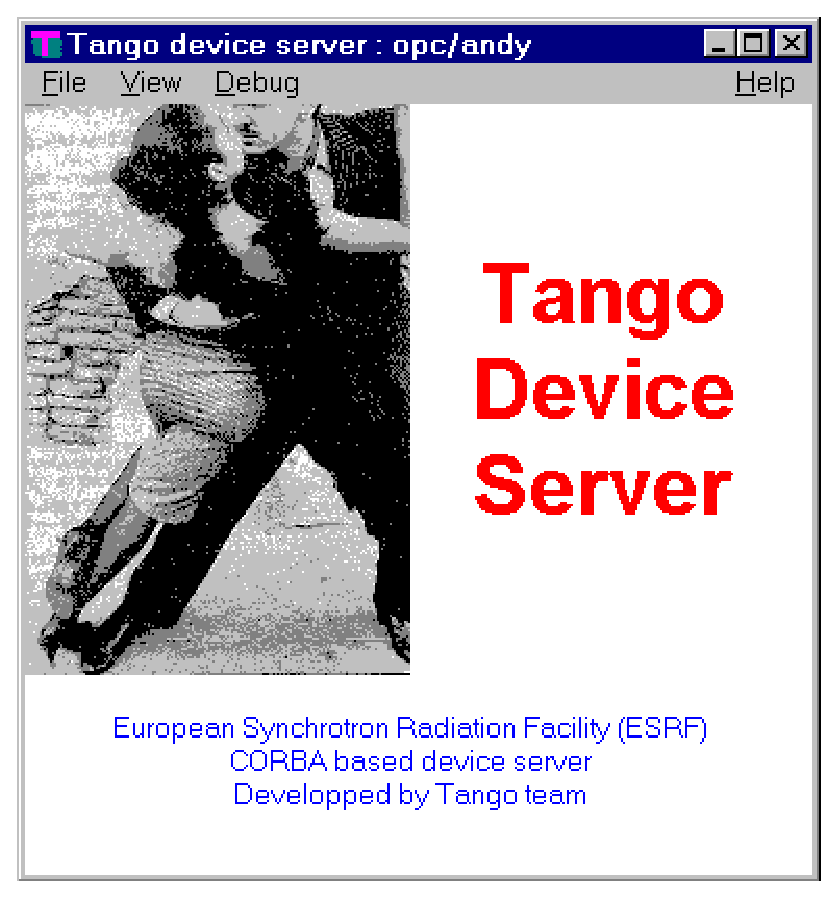
\includegraphics[width=10cm]{ds_writing/nt_server/main}
\end{figure}

\par\end{center}

\vspace{0.3cm}


Four menus are available in this window. The File menu allows the
user to exit the device server. The View menu allows you to display/hide
the device server console window. The Debug menu allows the user to
change the server output verbose\index{verbose} level. All the outputs
goes to the console window even if it is hidden. The Help menu displays
the help window. The device server name is displayed in the window
title. The text displayed at the bottom of the window has a default
value (the one displayed in this window dump) but may be changed by
the device server programmer using the \emph{set\_main\_window\_text(\index{set-main-window-text})}
method of the Tango::Util class. If used, this method must be called
prior to the call of the \emph{server\_init()\index{server-init}}
method. Refer to \cite{TANGO_ref_man} for a complete description
of this method.


\subsubsection{The console window}

This window looks like :

\vspace{0.3cm}


\begin{center}
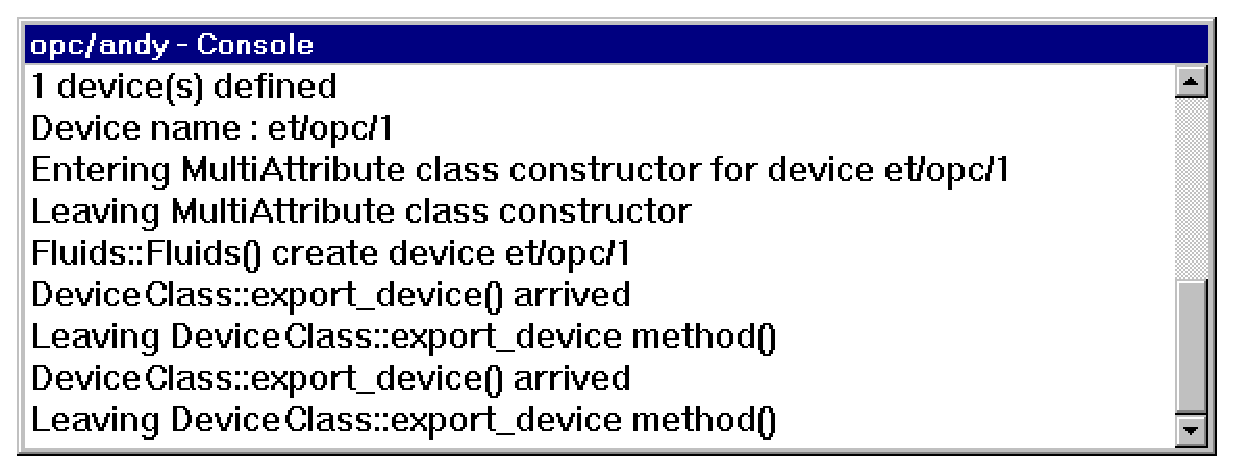
\includegraphics[width=14cm]{ds_writing/nt_server/cons}
\par\end{center}

\vspace{0.3cm}


It simply displays all the logging\emph{\index{logging}} message
when a console target is used in the device server. 


\subsubsection{The help window}

This window looks like :

\vspace{0.3cm}


\begin{center}
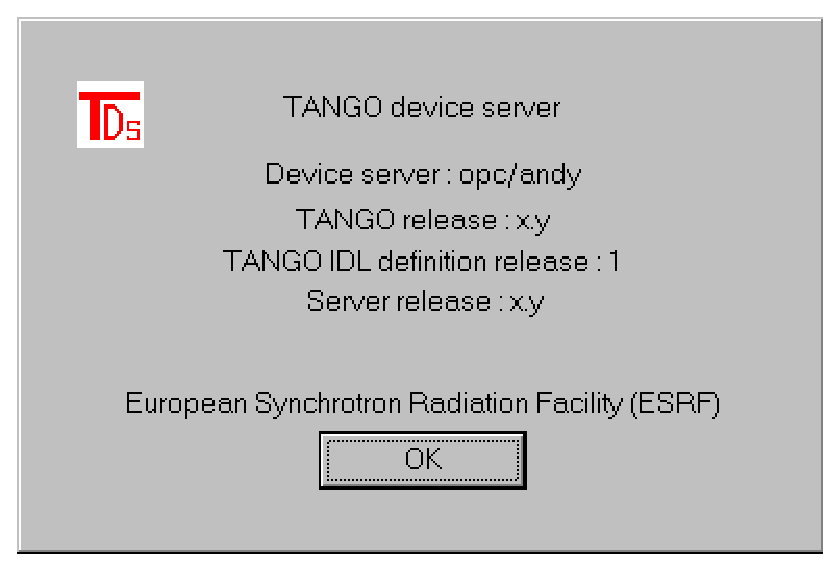
\includegraphics[width=9cm]{ds_writing/nt_server/help}
\par\end{center}



\vspace{0.3cm}


This window displays 
\begin{itemize}
\item The device server name
\item The Tango library release
\item The Tango IDL definition release
\item The device server release. The device server programmer may set this
release number using the \emph{set\_server\_version()\index{set-server-version}}
method of the Tango::Util\index{Util} class. If used, this must be
done prior to the call of the \emph{server\_init()} method. If the
\emph{set\_server\_version()} method is not used, x.y is displays
as version number. Refer to \cite{TANGO_ref_man} for a complete description
of this method.
\end{itemize}

\subsection{MFC device server}

There is no \emph{main} function within a classical MFC\index{MFC}
program. Most of the time, your application is represented by one
instance of a C++ class which inherits from the MFC CWinApp class.
This CWinApp class has several methods that you may overload in your
application class. For a device server to run correctly, you must
overload two methods of the CWinApp class. These methods are the \emph{InitInstance()\index{InitInstance}}
and \emph{ExitInstance()\index{ExitInstance}} methods. The rule of
these methods is obvious following their names.

\textbf{Remember that if the Tango device server graphical user interface
is used, you must link your device server with the Tango windows resource\index{resource}
file}. This is done by adding the Tango resource file to the Project
Settings/Link/Input/Object, library modules window in VC++.


\subsubsection{The InitInstance method}

The code to be added here is the equivalent of the code written in
a classical \emph{main()} function. Don't forget to add the \emph{tango.h}
file in the list of included files.


\begin{minted}[linenos]{cpp}
     1 BOOL FluidsApp::InitInstance()
     2 {
     3    AfxEnableControlContainer();
     4  
     5 // Standard initialization
     6 // If you are not using these features and wish to reduce the size
     7 //  of your final executable, you should remove from the following
     8 //  the specific initialization routines you do not need.
     9  
    10  #ifdef _AFXDLL
    11    Enable3dControls();          // Call this when using MFC in a shared DLL
    12  #else
    13    Enable3dControlsStatic();    // Call this when linking to MFC statically
    14  #endif
    15    Tango::Util *tg;
    16    try
    17    {
    18          
    19        tg = Tango::Util::init(m_hInstance,m_nCmdShow);
    20  
    21        tg->server_init(true);
    22  
    23        tg->server_run();
    24  
    25    }
    26    catch (bad_alloc)
    27    {
    28        MessageBox((HWND)NULL,"Memory error","Command line",MB_ICONSTOP);
    29        return(FALSE);
    30    }
    31    catch (Tango::DevFailed &e)
    32    {
    33        MessageBox((HWND)NULL,,e.errors[0].desc.in(),"Command line",MB_ICONSTOP);
    34        return(FALSE);
    35    }
    36    catch (CORBA::Exception &)
    37    {
    38        MessageBox((HWND)NULL,"Exception CORBA","Command line",MB_ICONSTOP);
    39        return(FALSE);
    40    }
    41  
    42    m_pMainWnd = new CWnd;
    43    m_pMainWnd->Attach(tg->get_ds_main_window());
    44  
    45    return TRUE;
    46  }
\end{minted}


Line 19 : Initialise Tango system. This method also analises the argument
used in command line.

Line 21 : Create Tango classes requesting the Tango Windows graphical\index{graphical}
interface to be used

Line 23 : Start Network listener. Note that under NT, this call returns
in the contrary of UNIX like operating system.

Line 26-30 : Display a message box in case of memory allocation error
and leave method with a return value set to false in order to stop
the process

Line 31-35 : Display a message box in case of error during server
initialization phase.

Line 36-40 : Display a message box in case of error other than memory
allocation. Leave method with a return value set to false in order
to stop the process.

Line 37-38 : Create a MFC\index{MFC} main window and attach the Tango
graphical interface main window to this MFC window.


\subsubsection{The ExitInstance\index{ExitInstance} method}

This method is called when the application is stopped. For Tango device
server, its rule is to destroy the Tango::Util singleton if this one
has been correctly constructed.


\begin{minted}[linenos]{cpp}
     1  int FluidsApp::ExitInstance()
     2  {
     3     bool del = true;
     4  
     5     try
     6     {
     7         Tango::Util *tg = Tango::Util::instance();
     8     }
     9     catch(Tango::DevFailed)
    10     {
    11         del = false;
    12     }
    13  
    14     if (del == true)
    15         delete (Tango::Util::instance());
    16  
    17     return CWinApp::ExitInstance();
    18  }
\end{minted}


Line 7 : Try to retrieve the Tango::Util singleton. If this one has
not been constructed correctly, this call will throw an exception.

Line 9-12 : Catch the exception in case of incomplete Tango::Util
singleton construction

Line 14-15 : Delete the Tango::Util singleton. This will unregister
the Tango device server from the Tango database.

Line 17 : Execute the \emph{ExitInstance} method of the CWinApp class.

If you don't want to use the Tango device server graphical interface,
do not pass any parameter to the \emph{server\_init()\index{server-init}}
method and instead of the code display in lines 37 and 38 in the previous
example of the \emph{InitInstance()} method, use your own code to
initialize your own application.


\subsubsection{Example of how to build a Windows device server MFC based}

This sub-chapter gives an example of what it is needed to do to build
a MFC Windows device server. Rather than being a list of actions to
strictly follow, this is some general rules of how using VC++ to build
a Tango device server using MFC.
\begin{enumerate}
\item Create your device server using Pogo. For a class named MyMotor, the
following files will be needed : \emph{class\_factory.cpp}, \emph{MyMotorClass.h},
\emph{MyMotorClass.cpp}, \emph{MyMotor.h} and \emph{MyMotor.cpp.}
\item On a Windows computer running VC++, create a new project of type ``MFC
app Wizard (exe)'' using static MFC\index{MFC} libs. Ask for a dialog
based project without ActiveX controls.
\item Copy the five files generated by Pogo to the Windows computer and
add them to your project
\item Remove the dialog window files (xxxDlg.cpp and xxxDlg.h), the Resource
include file and the resource script file from your project
\item Add \#include <stdafx.h> as first line of the include files list in
\emph{class\_factory.cpp}, \emph{MyMotorClass.cpp} and \emph{MyMotor.cpp}
file. Also add your own directory and the Tango include directory
to the project pre-compiler include directories list.
\item Enable RTTI in your project settings (see chapter \ref{Compiling NT})
\item Change your application class: 

\begin{enumerate}
\item Add the definition of an \emph{ExitInstance} method in the declaration
file. (xxx.h file)
\item Remove the include of the dialog window file in the xxx.cpp file and
add an include of the Tango master include files (tango.h)
\item Replace the \emph{InitInstance}() method as described in previous
sub-chapter. (xx.cpp file)
\item Add an \emph{ExitInstance()} method as described in previous sub-chapter
(xxx.cpp file)
\end{enumerate}
\item Add all the libraries needed to compile a Tango device server (see
chapter \ref{Compiling NT}) and the Tango resource file to the linker
Object/Libraries modules.
\end{enumerate}

\subsection{Win32 application}

Even if it is more natural to use the C++ structure of the MFC class
to write a Tango device server, it is possible to write a device server
as a Win32\index{Win32} application. Instead of having a \emph{main()}
function as the application entry point, the operating system, provides
a \emph{WinMain()} function as the application entry point. Some code
must be added to this \emph{WinMain\index{WinMain}} function in order
to support Tango device server. Don't forget to add the \emph{tango}.\emph{h}
file in the list of included files. If you are using the project files
generated by Pogo, don't forget to change the linker SUBSYSTEM option
to \textquotedbl{}Windows\textquotedbl{} (Under Linker/System in the
project properties window).


\begin{minted}[linenos]{cpp}
     1  int APIENTRY WinMain(HINSTANCE hInstance,
     2                       HINSTANCE hPrevInstance,
     3                       LPSTR     lpCmdLine,
     4                       int       nCmdShow)
     5  {
     6     MSG msg;
     7     Tango::Util *tg;
     8  
     9     try
    10     {
    11         tg = Tango::Util::init(hInstance,nCmdShow);
    12  
    13         string txt;
    14         txt = "Blabla first line\n";
    15         txt = txt + "Blabla second line\n";
    16         txt = txt + "Blabla third line\n";
    17         tg->set_main_window_text(txt);
    18         tg->set_server_version("2.2");
    19  
    20         tg->server_init(true);
    21  
    22         tg->server_run();
    23  
    24     }
    25     catch (bad_alloc)
    26     {
    27         MessageBox((HWND)NULL,"Memory error","Command line",MB_ICONSTOP);
    28         return (FALSE);
    29     }
    30     catch (Tango::DevFailed &e)
    31     {
    32         MessageBox((HWND)NULL,e.errors[0].desc.in(),"Command line",MB_ICONSTOP);
    33         return (FALSE);
    34     }
    35     catch (CORBA::Exception &)
    36     {
    37         MessageBox((HWND)NULL,"Exception CORBA","Command line",MB_ICONSTOP);
    38         return(FALSE);
    39     }
    40  
    41     while (GetMessage(&msg, NULL, 0, 0)) 
    42     {
    43         TranslateMessage(&msg);
    44         DispatchMessage(&msg);
    45     }
    46  
    47     delete tg;
    48  
    49     return msg.wParam;
    50  }
\end{minted}


Line 11 : Create the Tango::Util\index{Util} singleton

Line 13-18 : Set parameters for the graphical interface

Line 20 : Initialize Tango device server requesting the display of
the graphical interface

Line 22 : Run the device server

Line 25-39 : Display a message box for all the kinds of error during
Tango device server initialization phase and exit WinMain\index{WinMain}
function.

Line 41-45 : The Windows message loop

Line 47 : Delete the Tango::Util singleton. This class destructor
unregisters the device server from the Tango database.

\textbf{Remember that if the Tango device server graphical user interface
is used, you must add the Tango windows resource\index{resource}
file} \textbf{to your project}.

If you don't want to use the tango device server graphical user interface,
do not use any parameter in the call of the \emph{server\_init()\index{server-init}}
method and do not link your device server with the Tango Windows resource
file.


\subsection{Device server as service}

With Windows, if you want to have processes which survive to logoff
sequence and/or are automatically started during computer startup
sequence, you have to write them as service\index{service}. It is
possible to write Tango device server as service. You need to
\begin{enumerate}
\item Write a class which inherits from a pre-written Tango class called
NTService. This class must have a \emph{start\index{start}} method. 
\item Write a main function following a predefined skeleton.
\end{enumerate}

\subsubsection{The service class}

It must inherits from the \emph{NTService} class and defines a \emph{start}
method. The NTService\index{NTService} class must be constructed
with one argument which is the device server executable\index{executable}
name. The \emph{start} method has three arguments which are the number
of arguments passed to the method, the argument list and a reference
to an object used to log info in the NT event system. The first two
args must be passed to the Tango::Util::init method and the last one
is used to log error or info messages. The class definition file looks
like


\begin{minted}[linenos]{cpp}
     1  #include <tango.h>
     2  #include <ntservice.h>
     3  
     4  class MYService: public Tango::NTService
     5  {
     6  public:
     7     MYService(char *);
     8  
     9     void start(int,char **,Tango::NTEventLogger *);
    10  };
\end{minted}




Line 1-2 : Some include files

Line 4 : The MYService class inherits from \emph{Tango::NTService}
class

Line 7 : Constructor with one parameter

Line 9 : The \emph{start()\index{start}} method\\


The class source code looks like


\begin{minted}[linenos]{cpp}
     1  #include <myservice.h>
     2  #include <tango.h>
     3  
     4  using namespace std;
     5  
     6  MYService::MYService(char *exec_name):NTService(exec_name)
     7  {
     8  }
     9  
    10  void MYService::start(int argc,char **argv,Tango::NTEventLogger *logger)
    11  {
    12     Tango::Util *tg;
    13     try
    14     {
    15        Tango::Util::_service = true;
    16  
    17        tg = Tango::Util::init(argc,argv);
    18  
    19        tg->server_init();
    20  
    21        tg->server_run();
    22     }
    23     catch (bad_alloc)
    24     {
    25        logger->error("Can't allocate memory to store device object");
    26     }
    27     catch (Tango::DevFailed &e)
    28     {
    29        logger->error(e.errors[0].desc.in());
    30     }
    31     catch (CORBA::Exception &)
    32     {
    33        logger->error("CORBA Exception");
    34     }
    35  }
\end{minted}




Line 6-8 : The MYService class constructor code.

Line 15 : Set to true the \emph{\_service} static variable of the
\emph{Tango::Util} class.

Line 17-21 : Classical Tango device server startup code

Line 23-34 : Exception management. Please, note that within a service.
it is not possible to print data on a console. This method receives
a reference to a logger\index{logger} object. This object sends all
its output to the Windows event\index{event} system. It is used to
send messages when an exception has occurred.


\subsubsection{The main function}

The main function is used to create one instance of the class describing
the service, to check the service option and to run the service. The
code looks like :


\begin{minted}[linenos]{cpp}
     1  #include <tango.h>
     2  #include <MYService.h>
     3  
     4  using namespace std;
     5  
     6  
     7  int main(int argc,char *argv[])
     8  {
     9     MYService service(argv[0]);
    10          
    11     int ret;
    12     if ((ret = service.options(argc,argv)) <= 0)
    13         return ret;
    14          
    15     service.run(argc,argv);
    16          
    17     return 0;
    18  }
\end{minted}


Line 9 : Create one instance of the MYService class with the executable
name as parameter

Line 12 : Check service option with the \emph{options()} method inherited
from the NTService\index{NTService} class.

Line 15 : Run the service. The \emph{run()} method is inherited from
the NTService class. This method will after some NT initialization
sequence execute the user \emph{start()\index{start}} method.


\subsubsection{Service options and messages}

When a Tango device server is written as a Windows service, it supports
several new options. These option are linked to Windows service\index{service}
usage.

Before it can be used, a service must be installed. A name and a title
is associated to each service. For Tango device server used as service,
the service name is build from the executable name followed by the
underscore character and the instance name. For example, a device
server service executable file named ``opc'' and started with ``fluids''
as instance name, will be named ``opc\_fluids''. The title string
is built from the service executable name followed by the sentence
``Tango device server'' and the instance name between parenthesis.
In the previous example, the service title will be ``opc Tango device
server (fluids)''. Once a service is installed, you can configure
it with the ``Services'' application of the control panel. Services
title are displayed by this application and allow the user to select
one specific service. Once a service is selected, it is possible to
start/stop it and to configure its startup type as manual (with the
Services application) or as automatic. When the automatic mode is
chosen, the service starts when the computer is started. In this case,
the service executable code must resides on the computer local disk.

Tango device server logs message in the Windows event\index{event}
system when the service is started or stopped. You can see these messages
with the ``Event Viewer'' application (Start->Programs->Administrative
tools->Event Viewer) and choose the Application events.

The new options are -i, -s, -u, -h and -d.
\begin{itemize}
\item -i : Install the service\index{service}
\item -s : Install the service and choose the automatic startup mode
\item -u : Un-install the service
\item -dbg : Run in console mode to debug service. The service must have
been installed prior to used it. The classical -v device server option
can be used with the -d option.
\end{itemize}
On the command line, all these options must be used after the device
server instance name (``opc fluids -i'' to install the service,
``opc fluids -u'' to un-install the service, ``opc fluids -v -d''
to debug the service)


\subsubsection{Tango device server using MFC as Windows service}

If your Tango device server uses MFC\index{MFC} and must be written
as a Windows NT service, follow these rules :
\begin{itemize}
\item Don't forget to add the \emph{stdafx.h} file as the first file included
in all the source files making the project.
\item Comment out the definition of VC\_EXTRALEAN in the \emph{stdafx.h}
file.
\item Change the pre-processor definitions, replace \_WINDOWS by \_CONSOLE
\item Add the /SUBSYSTEM:CONSOLE option in the linker options window of
the project settings.
\item Add a call to initialize the MFC (\emph{AfxWinInit()}) in the service
main function
\end{itemize}

\begin{minted}[linenos]{cpp}
     1  int main(int argc,char *argv[])
     2  {
     3     if (!AfxWinInit(::GetModuleHandle(NULL),NULL,::GetCommandLine(),0))
     4     {
     5        cerr << "Can't initialise MFC !" << endl;
     6        return -1;
     7     }
     8  
     9     service serv(argv[0]);
    10  
    11     int ret;
    12     if ((ret = serv.options(argc,argv)) <= 0)
    13          return ret;
    14  
    15     serv.run(argc,argv);
    16  
    17     return 0;
    18  }
\end{minted}


Line 3 : The MFC classes are initialized with the \emph{AfxWinInit()}
function call.


\section{Compiling, linking and executing a TANGO device server process}
\label{sec:Compiling,-linking-and}


\subsection{Compiling and linking a C++ device server}


\subsubsection{On UNIX like operating system }


\paragraph{Supported development tools}

The supported compiler for Linux is \textbf{gcc\index{gcc}} release
3.3 and above. Please, note that to debug a Tango device server running
under Linux\index{Linux}, \textbf{gdb\index{gdb}} release 7 and
above is needed in order to correctly handle threads.


\paragraph{Compiling\index{compiling}}

TANGO for C++ uses omniORB (release 4) as underlying CORBA Object
Request Broker \cite{OOC page} and starting with Tango 8, the ZMQ
library. To compile a TANGO device server, your include search path
must be set to :
\begin{itemize}
\item The omniORB include directory
\item The ZMQ\index{ZMQ} include directory
\item The Tango include directory
\item Your development directory
\end{itemize}

\paragraph{Linking\index{linking} }

To build a running device server process, you need to link your code
with several libraries. Nine of them are always the same whatever
the operating system used is. These nine libraries are:
\begin{itemize}
\item The Tango libraries (called \textbf{libtango} and \textbf{liblog4tango})
\item Three omniORB\index{omniORB} package libraries (called \textbf{libomniORB4},
\textbf{libomniDynamic4} and \textbf{libCOS4)}
\item The omniORB threading library (called \textbf{libomnithread})
\item The ZMQ library (callled \textbf{libzmq})
\end{itemize}
On top of that, you need additional libraries depending on the operating
system :
\begin{itemize}
\item For Linux, add the posix thread library (\textbf{libpthread})
\end{itemize}
The following table summarizes the necessary options to compile a
Tango C++ device server. Please, note that starting with Tango 8 and
for gcc release 4.3 and later, some C++11\index{C++11} code has been
used. This requires the compiler option \textquotedbl{}-std=c++0x\textquotedbl{}.
Obviously, the options -I and -L must be updated to reflect your file
system organization. 

\vspace{0.3cm}


\begin{center}
\begin{longtable}{|c|c|m{70mm}|}
\hline 
Operating system & Compiling option & Linking option\tabularnewline
\hline 
\hline 
Linux gcc & -D\_REENTRANT -std=c++0x -I.. & -L.. -ltango -llog4tango -lomniORB4 -lomniDynamic4 -lCOS4 -lomnithread
-lzmq -lpthread\tabularnewline
\hline 
\end{longtable}
\par\end{center}

\vspace{0.3cm}


The following is an example of a Makefile for Linux. Obviously, all
the paths are set to the ESRF file system structure.


\begin{minted}[linenos]{cpp}
1 #
2 # Makefile to generate a Tango server
3 #
4 
5 CC = c++
6 BIN_DIR = ubuntu1104
7 TANGO_HOME = /segfs/tango
8 
9 INCLUDE_DIRS = -I $(TANGO_HOME)/include/$(BIN_DIR) -I .
10
11 
12 LIB_DIRS = -L $(TANGO_HOME)/lib/$(BIN_DIR)
13 
14 
15 CXXFLAGS = -D_REENTRANT -std=c++0x $(INCLUDE_DIRS)
16 LFLAGS = $(LIB_DIRS) -ltango \
17                      -llog4tango \
18                      -lomniORB4 \
19                      -lomniDynamic4 \
20                      -lCOS4 \
21                      -lomnithread \
22                      -lzmq \
23                      -lpthread
24 
25 
26 SVC_OBJS = main.o \
27            ClassFactory.o \
28            SteppermotorClass.o \
29            Steppermotor.o \
30            SteppermotorStateMachine.o
31 
32 
33 .SUFFIXES: .o .cpp
34 .cpp.o:
35     $(CC) $(CXXFLAGS) -c $<
36 
37 
38 all: StepperMotor
39 
40 StepperMotor: $(SVC_OBJS)
41     $(CC) $(SVC_OBJS) -o $(BIN_DIR)/StepperMotor $(LFLAGS)
42 
43 clean:
44     rm -f *.o core
\end{minted}




Line 5-7 : Define Makefile macros

Line 9-10 : Set the include file search path

Line 12 : Set the linker library search path

Line 15 : The compiler option setting

Line 16-23 : The linker option setting

Line 26-30 : All the object files needed to build the executable

Line 33-35 : Define rules to generate object files

Line 38 : Define a ``all'' dependency

Line 40-41 : How to generate the StepperMotor device server executable

Line 43-44 : Define a ``clean'' dependency


\subsubsection{On Windows using Visual Studio}
\label{Compiling NT}

Supported Windows\index{Windows} compiler for Tango is Visual Studio
2008 (VC 9), Visual Studio 2010 (VC10) and Visual Studio 2013 (VC12).
Most problems in building a Windows device server revolve around the
/M compiler switch family. This switch family controls which run-time
library names are embedded in the object files, and consequently which
libraries are used during linking\index{linking}. Attempt to mix
and match compiler settings and libraries can cause link error and
even if successful, may produce undefined run-time behavior.

Selecting the correct /M switch in Visual Studio is done through a
dialog box. To open this dialog box, click on the ``Project'' menu
(once the correct project is selected in the Solution Explorer window)
and select the ``Properties'' option. To change the compiler switch
open the ``C/C++'' tree and select ``Code Generation''. The following
options are supported.
\begin{itemize}
\item Multithreaded = /MT
\item Multithreaded DLL = /MD
\item Debug Multithreaded = /MTd
\item Debug Multithreaded DLL = /MDd
\end{itemize}
Compiling a file with a value of the /M switch family will impose
at link phase the use of libraries also compiled with the same value
of the /M switch family. If you compiled your source code with the
/MT option (Multithreaded), you must link it with libraries also compiled
with the /MT option.

On both 32 or 64 bits computer, omniORB and TANGO relies on the preprocessor
identifier \textbf{WIN32}\index{WIN32} being defined in order to
configure itself. If you build an application using static libraries
(option /MT or /MTd), you must add \textbf{\_WINSTATIC} to the list
of the preprocessor identifiers. If you build an application using
DLL\index{DLL} (option /MD or /MDd), you must add \textbf{LOG4TANGO\_HAS\_DLL}
and \textbf{TANGO\_HAS\_DLL} to the list of preprocessor identifiers.

To build a running device server process, you need to link your code
with several libraries on top of the Windows libraries. These libraries
are:
\begin{itemize}
\item The Tango libraries (called \textbf{tango.lib} and \textbf{log4tango.lib}
or \textbf{tangod.lib} and \textbf{log4tangod.lib} for debug mode)
\item The omniORB\index{omniORB} package libraries (see next table)\\

\end{itemize}
\begin{center}
\begin{longtable}{|c|c|}
\hline 
Compile mode & Libraries\tabularnewline
\hline 
\hline 
Debug Multithreaded & omniORB4d.lib, omniDynamic4d.lib, omnithreadd.lib and COS4d.lib\tabularnewline
\hline 
Multithreaded & omniORB4.lib, omniDynamic4.lib, omnithread.lib and COS4.lib\tabularnewline
\hline 
Debug Multithreaded DLL & omniORB420\_rtd.lib, omniDynamic420\_rtd.lib, omnithread40\_rtd.lib,\tabularnewline
 & and COS420\_rtd.lib\tabularnewline
\hline 
Multithreaded DLL & omniORB420\_rt.lib, omniDynamic420\_rt.lib, omnithread40\_rt.lib\tabularnewline
 & and COS420\_rt.lib\tabularnewline
\hline 
\end{longtable}
\par\end{center}
\begin{itemize}
\item The ZMQ library (\textbf{zmq.lib} or \textbf{zmqd.lib} for debug mode)
\item Windows network libraries (\textbf{mswsock.lib} and \textbf{ws2\_32.lib})
\item Windows graphic library (\textbf{comctl32.lib})
\end{itemize}
To add these libraries in Visual Studio, open the project property
pages dialog box and open the ``Link'' tree. Select ``Input''
and add these library names to the list of library in the ``Additional
Dependencies'' box. 

The ``Win32 Debug'' or ``Win32 Release'' configuration that you
change within the \textquotedbl{}Configuration Manager\textquotedbl{}
window changes the /M switch compiler. For instance, if you select
a ``Win32 Debug'' configuration in a \textquotedbl{}non-DLL\textquotedbl{}
project, use the omniORB4d.lib, omniDynamic4d.lib and omnithreadd.lib
libraries plus the tangod.lib, log4tangod.lib and zmqd.lib libraries.
If you select the ``Win32 Release'' configuration, use the omniORB4.lib,
omniDynamic4.lib and omnithread.lib libraries plus the tango.lib,
log4tango.lib and zmq.lib libraries.

\textbf{WARNING}: In some cases, the Microsoft Visual Studio wizard
used during project creation generates one include file called \emph{Stdafx.h}.
If this file itself includes windows.h file, you have to add the preprocessor
macro \_WIN32\_WINNT\index{-WIN32-WINNT} and set it to 0x0500.


\subsection{Running a C++ device server}
\label{Env variable}

To run a C++ Tango device server, you must set an environment variable.
This environment variable is called \textbf{TANGO\_HOST\index{TANGO-HOST}}
and has a fixed syntax which is \begin{center}TANGO\_HOST=<host>:<port>\end{center}The
host field is the host name where the TANGO database device server
is running. The port field is the port number on which this server
is listening. For instance, a valid syntax is TANGO\_HOST=dumela:10000.
For UNIX like operating system, setting environment variable is possible
with the \emph{export} or \emph{setenv} command depending on the shell
used. For Windows, setting environment variable is possible with the
``Environment'' tab of the ``System'' application in the control
panel.

If you need to start a Tango device server on a pre-defined port\index{port}
(For Tango database device server or device server without database
usage), you must use one of the underlying ORB option \emph{endPoint}
like \begin{center}myserver myinstance\_name -ORBendPoint giop:tcp::<port
number>\end{center}


\section{Advanced programming techniques}

The basic techniques for implementing device server pattern are required
by each device server programmer. In certain situations, it is however
necessary to do things out of the ordinary. This chapter will look
into programming techniques which permit the device server serve more
than simply the network.


\subsection{Receiving signal}

It is \textbf{UNSAFE} to use any CORBA call in a signal handler. It
is also UNSAFE to use some system calls in a signal handler. Tango
device server solved this problem by using threads\index{thread}.
A specific thread is started to handle signals\index{signal}. Therefore,
every Tango device server is automatically a threaded process. This
allows the programmer to write the code which must be executed when
a signal is received as ordinary code. All device server threads masks
all signals except the specific signal thread which is permanently
waiting for signal. If a signal is sent to a device server process,
only the signal thread will receive it because it is the single thread
which does not mask signals.

Nevertheless, signal management is not trivial and some care have
to be taken. The signal management differs from operating system to
operating system. It is not recommended that you install your own
signal routine using any of the signal routines provided by the operating
system calls or library. 


\subsubsection{Using signal}

It is possible for C++ device server to receive signals from drivers
or other processes. The TDSOM supports receiving signal at two levels:
the device level and the class level. Supporting signal at the device
level means that it is possible to specify interest into receiving
signal on a device basis. This feature is supported via three methods
defined in the DeviceImpl\index{DeviceImpl} class. These methods
are called \emph{register\_signal}, \emph{unregister\_signal} and
s\emph{ignal\_handler}.

The \textbf{\emph{register\_signal\index{register-signal}}} method
has one parameter which is the signal number. This method informs
the device server signal system that the device want to be informed
when the signal passed as parameter is received by the process. There
is a special case for Linux as explained in the previous sub-chapter.
It is possible to register a signal to be executed in the a signal
handler context (with all its restrictions). This is done with a second
parameter to this \emph{register\_signal} method. This second parameter
is simply a boolean data. If it is true, the signal\_handler will
be executed in a signal handler context in the device server main
thread. A default value (false) has been defined for this parameter.

The \textbf{\emph{unregister\_signal\index{unregister-signal}}} method
also have an input parameter which is the signal number. This method
removes the device from the list of object which should be warned
when the signal is received by the process.

The \textbf{\emph{signal\_handler\index{signal-handler}}} method
is the method which is triggered when a signal is received if the
corresponding \emph{register\_signal} has been executed. This method
is defined as virtual and can be redefined by the user. It has one
input argument which is the signal number.

The same three methods also exist in the DeviceClass\index{DeviceClass}
class. Their action and their usage are similar to the DeviceImpl
class methods. Installing a signal at the class level does not mean
that all the device belonging to this class will receive the signal.
This only means that the \emph{signal\_handler} method of the DeviceClass
instance will be executed. This is useful if an action has to be executed
once for a class of devices when a signal is received.

The following code is an example with our stepper motor device server
configured via the database to serve three motors. These motors have
the following names : id04/motor/01, id04/motor/02 and id04/motor/03.
The signal SIGALRM (alarm signal) must be propagated only to the motor
number 2 (id04/motor/02)


\begin{minted}[linenos]{cpp}
 1  void StepperMotor::init_device()
 2  {
 3      cout << "StepperMotor::StepperMotor() create motor " << dev_name << endl;
 4  
 5      long i;
 6  
 7      for (i=0; i< AGSM_MAX_MOTORS; i++)
 8      {
 9          axis[i] = 0;
10          position[i] = 0;
11          direction[i] = 0;
12      }
13  
14      if (dev_name == "id04/motor/02")
15          register_signal(SIGALRM);
16  }
17  
18  StepperMotor::~StepperMotor()
19  {
20      unregister_signal(SIGALRM);
21  }
22  
23  void StepperMotor::signal_handler(long signo)
24  {
25      INFO_STREAM << "Inside signal handler for signal " << signo << endl;
26  
27  //  Do what you want here
28  
29  }
\end{minted}


The \emph{init\_device} method is modified.

Line 14-15 : The device name is checked and if it is the correct name,
the device is registered in the list of device wanted to receive the
SIGALARM signal.

The destructor is also modified

Line 20 : Unregister the device from the list of devices which should
receives the SIGALRM signal. Note that unregister a signal for a device
which has not previously registered its interest for this signal does
nothing.

The \emph{signal\_handler} method is redefined

Line 25 : Print signal number

Line 27 : Do what you have to do when the signal SIGALRM is received.

If all devices must be warned when the device server process receives
the signal SIGALRM, removes line 14 in the \emph{init\_device} method.


\subsubsection{Exiting a device server gracefully}

A device server\index{server} has to exit\index{exit} gracefully
by unregistering itself from the database. The necessary action to
gracefully exit are automatically executed on reception of the following
signal\index{signal} :
\begin{itemize}
\item SIGINT, SIGTERM and SIGQUIT for device server running on Linux
\item SIGINT, SIGTERM, SIGABRT and SIGBREAK for device server running on
Windows
\end{itemize}
This does not prevents device server to also register interest at
device or class levels for those signals. The user installed \emph{signal\_handler\index{signal-handler}}
method will first be called before the graceful exit.


\subsection{Inheriting}
\label{Inheriting}

This sub-chapter details how it is possible to inherit\index{inherit}
from an existing device pattern implementation. As the device pattern
includes more than a single class, inheriting from an existing device
pattern needs some explanations.

Let us suppose that the existing device pattern implementation is
for devices of class A. This means that classes A and AClass already
exists plus classes for all commands offered by device of class A.
One new device pattern\index{pattern} implementation for device of
class B must be written with all the features offered by class A plus
some new one. This is easily done with the inheritance. Writing a
device pattern implementation for device of class B which inherits
from device of class A means :
\begin{itemize}
\item Write the BClass class
\item Write the B class
\item Write B class specific commands
\item Eventually redefine A class commands
\end{itemize}
The miscellaneous code fragments given below detail only what has
to be updated to support device pattern inheritance


\subsubsection{Writing the BClass}

As you can guess, BClass has to inherit from AClass. The \emph{command\_factory\index{command-factory}}
method must also be adapted.


\begin{minted}[linenos]{cpp}
     1  namespace B
     2  {
     3  
     4  class BClass : public A::AClass
     5  {
     6  .....
     7  }
     8  
     9  BClass::command_factory()
    10  {
    11      A::AClass::command_factory();
    12  
    13      command_list.push_back(....);
    14  }
    15  
    16  } /* End of B namespace */
\end{minted}


Line 1 : Open the B namespace

Line 4 : BClass inherits from AClass which is defined in the A namespace.

Line 11 : Only the \emph{command\_factory} method of the BClass will
be called at start-up. To create the AClass commands, the \emph{command\_factory}
method of the AClass must also be executed. This is the reason of
the line

Line 13 : Create BClass commands


\subsubsection{Writing the B class}

As you can guess, B has to inherits\index{inherit} from A.


\begin{minted}[linenos]{cpp}
     1  namespace B
     2  {
     3  
     4  class B : public A:A
     5  {
     6     .....
     7  };
     8  
     9  B::B(Tango::DeviceClass *cl,const char *s):A::A(cl,s)
    10  {
    11     ....
    12     init_device();
    13  }
    14  
    15  void B::init_device()
    16  {
    17     ....
    18  }
    19  
    20  } /* End of B namespace */
\end{minted}


Line 1 : Open the B namespace.

Line 4 : B inherits from A which is defined in the A namespace

Line 9 : The B constructor calls the right A constructor


\subsubsection{Writing B class specific command}

Noting special here. Write these classes as usual


\subsubsection{Redefining A class command\index{command}}

It is possible to redefine a command which already exist in class
A \textbf{only if the command is created} \textbf{using the inheritance\index{inheritance}
model} (but keeping its input and output argument types). The method
which really execute the class A command is a method implemented in
the A class. This method must be defined as \textbf{virtual.} In class
B, you can redefine the method executing the command and implement
it following the needs of the B class.




\subsection{Using another device pattern implementation within the same server}

It is often necessary that inside the same device server\index{server},
a method executing a command needs a command of another class to be
executed. For instance, a device pattern implementation for a device
driven by a serial line class can use the command offered by a serial
line class embedded within the same device server process. To execute
one of the command (or any other CORBA\index{CORBA} operations/attributes)
of the serial line class, just call it as a normal client will do
by using one instance of the DeviceProxy class\emph{.} The ORB will
recognize that all the devices are inside the same process and will
execute calls as a local\index{local} calls. To create the DeviceProxy
class instance, the only thing you need to know is the name of the
device you gave to the serial line device. Retrieving this could be
easily done by a Tango device property. The DeviceProxy class is fully
described in Tango Application Programming Interface (API) reference
WEB pages


\subsection{Device pipe\index{pipe}}

What a Tango device pipe is has been defined in the Chapter 3 about
device server model. How you read or write a pipe in a client software
is documented in chapter 4 about the Tango API. In this section, we
describe how you can read/write into/from a device pipe on the server
side (In a Tango class with pipe).


\subsubsection{Client reading a pipe}

When a client reads a pipe, the following methods are executed in
the Tango class:
\begin{enumerate}
\item The \emph{always\_executed\_hook()} method.
\item A method called \emph{is\_<pipe\_name>\_allowed()}. The rule of this
method is to allow (or disallow) the next method to be executed. It
is usefull for device with some pipes which can be read only in some
precise conditions. It has one parameter which is the request type
(read or write)
\item A method called \emph{read\_<pipe\_name>()}. The aim of this method
is to store the pipe data in the pipe object. It has one parameter
which is a reference to the Pipe object to be read.
\end{enumerate}
The figure \ref{r_pipe_timing_fig-1} is a drawing of these method
calls sequencing for our class StepperMotor with one pipe named DynData.
\begin{figure}[H]
\begin{centering}
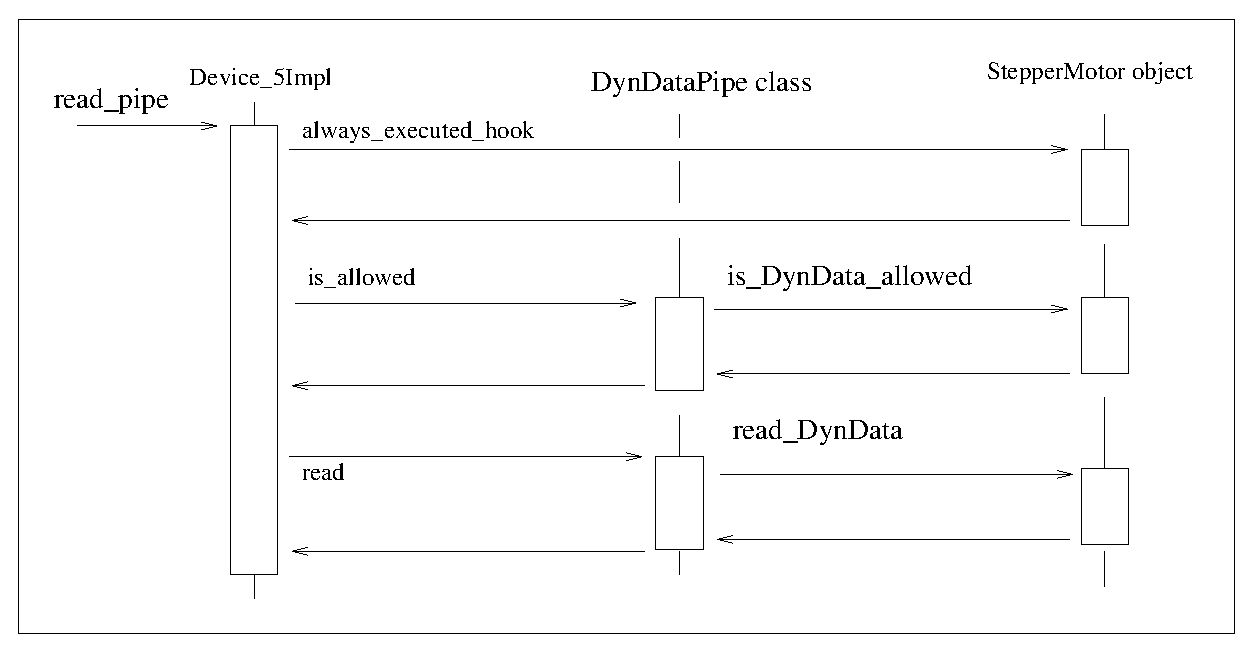
\includegraphics[scale=0.7]{ds_writing/r_pipe}
\par\end{centering}

\protect\caption{Read pipe sequencing}
\label{r_pipe_timing_fig-1}
\end{figure}


The class DynDataPipe is a simple class which follow the same skeleton
from one Tango class to another. Therefore, this class is generated
by the Tango code generator Pogo and the Tango class developper does
not have to modify it. The method \emph{is\_DynData\_allowed()} is
relatively simple and in most cases the default code generated by
Pogo is enough. The method \emph{read\_DynData()} is the method on
which the Tango class developper has to concentrate on. The following
code is one example of these two methods.


\begin{minted}[linenos]{cpp}
     1  bool StepperMotor::is_DynData_allowed(Tango::PipeReqType req)
     2  {
     3      if (get_state() == Tango::ON)
     4          return true;
     5      else
     6          return false;
     7  }
     8
     9  void StepperMotor::read_DynData(Tango::Pipe &pipe)
    10  {
    11      nb_call++;
    12      if (nb_call % 2 == 0)
    13      {
    14          pipe.set_root_blob_name("BlobCaseEven");
    15
    16          vector<string> de_names {"EvenFirstDE","EvenSecondDE"};
    17          pipe.set_data_elt_names(de_names);
    18
    19          dl = 666;
    20          v_db.clear();
    21          v_db.push_back(1.11);
    22          v_db.push_back(2.22);
    23
    24          pipe << dl << v_db;
    25      }
    26      else
    27      {
    28          pipe.set_root_blob_name("BlobCaseOdd");
    29
    30          vector<string> de_names {"OddFirstDE"};
    31          pipe.set_data_elt_names(de_names);
    32
    33          v_str.clear();
    34          v_str.push_back("Hola");
    35          v_str.push_back("Salut");
    36          v_str.push_back("Hi");
    37
    38          pipe << v_str;
    39      }
    40  }
\end{minted}


The \emph{is\_DynData\_allowed} method is defined between lines 1
and 7. It is allowed to read or write the pipe only is the device
state is ON. Note that the input parameter req is not used. The parameter
allows the user to know the type of request. The data type PipeReqType
is one enumeration with two possible values which are READ\_REQ and
WRITE\_REQ.

The \emph{read\_DynData} method is defined between lines 9 and 40.
If the number of times this method has been called is even, the pipe
contains two data elements. The first one is named EvenFirstDE and
its data is a long. The second one is named EvenSecondDE and its data
is an array of double. If the number of call is odd, the pipe contains
only one data element. Its name is OddFirstDe and its data is an array
of strings. Data are inserted into the pipe at lines 24 and 38. The
variables nb\_call, dl, v\_db and v\_str are device data member and
therefore declare in the .h file. Refer to pipe section in chapter
3 and to the API reference documentation (in Tango WEB pages) to learn
more on how you can insert data into a pipe and to know how data are
organized within a pipe.


\subsubsection{Client writing a pipe}

When a client writes a pipe, the following methods are executed in
the Tango class:
\begin{enumerate}
\item The \emph{always\_executed\_hook()} method.
\item A method called \emph{is\_<pipe\_name>\_allowed()}. The rule of this
method is to allow (or disallow) the next method to be executed. It
is usefull for device with some pipes which can be read only in some
precise conditions. It has one parameter which is the request type
(read or write)
\item A method called \emph{write\_<pipe\_name>()}. It has one parameter
which is a reference to the WPipe object to be written. The aim of
this method is to get the data to be written from the WPipe oject
and to write them into the corresponding Tango class objects.
\end{enumerate}
The figure \ref{w_pipe_timing_fig-1-1} is a drawing of these method
calls sequencing for our class StepperMotor with one pipe named DynData.
\begin{figure}[H]
\begin{centering}
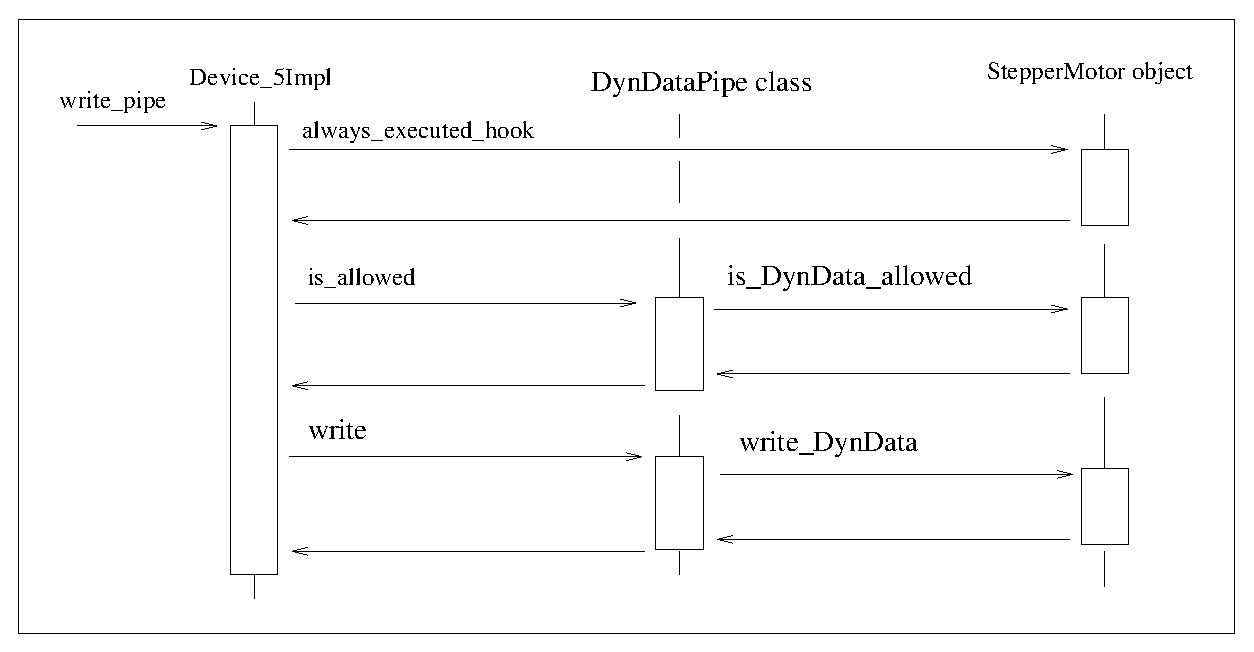
\includegraphics[scale=0.7]{ds_writing/w_pipe}
\par\end{centering}

\protect\caption{Write pipe sequencing}
\label{w_pipe_timing_fig-1-1}
\end{figure}


The class DynDataPipe is a simple class which follow the same skeleton
from one Tango class to another. Therefore, this class is generated
by the Tango code generator Pogo and the Tango class developper does
not have to modify it. The method \emph{is\_DynData\_allowed()} is
relatively simple and in most cases the default code generated by
Pogo is enough. The method \emph{write\_DynData()} is the method on
which the Tango class developper has to concentrate on. The following
code is one example of the \emph{write\_DynData()} method.


\begin{minted}[linenos]{cpp}
     1  void StepperMotor::write_DynData(Tango::WPipe &w_pipe)
     2  {
     3     string str;
     4     vector<float> v_fl;
     5
     6     w_pipe >> str >> v_fl;
     7     .....
     8  }
\end{minted}


In this example, we know that the pipe will always contain a srting
followed by one array of float. On top of that, we are not niterested
by the

data element names. Data are extracted from the pipe at line 6 and
are available for further use starting at line 7. If the content of
the pipe is not a string followed by one array of float, the data
extraction line (6) will throw one exception which will be reported
to the client who has tried to write the pipe. Refer to pipe section
in chapter 3 and to the API reference documentation (in Tango WEB
pages) to learn more on how you can insert data into a pipe and to
know how data are organized within a pipe.

\bigskip{}


\begin{center}

\label{BlackPicture}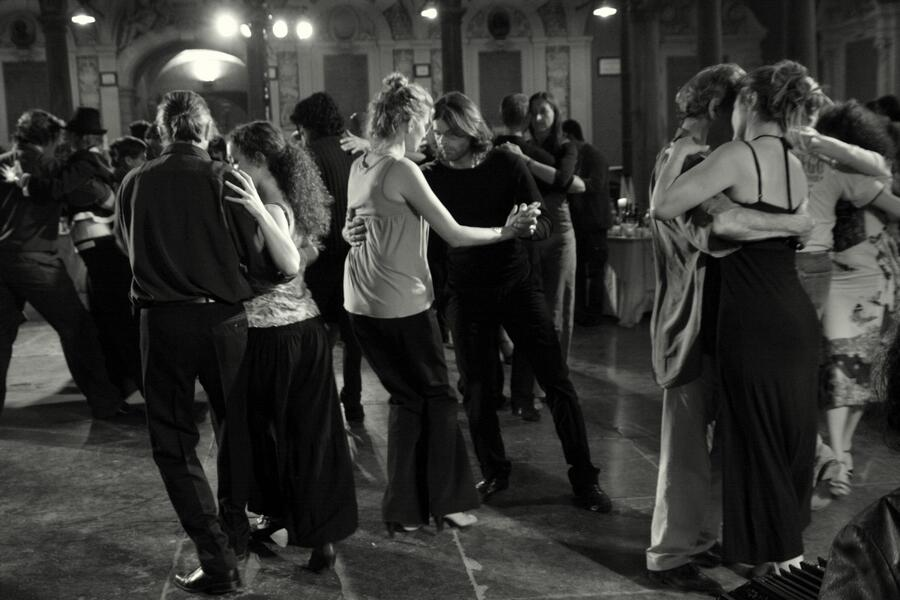
\includegraphics[scale=0.6]{dance/tango-08-39}

\end{center}


\begin{comment}
Advanced features (polling) 
\end{comment}


\chapter{Advanced features}


\section{Attribute alarms}

Each Tango attribute two several alarms. These alarms are :
\begin{itemize}
\item A four thresholds level alarm
\item The read different than set (RDS\index{RDS}) alarm
\end{itemize}

\subsection{The level alarms}

This alarm is defined for all Tango attribute read type and for numerical
data type. The action of this alarm depend on the attribute value
when it is read :
\begin{itemize}
\item If the attribute value is below or equal the attribute configuration
\textbf{min\_alarm\index{min-alarm}} parameter, the attribute quality
factor is switched to Tango::ATTR\_ALARM\index{ATTR-ALARM} and if
the device state is Tango::ON, it is switched to Tango::ALARM. 
\item If the attribute value is below or equal the attribute configuration
\textbf{min\_warning\index{min-warning}} parameter, the attribute
quality factor is switched to Tango::ATTR\_WARNING\index{ATTR-WARNING}
and if the device state is Tango::ON, it is switched to Tango::ALARM.
\item If the attribute value is above or equal the attribute configuration
\textbf{max\_warning\index{max-warning}} parameter, the attribute
quality factor is switched to Tango::ATTR\_WARNING\index{ATTR-WARNING}
and if the device state is Tango::ON, it is switched to Tango::ALARM.
\item If the attribute value is above or equal the attribute configuration
\textbf{max\_alarm\index{max-alarm}} parameter, the attribute quality
factor is switched to Tango::ATTR\_ALARM\index{ATTR-ALARM} and if
the device state is Tango::ON, it is switched to Tango::ALARM.
\end{itemize}
If the attribute is a spectrum or an image, then the alarm is set
if any one of the attribute value satisfies the above criterium. By
default, these four parameters are not defined and no check will be
done.

The following figure is a drawing of attribute quality factor and
device state values function of the the attribute value.

\begin{figure}[H]
\begin{centering}
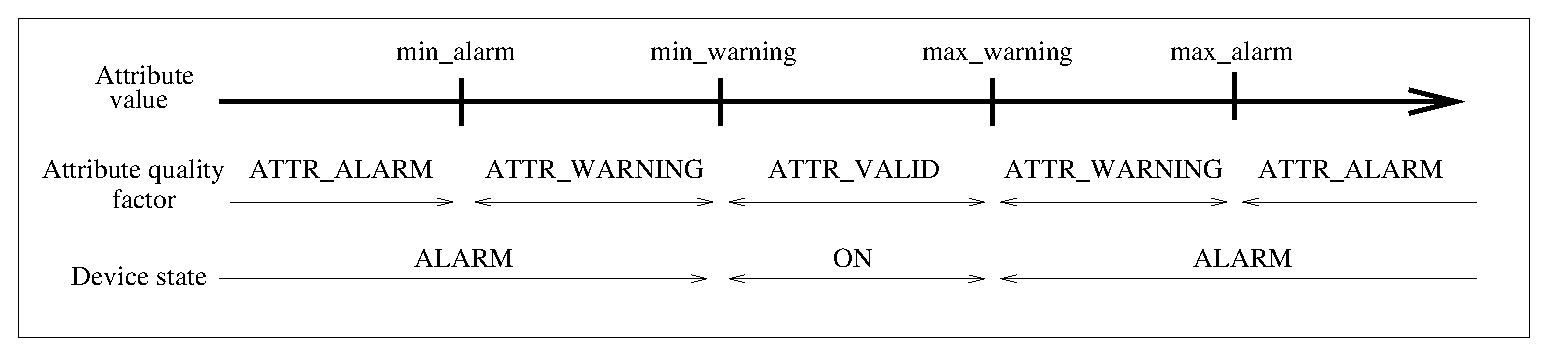
\includegraphics[scale=0.5]{advanced/alarm}
\par\end{centering}

\protect\caption{Level alarm\label{alarm_fig}}
\end{figure}


If the min\_warning and max\_warning parameters are not set, the attribute
quality factor will simply change between Tango::ATTR\_ALARM and Tango::ATTR\_VALID
function of the attribute value.


\subsection{The Read Different than Set (RDS) alarm}

This alarm is defined only for attribute of the Tango::READ\_WRITE
and Tango::READ\_WITH\_WRITE read/write type and for numerical data
type. When the attribute is read (or when the device state is requested),
if the difference between its read value and the last written value
is something more than or equal to an authorized delta and if at least
a certain amount of milli seconds occurs since the last write operation,
the attribute quality factor will be set to Tango::ATTR\_ALARM\index{ATTR-ALARM}
and if the device state is Tango::ON, it is switched to Tango::ALARM\index{ALARM}.
If the attribute is a spectrum or an image, then the alarm is set
if any one of the attribute value's satisfies the above criterium.
This alarm configuration is done with two attribute configuration
parameters called \textbf{delta\_val\index{delta-val}} and \textbf{delta\_t\index{delta-t}}.
By default, these two parameters are not defined and no check will
be done.


\section{Enumerated\index{Enumeration} attribute}

Since Tango release 9, enumerated attribute is supported using the
new data type DevEnum\index{DevEnum}. This data type is not a real
C++ enumeration because:
\begin{enumerate}
\item The enumerated value allways start with 0
\item Values are consecutive
\item It is transferred on the network as DevShort data type
\end{enumerate}
One enumeration label is associated to each enumeration value. For
the Tango kernel, it is this list of enumeration labels which will
define the possible enumeration values. For instance if the enumeration
has 3 labels, its value must be between 0 and 2. There are two ways
to define the enumeration labels:
\begin{enumerate}
\item At attribute creation time. This is the most common case when the
list of possible enumeration values and labels are known at compile
time. The Tango code generator Pogo generates for you the code needed
to pass the enumeration labels to the Tango kernel.
\item In the user code when the enumeration values and labels are not known
at compile time but retrieved during device startup phase. The user
gives the possible enumeration values to the Tango kernel using the
Attribute class \emph{set\_properties()} method.
\end{enumerate}
A Tango client is able to retrieve the enumeration labels in the attribute
configuration returned by instance by a call to the \emph{DeviceProxy::get\_attribute\_config()}
method. Using the \emph{DeviceProxy::set\_attribute\_config()} call,
a user may change the enumeration labels but not their number.


\subsection{Usage in a Tango class}

Within a Tango class, you set the attribute value with a C++ enum
or a DevShort variable. In case a DevShort variable is used, its value
will be checked according to the enumeration labels list given to
Tango kernel.


\subsubsection{Setting the labels with enumeration compile time knowledge}

In such a case, the enumeration labels are given to Tango at the attribute
creation time in the \emph{attribute\_factory} method of the XXXClass
class. Let us take one example

%
% Copyright (C) :      2004,2005,2006,2007,2008,2009,2010,2011,2012,2013
%                      European Synchrotron Radiation Facility
%                      BP 220, Grenoble 38043
%                      FRANCE
%
% This file is part of Tango.
%
% Tango is free software: you can redistribute it and/or modify
% it under the terms of the GNU Lesser General Public License as published by
% the Free Software Foundation, either version 3 of the License, or
% (at your option) any later version.
%
% Tango is distributed in the hope that it will be useful,
% but WITHOUT ANY WARRANTY; without even the implied warranty of
% MERCHANTABILITY or FITNESS FOR A PARTICULAR PURPOSE.  See the
% GNU Lesser General Public License for more details.
%
% You should have received a copy of the GNU Lesser General Public License
% along with Tango.  If not, see <http://www.gnu.org/licenses/>.
%
\begin{flushleft}
\begin{picture}(0,0)
\thicklines
\put(0,0){\line(1,0){400}}
\end{picture}
\end{flushleft}

\begin{lyxcode}
~~~~~1~~enum~class~Card:~short

~~~~~2~~\{

~~~~~3~~~~~~NORTH~=~0,

~~~~~4~~~~~~SOUTH,

~~~~~5~~~~~~EAST,

~~~~~6~~~~~~WEST

~~~~~7~~\};

~~~~~8~

~~~~~9~~void~XXXClass::attribute\_factory(vector<Tango::Attr~{*}>~\&att\_list)

~~~~10~~\{

~~~~11~~~~~~.....

~~~~12~~~~~~TheEnumAttrib	{*}theenum~=~new~TheEnumAttrib();

~~~~13~~~~~~Tango::UserDefaultAttrProp~theenum\_prop;

~~~~14~~~~~~vector<string>~labels~=~\{\textquotedbl{}North\textquotedbl{},\textquotedbl{}South\textquotedbl{},\textquotedbl{}East\textquotedbl{},\textquotedbl{}West\textquotedbl{}\};

~~~~15~~~~~~theenum\_prop.set\_enum\_labels(labels);

~~~~16~~~~~~theenum->set\_default\_properties(theenum\_prop);

~~~~17~~~~~~att\_list.push\_back(theenum);

~~~~18~~~~~~.....

~~~~19~~~\}	
\end{lyxcode}
%
% Copyright (C) :      2004,2005,2006,2007,2008,2009,2010,2011,2012,2013
%                      European Synchrotron Radiation Facility
%                      BP 220, Grenoble 38043
%                      FRANCE
%
% This file is part of Tango.
%
% Tango is free software: you can redistribute it and/or modify
% it under the terms of the GNU Lesser General Public License as published by
% the Free Software Foundation, either version 3 of the License, or
% (at your option) any later version.
%
% Tango is distributed in the hope that it will be useful,
% but WITHOUT ANY WARRANTY; without even the implied warranty of
% MERCHANTABILITY or FITNESS FOR A PARTICULAR PURPOSE.  See the
% GNU Lesser General Public License for more details.
%
% You should have received a copy of the GNU Lesser General Public License
% along with Tango.  If not, see <http://www.gnu.org/licenses/>.
%
\begin{flushleft}
\begin{picture}(0,0)
\thicklines
\put(0,0){\line(1,0){400}}
\end{picture}
\end{flushleft}


line 1-7 : The definition of the enumeration (C++11 in this example)

line 14 : A vector of strings with the enumeration labels is created.
Because there is no way to get the labels from the enumeration definition,
they are re-defined here.

line 15 : This vector is given to the theenum\_prop object which contains
the user default properties

line 16 : The user default properties are associated to the attribute\\


In most cases, all this code will be automatically generated by the
Tango code generator Pogo. It is given here for completness.


\subsubsection{Setting the labels without enumeration compile time knowledge}

In such a case, the enumeration labels are retrieved by the user in
a way specific to the device and passed to Tango using the Attribute
class \emph{set\_properties()} method. Let us take one example

%
% Copyright (C) :      2004,2005,2006,2007,2008,2009,2010,2011,2012,2013
%                      European Synchrotron Radiation Facility
%                      BP 220, Grenoble 38043
%                      FRANCE
%
% This file is part of Tango.
%
% Tango is free software: you can redistribute it and/or modify
% it under the terms of the GNU Lesser General Public License as published by
% the Free Software Foundation, either version 3 of the License, or
% (at your option) any later version.
%
% Tango is distributed in the hope that it will be useful,
% but WITHOUT ANY WARRANTY; without even the implied warranty of
% MERCHANTABILITY or FITNESS FOR A PARTICULAR PURPOSE.  See the
% GNU Lesser General Public License for more details.
%
% You should have received a copy of the GNU Lesser General Public License
% along with Tango.  If not, see <http://www.gnu.org/licenses/>.
%
\begin{flushleft}
\begin{picture}(0,0)
\thicklines
\put(0,0){\line(1,0){400}}
\end{picture}
\end{flushleft}

\begin{lyxcode}
~~~~~1~~void~MyDev::init\_device()

~~~~~2~~\{

~~~~~3~~~~~~...

~~~~~4~~

~~~~~5~~~~~~Attribute~\&att~=~get\_device\_attr()->get\_attr\_by\_name(\textquotedbl{}TheEnumAtt\textquotedbl{});

~~~~~6~~~~~~MultiAttrProp<DevEnum>~multi\_prop;

~~~~~7~~~~~~att.get\_properties(multi\_prop);

~~~~~8~

~~~~~9~~~~~~multi\_prop.enum\_labels~=~\{....\};

~~~~10~~~~~~att.set\_properties(multi\_prop);

~~~~11~~~~~~....

~~~~12~~~\}	
\end{lyxcode}
%
% Copyright (C) :      2004,2005,2006,2007,2008,2009,2010,2011,2012,2013
%                      European Synchrotron Radiation Facility
%                      BP 220, Grenoble 38043
%                      FRANCE
%
% This file is part of Tango.
%
% Tango is free software: you can redistribute it and/or modify
% it under the terms of the GNU Lesser General Public License as published by
% the Free Software Foundation, either version 3 of the License, or
% (at your option) any later version.
%
% Tango is distributed in the hope that it will be useful,
% but WITHOUT ANY WARRANTY; without even the implied warranty of
% MERCHANTABILITY or FITNESS FOR A PARTICULAR PURPOSE.  See the
% GNU Lesser General Public License for more details.
%
% You should have received a copy of the GNU Lesser General Public License
% along with Tango.  If not, see <http://www.gnu.org/licenses/>.
%
\begin{flushleft}
\begin{picture}(0,0)
\thicklines
\put(0,0){\line(1,0){400}}
\end{picture}
\end{flushleft}


line 5 : Get a reference to the attribute object

line 7 : Retrieve the attribute properties

line 9 : Initialise the attribute labels in the set of attribute properties

line 10 : Set the attribute properties


\subsubsection{Setting the attribute value}

It is possible to set the attribute value using either a classical
DevShort variable or using a variable of the C++ enumeration. The
following example is when you have compile time knowledge of the enumeration
definition. We assume that the enumeration is the same than the one
defined above (Card enumeration)

%
% Copyright (C) :      2004,2005,2006,2007,2008,2009,2010,2011,2012,2013
%                      European Synchrotron Radiation Facility
%                      BP 220, Grenoble 38043
%                      FRANCE
%
% This file is part of Tango.
%
% Tango is free software: you can redistribute it and/or modify
% it under the terms of the GNU Lesser General Public License as published by
% the Free Software Foundation, either version 3 of the License, or
% (at your option) any later version.
%
% Tango is distributed in the hope that it will be useful,
% but WITHOUT ANY WARRANTY; without even the implied warranty of
% MERCHANTABILITY or FITNESS FOR A PARTICULAR PURPOSE.  See the
% GNU Lesser General Public License for more details.
%
% You should have received a copy of the GNU Lesser General Public License
% along with Tango.  If not, see <http://www.gnu.org/licenses/>.
%
\begin{flushleft}
\begin{picture}(0,0)
\thicklines
\put(0,0){\line(1,0){400}}
\end{picture}
\end{flushleft}

\begin{lyxcode}
~~~~~1~~enum~Card~points;

~~~~~2~~

~~~~~3~~void~MyDev::read\_TheEnum(Attribute~\&att)

~~~~~4~~\{

~~~~~5~~~~~~...

~~~~~6~~~~~~points~=~SOUTH;

~~~~~7~~~~~~att.set\_value(\&points);

~~~~~8~~\}
\end{lyxcode}
%
% Copyright (C) :      2004,2005,2006,2007,2008,2009,2010,2011,2012,2013
%                      European Synchrotron Radiation Facility
%                      BP 220, Grenoble 38043
%                      FRANCE
%
% This file is part of Tango.
%
% Tango is free software: you can redistribute it and/or modify
% it under the terms of the GNU Lesser General Public License as published by
% the Free Software Foundation, either version 3 of the License, or
% (at your option) any later version.
%
% Tango is distributed in the hope that it will be useful,
% but WITHOUT ANY WARRANTY; without even the implied warranty of
% MERCHANTABILITY or FITNESS FOR A PARTICULAR PURPOSE.  See the
% GNU Lesser General Public License for more details.
%
% You should have received a copy of the GNU Lesser General Public License
% along with Tango.  If not, see <http://www.gnu.org/licenses/>.
%
\begin{flushleft}
\begin{picture}(0,0)
\thicklines
\put(0,0){\line(1,0){400}}
\end{picture}
\end{flushleft}


line 1 : One instance of the Card enum is created (named points)

line 6 : The enumeration is initialized

line 7 : The value of the attribute object is set using the enumeration
(by pointer)\\
To get the same result using a classical DevShort variable, the code
looks like

%
% Copyright (C) :      2004,2005,2006,2007,2008,2009,2010,2011,2012,2013
%                      European Synchrotron Radiation Facility
%                      BP 220, Grenoble 38043
%                      FRANCE
%
% This file is part of Tango.
%
% Tango is free software: you can redistribute it and/or modify
% it under the terms of the GNU Lesser General Public License as published by
% the Free Software Foundation, either version 3 of the License, or
% (at your option) any later version.
%
% Tango is distributed in the hope that it will be useful,
% but WITHOUT ANY WARRANTY; without even the implied warranty of
% MERCHANTABILITY or FITNESS FOR A PARTICULAR PURPOSE.  See the
% GNU Lesser General Public License for more details.
%
% You should have received a copy of the GNU Lesser General Public License
% along with Tango.  If not, see <http://www.gnu.org/licenses/>.
%
\begin{flushleft}
\begin{picture}(0,0)
\thicklines
\put(0,0){\line(1,0){400}}
\end{picture}
\end{flushleft}

\begin{lyxcode}
~~~~~1~~DevShort~sh;

~~~~~2~~

~~~~~3~~void~MyDev::read\_TheEnum(Attribute~\&att)

~~~~~4~~\{

~~~~~5~~~~~~...

~~~~~6~~~~~~sh~=~1;

~~~~~7~~~~~~att.set\_value(\&sh);

~~~~~8~~\}
\end{lyxcode}
%
% Copyright (C) :      2004,2005,2006,2007,2008,2009,2010,2011,2012,2013
%                      European Synchrotron Radiation Facility
%                      BP 220, Grenoble 38043
%                      FRANCE
%
% This file is part of Tango.
%
% Tango is free software: you can redistribute it and/or modify
% it under the terms of the GNU Lesser General Public License as published by
% the Free Software Foundation, either version 3 of the License, or
% (at your option) any later version.
%
% Tango is distributed in the hope that it will be useful,
% but WITHOUT ANY WARRANTY; without even the implied warranty of
% MERCHANTABILITY or FITNESS FOR A PARTICULAR PURPOSE.  See the
% GNU Lesser General Public License for more details.
%
% You should have received a copy of the GNU Lesser General Public License
% along with Tango.  If not, see <http://www.gnu.org/licenses/>.
%
\begin{flushleft}
\begin{picture}(0,0)
\thicklines
\put(0,0){\line(1,0){400}}
\end{picture}
\end{flushleft}


line 1 : A DevShort variable is created (named sh)

line 6 : The variable is initialized

line 7 : The value of the attribute object is set using the DevShort
variable (by pointer)


\subsection{Usage in a Tango client}

Within a Tango client, you insert/extract enumerated attribute value
in/from DeviceAttribute object with a C++ enum or a DevShort variable.
The later case is for generic client which do not have compile time
knowledge of the enumeration. The code looks like

%
% Copyright (C) :      2004,2005,2006,2007,2008,2009,2010,2011,2012,2013
%                      European Synchrotron Radiation Facility
%                      BP 220, Grenoble 38043
%                      FRANCE
%
% This file is part of Tango.
%
% Tango is free software: you can redistribute it and/or modify
% it under the terms of the GNU Lesser General Public License as published by
% the Free Software Foundation, either version 3 of the License, or
% (at your option) any later version.
%
% Tango is distributed in the hope that it will be useful,
% but WITHOUT ANY WARRANTY; without even the implied warranty of
% MERCHANTABILITY or FITNESS FOR A PARTICULAR PURPOSE.  See the
% GNU Lesser General Public License for more details.
%
% You should have received a copy of the GNU Lesser General Public License
% along with Tango.  If not, see <http://www.gnu.org/licenses/>.
%
\begin{flushleft}
\begin{picture}(0,0)
\thicklines
\put(0,0){\line(1,0){400}}
\end{picture}
\end{flushleft}

\begin{lyxcode}
~~~~~1~~DeviceAttribute~da~=~the\_dev.read\_attribute(\textquotedbl{}TheEnumAtt\textquotedbl{});

~~~~~2~~Card~ca;

~~~~~3~~da~>\textcompwordmark{}>~ca;

~~~~~4~~

~~~~~5~~DeviceAttribute~db~=~the\_dev.read\_attribute(\textquotedbl{}TheEnumAtt\textquotedbl{});

~~~~~6~~DevShort~sh;

~~~~~7~~da~>\textcompwordmark{}>~sh;
\end{lyxcode}
%
% Copyright (C) :      2004,2005,2006,2007,2008,2009,2010,2011,2012,2013
%                      European Synchrotron Radiation Facility
%                      BP 220, Grenoble 38043
%                      FRANCE
%
% This file is part of Tango.
%
% Tango is free software: you can redistribute it and/or modify
% it under the terms of the GNU Lesser General Public License as published by
% the Free Software Foundation, either version 3 of the License, or
% (at your option) any later version.
%
% Tango is distributed in the hope that it will be useful,
% but WITHOUT ANY WARRANTY; without even the implied warranty of
% MERCHANTABILITY or FITNESS FOR A PARTICULAR PURPOSE.  See the
% GNU Lesser General Public License for more details.
%
% You should have received a copy of the GNU Lesser General Public License
% along with Tango.  If not, see <http://www.gnu.org/licenses/>.
%
\begin{flushleft}
\begin{picture}(0,0)
\thicklines
\put(0,0){\line(1,0){400}}
\end{picture}
\end{flushleft}


line 2-3 : The attribute value is extracted in a C++ enumeration variable

line 6-7 : The attribute value is extracted in a DevShort variable


\section{Device polling}


\subsection{Introduction}

Each tango device server automatically have a separate polling\index{polling}
thread pool. Polling a device means periodically executing command
on a device (or reading device attribute) and storing the results
(or the thrown exception) in a polling buffer. The aim of this polling
is threefold :
\begin{itemize}
\item Speed-up response time for slow device
\item Get a first-level history of device command output or attribute value
\item Be the data source for the Tango event system
\end{itemize}
Speeding-up response time is achieved because the command\_inout or
read\_attribute CORBA operation is able to get its data from the polling
buffer or from the a real access to the device. For ``slow'' device,
getting the data from the buffer is much faster than accessing the
device. Returning a first-level command output history (or attribute
value history) to a client is possible due to the polling buffer which
is managed as a circular buffer. The history is the contents of this
circular buffer. Obviously, the history depth is limited to the depth
of the circular buffer. The polling is also the data source for the
event system because detecting an event means being able to regularly
read the data, memorize it and declaring that it is an event after
some comparison with older values.

Starting with Tango 9, the default polling algorithm has been modifed.
However, it is still possible to use the polling as it was in Tango
releases prior to release 9. See chaper on polling configuration to
get details on this.


\subsection{Configuring the polling system}


\subsubsection{Configuring what has to be polled and how}

It is possible to configure the polling in order to poll :
\begin{itemize}
\item Any command which does not need input parameter
\item Any attribute
\end{itemize}
Configuring the polling is done by sending command to the device server
administration device automatically implemented in every device server
process. Seven commands are dedicated to this feature. These commands
are
\begin{description}
\item [{AddObjPolling\index{AddObjPolling}}] It add a new object (command
or attribute) to the list of object(s) to be polled. It is also with
this command that the polling period is specified.
\item [{RemObjPolling\index{RemObjPolling}}] To remove one object (command
or attribute) from the polled object(s) list
\item [{UpdObjPollingPeriod\index{UpdObjPollingPeriod}}] Change one object
polling period
\item [{StartPolling\index{StartPolling}}] Starts polling for the whole
process
\item [{StopPolling\index{StopPolling}}] Stops polling for the whole process
\item [{PolledDevice\index{PolledDevice}}] Allow a client to know which
device are polled
\item [{DevPollStatus\index{DevPollStatus}}] Allow a client to precisely
knows the polling status for a device
\end{description}
All the necessary parameters for the polling configuration are stored
in the Tango database. Therefore, the polling configuration is not
lost after a device server process stop and restart (or after a device
server process crash!!).

It is also possible to automatically poll a command (or an attribute)
without sending command to the device server administration device.
This request some coding (a method call) in the device server software
during the command or attribute creation. In this case, for every
devices supporting this command or this attribute, polling configuration
will be automatically updated in the database and the polling will
start automatically at each device server process startup. It is possible
to stop this behavior on a device basis by sending a RemObjPolling\index{RemObjPolling}
command to the device server administration device. The following
piece of code shows how the source code should be written.

%
% Copyright (C) :      2004,2005,2006,2007,2008,2009,2010,2011,2012,2013
%                      European Synchrotron Radiation Facility
%                      BP 220, Grenoble 38043
%                      FRANCE
%
% This file is part of Tango.
%
% Tango is free software: you can redistribute it and/or modify
% it under the terms of the GNU Lesser General Public License as published by
% the Free Software Foundation, either version 3 of the License, or
% (at your option) any later version.
%
% Tango is distributed in the hope that it will be useful,
% but WITHOUT ANY WARRANTY; without even the implied warranty of
% MERCHANTABILITY or FITNESS FOR A PARTICULAR PURPOSE.  See the
% GNU Lesser General Public License for more details.
%
% You should have received a copy of the GNU Lesser General Public License
% along with Tango.  If not, see <http://www.gnu.org/licenses/>.
%
\begin{flushleft}
\begin{picture}(0,0)
\thicklines
\put(0,0){\line(1,0){400}}
\end{picture}
\end{flushleft}

\begin{lyxcode}
~~~~~1~~

~~~~~2~~void~DevTestClass::command\_factory()

~~~~~3~~\{

~~~~~4~~...

~~~~~5~~~~~~command\_list.push\_back(new~IOStartPoll(\textquotedbl{}IOStartPoll\textquotedbl{},

~~~~~6~~~~~~~~~~~~~~~~~~~~~~~~~~~~~~~~~~~~~~~~~~~~~~Tango::DEV\_VOID,

~~~~~7~~~~~~~~~~~~~~~~~~~~~~~~~~~~~~~~~~~~~~~~~~~~~~Tango::DEV\_LONG,

~~~~~8~~~~~~~~~~~~~~~~~~~~~~~~~~~~~~~~~~~~~~~~~~~~~~\textquotedbl{}Void\textquotedbl{},

~~~~~9~~~~~~~~~~~~~~~~~~~~~~~~~~~~~~~~~~~~~~~~~~~~~~\textquotedbl{}Constant~number\textquotedbl{}));

~~~~10~~~~~~command\_list.back()->set\_polling\_period(400);

~~~~11~~...

~~~~12~~\}

~~~~13~~

~~~~14~~

~~~~15~~void~DevTestClass::attribute\_factory(vector<Tango::Attr~{*}>~\&att\_list)

~~~~16~~\{

~~~~17~~...

~~~~18~~~~~~att\_list.push\_back(new~Tango::Attr(\textquotedbl{}String\_attr\textquotedbl{},

~~~~19~~~~~~~~~~~~~~~~~~~~~~~~~~~~~~~~~~~~~~~~~~Tango::DEV\_STRING,

~~~~20~~~~~~~~~~~~~~~~~~~~~~~~~~~~~~~~~~~~~~~~~~Tango::READ));

~~~~21~~~~~~att\_list.back()->set\_polling\_period(250);

~~~~22~~...

~~~~23~~\}
\end{lyxcode}
%
% Copyright (C) :      2004,2005,2006,2007,2008,2009,2010,2011,2012,2013
%                      European Synchrotron Radiation Facility
%                      BP 220, Grenoble 38043
%                      FRANCE
%
% This file is part of Tango.
%
% Tango is free software: you can redistribute it and/or modify
% it under the terms of the GNU Lesser General Public License as published by
% the Free Software Foundation, either version 3 of the License, or
% (at your option) any later version.
%
% Tango is distributed in the hope that it will be useful,
% but WITHOUT ANY WARRANTY; without even the implied warranty of
% MERCHANTABILITY or FITNESS FOR A PARTICULAR PURPOSE.  See the
% GNU Lesser General Public License for more details.
%
% You should have received a copy of the GNU Lesser General Public License
% along with Tango.  If not, see <http://www.gnu.org/licenses/>.
%
\begin{flushleft}
\begin{picture}(0,0)
\thicklines
\put(0,0){\line(1,0){400}}
\end{picture}
\end{flushleft}


A polling period of 400 mS is set for the command called ``IOStartPoll''
at line 10 with the \emph{set\_polling\_period} method of the Command
class. Therefore, for a device of this class, the polling thread will
start polling its IOStartPoll command at process start-up except if
a RemObjPolling indicating this device and the IOStartPoll command
has already been received by the device server administration device.
This is exactly the same behavior for attribute. The polling period
for attribute called ``String\_attr'' is defined at line 20.

Configuring the polling means defining device attribute/command polling
period. The polling period has to be chosen with care. If reading
an attribute needs 200 mS, there is no point to poll this attribute
with a polling period equal or even below 200 mS. You should also
take into account that some \textquotedbl{}free\textquotedbl{} time
has to be foreseen for external request(s) on the device. On average,
for one attribute needing X mS as reading time, define a polling period
which is equal to 1.4 X (280 mS for our example of one attribute needing
200 mS as reading time). In case the polling tuning is given to external
user, Tango provides a way to define polling period minimun threshold.
This is done using device properties. These properties are named \emph{min\_poll\_period},
\emph{cmd\_min\_poll\_period} and \emph{attr\_min\_poll\_period}.
The property min\_poll\_period\index{min-poll-period} (mS) defined
a minimun polling period for the device. The property cmd\_min\_poll\_period\index{cmd-min-poll-period}
allows the definition of a minimun polling period for a specific device
command. The property attr\_min\_poll\_period\index{attr-min-poll-period}
allows the definition of a minimun polling period for one device attribute.
In case these properties are defined, it is not possible to poll the
device command/attribute with a polling period below those defined
by these properties. See Appendix A on device parameter to get a precise
syntax description for these properties.

The Jive\cite{Jive doc} tool also allows a graphical device polling
configuration.


\subsubsection{Configuring the polling threads pool}

Starting with Tango release 7, a Tango device server process may have
several polling threads managed as a pool. For instance, this could
be usefull in case of devices within the same device server process
but accessed by different hardware channel when one of the channel
is not responding (Thus generating long timeout and de-synchronising
the polling thread). By default, the polling threads pool size is
set to 1 and all the polled object(s) are managed by the same thread
(idem polling system in Tango releases older than release 7) . The
configuration of the polling thread pool is done using two properties
associated to the device server administration device. These properties
are named:
\begin{itemize}
\item \emph{polling\_threads\_pool\_size\index{polling-threads-pool-size}}
defining the maximun number of threads that you can have in the pool
\item \emph{polling\_threads\_pool\_conf\index{polling-threads-pool-conf}}
defining which threads in the pool manages which device
\end{itemize}
The granularity of the polling threads pool tuning is the device.
You cannot ask the polling threads pool to have thread number 1 in
charge of attribute \emph{att1} of device \emph{dev1} and thread number
2 to be in charge of \emph{att2} of the same device \emph{dev1}.

When you require a new object (command or attribute) to be polled,
two main cases may arrive:
\begin{enumerate}
\item Some polled object(s) belonging to the device are already polled by
one of the polling threads in the pool: There is no new thread created.
The object is simply added to the list of objects to be polled for
the existing thread
\item There is no thread already created for the device. We have two sub-cases:

\begin{enumerate}
\item The number of polling threads is less than the polling\_threads\_pool\_size:
A new thread is created and started to poll the object (command or
attribute)
\item The number of polling threads is already equal to the polling\_threads\_pool\_size:
The software search for the thread with the smallest number of polled
objects and add the new polled object to this thread
\end{enumerate}
\end{enumerate}
Each time the polling threads pool configuration is changed, it is
written in the database using the polling\_threads\_pool\_conf property.
If the behaviour previously described does not fulfill your needs,
it is possible to update the polling\_threads\_pool\_conf property
in a graphical way using the Tango Astor \cite{Astor_doc} tool or
manually using the Jive tool \cite{Jive doc}. These changes will
be taken into account at the next device server process start-up.
At start-up, the polling threads pool will allways be configured as
required by the polling\_threads\_pool\_conf property. The syntax
used for this property is described in the Reference part of the Appendix
\ref{cha:Reference-part}. The following window dump is the Astor
tool window which allows polling threads pool management.\begin{center}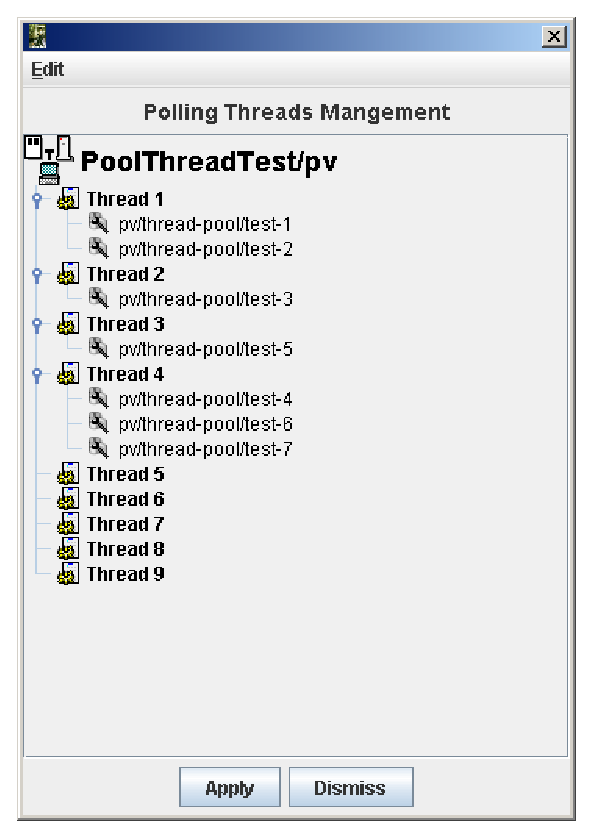
\includegraphics{advanced/ThreadsManagement}\end{center}

In this example, the polling threads pool size to set to 9 but only
4 polling threads are running. Thread 1 is in charge of all polled
objects related to device pv/thread-pool/test-1 and pv/thread-pool/test-2.
Thread 2 is in charge of all polled objects related to device pv/thread-pool/test-3.
Thread 3 is in charge of all polled objects related to device pv/thread-pool/test-5
anf finally, thread 4 is in charge of all polled objects for devices
pv/thread-pool/test-4, pv/thread-pool/test-6 and pv/thread-pool/test-7.

It's also possible to define the polling threads pool size programmatically
in the main function of a device server process using the \emph{Util::set\_polling\_threads\_pool\_size()\index{set-polling-threads-pool-size}}
method before the call to the \emph{Util::server\_init()} method


\subsubsection{Choosing polling algorithm}

Starting with Tango 9, you can choose between two different polling
algorithm:
\begin{itemize}
\item The polling as it was in Tango since it has been introduced. This
means:

\begin{itemize}
\item For one device, always poll attribute one at a time even if the polling
period is the same (use of read\_attribute instead of read\_attributes)
\item Do not allow the polling thread to be late: If it is the case (because
at the end of polling object 1, the time is greater than the polling
date of object 2), discard polling object and inform event user by
sending one event with error (Polling thread is late and discard....)
\end{itemize}
\item New polling algorithm introduced in Tango 9 as the default one. This
means:

\begin{itemize}
\item For one device, poll all attributes with the same polling period using
a single device call (read\_attributes)
\item Allow the polling thread to be late but only if number of late objects
decreases.
\end{itemize}
\end{itemize}
The advantages of new polling algorithm are 
\begin{enumerate}
\item In case of several attributes polled on the same device at the same
period a lower device occupation time by the polling thread (due to
a single read\_attributes() call instead of several single read\_attribute()
calls)
\item Less ``Polling thread late'' errors in the event system in case
of device with non constant response time
\end{enumerate}
The drawback is
\begin{enumerate}
\item The loss of attribute individual timing data reported in the polling
thread status
\end{enumerate}
It is still possible to return to pre-release 9 polling algorithm.
To do so, you can use the device server process administration device
\emph{polling\_before\_9}\index{polling_before_9@polling\_before\_9}
property by setting it to true. It is also possible to choose this
pre-release 9 algorithm in device server process code in the main
function of the process using the \emph{Util::set\_polling\_before\_9()}
method.


\subsection{Reading data from the polling buffer}

For a polled command or a polled attribute, a client has three possibilities
to get command result or attribute value (or the thrown exception)
:
\begin{itemize}
\item From the device itself
\item From the polling buffer
\item From the polling buffer first and from the device if data in the polling
buffer are invalid or if the polling is badly configured.
\end{itemize}
The choice is done during the command\_inout CORBA operation by positioning
one of the operation parameter. When reading data from the polling
buffer, several error cases are possible 
\begin{itemize}
\item The data in the buffer are not valid any more. Every time data are
requested from the polling buffer, a check is done between the client
request date and the date when the data were stored in the buffer.
An exception is thrown if the delta is greater than the polling period
multiplied by a ``too old'' factor. This factor has a default value
and is up-datable via a device property. This is detailed in the reference
part of this manual.
\item The polling is correctly configured but there is no data yet in the
polling buffer.
\end{itemize}

\subsection{Retrieving command/attribute result history}

The polling thread stores the command result or attribute value in
circular buffers. It is possible to retrieve an history of the command
result (or attribute value) from these polling buffers. Obviously
the history is limited by the depth of the circular buffer. For commands,
a CORBA operation called \emph{command\_inout\_history\_2\index{command-inout-history-2}}
allows this retrieval. The client specifies the command name and the
record number he want to retrieve. For each record, the call returns
the date when the command was executed, the command result or the
exception stack in case of the command failed when it was executed
by the polling thread. In such a case, the exception stack is sent
as a structure member and not as an exception. The same thing is available
for attribute. The CORBA operation name is \emph{read\_attribute\_history\_2\index{read-attribute-history-2}.}
For these two calls, there is no check done between the call date
and the record date in contrary of the call to retrieve the last command
result (or attribute value).


\subsection{Externally triggered polling}

Sometimes, rather than polling a command or an attribute regulary
with a fixed period, it is more interesting to \textquotedbl{}manually\textquotedbl{}
decides when the polling must occurs. The Tango polling system also
supports this kind of usage. This is called \emph{externally triggered
polling}. To define one attribute (or command) as externally triggered,
simply set its polling period to 0. This can be done with the device
server administration device AddObjPolling or UpdObjPollingPeriod
command. Once in this mode, the attribute (or command) polling is
triggered with the \emph{trigger\_cmd\_polling()} method (or \emph{trigger\_attr\_polling()}
method) of the Util class. The following piece of code shows how this
method could be used for one externally triggered command.

%
% Copyright (C) :      2004,2005,2006,2007,2008,2009,2010,2011,2012,2013
%                      European Synchrotron Radiation Facility
%                      BP 220, Grenoble 38043
%                      FRANCE
%
% This file is part of Tango.
%
% Tango is free software: you can redistribute it and/or modify
% it under the terms of the GNU Lesser General Public License as published by
% the Free Software Foundation, either version 3 of the License, or
% (at your option) any later version.
%
% Tango is distributed in the hope that it will be useful,
% but WITHOUT ANY WARRANTY; without even the implied warranty of
% MERCHANTABILITY or FITNESS FOR A PARTICULAR PURPOSE.  See the
% GNU Lesser General Public License for more details.
%
% You should have received a copy of the GNU Lesser General Public License
% along with Tango.  If not, see <http://www.gnu.org/licenses/>.
%
\begin{flushleft}
\begin{picture}(0,0)
\thicklines
\put(0,0){\line(1,0){400}}
\end{picture}
\end{flushleft}

\begin{lyxcode}
~~~~~1~~.....

~~~~~2~~

~~~~~3~~string~ext\_polled\_cmd(\textquotedbl{}MyCmd\textquotedbl{});

~~~~~4~~Tango::DeviceImpl~{*}device~=~.....;

~~~~~5~~

~~~~~6~~Tango::Util~{*}tg~=~Tango::Util::instance();

~~~~~7~~

~~~~~8~~tg->trigger\_cmd\_polling(device,ext\_polled\_cmd);

~~~~~9~~

~~~~10~~.....


\end{lyxcode}
%
% Copyright (C) :      2004,2005,2006,2007,2008,2009,2010,2011,2012,2013
%                      European Synchrotron Radiation Facility
%                      BP 220, Grenoble 38043
%                      FRANCE
%
% This file is part of Tango.
%
% Tango is free software: you can redistribute it and/or modify
% it under the terms of the GNU Lesser General Public License as published by
% the Free Software Foundation, either version 3 of the License, or
% (at your option) any later version.
%
% Tango is distributed in the hope that it will be useful,
% but WITHOUT ANY WARRANTY; without even the implied warranty of
% MERCHANTABILITY or FITNESS FOR A PARTICULAR PURPOSE.  See the
% GNU Lesser General Public License for more details.
%
% You should have received a copy of the GNU Lesser General Public License
% along with Tango.  If not, see <http://www.gnu.org/licenses/>.
%
\begin{flushleft}
\begin{picture}(0,0)
\thicklines
\put(0,0){\line(1,0){400}}
\end{picture}
\end{flushleft}


line 3 : The externally polled command name

line 4 : The device object

line 8 : Trigger polling of command MyCmd


\subsection{Filling polling buffer}

Some hardware to be interfaced already returned an array of pair value,
timestamp. In order to be read with the \emph{command\_inout\_history}
or \emph{read\_attribute\_history} calls, this array has to be transferred
in the attribute or command polling buffer. This is possible only
for attribute or command configured in the externally triggered polling
mode. Once in externally triggered polling mode, the attribute (or
command) polling buffer is filled with the \emph{fill\_cmd\_polling\_buffer()\index{fill-cmd-polling-buffer}}
method (or \emph{fill\_attr\_polling\_buffer()\index{fill-attr-polling-buffer}}
method) of the Util class. For command, the user uses a template class
called \emph{TimedCmdData\index{TimedCmdData}} for each element of
the command history. Each element is stored in a stack in one instance
of a template class called \emph{CmdHistoryStack\index{CmdHistoryStack}.}
This object is one of the argument of the fill\_cmd\_polling\_buffer()
method. Obviously, the stack depth cannot be larger than the polling
buffer depth. See \ref{sub:The-device-polling-prop} to learn how
the polling buffer depth is defined. The same way is used for attribute
with the \emph{TimedAttrData\index{TimedAttrData}} and \emph{AttrHistoryStack\index{AttrHistoryStack}}
template classes. These classes are documented in \cite{TANGO_ref_man}.
The following piece of code fills the polling buffer for a command
called MyCmd which is already in externally triggered mode. It returns
a DevVarLongArray data type with three elements. This example is not
really something you will find in a real hardware interface. It is
only to demonstrate the fill\_cmd\_polling\_buffer() method usage.
Error management has also been removed.

%
% Copyright (C) :      2004,2005,2006,2007,2008,2009,2010,2011,2012,2013
%                      European Synchrotron Radiation Facility
%                      BP 220, Grenoble 38043
%                      FRANCE
%
% This file is part of Tango.
%
% Tango is free software: you can redistribute it and/or modify
% it under the terms of the GNU Lesser General Public License as published by
% the Free Software Foundation, either version 3 of the License, or
% (at your option) any later version.
%
% Tango is distributed in the hope that it will be useful,
% but WITHOUT ANY WARRANTY; without even the implied warranty of
% MERCHANTABILITY or FITNESS FOR A PARTICULAR PURPOSE.  See the
% GNU Lesser General Public License for more details.
%
% You should have received a copy of the GNU Lesser General Public License
% along with Tango.  If not, see <http://www.gnu.org/licenses/>.
%
\begin{flushleft}
\begin{picture}(0,0)
\thicklines
\put(0,0){\line(1,0){400}}
\end{picture}
\end{flushleft}

\begin{lyxcode}
~~~~~1~~....

~~~~~2~~

~~~~~3~~Tango::DevVarLongArray~dvla\_array{[}4{]};

~~~~~4~~~~~~~~~~

~~~~~5~~for(int~i~=~0;i~<~4;i++)

~~~~~6~~\{

~~~~~7~~~~~~dvla\_array{[}i{]}.length(3);

~~~~~8~~~~~~dvla\_array{[}i{]}{[}0{]}~=~10~+~i;

~~~~~9~~~~~~dvla\_array{[}i{]}{[}1{]}~=~11~+~i;

~~~~10~~~~~~dvla\_array{[}i{]}{[}2{]}~=~12~+~i;

~~~~11~~\}

~~~~12~~

~~~~13~~Tango::CmdHistoryStack<DevVarLongArray>~chs;

~~~~14~~chs.length(4);

~~~~15~~

~~~~16~~for~(int~k~=~0;k~<~4;k++)

~~~~17~~\{

~~~~18~~~~~~time\_t~when~=~time(NULL);

~~~~19~~

~~~~20~~~~~~Tango::TimedCmdData<DevVarLongArray>~tcd(\&dvla\_array{[}k{]},when);

~~~~21~~~~~~chs.push(tcd);

~~~~22~~\}

~~~~23~~

~~~~24~~Tango::Util~{*}tg~=~Tango::Util::instance();

~~~~25~~string~cmd\_name(\textquotedbl{}MyCmd\textquotedbl{});

~~~~26~~DeviceImpl~{*}dev~=~....;

~~~~27~~

~~~~28~~tg->fill\_cmd\_polling\_buffer(dev,cmd\_name,chs);

~~~~29~~

~~~~30~~.....


\end{lyxcode}
%
% Copyright (C) :      2004,2005,2006,2007,2008,2009,2010,2011,2012,2013
%                      European Synchrotron Radiation Facility
%                      BP 220, Grenoble 38043
%                      FRANCE
%
% This file is part of Tango.
%
% Tango is free software: you can redistribute it and/or modify
% it under the terms of the GNU Lesser General Public License as published by
% the Free Software Foundation, either version 3 of the License, or
% (at your option) any later version.
%
% Tango is distributed in the hope that it will be useful,
% but WITHOUT ANY WARRANTY; without even the implied warranty of
% MERCHANTABILITY or FITNESS FOR A PARTICULAR PURPOSE.  See the
% GNU Lesser General Public License for more details.
%
% You should have received a copy of the GNU Lesser General Public License
% along with Tango.  If not, see <http://www.gnu.org/licenses/>.
%
\begin{flushleft}
\begin{picture}(0,0)
\thicklines
\put(0,0){\line(1,0){400}}
\end{picture}
\end{flushleft}


Line 3-11 : Simulate data coming from hardware

Line 13-14 : Create one instance of the CmdHistoryStack class and
reserve space for one history of 4 elements

Line 16-17 : A loop on each history element

Line 18 : Get date (hardware simulation)

Line 20 : Create one instance of the TimedCmdData class with data
and date

Line 21 : Store this command history element in the history stack.
The element order will be the insertion order whatever the element
date is.

Line 28 : Fill command polling buffer

After one execution of this code, a command\_inout\_history() call
will return one history with 4 elements. The first array element of
the oldest history record will have the value 10. The first array
element of the newest history record will have the value 13. A command\_inout()
call with the data source parameter set to CACHE will return the newest
history record (ie an array with values 13,14 and 15). A command\_inout()
call with the data source parameter set to DEVICE will return what
is coded is the command method. If you execute this code a second
time, a command\_inout\_history() call will return an history of 8
elements.

The next example fills the polling buffer for an attribute called
MyAttr which is already in externally triggered mode. It is a scalar
attribute of the DevString data type. This example is not really something
you will find in a real hardware interface. It is only to demonstrate
the fill\_attr\_polling\_buffer() method usage with memory management
issue. Error management has also been removed.

%
% Copyright (C) :      2004,2005,2006,2007,2008,2009,2010,2011,2012,2013
%                      European Synchrotron Radiation Facility
%                      BP 220, Grenoble 38043
%                      FRANCE
%
% This file is part of Tango.
%
% Tango is free software: you can redistribute it and/or modify
% it under the terms of the GNU Lesser General Public License as published by
% the Free Software Foundation, either version 3 of the License, or
% (at your option) any later version.
%
% Tango is distributed in the hope that it will be useful,
% but WITHOUT ANY WARRANTY; without even the implied warranty of
% MERCHANTABILITY or FITNESS FOR A PARTICULAR PURPOSE.  See the
% GNU Lesser General Public License for more details.
%
% You should have received a copy of the GNU Lesser General Public License
% along with Tango.  If not, see <http://www.gnu.org/licenses/>.
%
\begin{flushleft}
\begin{picture}(0,0)
\thicklines
\put(0,0){\line(1,0){400}}
\end{picture}
\end{flushleft}

\begin{lyxcode}
~~~~~1~~....

~~~~~2~~

~~~~~3~~AttrHistoryStack<DevString>~ahs;

~~~~~4~~ahs.length(3);

~~~~~5~~

~~~~~6~~for~(int~k~=~0;k~<~3;k++)

~~~~~7~~\{

~~~~~8~~~~~~time\_t~when~=~time(NULL);

~~~~~9~~

~~~~10~~~~~~DevString~{*}ptr~=~new~DevString~{[}1{]};

~~~~11~~~~~~ptr~=~CORBA::string\_dup(\textquotedbl{}Attr~history~data\textquotedbl{});

~~~~12~~

~~~~13~~~~~~TimedAttrData<DevString>~tad(ptr,Tango::ATTR\_VALID,true,when);

~~~~14~~~~~~ahs.push(tad);

~~~~15~~\}

~~~~16~~

~~~~17~~Tango::Util~{*}tg~=~Tango::Util::instance();

~~~~18~~string~attr\_name(\textquotedbl{}MyAttr\textquotedbl{});

~~~~19~~DeviceImpl~{*}dev~=~....;

~~~~20~~

~~~~21~~tg->fill\_attr\_polling\_buffer(dev,attr\_name,ahs);

~~~~22~~

~~~~23~~.....

~~
\end{lyxcode}
%
% Copyright (C) :      2004,2005,2006,2007,2008,2009,2010,2011,2012,2013
%                      European Synchrotron Radiation Facility
%                      BP 220, Grenoble 38043
%                      FRANCE
%
% This file is part of Tango.
%
% Tango is free software: you can redistribute it and/or modify
% it under the terms of the GNU Lesser General Public License as published by
% the Free Software Foundation, either version 3 of the License, or
% (at your option) any later version.
%
% Tango is distributed in the hope that it will be useful,
% but WITHOUT ANY WARRANTY; without even the implied warranty of
% MERCHANTABILITY or FITNESS FOR A PARTICULAR PURPOSE.  See the
% GNU Lesser General Public License for more details.
%
% You should have received a copy of the GNU Lesser General Public License
% along with Tango.  If not, see <http://www.gnu.org/licenses/>.
%
\begin{flushleft}
\begin{picture}(0,0)
\thicklines
\put(0,0){\line(1,0){400}}
\end{picture}
\end{flushleft}


Line 3-4 : Create one instance of the AttrHistoryStack class and reserve
space for an history with 3 elements

Line 6-7 : A loop on each history element

Line 8 : Get date (hardware simulation)

Line 10-11 : Create a string. Note that the DevString object is created
on the heap

Line 13 : Create one instance of the TimedAttrData class with data
and date requesting the memory to be released.

Line 14 : Store this attribute history element in the history stack.
The element order will be the insertion order whatever the element
date is.

Line 21 : Fill command polling buffer

It is not necessary to return the memory allocated at line 10. The
\emph{fill\_attr\_polling\_buffer()} method will do it for you.


\subsection{Setting and tuning the polling in a Tango class}

Even if the polling is normally set and tuned with external tool like
Jive, it is possible to set it directly into the code of a Tango class.
A set of methods belonging to the \emph{DeviceImpl} class allows the
user to deal with polling. These methods are:
\begin{itemize}
\item \emph{is\_attribute\_polled()} and \emph{is\_command\_polled()} to
check if one command/attribute is polled
\item \emph{get\_attribute\_poll\_period()} and \emph{get\_command\_poll\_period()}
to get polled object polling period
\item \emph{poll\_attribute()} and \emph{poll\_command()} to poll command
or attribute
\item \emph{stop\_poll\_attribute()} and \emph{stop\_poll\_command()} to
stop polling a command or an attribute
\end{itemize}
The following code snippet is just an exmaple of how these methods
could be used. They are documented in \cite{Tango-dsclasses-doc}

%
% Copyright (C) :      2004,2005,2006,2007,2008,2009,2010,2011,2012,2013
%                      European Synchrotron Radiation Facility
%                      BP 220, Grenoble 38043
%                      FRANCE
%
% This file is part of Tango.
%
% Tango is free software: you can redistribute it and/or modify
% it under the terms of the GNU Lesser General Public License as published by
% the Free Software Foundation, either version 3 of the License, or
% (at your option) any later version.
%
% Tango is distributed in the hope that it will be useful,
% but WITHOUT ANY WARRANTY; without even the implied warranty of
% MERCHANTABILITY or FITNESS FOR A PARTICULAR PURPOSE.  See the
% GNU Lesser General Public License for more details.
%
% You should have received a copy of the GNU Lesser General Public License
% along with Tango.  If not, see <http://www.gnu.org/licenses/>.
%
\begin{flushleft}
\begin{picture}(0,0)
\thicklines
\put(0,0){\line(1,0){400}}
\end{picture}
\end{flushleft}

\begin{lyxcode}
~~~~~\lstinputlisting[language={C++}]{advanced/poll_in_ds.cpp.lines}
\end{lyxcode}
%
% Copyright (C) :      2004,2005,2006,2007,2008,2009,2010,2011,2012,2013
%                      European Synchrotron Radiation Facility
%                      BP 220, Grenoble 38043
%                      FRANCE
%
% This file is part of Tango.
%
% Tango is free software: you can redistribute it and/or modify
% it under the terms of the GNU Lesser General Public License as published by
% the Free Software Foundation, either version 3 of the License, or
% (at your option) any later version.
%
% Tango is distributed in the hope that it will be useful,
% but WITHOUT ANY WARRANTY; without even the implied warranty of
% MERCHANTABILITY or FITNESS FOR A PARTICULAR PURPOSE.  See the
% GNU Lesser General Public License for more details.
%
% You should have received a copy of the GNU Lesser General Public License
% along with Tango.  If not, see <http://www.gnu.org/licenses/>.
%
\begin{flushleft}
\begin{picture}(0,0)
\thicklines
\put(0,0){\line(1,0){400}}
\end{picture}
\end{flushleft}



\section{Threading\label{sec:Threading}}

When used with C++, Tango used omniORB as underlying ORB. This CORBA
implementation is a threaded implementation and therefore a C++ Tango
device server or client are multi-threaded processes.


\subsection{Device server process}

A classical Tango device server without any connected clients has
eight threads. These threads\index{thread} are :
\begin{itemize}
\item The main thread waiting in the ORB main loop
\item Two ORB implementation threads (the POA thread)
\item The ORB scavanger thread
\item The signal thread
\item The heartbeat thread (needed by the Tango event system)
\item Two Zmq implementation threads
\end{itemize}
On top of these eight threads, you have to add the thread(s) used
by the polling threads pool. This number depends on the polling thread
pool configuration and could be between 0 (no polling at all) and
the maximun number of threads in the pool.

A new thread is started for each connected client. Device server are
mostly used to interface hardware which most of the time does not
support multi-threaded access. Therefore, all remote calls executed
from a client are serialized within the device server code by using
mutual exclusion. See chapter \ref{sub:Serialization-model-within}
on which serialization model are available. In order to limit thread
number, the underlying ORB (omniORB) is configured to shutdown threads
dedicated to client if the connection is inactive for more than 3
minutes. To also limit thread number, the ORB is configured to create
one thread per connection up to 55 threads. When this level is reached,
the threading model is automatically switch to a \textquotedbl{}thread
pool\textquotedbl{} model with up to 100 threads. If the number of
threads decrease down to 50, the threading model will return to \textquotedbl{}thread
per connection\textquotedbl{} model.

If you are using event, the event system for its internal heartbeat
system periodically (every 200 seconds) sends a command to the device
server administration device. As explained above, a thread is created
to execute these command. The omniORB scavanger will terminate this
thread before the next event system heartbeat command arrives. For
example, if you have a device server with three connected clients
using only event, the process thread number will permanently change
between 8 and 11 threads.

In summary, the number of threads in a device server process can be
evaluated with the following formula:\begin{center}\textbf{8 + k
+ m}\end{center}k is the number of polling threads used from the
polling threads pool and m is the number of threads used for connected
clients.


\subsubsection{Serialization model within a device server\label{sub:Serialization-model-within}}

Four serialization\index{serialization} models are available within
a device server. These models protect all requests coming from the
network but also requests coming from the polling thread. These models
are:
\begin{enumerate}
\item Serialization by device. All access to the same device are serialized.
As an example, let's take a device server implementing one class of
device with two instances (dev1 and dev2). Two clients are connected
to these devices (client1 and client2). Client2 will not be able to
access dev1 if client1 is using it. Nevertheless, client2 is able
to access dev2 while client1 access dev1 (There is one mutual exclusion
object by device)
\item Serialization by class. With non multi-threaded legacy software, the
preceding scenario could generate problem. In this mode of serialization,
client2 is not able to access dev2 while client1 access dev1 because
dev2 and dev1 are instances of the same class (There is one mutual
exclusion object by class)
\item Serialization by process. This is one step further than the previous
case. In this mode, only one client can access any device embedded
within the device server at a time. There is only one mutual exclusion
object for the whole process)
\item No serialization. This is an exotic kind of serialization and \textbf{should
be used with extreme care} only with device which are fully thread
safe. In this model, most of the device access are not serialized
at all. Due to Tango internal structure, the \emph{get\_attribute\_config},
\emph{set\_attribute\_config}, \emph{read\_attributes} and \emph{write\_attributes}
CORBA calls are still protected. Reading the device state and status
via commands or via CORBA attribute is also protected.
\end{enumerate}
By default, every Tango device server is in serialization by device
mode. A method of the Tango::Util class allows to change this default
behavior.\newpage{}

%
% Copyright (C) :      2004,2005,2006,2007,2008,2009,2010,2011,2012,2013
%                      European Synchrotron Radiation Facility
%                      BP 220, Grenoble 38043
%                      FRANCE
%
% This file is part of Tango.
%
% Tango is free software: you can redistribute it and/or modify
% it under the terms of the GNU Lesser General Public License as published by
% the Free Software Foundation, either version 3 of the License, or
% (at your option) any later version.
%
% Tango is distributed in the hope that it will be useful,
% but WITHOUT ANY WARRANTY; without even the implied warranty of
% MERCHANTABILITY or FITNESS FOR A PARTICULAR PURPOSE.  See the
% GNU Lesser General Public License for more details.
%
% You should have received a copy of the GNU Lesser General Public License
% along with Tango.  If not, see <http://www.gnu.org/licenses/>.
%
\begin{flushleft}
\begin{picture}(0,0)
\thicklines
\put(0,0){\line(1,0){400}}
\end{picture}
\end{flushleft}

\begin{lyxcode}
~~~~~1~~\#include~<tango.h>

~~~~~2~~

~~~~~3~~int~main(int~argc,char~{*}argv{[}{]})

~~~~~4~~\{

~~~~~5~~

~~~~~6~~~~~~try

~~~~~7~~~~~~\{

~~~~~8~~~~~~~~~~

~~~~~9~~~~~~~~~~Tango::Util~{*}tg~=~Tango::Util::init(argc,argv);

~~~~10~~

~~~~11~~~~~~~~~~tg->set\_serial\_model(Tango::BY\_CLASS);

~~~~12~~

~~~~13~~~~~~~~~~tg->server\_init();

~~~~14~~

~~~~15~~~~~~~~~~cout~<\textcompwordmark{}<~\textquotedbl{}Ready~to~accept~request\textquotedbl{}~<\textcompwordmark{}<~endl;

~~~~16~~~~~~~~~~tg->server\_run();

~~~~17~~~~~~\}

~~~~18~~~~~~catch~(bad\_alloc)

~~~~19~~~~~~\{

~~~~20~~~~~~~~~~~cout~<\textcompwordmark{}<~\textquotedbl{}Can't~allocate~memory!!!\textquotedbl{}~<\textcompwordmark{}<~endl;

~~~~21~~~~~~~~~~~cout~<\textcompwordmark{}<~\textquotedbl{}Exiting\textquotedbl{}~<\textcompwordmark{}<~endl;

~~~~22~~~~~~\}

~~~~23~~~~~~catch~(CORBA::Exception~\&e)

~~~~24~~~~~~\{

~~~~25~~~~~~~~~~~Tango::Except::print\_exception(e);

~~~~26~~~~~~~~~~~~~~~~~~

~~~~27~~~~~~~~~~~cout~<\textcompwordmark{}<~\textquotedbl{}Received~a~CORBA::Exception\textquotedbl{}~<\textcompwordmark{}<~endl;

~~~~28~~~~~~~~~~~cout~<\textcompwordmark{}<~\textquotedbl{}Exiting\textquotedbl{}~<\textcompwordmark{}<~endl;

~~~~29~~~~~~\}

~~~~30~~~~~~~~~~

~~~~31~~~~~~return(0);

~~~~32~~\}


\end{lyxcode}
%
% Copyright (C) :      2004,2005,2006,2007,2008,2009,2010,2011,2012,2013
%                      European Synchrotron Radiation Facility
%                      BP 220, Grenoble 38043
%                      FRANCE
%
% This file is part of Tango.
%
% Tango is free software: you can redistribute it and/or modify
% it under the terms of the GNU Lesser General Public License as published by
% the Free Software Foundation, either version 3 of the License, or
% (at your option) any later version.
%
% Tango is distributed in the hope that it will be useful,
% but WITHOUT ANY WARRANTY; without even the implied warranty of
% MERCHANTABILITY or FITNESS FOR A PARTICULAR PURPOSE.  See the
% GNU Lesser General Public License for more details.
%
% You should have received a copy of the GNU Lesser General Public License
% along with Tango.  If not, see <http://www.gnu.org/licenses/>.
%
\begin{flushleft}
\begin{picture}(0,0)
\thicklines
\put(0,0){\line(1,0){400}}
\end{picture}
\end{flushleft}


The serialization model is set at line 11 before the server is initialized
and the infinite loop is started. See \cite{TANGO_ref_man} for all
details on the methods to set/get serialization model.


\subsubsection{Attribute Serialization model}

Even with the serialization model described previously, in case of
attributes carrying a large number of data and several clients reading
this attribute, a device attribute serialization has to be followed.
Without this level of serialization, for attribute using a shared
buffer, a thread scheduling may happens while the device server process
is in the CORBA layer transferring the attribute data on the network.
Three serialization\index{serialization} models are available for
attribute serialization. The default is well adapted to nearly all
cases. Nevertheless, if the user code manages several attributes data
buffer or if it manages its own buffer protection by one way or another,
it could be interesting to tune this serialization level. The available
models are:
\begin{enumerate}
\item Serialization by kernel. This is the default case. The kernel is managing
the serialization
\item Serialization by user. The user code is in charge of the serialization.
This serialization is done by the use of a omni\_mutex object. An
omni\_mutex is an object provided by the omniORB package. It is the
user responsability to lock this mutex when appropriate and to give
this mutex to the Tango kernel before leaving the attribute read method
\item No serialization.
\end{enumerate}
By default, every Tango device attribute is in serialization by kernel.
Methods of the Tango::Attribute class allow to change the attribute
serialization behavior and to give the user omni\_mutex object to
the kernel.

%
% Copyright (C) :      2004,2005,2006,2007,2008,2009,2010,2011,2012,2013
%                      European Synchrotron Radiation Facility
%                      BP 220, Grenoble 38043
%                      FRANCE
%
% This file is part of Tango.
%
% Tango is free software: you can redistribute it and/or modify
% it under the terms of the GNU Lesser General Public License as published by
% the Free Software Foundation, either version 3 of the License, or
% (at your option) any later version.
%
% Tango is distributed in the hope that it will be useful,
% but WITHOUT ANY WARRANTY; without even the implied warranty of
% MERCHANTABILITY or FITNESS FOR A PARTICULAR PURPOSE.  See the
% GNU Lesser General Public License for more details.
%
% You should have received a copy of the GNU Lesser General Public License
% along with Tango.  If not, see <http://www.gnu.org/licenses/>.
%
\begin{flushleft}
\begin{picture}(0,0)
\thicklines
\put(0,0){\line(1,0){400}}
\end{picture}
\end{flushleft}

\begin{lyxcode}
1~void~MyClass::init\_device()

2~\{

3~~~~...

4~~~~...

5~~~~Tango::Attribute~\&att~=~dev\_attr->get\_attr\_by\_name(\textquotedbl{}TheAttribute\textquotedbl{});

6~~~~att.set\_attr\_serial\_model(Tango::ATTR\_BY\_USER);

7~~~~....

8~~~~....

9~

10~\}

11~

12~

13~void~MyClass::read\_TheAttribute(Tango::Attribute~\&attr)

14~\{

15~~~~....

16~~~~....

17~~~~the\_mutex.lock();

18~~~~....

19~~~~//~Fill~the~attribute~buffer

20~~~~....

21~~~~attr.set\_value(buffer,....);

22~~~~attr->set\_user\_attr\_mutex(\&the\_mutex);

23~\}

24~
\end{lyxcode}
%
% Copyright (C) :      2004,2005,2006,2007,2008,2009,2010,2011,2012,2013
%                      European Synchrotron Radiation Facility
%                      BP 220, Grenoble 38043
%                      FRANCE
%
% This file is part of Tango.
%
% Tango is free software: you can redistribute it and/or modify
% it under the terms of the GNU Lesser General Public License as published by
% the Free Software Foundation, either version 3 of the License, or
% (at your option) any later version.
%
% Tango is distributed in the hope that it will be useful,
% but WITHOUT ANY WARRANTY; without even the implied warranty of
% MERCHANTABILITY or FITNESS FOR A PARTICULAR PURPOSE.  See the
% GNU Lesser General Public License for more details.
%
% You should have received a copy of the GNU Lesser General Public License
% along with Tango.  If not, see <http://www.gnu.org/licenses/>.
%
\begin{flushleft}
\begin{picture}(0,0)
\thicklines
\put(0,0){\line(1,0){400}}
\end{picture}
\end{flushleft}


The serialization model is set at line 6 in the init\_device() method.
The user omni\_mutex is passed to the Tango kernel at line 22. This
omni\_mutex object is a device data member. See \cite{TANGO_ref_man}
for all details on the methods to set attribute serialization model.


\subsection{Client process}

Clients are also multi threaded processes. The underlying C++ ORB
(omniORB) try to keep system resources to a minimum. To decrease process
file descriptors usage, each connection to server is automatically
closed if it is idle for more than 2 minutes and automatically re-opened
when needed. A dedicated thread is spawned by the ORB to manage this
automatic closing connection (the ORB scavenger thread).

Threrefore, a Tango client has two threads which are:
\begin{enumerate}
\item The main thread
\item The ORB scavanger thread
\end{enumerate}
If the client is using the event system and as Tango is using the
event push-push model, it has to be a server for receiving the events.
This increases the number of threads\index{thread}. The client now
has 6 threads which are:
\begin{itemize}
\item The main thread
\item The ORB scavenger thread
\item Two Zmq implementation threads
\item Two Tango event system related threads (the KeepAliveThread and the
EventConsumer thread)
\end{itemize}

\section{Generating events in a device server}

The server is at the origin of events\index{event}. It will fire
events as soon as they occur. Standard events (\emph{change}, \emph{periodic}
and \emph{archive}) are detected automatically in the polling thread
and fired as soon as they are detected. The \emph{periodic} events
can only be handled by the polling thread. \emph{Change, Data ready}
and \emph{archive} events can also be pushed from the device server
code. To allow a client to subscribe to events of non polled attributes
the server has to declare that events are pushed from the code. Three
methods are available for this purpose:
\begin{lyxcode}
Attr::set\_change\_event(bool~implemented,~bool~detect~=~true);

Attr::set\_archive\_event(bool~implemented,~bool~detect~=~true);

Attr::set\_data\_ready\_event(~bool~implemented);
\end{lyxcode}
where \emph{implemented}=true indicates that events are pushed manually
from the code and \emph{detect}=true (when used) triggers the verification
of the same event properties as for events send by the polling thread.
When setting \emph{detect}=false, no value checking is done on the
pushed value! The class DeviceImpl also supports the first two methods
with an addictional parameter attr\_name defining the attribute name.

To push events manually from the code a set of data type dependent
methods can be used:
\begin{lyxcode}
DeviceImpl::push\_change\_event~(string~attr\_name,~....);

DeviceImpl::push\_archive\_event(string~attr\_name,~....);
\end{lyxcode}
For the data ready event, a DeviceImpl class method has to be used
to push the event.
\begin{lyxcode}
DeviceImpl::push\_data\_ready\_event(string~attr\_name,Tango::DevLong~ctr);
\end{lyxcode}
See the class documentation for all available interfaces.

For non-standard events a single call exists for pushing the data
to the CORBA Notification Service (omniNotify). Clients who are subscribed
to this event have to know what data type is in the DeviceAttribute
and unpack it accordingly.

To push non-standard events, use the following api call is available
to all device servers :
\begin{lyxcode}
DeviceImpl::push\_event(~string~attr\_name,

~~~~~~~~~~~~~vector<string>~\&filterable\_names,

~~~~~~~~~~~~~vector<double>~\&filterable\_vals,

~~~~~~~~~~~~~Attribute~\&att)
\end{lyxcode}
where \emph{attr\_name} is the name of the attribute\emph{. Filterable\_names}
and \emph{filterable\_vals} represent any filterable data which can
be used by clients to filter on. Here is a typical example of what
a server will need to do to send its own events. We are in the read
method of the \textquotedbl{}Sinusoide\textquotedbl{} attribute. This
attribute is readable as any other attribute but an event is sent
if its value is positive when it is read. On top of that, this event
is sent with one filterable field called \textquotedbl{}value\textquotedbl{}
which is set to the attribute value.

%
% Copyright (C) :      2004,2005,2006,2007,2008,2009,2010,2011,2012,2013
%                      European Synchrotron Radiation Facility
%                      BP 220, Grenoble 38043
%                      FRANCE
%
% This file is part of Tango.
%
% Tango is free software: you can redistribute it and/or modify
% it under the terms of the GNU Lesser General Public License as published by
% the Free Software Foundation, either version 3 of the License, or
% (at your option) any later version.
%
% Tango is distributed in the hope that it will be useful,
% but WITHOUT ANY WARRANTY; without even the implied warranty of
% MERCHANTABILITY or FITNESS FOR A PARTICULAR PURPOSE.  See the
% GNU Lesser General Public License for more details.
%
% You should have received a copy of the GNU Lesser General Public License
% along with Tango.  If not, see <http://www.gnu.org/licenses/>.
%
\begin{flushleft}
\begin{picture}(0,0)
\thicklines
\put(0,0){\line(1,0){400}}
\end{picture}
\end{flushleft}

\begin{lyxcode}
1~~void~MyClass::read\_Sinusoide(Tango::Attribute~\&attr)

2~~\{

3~~~~...

4~~~~~~~struct~timeval~tv;

5~~~~~~~gettimeofday(\&tv,~NULL);

6~~~~~~~sinusoide~=~100~{*}~sin(~2~{*}~3.14~{*}~frequency~{*}~tv.tv\_sec);

7~~

8~~~~~~~if~(sinusoide~>=~0)~

9~~~~~~~\{

10~~~~~~~~~~vector<string>~filterable\_names;

11~~~~~~~~~~vector<double>~filterable\_value;

12~

13~~~~~~~~~~filterable\_names.push\_back(\textquotedbl{}value\textquotedbl{});

14~~~~~~~~~~filterable\_value.push\_back((double)sinusoide);

15~

16~~~~~~~~~~push\_event(~attr.get\_name(),

17~~~~~~~~~~~~~~~~~~~~~~filterable\_names,~filterable\_value,

18~~~~~~~~~~~~~~~~~~~~~~\&sinusoide);

19~~~~~~~\}

20~~~~....

21~~~~....

22~

23~\}
\end{lyxcode}
%
% Copyright (C) :      2004,2005,2006,2007,2008,2009,2010,2011,2012,2013
%                      European Synchrotron Radiation Facility
%                      BP 220, Grenoble 38043
%                      FRANCE
%
% This file is part of Tango.
%
% Tango is free software: you can redistribute it and/or modify
% it under the terms of the GNU Lesser General Public License as published by
% the Free Software Foundation, either version 3 of the License, or
% (at your option) any later version.
%
% Tango is distributed in the hope that it will be useful,
% but WITHOUT ANY WARRANTY; without even the implied warranty of
% MERCHANTABILITY or FITNESS FOR A PARTICULAR PURPOSE.  See the
% GNU Lesser General Public License for more details.
%
% You should have received a copy of the GNU Lesser General Public License
% along with Tango.  If not, see <http://www.gnu.org/licenses/>.
%
\begin{flushleft}
\begin{picture}(0,0)
\thicklines
\put(0,0){\line(1,0){400}}
\end{picture}
\end{flushleft}


line 13-14 : The filter pair name/value is initialised

line 16-18 : The event is pushed


\section{Using multicast protocol to transfer events}

This feature is available starting with Tango 8.1. Transferring events
using a multicast\index{multicasting} protocol means delivering the
events to a group of clients simultaneously in a single transmission
from the event source. Tango, through ZMQ, uses the OpenPGM multicating
protocol. This is one implementation of the PGM protocol defined by
the RFC 3208 (Reliable multicasting protocol). Nevertheless, the default
event communication mode is unicast and propagating events via multicasting
requires some specific configuration.


\subsection{Configuring events to use multicast transport}

Before using multicasting transport for event(s), you have to choose
which address and port have to be used. In a IP V4 network, only a
limited set of addresses are associated with multicasting. These are
the IP V4 addresses between \begin{center}224.0.1.0 and 238.255.255.255\end{center}
Once the address is selected, you have to choose a port number. Together
with the event name, these are the two minimum configuration informations
which have to be provided to Tango to get multicast transport. This
configuration is done using the \textbf{MulticastEvent\index{MulticastEvent}}
free property associated to the \textbf{CtrlSystem\index{CtrlSystem}}
object. \begin{center}

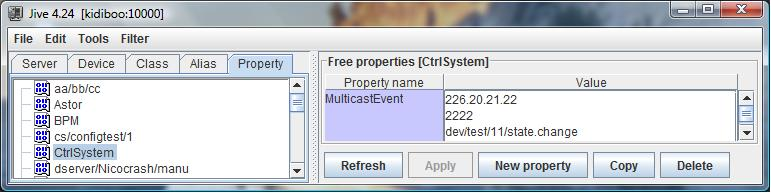
\includegraphics[scale=0.7]{advanced/jive_simpl}\end{center}

In the above window dump of the Jive tool, the \emph{change} event
on the \emph{state} attribute of the \emph{dev/test/11} device has
to be transferred using multicasting with the address \emph{226.20.21.22}
and the port number \emph{2222}. The exact definition of this CtrlSystem/MulticastEvent
property for one event propagated using multicast is

%
% Copyright (C) :      2004,2005,2006,2007,2008,2009,2010,2011,2012,2013
%                      European Synchrotron Radiation Facility
%                      BP 220, Grenoble 38043
%                      FRANCE
%
% This file is part of Tango.
%
% Tango is free software: you can redistribute it and/or modify
% it under the terms of the GNU Lesser General Public License as published by
% the Free Software Foundation, either version 3 of the License, or
% (at your option) any later version.
%
% Tango is distributed in the hope that it will be useful,
% but WITHOUT ANY WARRANTY; without even the implied warranty of
% MERCHANTABILITY or FITNESS FOR A PARTICULAR PURPOSE.  See the
% GNU Lesser General Public License for more details.
%
% You should have received a copy of the GNU Lesser General Public License
% along with Tango.  If not, see <http://www.gnu.org/licenses/>.
%
\begin{flushleft}
\begin{picture}(0,0)
\thicklines
\put(0,0){\line(1,0){400}}
\end{picture}
\end{flushleft}

\begin{lyxcode}
1~CtrlSystem->MulticastEvent:~~~Multicast~address,

2~~~~~~~~~~~~~~~~~~~~~~~~~~~~~~~port~number,

3~~~~~~~~~~~~~~~~~~~~~~~~~~~~~~~{[}rate~in~Mbit/sec{]},

4~~~~~~~~~~~~~~~~~~~~~~~~~~~~~~~{[}ivl~in~seconds{]},

5~~~~~~~~~~~~~~~~~~~~~~~~~~~~~~~event~name
\end{lyxcode}
%
% Copyright (C) :      2004,2005,2006,2007,2008,2009,2010,2011,2012,2013
%                      European Synchrotron Radiation Facility
%                      BP 220, Grenoble 38043
%                      FRANCE
%
% This file is part of Tango.
%
% Tango is free software: you can redistribute it and/or modify
% it under the terms of the GNU Lesser General Public License as published by
% the Free Software Foundation, either version 3 of the License, or
% (at your option) any later version.
%
% Tango is distributed in the hope that it will be useful,
% but WITHOUT ANY WARRANTY; without even the implied warranty of
% MERCHANTABILITY or FITNESS FOR A PARTICULAR PURPOSE.  See the
% GNU Lesser General Public License for more details.
%
% You should have received a copy of the GNU Lesser General Public License
% along with Tango.  If not, see <http://www.gnu.org/licenses/>.
%
\begin{flushleft}
\begin{picture}(0,0)
\thicklines
\put(0,0){\line(1,0){400}}
\end{picture}
\end{flushleft}


Rate\index{rate} and Ivl\index{ivl} are optional properties. In
case several events have to be transferred using multicasting, simply
extend the MulicastEvent property with the configuration parameters
related to the other events. There is only one MultiCastEvent property
per Tango control system. The underlying multicast protocol (PGM)
is rate limited. This means that it limits its network bandwidth usage
to a user defined value. The optional third configuration parameter
is the maximum rate (in Mbit/sec) that the protocol will use to transfert
this event. Because PGM is a reliable protocol, data has to be buffered
for re-transmission in case a receiver signal some lost data. The
optional forth configuration parameter specify the maximum amount
of time (in seconds) that a receiver can be absent for a multicast
group before unrecoverable data loss will occur. Exercise care when
setting large recovery interval as the data needed for recovery will
be held in memory. For example, a 60 seconds (1 minute) recovery interval
at a data rate of 1 Gbit/sec requires a 7 GBytes in-memory buffer.
Whan any of these two optional parameters are not set, the default
value (defined in next sub-chapter) are used. Here is another example
of events using multicasting configuration\begin{center}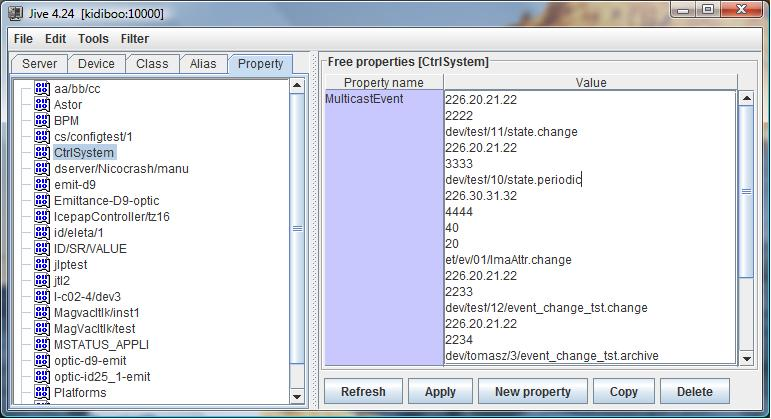
\includegraphics[scale=0.7]{advanced/jive_sophis}\end{center}
In this example, there are 5 events which are transmitted using multicasting:
\begin{enumerate}
\item Event \emph{change} for attribute \emph{state} on device \emph{dev/test/11}
which uses multicasting address \emph{226.20.21.22} and port number
\emph{2222}
\item Event \emph{periodic} for attribute \emph{state} on device \emph{dev/test/10}
which uses multicasting address \emph{226.20.21.22} and port number
\emph{3333}
\item Event \emph{change} for attribute \emph{ImaAttr} on device \emph{et/ev/01}
which uses multicasting address \emph{226.30.31.32} and port number
\emph{4444}. Note that this event uses a rate set to \emph{40 Mbit/sec}
and a ivl set to \emph{20 seconds}.
\item Event \emph{change} for attribute \emph{event\_change\_tst} on device
\emph{dev/test/12} which uses multicasting address \emph{226.20.21.22}
and port number \emph{2233}
\item Event \emph{archive} for attribute \emph{event\_change\_tst} on device
\emph{dev/tomasz/3} which uses multicasting address \emph{226.20.21.22}
and port number \emph{2234}
\end{enumerate}

\subsection{Default multicast related properties}

On top of the MulticastEvent property previously described, Tango
supports three properties to defined default value for multicast transport
tuning. These properties are:
\begin{itemize}
\item \textbf{MulticastRate}\index{MulticastRate} associated to the CtrlSystem\index{CtrlSystem}
object. This defines the maximum rate will will be used by the multicast
protocol when transferring event. The unit is Mbit/sec. In case this
property is not defined, the Tango library used a value of 80 Mbit/sec.
\item \textbf{MulticastIvl}\index{MulticastIvl} associated to the CtrlSystem
object. It specifies the maximum time (in sec) during which data has
to be buffered for re-transmission in case a receiver signals some
lost data. The unit is seconds. In case this property is not defined,
the Tango library takes a value of 20 seconds.
\item \textbf{MulticastHops}\index{MulticastHops} associated to the CtrlSystem
object. This property defines the maximum number of element (router),
the multicast packet is able to cross. Each time one element is crossed,
the value is decremented. When it reaches 0, the packet is not transferred
any more. In case this property is not defined, the Tango library
uses a value of 5.
\end{itemize}

\section{Memorized attribute}

It is possible to ask Tango to store in its database the last written
value for attribute of the SCALAR data format and obviously only for
READ\_WRITE or READ\_WITH\_WRITE attribute. This is fully automatic.
During device startup phase, for all device memorized\index{memorized}
attributes, the value written in the database is fetched and applied.
A write\_attribute call can be generated to apply the memorized value
to the attribute or only the attribute set point can be initialised.
The following piece of code shows how the source code should be written
to set an attribute as memorized and to initialise only the attribute
set point.

%
% Copyright (C) :      2004,2005,2006,2007,2008,2009,2010,2011,2012,2013
%                      European Synchrotron Radiation Facility
%                      BP 220, Grenoble 38043
%                      FRANCE
%
% This file is part of Tango.
%
% Tango is free software: you can redistribute it and/or modify
% it under the terms of the GNU Lesser General Public License as published by
% the Free Software Foundation, either version 3 of the License, or
% (at your option) any later version.
%
% Tango is distributed in the hope that it will be useful,
% but WITHOUT ANY WARRANTY; without even the implied warranty of
% MERCHANTABILITY or FITNESS FOR A PARTICULAR PURPOSE.  See the
% GNU Lesser General Public License for more details.
%
% You should have received a copy of the GNU Lesser General Public License
% along with Tango.  If not, see <http://www.gnu.org/licenses/>.
%
\begin{flushleft}
\begin{picture}(0,0)
\thicklines
\put(0,0){\line(1,0){400}}
\end{picture}
\end{flushleft}

\begin{lyxcode}
1~void~DevTestClass::attribute\_factory(vector<Tango::Attr~{*}>~\&att\_list)

2~~\{

3~~~~~~...

4~~~~~~att\_list.push\_back(new~String\_attrAttr());

5~~~~~~att\_list.back()->set\_memorized();

6~~~~~~att\_list.back()->set\_memorized\_init(false);

7~~~~~~...

8~~\}
\end{lyxcode}
%
% Copyright (C) :      2004,2005,2006,2007,2008,2009,2010,2011,2012,2013
%                      European Synchrotron Radiation Facility
%                      BP 220, Grenoble 38043
%                      FRANCE
%
% This file is part of Tango.
%
% Tango is free software: you can redistribute it and/or modify
% it under the terms of the GNU Lesser General Public License as published by
% the Free Software Foundation, either version 3 of the License, or
% (at your option) any later version.
%
% Tango is distributed in the hope that it will be useful,
% but WITHOUT ANY WARRANTY; without even the implied warranty of
% MERCHANTABILITY or FITNESS FOR A PARTICULAR PURPOSE.  See the
% GNU Lesser General Public License for more details.
%
% You should have received a copy of the GNU Lesser General Public License
% along with Tango.  If not, see <http://www.gnu.org/licenses/>.
%
\begin{flushleft}
\begin{picture}(0,0)
\thicklines
\put(0,0){\line(1,0){400}}
\end{picture}
\end{flushleft}


Line 4 : The attribute to be memorized is created and inserted in
the attribute vector.

Line 5 : The \emph{set\_memorized()} method of the attribute base
class is called to define the attribute as memorized.

Line 6 : The set\_memorized\_init() method is called with the parameter
false to define that only the set point should be initialsied.


\section{Forwarded attribute}


\subsection{Definition}

Let's take an example to explain what is a forwarded attribute. We
assume we have to write a Tango class for a ski lift in a ski resort
somewhere in the Alps. Obviously, the ski lift has a motor for which
we already have a Tango class. This motor Tango class has one attribute
\emph{speed}. But for the ski lift, the motor speed is not the only
thing which has to be controlled. For instance, you also want to give
access to the wind sensor data installed on the top of the ski lift.
Therefore, you write a ski-lift Tango class representing the whole
ski-lift system. This ski-lift class will have at least two attributes
which are:
\begin{enumerate}
\item The wind speed at the top of the ski-lift
\item The motor speed
\end{enumerate}
The ski-lift Tango class motor speed attribute is nothing more than
the motor Tango class speed attribute. All the ski-lift class has
to do for this attribute is to forward the request (read/write) to
the speed attribute of the motor Tango class. The speed attribute
of the ski-lift Tango class is a \textbf{forwarded attribute\index{forwarded-attribute}}
while the speed attribute of the motor Tango class is its \textbf{root
attribute}\index{root-attribute}.

A forwarded attribute get its configuration from its root attribute
and it forwards to its root attribute
\begin{itemize}
\item Its read / write / write\_read requests
\item Its configuration change
\item Its event subscription
\item Its locking behavior
\end{itemize}
As stated above, a forwarded attribute has the same configuration
than its root attribute except its \emph{name} and \emph{label} which
stays local. All other attribute configuration parameters are forwarded
to the root attribute. If a root attribute configuration parameter
is changed, the forwarded attribute is informed (via event) and its
local configuration is also modified.

The association between the forwarded attribute and its root attribute
is done using a property named \begin{center}\_\_root\_att\end{center}
belonging to the forwarded attribute. This property value is simply
the name of the root attribute. Muti-control system is supported and
this \_\_root\_att\index{__root_att@\_\_root\_att} attribute property
value can be something like \emph{tango://my\_tango\_host:10000/my/favorite/dev/the\_root\_attribute}.
The name of the root attribute is included in attribute configuration.

It is forbidden to poll a forwarded attribute and one exception is
thrown if such a case happens. Polling has to be done on the root
attribute. Nevertheless, if the root attribute is polled, a request
to read the forwarded attribute with the DeviceProxy object source
parameter set to CACHE\_DEVICE or CACHE will get its data from the
root attribute polling buffer.

If you subscribe to event(s) on a forwarded attribute, the subscription
is forwarded to the root attribute. When the event is received by
the forwarded attribute, the attribute name in the event data is modified
to reflect the forwarded attribute name and the event is pushed to
the original client(s).

When a device with forwarded attribute is locked, the device to which
the root attribute belongs is also locked.


\subsection{Coding}

As explained in the chapter \textquotedbl{}Writing a Tango device
server\textquotedbl{}, each Tango class attribute is implemented via
a C++ class which has to inherit from either \emph{Attr}, \emph{SpectrumAttr}
or \emph{ImageAttr} according to the attribute data format. For forwarded
attribute, the related class has to inherit from the \textbf{FwdAttr\index{FwdAttr}}
class whatever its data format is. For classical attribute, the programmer
can define in the Tango class code default value for the attribute
properties using one instance of the \emph{UserDefaultAttrProp} class.
For forwarded attribute, the programmer has to create one instance
of the \textbf{UserDefaultFwdAttrProp\index{UserDefaultFwdAttrProp}}
class but only the attribute label can be defined. One example of
how to program a forwarded attribute is given below

%
% Copyright (C) :      2004,2005,2006,2007,2008,2009,2010,2011,2012,2013
%                      European Synchrotron Radiation Facility
%                      BP 220, Grenoble 38043
%                      FRANCE
%
% This file is part of Tango.
%
% Tango is free software: you can redistribute it and/or modify
% it under the terms of the GNU Lesser General Public License as published by
% the Free Software Foundation, either version 3 of the License, or
% (at your option) any later version.
%
% Tango is distributed in the hope that it will be useful,
% but WITHOUT ANY WARRANTY; without even the implied warranty of
% MERCHANTABILITY or FITNESS FOR A PARTICULAR PURPOSE.  See the
% GNU Lesser General Public License for more details.
%
% You should have received a copy of the GNU Lesser General Public License
% along with Tango.  If not, see <http://www.gnu.org/licenses/>.
%
\begin{flushleft}
\begin{picture}(0,0)
\thicklines
\put(0,0){\line(1,0){400}}
\end{picture}
\end{flushleft}

\begin{lyxcode}
1~~class~MyFwdAttr:~public~Tango::FwdAttr

2~~\{~

3~~public:~~~~~

4~~~~~~MyFwdAttr(const~string~\&\_n):FwdAttr(\_n)~\{\};~	

5~~~~~~\textasciitilde{}MyFwdAttr()~\{\};~

6~~\};

7

8~~void~DevTestClass::attribute\_factory(vector<Tango::Attr~{*}>~\&att\_list)

9~~\{

10~~~~~...

11~~~~~MyFwdAttr~{*}att1~=~new~MyFwdAttr(\textquotedbl{}fwd\_att\_name\textquotedbl{});

12~~~~~Tango::UserDefaultFwdAttrProp~att1\_prop;~	

13~~~~~att1\_prop.set\_label(\textquotedbl{}Gasp~a~fwd~attribute\textquotedbl{});

14~~~~~att1->set\_default\_properties(att1\_prop);~	

15~~~~~att\_list.push\_back(att1);

14~~~~~...

15~~\}
\end{lyxcode}
%
% Copyright (C) :      2004,2005,2006,2007,2008,2009,2010,2011,2012,2013
%                      European Synchrotron Radiation Facility
%                      BP 220, Grenoble 38043
%                      FRANCE
%
% This file is part of Tango.
%
% Tango is free software: you can redistribute it and/or modify
% it under the terms of the GNU Lesser General Public License as published by
% the Free Software Foundation, either version 3 of the License, or
% (at your option) any later version.
%
% Tango is distributed in the hope that it will be useful,
% but WITHOUT ANY WARRANTY; without even the implied warranty of
% MERCHANTABILITY or FITNESS FOR A PARTICULAR PURPOSE.  See the
% GNU Lesser General Public License for more details.
%
% You should have received a copy of the GNU Lesser General Public License
% along with Tango.  If not, see <http://www.gnu.org/licenses/>.
%
\begin{flushleft}
\begin{picture}(0,0)
\thicklines
\put(0,0){\line(1,0){400}}
\end{picture}
\end{flushleft}


Line 1 : The forwarded attribute class inherits from FwdAttr class.

Line 4-5 : Only constructor and destructor methods are required

Line 11 : The attribute object is created

Line 12-14 : A default value for the forwarded attribute label is
defined.

Line 15: The forwarded attribute is added to the list of attribute

In case of error in the forwarded attribute configuration (for instance
missing \_\_root\_att property), the attribute is not created by the
Tango kernel and is therefore not visible for the external world.
The state of the device to which the forwarded attribute belongs to
is set to ALARM (if not already FAULT) and a detailed error report
is available in the device status. In case a device with forwarded
attribute(s) is started before the device(s) with the root attribute(s),
the same principle is used: forwarded attribute(s) are not created,
device state is set to ALARM and device status is reporting the error.
When the device(s) with the root attribute will start, the forwarded
attributes will automatically be created. 


\section{Transferring images}

Some optimized methods have been written to optimize image transfer
between client and server using the attribute DevEncoded\index{DevEncoded}
data type. All these methods have been merged in a class called EncodedAttribute.
Within this class, you will find methods to:
\begin{itemize}
\item Encode an image in a compressed way (JPEG\index{JPEG}) for images
coded on 8 (gray scale), 24 or 32 bits
\item Encode a grey scale image coded on 8 or 16 bits
\item Encode a color image coded on 24 bits
\item Decode images coded on 8 or 16 bits (gray scale) and returned a 8
or 16 bits grey scale image
\item Decode color images transmitted using a compressed format (JPEG) and
returns a 32 bits RGB image
\end{itemize}
The following code snippets are examples of how these methods have
to be used in a server and in a client. On the server side, creates
an instance of the EncodedAttribute\index{EncodedAttribute} class
within your object

%
% Copyright (C) :      2004,2005,2006,2007,2008,2009,2010,2011,2012,2013
%                      European Synchrotron Radiation Facility
%                      BP 220, Grenoble 38043
%                      FRANCE
%
% This file is part of Tango.
%
% Tango is free software: you can redistribute it and/or modify
% it under the terms of the GNU Lesser General Public License as published by
% the Free Software Foundation, either version 3 of the License, or
% (at your option) any later version.
%
% Tango is distributed in the hope that it will be useful,
% but WITHOUT ANY WARRANTY; without even the implied warranty of
% MERCHANTABILITY or FITNESS FOR A PARTICULAR PURPOSE.  See the
% GNU Lesser General Public License for more details.
%
% You should have received a copy of the GNU Lesser General Public License
% along with Tango.  If not, see <http://www.gnu.org/licenses/>.
%
\begin{flushleft}
\begin{picture}(0,0)
\thicklines
\put(0,0){\line(1,0){400}}
\end{picture}
\end{flushleft}

\begin{lyxcode}
1~class~MyDevice::Tango::Device\_4Impl

2~~\{

3~~~~~~...

4~~~~~~Tango::EncodedAttribute~jpeg;

5~~~~~~...

6~~\}
\end{lyxcode}
%
% Copyright (C) :      2004,2005,2006,2007,2008,2009,2010,2011,2012,2013
%                      European Synchrotron Radiation Facility
%                      BP 220, Grenoble 38043
%                      FRANCE
%
% This file is part of Tango.
%
% Tango is free software: you can redistribute it and/or modify
% it under the terms of the GNU Lesser General Public License as published by
% the Free Software Foundation, either version 3 of the License, or
% (at your option) any later version.
%
% Tango is distributed in the hope that it will be useful,
% but WITHOUT ANY WARRANTY; without even the implied warranty of
% MERCHANTABILITY or FITNESS FOR A PARTICULAR PURPOSE.  See the
% GNU Lesser General Public License for more details.
%
% You should have received a copy of the GNU Lesser General Public License
% along with Tango.  If not, see <http://www.gnu.org/licenses/>.
%
\begin{flushleft}
\begin{picture}(0,0)
\thicklines
\put(0,0){\line(1,0){400}}
\end{picture}
\end{flushleft}


In the code of your device, use an encoding method of the EncodedAttribute
class

%
% Copyright (C) :      2004,2005,2006,2007,2008,2009,2010,2011,2012,2013
%                      European Synchrotron Radiation Facility
%                      BP 220, Grenoble 38043
%                      FRANCE
%
% This file is part of Tango.
%
% Tango is free software: you can redistribute it and/or modify
% it under the terms of the GNU Lesser General Public License as published by
% the Free Software Foundation, either version 3 of the License, or
% (at your option) any later version.
%
% Tango is distributed in the hope that it will be useful,
% but WITHOUT ANY WARRANTY; without even the implied warranty of
% MERCHANTABILITY or FITNESS FOR A PARTICULAR PURPOSE.  See the
% GNU Lesser General Public License for more details.
%
% You should have received a copy of the GNU Lesser General Public License
% along with Tango.  If not, see <http://www.gnu.org/licenses/>.
%
\begin{flushleft}
\begin{picture}(0,0)
\thicklines
\put(0,0){\line(1,0){400}}
\end{picture}
\end{flushleft}

\begin{lyxcode}
1~void~MyDevice::read\_Encoded\_attr\_image(Tango::Attribute~\&att)

2~\{

3~~~~~~....

4~~~~~~jpeg.encode\_jpeg\_gray8(imageData,256,256,50.0);

5~~~~~~att.set\_value(\&jpeg);

6~\}
\end{lyxcode}
%
% Copyright (C) :      2004,2005,2006,2007,2008,2009,2010,2011,2012,2013
%                      European Synchrotron Radiation Facility
%                      BP 220, Grenoble 38043
%                      FRANCE
%
% This file is part of Tango.
%
% Tango is free software: you can redistribute it and/or modify
% it under the terms of the GNU Lesser General Public License as published by
% the Free Software Foundation, either version 3 of the License, or
% (at your option) any later version.
%
% Tango is distributed in the hope that it will be useful,
% but WITHOUT ANY WARRANTY; without even the implied warranty of
% MERCHANTABILITY or FITNESS FOR A PARTICULAR PURPOSE.  See the
% GNU Lesser General Public License for more details.
%
% You should have received a copy of the GNU Lesser General Public License
% along with Tango.  If not, see <http://www.gnu.org/licenses/>.
%
\begin{flushleft}
\begin{picture}(0,0)
\thicklines
\put(0,0){\line(1,0){400}}
\end{picture}
\end{flushleft}


Line 4: Image encoding. The size of the image is 256 by 256. Each
pixel is coded using 8 bits. The encoding quality is defined to 50
in a scale of 0 - 100. imageData is the pointer to the image data
(pointer to unsigned char)

Line 5: Set the value of the attribute using a \emph{Attribute::set\_value()}
method.

On the client side, the code is the following (without exception management)

%
% Copyright (C) :      2004,2005,2006,2007,2008,2009,2010,2011,2012,2013
%                      European Synchrotron Radiation Facility
%                      BP 220, Grenoble 38043
%                      FRANCE
%
% This file is part of Tango.
%
% Tango is free software: you can redistribute it and/or modify
% it under the terms of the GNU Lesser General Public License as published by
% the Free Software Foundation, either version 3 of the License, or
% (at your option) any later version.
%
% Tango is distributed in the hope that it will be useful,
% but WITHOUT ANY WARRANTY; without even the implied warranty of
% MERCHANTABILITY or FITNESS FOR A PARTICULAR PURPOSE.  See the
% GNU Lesser General Public License for more details.
%
% You should have received a copy of the GNU Lesser General Public License
% along with Tango.  If not, see <http://www.gnu.org/licenses/>.
%
\begin{flushleft}
\begin{picture}(0,0)
\thicklines
\put(0,0){\line(1,0){400}}
\end{picture}
\end{flushleft}

\begin{lyxcode}
1~~~~....

2~~~~DeviceAttribute~da;

3~~~~EncodedAttribute~att;

4~~~~int~width,height;

5~~~~unsigned~char~{*}gray8;

6~~~~~~

7~~~~da~=~device.read\_attribute(\textquotedbl{}Encoded\_attr\_image\textquotedbl{});

8~~~~att.decode\_gray8(\&da,\&width,\&height,\&gray8);

9~~~~....

10~~~delete~{[}{]}~gray8;

11~~~...
\end{lyxcode}
%
% Copyright (C) :      2004,2005,2006,2007,2008,2009,2010,2011,2012,2013
%                      European Synchrotron Radiation Facility
%                      BP 220, Grenoble 38043
%                      FRANCE
%
% This file is part of Tango.
%
% Tango is free software: you can redistribute it and/or modify
% it under the terms of the GNU Lesser General Public License as published by
% the Free Software Foundation, either version 3 of the License, or
% (at your option) any later version.
%
% Tango is distributed in the hope that it will be useful,
% but WITHOUT ANY WARRANTY; without even the implied warranty of
% MERCHANTABILITY or FITNESS FOR A PARTICULAR PURPOSE.  See the
% GNU Lesser General Public License for more details.
%
% You should have received a copy of the GNU Lesser General Public License
% along with Tango.  If not, see <http://www.gnu.org/licenses/>.
%
\begin{flushleft}
\begin{picture}(0,0)
\thicklines
\put(0,0){\line(1,0){400}}
\end{picture}
\end{flushleft}


The attribute named Encoded\_attr\_image is read at line7. The image
is decoded at line 8 in a 8 bits gray scale format. The image data
are stored in the buffer pointed to by \textquotedbl{}gray8\textquotedbl{}.
The memory allocated by the image decoding at line 8 is returned to
the system at line 10.


\section{Device server with user defined event loop}

Sometimes, it could be usefull to write your own process event handling
loop\index{event-loop}. For instance, this feature can be used in
a device server process where the ORB is only one of several components
that must perform event handling. A device server with a graphical
user interface must allow the GUI to handle windowing events in addition
to allowing the ORB to handle incoming requests. These types of device
server therefore perform non-blocking event handling. They turn the
main thread of control over each of the vvarious event-handling sub-systems
while not allowing any of them to block for significants period of
time. The \emph{Tango::Util} class has a method called \emph{server\_set\_event\_loop()\index{server-set-event-loop}}
to deal with such a case. This method has only one argument which
is a function pointer. This function does not receive any argument
and returns a boolean. If this boolean is true, the device server
process exits. The device server core will call this function in a
loop without any sleeping time between the call. It is the user responsability
to implement in this function some kind of sleeping mechanism in order
not to make this loop too CPU consuming. The code of this function
is executed by the device server main thread\index{thread}. The following
piece of code is an example of how you can use this feature.

%
% Copyright (C) :      2004,2005,2006,2007,2008,2009,2010,2011,2012,2013
%                      European Synchrotron Radiation Facility
%                      BP 220, Grenoble 38043
%                      FRANCE
%
% This file is part of Tango.
%
% Tango is free software: you can redistribute it and/or modify
% it under the terms of the GNU Lesser General Public License as published by
% the Free Software Foundation, either version 3 of the License, or
% (at your option) any later version.
%
% Tango is distributed in the hope that it will be useful,
% but WITHOUT ANY WARRANTY; without even the implied warranty of
% MERCHANTABILITY or FITNESS FOR A PARTICULAR PURPOSE.  See the
% GNU Lesser General Public License for more details.
%
% You should have received a copy of the GNU Lesser General Public License
% along with Tango.  If not, see <http://www.gnu.org/licenses/>.
%
\begin{flushleft}
\begin{picture}(0,0)
\thicklines
\put(0,0){\line(1,0){400}}
\end{picture}
\end{flushleft}

\begin{lyxcode}
~~~~~1~~

~~~~~2~~bool~my\_event\_loop()

~~~~~3~~\{

~~~~~4~~~~~bool~ret;

~~~~~5~~

~~~~~6~~~~~some\_sleeping\_time();

~~~~~7~~

~~~~~8~~~~~ret~=~handle\_gui\_events();

~~~~~9~~

~~~~10~~~~~return~ret;

~~~~11~~\}

~~~~12~~

~~~~13~~int~main(int~argc,char~{*}argv{[}{]})

~~~~14~~\{

~~~~15~~~~~Tango::Util~{*}tg;

~~~~16~~~~~try

~~~~17~~~~~\{

~~~~18~~~~~~~~//~Initialise~the~device~server

~~~~19~~~~~~~~//-{}-{}-{}-{}-{}-{}-{}-{}-{}-{}-{}-{}-{}-{}-{}-{}-{}-{}-{}-{}-{}-{}-{}-{}-{}-{}-{}-{}-{}-{}-{}-{}-{}-{}-{}-{}-{}-{}-{}-

~~~~20~~~~~~~~tg~=~Tango::Util::init(argc,argv);

~~~~21~~

~~~~22~~~~~~~~tg->set\_polling\_threads\_pool\_size(5);

~~~~23~~

~~~~24~~~~~~~~//~Create~the~device~server~singleton~

~~~~25~~~~~~~~//~~~~~~~~which~will~create~everything

~~~~26~~~~~~~~//-{}-{}-{}-{}-{}-{}-{}-{}-{}-{}-{}-{}-{}-{}-{}-{}-{}-{}-{}-{}-{}-{}-{}-{}-{}-{}-{}-{}-{}-{}-{}-{}-{}-{}-{}-{}-{}-{}-{}-

~~~~27~~~~~~~~tg->server\_init(false);

~~~~28~~

~~~~29~~~~~~~~tg->server\_set\_event\_loop(my\_event\_loop);

~~~~30~~

~~~~31~~~~~~~~//~Run~the~endless~loop

~~~~32~~~~~~~~//-{}-{}-{}-{}-{}-{}-{}-{}-{}-{}-{}-{}-{}-{}-{}-{}-{}-{}-{}-{}-{}-{}-{}-{}-{}-{}-{}-{}-{}-{}-{}-{}-{}-{}-{}-{}-{}-{}-{}-

~~~~33~~~~~~~~cout~<\textcompwordmark{}<~\textquotedbl{}Ready~to~accept~request\textquotedbl{}~<\textcompwordmark{}<~endl;

~~~~34~~~~~~~~tg->server\_run();

~~~~35~~~~~\}

~~~~36~~~~~catch~(bad\_alloc)

~~~~37~~~~~\{

~~~~38~~~~~...
\end{lyxcode}
%
% Copyright (C) :      2004,2005,2006,2007,2008,2009,2010,2011,2012,2013
%                      European Synchrotron Radiation Facility
%                      BP 220, Grenoble 38043
%                      FRANCE
%
% This file is part of Tango.
%
% Tango is free software: you can redistribute it and/or modify
% it under the terms of the GNU Lesser General Public License as published by
% the Free Software Foundation, either version 3 of the License, or
% (at your option) any later version.
%
% Tango is distributed in the hope that it will be useful,
% but WITHOUT ANY WARRANTY; without even the implied warranty of
% MERCHANTABILITY or FITNESS FOR A PARTICULAR PURPOSE.  See the
% GNU Lesser General Public License for more details.
%
% You should have received a copy of the GNU Lesser General Public License
% along with Tango.  If not, see <http://www.gnu.org/licenses/>.
%
\begin{flushleft}
\begin{picture}(0,0)
\thicklines
\put(0,0){\line(1,0){400}}
\end{picture}
\end{flushleft}


The device server main event loop is set at line 29 before the call
to the Util::server\_run() method. The function used as server loop
is defined between lines 2 and 11.


\section{Device server using file\index{file} as database\index{database}\label{sec:Device-server-file}}

For device servers not able to access the Tango database (most of
the time due to network route or security reason), it is possible
to start them using file instead of a real database. This is done
via the device server\begin{center}-file=<file name>\end{center}
command line option. In this case,
\begin{itemize}
\item Getting, setting and deleting class properties
\item Getting, setting and deleting device properties
\item Getting, setting and deleting class attribute properties
\item Getting, setting and deleting device attribute properties
\end{itemize}
are handled using the specified file instead of the Tango database.
The file is an ASCII file and follows a well-defined syntax with predefined
keywords. The simplest way to generate the file for a specific device
server is to use the Jive application. See  \cite{Jive doc} to get
Jive documentation. The Tango database is not only used to store device
configuration parameters, it is also used to store device network
access parameter (the CORBA IOR). To allow an application to connect
to a device hosted by a device server using file instead of database,
you need to start it on a pre-defined port\index{port}, and you must
use one of the underlying ORB option called \emph{endPoint} like \begin{center}myserver
myinstance\_name -file=/tmp/MyServerFile -ORBendPoint giop:tcp::<port
number>\end{center} to start your device server. The device name
passed to the client application must also be modified in order to
refect the non-database usage. See \ref{DeviceNaming} to learn about
Tango device name syntax. Nevertheless, using this Tango feature prevents
some other features to be used :
\begin{itemize}
\item No check that the same device server is running twice.
\item No device or attribute alias name.
\item In case of several device servers running on the same host, the user
must manually manage a list of already used network port.
\end{itemize}

\section{Device server without database\label{sec:Device-server-without}}

In some very specific cases (Running a device server within a lab
during hardware development...), it could be very useful to have a
device server able to run even if there is no database\index{database}
in the control system. Obviously, running a Tango device server without
a database means loosing Tango features. The lost features are :
\begin{itemize}
\item No check that the same device server is running twice.
\item No device configuration via properties.
\item No event generated by the server.
\item No memorized attributes
\item No device attribute configuration via the database.
\item No check that the same device name is used twice within the same control
system.
\item In case of several device servers running on the same host, the user
must manually manage a list of already used network port.
\end{itemize}
To run a device server without a database, the \textbf{-nodb\index{nodb}}
command line option must be used. One problem when running a device
server without the database is to pass device name(s) to the device
server. Within Tango, it is possible to define these device names
at two different levels :
\begin{enumerate}
\item At the command line with the \textbf{-dlist\index{dlist}} option:
In case of device server with several device pattern implementation,
the device name list given at command line is only for the last device
pattern created in the \emph{class\_factory()} method. In the device
name list, the device name separator is the comma character.
\item At the device pattern implementation level: In the class inherited
from the Tango::DeviceClass class via the re-definition of a well
defined method called \emph{device\_name\_factory()}
\end{enumerate}
If none of these two possibilities is used, the tango core classes
defined one default device name for each device pattern implementation.
This default device name is \emph{NoName}. Device definition at the
command line has the highest priority.


\subsection{Example of device server started without database usage}

Without database, you need to start a Tango device server on a pre-defined
port\index{port}, and you must use one of the underlying ORB option
called \emph{endPoint} like \begin{center}myserver myinstance\_name
-ORBendPoint giop:tcp::<port number> -nodb -dlist a/b/c\end{center}

The following is two examples of starting a device server not using
the database when the \emph{device\_name\_factory()} method is not
re-defined.
\begin{itemize}
\item StepperMotor et -nodb -dlist id11/motor/1,id11/motor/2\\
This command line starts the device server with two devices named
\emph{id11/motor/1} and \emph{id11/motor/2}
\item StepperMotor et -nodb\\
This command line starts a device server with one device named \emph{NoName}
\end{itemize}
When the \emph{device\_name\_factory()} method is re-defined within
the StepperMotorClass class.

%
% Copyright (C) :      2004,2005,2006,2007,2008,2009,2010,2011,2012,2013
%                      European Synchrotron Radiation Facility
%                      BP 220, Grenoble 38043
%                      FRANCE
%
% This file is part of Tango.
%
% Tango is free software: you can redistribute it and/or modify
% it under the terms of the GNU Lesser General Public License as published by
% the Free Software Foundation, either version 3 of the License, or
% (at your option) any later version.
%
% Tango is distributed in the hope that it will be useful,
% but WITHOUT ANY WARRANTY; without even the implied warranty of
% MERCHANTABILITY or FITNESS FOR A PARTICULAR PURPOSE.  See the
% GNU Lesser General Public License for more details.
%
% You should have received a copy of the GNU Lesser General Public License
% along with Tango.  If not, see <http://www.gnu.org/licenses/>.
%
\begin{flushleft}
\begin{picture}(0,0)
\thicklines
\put(0,0){\line(1,0){400}}
\end{picture}
\end{flushleft}

\begin{lyxcode}
~~~~~1~~void~StepperMotorClass::device\_name\_factory(vector<string>~\&list)

~~~~~2~~\{

~~~~~3~~~~~~list.push\_back(\textquotedbl{}sr/cav-tuner/1\textquotedbl{});

~~~~~4~~~~~~list.push\_back(\textquotedbl{}sr/cav-tuner/2\textquotedbl{});

~~~~~5~~\}
\end{lyxcode}
%
% Copyright (C) :      2004,2005,2006,2007,2008,2009,2010,2011,2012,2013
%                      European Synchrotron Radiation Facility
%                      BP 220, Grenoble 38043
%                      FRANCE
%
% This file is part of Tango.
%
% Tango is free software: you can redistribute it and/or modify
% it under the terms of the GNU Lesser General Public License as published by
% the Free Software Foundation, either version 3 of the License, or
% (at your option) any later version.
%
% Tango is distributed in the hope that it will be useful,
% but WITHOUT ANY WARRANTY; without even the implied warranty of
% MERCHANTABILITY or FITNESS FOR A PARTICULAR PURPOSE.  See the
% GNU Lesser General Public License for more details.
%
% You should have received a copy of the GNU Lesser General Public License
% along with Tango.  If not, see <http://www.gnu.org/licenses/>.
%
\begin{flushleft}
\begin{picture}(0,0)
\thicklines
\put(0,0){\line(1,0){400}}
\end{picture}
\end{flushleft}

\begin{itemize}
\item StepperMotor et -nodb\\
This commands starts a device server with two devices named \emph{sr/cav-tuner/1}
and \emph{sr/cav-tuner/2}.
\item StepperMotor et -nodb -dlist id12/motor/1\\
Starts a device server with only one device named id12/motor/1
\end{itemize}

\subsection{Connecting client to device within a device server started without
database}

In this case, the host and port on which the device server is running
are part of the device name. If the device name is \emph{a/b/c}, the
host is \emph{mycomputer} and the port \emph{1234}, the device name
to be used by client is\begin{center}mycomputer:1234/a/b/c\#dbase=no\end{center}

See appendix \ref{DeviceNaming} for all details about Tango object
naming.


\section{Multiple database servers within a Tango control system}

Tango uses MySQL as database and allows access to this database via
a specific Tango device server. It is possible for the same Tango
control system to have several Tango database servers. The host name
and port number of the database server is known via the TANGO\_HOST\index{TANGO-HOST}
environment variable. If you want to start several database servers
in order to prevent server crash, use the following TANGO\_HOST syntax\begin{center}

TANGO\_HOST=<host\_1>:<port\_1>,<host\_2>:<port\_2>,<host\_3>:<port\_3>\end{center}

All calls to the database server will automatically switch to a running
servers in the given list if the one used dies.


\section{The Tango controlled access system\index{controlled-access}}


\subsection{User rights definition}

Within the Tango controlled system, you give rights to a user. User
is the name of the user used to log-in the computer where the application
trying to access a device is running. Two kind of users are defined:
\begin{enumerate}
\item Users with defined rights
\item Users without any rights defined in the controlled system. These users
will have the rights associated with the pseudo-user called \textquotedbl{}All
Users\textquotedbl{}
\end{enumerate}
The controlled system manages two kind of rights:
\begin{itemize}
\item Write access meaning that all type of requests are allowed on the
device
\item Read access meaning that only read-like access are allowed (write\_attribute,
write\_read\_attribute and set\_attribute\_config network calls are
forbidden). Executing a command is also forbidden except for commands
defined as \textquotedbl{}\textbf{Allowed commands}\textquotedbl{}.
Getting a device state or status using the command\_inout call is
always allowed. The definition of the allowed commands is done at
the device class level. Therefore, all devices belonging to the same
class will have the allowed commands set.
\end{itemize}
The rights given to a user is the check result splitted in two levels:
\begin{enumerate}
\item At the host level: You define from which hosts the user may have write
access to the control system by specifying the host name. If the request
comes from a host which is not defined, the right will be Read access.
If nothing is defined at this level for the user, the rights of the
\textquotedbl{}All Users\textquotedbl{} user will be used. It is also
possible to specify the host by its IP address. You can define a host
family using wide-card in the IP address (eg. 160.103.11.{*} meaning
any host with IP address starting with 160.103.11). Only IP V4 is
supported. 
\item At the device level: You define on which device(s) request are allowed
using device name. Device family can be used using widecard in device
name like domin/family/{*}
\end{enumerate}
Therefore, the controlled system is doing the following checks when
a client try to access a device:
\begin{itemize}
\item Get the user name
\item Get the host IP address
\item If rights defined at host level for this specific user and this IP
address, gives user temporary write acccess to the control system
\item If nothing is specified for this specific user on this host, gives
to the user a temporary access right equal to the host access rights
of the \textquotedbl{}All User\textquotedbl{} user.
\item If the temporary right given to the user is write access to the control
system

\begin{itemize}
\item If something defined at device level for this specific user

\begin{itemize}
\item If there is a right defined for the device to be accessed (or for
the device family), give user the defined right
\item Else

\begin{itemize}
\item If rights defined for the \textquotedbl{}All Users\textquotedbl{}
user for this device, give this right to the user
\item Else, give user the Read Access for this device
\end{itemize}
\end{itemize}
\item Else

\begin{itemize}
\item If there is a right defined for the device to be accessed (or for
the device family) for the \textquotedbl{}All User\textquotedbl{}
user, give user this right
\item Else, give user the Read Access right for this device
\end{itemize}
\end{itemize}
\item Else, access right will be Read Access
\end{itemize}
Then, when the client tries to access the device, the following algorithm
is used:
\begin{itemize}
\item If right is Read Access

\begin{itemize}
\item If the call is a write type call, refuse the call
\item If the call is a command execution

\begin{itemize}
\item If the command is one of the command defined in the \textquotedbl{}Allowed
commands\textquotedbl{} for the device class, send the call
\item Else, refuse the call
\end{itemize}
\end{itemize}
\end{itemize}
All these checks are done during the DeviceProxy instance constructor
except those related to the device class allowed commands which are
checked during the command\_inout call.

To simplify the rights management, give the \textquotedbl{}All Users\textquotedbl{}
user host access right to all hosts (\textquotedbl{}{*}.{*}.{*}.{*}\textquotedbl{})
and read access to all devices (\textquotedbl{}{*}/{*}/{*}\textquotedbl{}).
With such a set-up for this user, each new user without any rights
defined in the controlled access will have only Read Access to all
devices on the control system but from any hosts. Then, on request,
gives Write Access to specific user on specific host (or family) and
on specific device (or family). 

The rights managements are done using the Tango Astor\cite{Astor_doc}
tool which has some graphical windows allowing to grant/revoke user
rights and to define device class allowed commands set. The following
window dump shows this Astor window.\begin{center}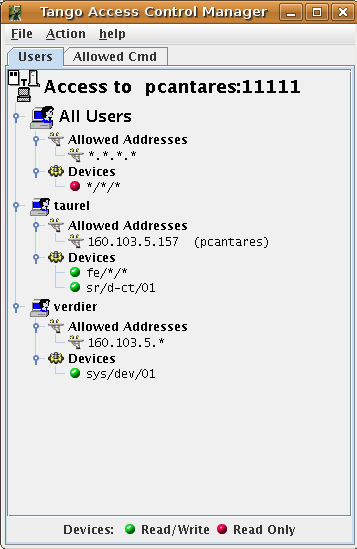
\includegraphics{advanced/control}\end{center}

In this example, the user \textquotedbl{}taurel\textquotedbl{} has
Write Access to the device \textquotedbl{}sr/d-ct/1\textquotedbl{}
and to all devices belonging to the domain \textquotedbl{}fe\textquotedbl{}
but only from the host \textquotedbl{}pcantares\textquotedbl{} He
has read access to all other devices but always only from the host
pcantares. The user \textquotedbl{}verdier\textquotedbl{} has write
access to the device \textquotedbl{}sys/dev/01\textquotedbl{} from
any host on the network \textquotedbl{}160.103.5\textquotedbl{} and
Read Access to all the remaining devices from the same network. All
the other users has only Read Access but from any host.


\subsection{Running a Tango control system with the controlled access}

All the users rights are stored in two tables of the Tango database.
A dedicated device server called \textbf{TangoAccessControl\index{TangoAccessControl}}
access these tables without using the classical Tango database server.
This TangoAccessControl device server must be configured with only
one device. The property \textbf{Services\index{Services} }belonging
to the free object\textbf{ CtrlSystem\index{CtrlSystem}} is used
to run a Tango control system with its controlled access. This property
is an array of string with each string describing the service(s) running
in the control system. For controlled access, the service name is
\textquotedbl{}AccessControl\textquotedbl{}. The service instance
name has to be defined as \textquotedbl{}tango\textquotedbl{}. The
device name associated with this service must be the name of the TangoAccessControl
server device. For instance, if the TangoAccessControl device server
device is named \emph{sys/access\_control/1}, one element of the Services
property of the CtrlSystem object has to be set to\begin{center}AccessControl/tango:sys/access\_control/1\end{center}

If the service is defined but without a valid device name corresponding
to the TangoAccessControl device server, all users from any host will
have write access (simulating a Tango control system without controlled
access). Note that this device server connects to the MySQL database
and therefore may need the MySQL connection related environment variables
MYSQL\_USER\index{MYSQL-USER} and MYSQL\_PASSWORD\index{MYSQL-PASSWORD}
described in \ref{sub:Db-Env-Variables}

Even if a controlled access system is running, it is possible to by-pass
it if, in the environment of the client application, the environment
variable SUPER\_TANGO\index{SUPER-TANGO} is defined to \textquotedbl{}true\textquotedbl{}.
If for one reason or another, the controlled access server is defined
but not accessible, the device right checked at that time will be
Read Access.\vspace{1cm}


\begin{center}
\label{FourRicardo}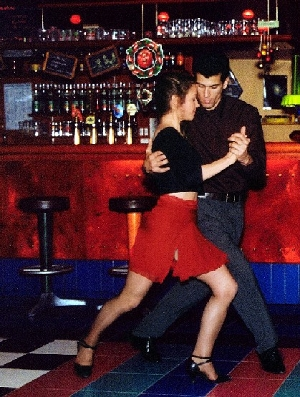
\includegraphics[scale=4]{dance/AT97-65-size}
\par\end{center}


\begin{comment}
The appendix 
\end{comment}

\appendix


\chapter{Reference part\label{cha:Reference-part}}

\textbf{This chapter is only part of the TANGO device server reference
guide. To get reference documentation about the C++ library classes,
see \cite{TANGO_ref_man}. To get reference documentation about the
Java classes, also see \cite{TANGO_ref_man}.}


\section{Device parameter}

A black box, a device description field, a device state and status
are associated with each TANGO device.


\subsection{The device black box}

The device black box\index{black-box} is managed as a circular buffer.
It is possible to tune the buffer depth via a device property. This
property name is \begin{center}device name->blackbox\_depth\end{center}
A default value is hard-coded to 50 if the property is not defined.
This black box depth property is retrieved from the Tango property
database during the device creation phase.


\subsection{The device description field}

There are two ways to intialise the device description\index{description}
field.
\begin{itemize}
\item At device creation time. Some constructors of the DeviceImpl class
supports this field as parameter. If these constructor are not used,
the device description field is set to a default value which is \emph{A
Tango device}.
\item With a property. A description field defines with this method overrides
a device description defined at construction time. The property name
is \begin{center}device name->description\end{center}
\end{itemize}

\subsection{The device state and status}

Some constructors of the DeviceImpl class allows the initialisation
of device state\index{state} and/or status\index{status} or device
creation time. If these fields are not defined, a default value is
applied. The default state is Tango::UNKOWN, the default status is
\emph{Not Initialised.}


\subsection{The device polling\label{sub:The-device-polling-prop}}

Seven device properties allow the polling tunning. These properties
are described in the following table 

\vspace{0.3cm}


\begin{center}
\begin{longtable}{|c|c|c|}
\hline 
Property name & property rule & default value\tabularnewline
\hline 
\hline 
poll\_ring\_depth & Polling buffer depth & 10\tabularnewline
\hline 
cmd\_poll\_ring\_depth & Cmd polling buffer depth & \tabularnewline
\hline 
attr\_poll\_ring\_depth & Attr polling buffer depth & \tabularnewline
\hline 
poll\_old\_factor & \textquotedbl{}Data too old\textquotedbl{} factor & 4\tabularnewline
\hline 
min\_poll\_period & Minimun polling period & \tabularnewline
\hline 
cmd\_min\_poll\_period & Min. polling period for cmd & \tabularnewline
\hline 
attr\_min\_poll\_period & Min. polling period for attr & \tabularnewline
\hline 
\end{longtable}
\par\end{center}

\vspace{0.3cm}


The rule of the poll\_ring\_depth\index{poll-ring-depth} property
is obvious. It defines the polling ring depth for all the device polled
command(s) and attribute(s). Nevertheless, when filling the polling
buffer via the fill\_cmd\_polling\_buffer()\index{fill-cmd-polling-buffer}
(or fill\_attr\_polling\_buffer()\index{fill-attr-polling-buffer})
method, it could be helpfull to define specific polling ring depth
for a command (or an attribute). This is the rule of the cmd\_poll\_ring\_depth\index{cmd-poll-ring-depth}
and attr\_poll\_ring\_depth\index{attr-poll-ring-depth} properties.
For each polled object with specific polling depth (command or attribute),
the syntax of this property is the object name followed by the ring
depth (ie State,20,Status,15). If one of these properties is defined,
for the specific command or attribute, it will overwrite the value
set by the poll\_ring\_depth property. The poll\_old\_factor\index{poll-old-factor}
property allows the user to tune how long the data recorded in the
polling buffer are valid. Each time some data are read from the polling
buffer, a check is done between the date when the data were recorded
in the polling buffer and the date when the user request these data.
If the interval is greater than the object polling period multiply
by the value of the poll\_old\_factor factory, an exception is returned
to the caller. These two properties are defined at device level and
therefore, it is not possible to tune this parameter for each polled
object (command or attribute). The last 3 properties are dedicated
to define a polling period minimum threshold. The property min\_poll\_period\index{min-poll-period}
defines in (mS) a device minimum polling period. Property cmd\_min\_poll\_period\index{cmd-min-poll-period}
defines (in mS) a minimum polling period for a specific command. The
syntax of this property is the command name followed by the minimum
polling period (ie MyCmd,400). Property attr\_min\_poll\_period\index{attr-min-poll-period}
defines (in mS) a minimum polling period for a specific attribute.
The syntax of this property is the attribute name followed by the
minimum polling period (ie MyAttr,600). These two properties has a
higher priority than the min\_poll\_period property. By default these
three properties are not defined mening that there is no minimun polling
period.

Four other properties are used by the Tango core classes to manage
the polling thread. These properties are :
\begin{itemize}
\item polled\_cmd to memorize the name of the device polled command
\item polled\_attr to memorize the name of the device polled attribute
\item non\_auto\_polled\_cmd to memorize the name of the command which shoule
not be polled automatically at the first request
\item non\_auto\_polled\_attr to memorize the name of the attribute which
should not be polled automatically at the first request
\end{itemize}
You don't have to change these properties values by yourself. They
are automatically created/modified/deleted by Tango core classes.


\subsection{The device logging}

The Tango Logging Service (TLS) uses device properties to control
device logging at startup (static configuration). These properties
are described in the following table 

\vspace{0.3cm}


\begin{center}
\begin{longtable}{|c|c|c|}
\hline 
Property name & property rule & default value\tabularnewline
\hline 
\hline 
logging\_level & Initial device logging level & WARN\tabularnewline
\hline 
logging\_target & Initial device logging target & No default\tabularnewline
\hline 
logging\_rft & Logging rolling file threshold & 20 Mega bytes\tabularnewline
\hline 
logging\_path & Logging file path & \multicolumn{1}{c|}{/tmp/tango-<logging name> or}\tabularnewline
 &  & C:/tango-<logging name> (Windows)\tabularnewline
\hline 
\end{longtable}
\par\end{center}

\vspace{0.3cm}

\begin{itemize}
\item The logging\_level\index{logging-level} property controls the initial
logging level of a device. Its set of possible values is: \textquotedbl{}OFF\textquotedbl{},
\textquotedbl{}FATAL\textquotedbl{}, \textquotedbl{}ERROR\textquotedbl{},
\textquotedbl{}WARN\textquotedbl{}, \textquotedbl{}INFO\textquotedbl{}
or \textquotedbl{}DEBUG\textquotedbl{}. This property is overwritten
by the verbose command line option (-v).
\item The logging\_target\index{logging-target} property is a multi-valued
property containing the initial target list. Each entry must have
the following format: target\_type::target\_name (where target\_type
is one of the supported target types and target\_name, the name of
the target). Supported target types are: \emph{console}, \emph{file}
and \emph{device}. For a device target, target\_name must contain
the name of a log consumer device (as defined in \ref{sec:Tango-log-consumer}).
For a file target, target\_name is the name of the file to log to.
If omitted the device's name is used to build the file name (domain\_family\_member.log).
Finally, target\_name is ignored in the case of a console target.
The TLS does not report any error occurred while trying to setup the
initial targets. 

\begin{itemize}
\item Logging\_target property example : \\
\\
logging\_target = {[} \textquotedbl{}console\textquotedbl{}, \textquotedbl{}file\textquotedbl{},
\textquotedbl{}file::/home/me/mydevice.log\textquotedbl{}, \textquotedbl{}device::tmp/log/1\textquotedbl{}{]}\\
\\
In this case, the device will automatically logs to the standard output,
to its default file (which is something like domain\_family\_member.log),
to a file named mydevice.log and located in /home/me. Finally, the
device logs are also sent to a log consumer device named tmp/log/1. 
\end{itemize}
\item The logging\_rft\index{logging-rft} property specifies the rolling
file threshold (rft), of the device's file targets. This threshold
is expressed in Kb. When the size of a log file reaches the so-called
rolling-file-threshold (rft), it is backuped as \textquotedbl{}\emph{current\_log\_file\_name}\textquotedbl{}
+ \textquotedbl{}\emph{\_1}\textquotedbl{} and a new current\_log\_file\_name
is opened. Obviously, there is only one backup file at a time (i.e.
any existing backup is destroyed before the current log file is backuped).
The default threshold is 20 Mb, the minimum is 500 Kb and the maximum
is 1000 Mb.
\item The logging\_path\index{logging-path} property overwrites the TANGO\_LOG\_PATH\index{TANGO-LOG-PATH}
environment variable. This property can only be applied to a DServer
class device and has no effect on other devices.
\end{itemize}

\section{Device attribute}

Attribute are configured with two kind of parameters: Parameters hard-coded
in source code and modifiable parameters


\subsection{Hard-coded device attribute parameters}

Seven attribute parameters are defined at attribute\index{attribute}
creation time in the Tango class source code. Obviously, these parameters
are not modifiable except with a new source code compilation. These
parameters are 

\vspace{0.3cm}


\begin{center}
\begin{longtable}{|c|c|}
\hline 
Parameter name & Parameter description\tabularnewline
\hline 
\hline 
name & Attribute name\tabularnewline
\hline 
data\_type & Attribute data type\tabularnewline
\hline 
data\_format & Attribute data format\tabularnewline
\hline 
writable\index{writable} & Attribute read/write type\tabularnewline
\hline 
max\_dim\_x & Maximum X dimension\tabularnewline
\hline 
max\_dim\_y & Maximum Y dimension\tabularnewline
\hline 
writable\_attr\_name\index{writable-attr-name} & Associated write attribute\tabularnewline
\hline 
level\index{level} & Attribute display level\tabularnewline
\hline 
root\_attr\_name & Root attribute name\tabularnewline
\hline 
\end{longtable}
\par\end{center}

\vspace{0.3cm}



\subsubsection{The Attribute data type\index{data-type}}

Thirteen data types are supported. These data types are
\begin{itemize}
\item Tango::DevBoolean 
\item Tango::DevShort
\item Tango::DevLong
\item Tango::DevLong64
\item Tango::DevFloat
\item Tango::DevDouble
\item Tango::DevUChar
\item Tango::DevUShort
\item Tango::DevULong
\item Tango::DevULong64
\item Tango::DevString
\item Tango::DevState
\item Tango::DevEncoded
\end{itemize}

\subsubsection{The attribute data format\index{data-format}}

Three data format are supported for attribute

\vspace{0.3cm}


\begin{center}
\begin{longtable}{|c|c|}
\hline 
Format & Description\tabularnewline
\hline 
\hline 
Tango::SCALAR\index{SCALAR} & The attribute value is a single number\tabularnewline
\hline 
Tango::SPECTRUM\index{SPECTRUM} & The attribute value is a one dimension number\tabularnewline
\hline 
Tango::IMAGE\index{IMAGE} & The attribute value is a two dimension number\tabularnewline
\hline 
\end{longtable}
\par\end{center}

\vspace{0.3cm}



\subsubsection{The max\_dim\_x\index{max-dim-x} and max\_dim\_y\index{max-dim-y}
parameters}

These two parameters defined the maximum size for attributes of the
SPECTRUM and IMAGE data format.

\vspace{0.3cm}


\begin{center}
\begin{longtable}{|c|c|c|}
\hline 
data format & max\_dim\_x & max\_dim\_y\tabularnewline
\hline 
\hline 
Tango::SCALAR & 1 & 0\tabularnewline
\hline 
Tango::SPECTRUM & User Defined & 0\tabularnewline
\hline 
Tango::IMAGE & User Defined & User Defined\tabularnewline
\hline 
\end{longtable}
\par\end{center}

\vspace{0.3cm}


For attribute of the Tango::IMAGE data format, all the data are also
returned in a one dimension array. The first array is value{[}0{]},{[}0{]},
array element X is value{[}0{]},{[}X-1{]}, array element X+1 is value{[}1{]}{[}0{]}
and so forth.


\subsubsection{The attribute read/write type}

Tango supports four kind of read/write attribute which are :
\begin{itemize}
\item Tango::READ\index{READ} for read only attribute
\item Tango::WRITE\index{WRITE} for writable attribute
\item Tango::READ\_WRITE\index{READ-WRITE} for attribute which can be read
and write
\item Tango::READ\_WITH\_WRITE\index{READ-WITH-WRITE} for a readable attribute
associated to a writable attribute (For a power supply device, the
current really generated is not the wanted current. To handle this,
two attributes are defined which are \emph{generated\_current} and
\emph{wanted\_current}. The \emph{wanted\_current} is a Tango::WRITE
attribute. When the \emph{generated\_current} attribute is read, it
is very convenient to also get the \emph{wanted\_current} attribute.
This is exactly what the Tango::READ\_WITH\_WRITE attribute is doing)
\end{itemize}
When read, attribute values are always returned within an array even
for scalar attribute. The length of this array and the meaning of
its elements is detailed in the following table for scalar attribute.

\vspace{0.3cm}


\begin{center}
\begin{longtable}{|c|c|c|c|}
\hline 
Name & Array length & Array{[}0{]} & Array{[}1{]}\tabularnewline
\hline 
\hline 
Tango::READ & 1 & Read value & \tabularnewline
\hline 
Tango::WRITE & 1 & Last write value & \tabularnewline
\hline 
Tango::READ\_WRITE & 2 & Read value & Last write value\tabularnewline
\hline 
Tango::READ\_WITH\_WRITE  & 2 & Read value & Associated attributelast write value\tabularnewline
\hline 
\end{longtable}
\par\end{center}

\vspace{0.3cm}


When a spectrum or image attribute is read, it is possible to code
the device class in order to send only some part of the attribute
data (For instance only a Region Of Interest for an image) but never
more than what is defined by the attribute configuration parameters
max\_dim\_x and max\_dim\_y. The number of data sent is also transferred
with the data and is named \textbf{dim\_x}\index{dim-x} and \textbf{dim\_y}\index{dim-y}.
When a spectrum or image attribute is written, it is also possible
to send only some of the attribute data but always less than max\_dim\_x
for spectrum and max\_dim\_x {*} max\_dim\_y for image. The following
table describe how data are returned for spectrum attribute. dim\_x
is the data size sent by the server when the attribute is read and
dim\_x\_w is the data size used during the last attribute write call.

\vspace{0.3cm}


\begin{center}
\begin{longtable}{|c|c|c|c|}
\hline 
Name & Array length & Array{[}0->dim\_x-1{]} & Array{[}dim\_x -> dim\_x + dim\_x\_w -1{]}\tabularnewline
\hline 
\hline 
Tango::READ & dim\_x & Read values & \tabularnewline
\hline 
Tango::WRITE & dim\_x\_w & Last write values & \tabularnewline
\hline 
Tango::READ\_WRITE & dim\_x + dim\_x\_w & Read value & Last write values\tabularnewline
\hline 
Tango::READ\_WITH\_WRITE  & dim\_x + dim\_x\_w & Read value & Associated attributelast write values\tabularnewline
\hline 
\end{longtable}
\par\end{center}

\vspace{0.3cm}


The following table describe how data are returned for image attribute.
dim\_r is the data size sent by the server when the attribute is read
(dim\_x {*} dim\_y) and dim\_w is the data size used during the last
attribute write call (dim\_x\_w {*} dim\_y\_w).

\vspace{0.3cm}


\begin{center}
\begin{longtable}{|c|c|c|c|}
\hline 
Name & Array length & Array{[}0->dim\_r-1{]} & Array{[}dim\_r-> dim\_r + dim\_w -1{]}\tabularnewline
\hline 
\hline 
Tango::READ & dim\_r & Read values & \tabularnewline
\hline 
Tango::WRITE & dim\_w & Last write values & \tabularnewline
\hline 
Tango::READ\_WRITE & dim\_r + dim\_w & Read value & Last write values\tabularnewline
\hline 
Tango::READ\_WITH\_WRITE  & dim\_r + dim\_w & Read value & Associated attributelast write values\tabularnewline
\hline 
\end{longtable}
\par\end{center}

\vspace{0.3cm}


Until a write operation has been performed, the last write value is
initialized to \emph{0} for scalar attribute of the numeriacal type,
to \emph{\textquotedbl{}Not Initialised\textquotedbl{}} for scalar
string attribute and to \emph{true} for scalar boolean attribute.
For spectrum or image attribute, the last write value is initialized
to an array of one element set to \emph{0} for numerical type, to
an array of one element set to \emph{true} for boolean attribute and
to an array of one element set to \textquotedbl{}\emph{Not initialized}\textquotedbl{}
for string attribute


\subsubsection{The associated write attribute parameter}

This parameter has a meaning only for attribute with a Tango::READ\_WITH\_WRITE
read/write type. This is the name of the associated write attribute.


\subsubsection{The attribute display level\index{level} parameter\label{display level}}

This parameter is only an help for graphical application. It is a
C++ enumeration starting at 0. The code associated with each attribute
display level is defined in the following table (Tango::DispLevel\index{DispLevel}).

\vspace{0.3cm}


\begin{center}
\begin{longtable}{|c|c|}
\hline 
name & Value\tabularnewline
\hline 
\hline 
Tango::OPERATOR & 0\tabularnewline
\hline 
Tango::EXPERT & 1\tabularnewline
\hline 
\end{longtable}
\par\end{center}

\vspace{0.3cm}


This parameter allows a graphical application to support two types
of operation :
\begin{itemize}
\item An operator mode for day to day operation
\item An expert mode when tuning is necessary
\end{itemize}
According to this parameter, a graphical application knows if the
attribute is for the operator mode or for the expert mode.


\subsubsection{The root attribute\index{root-attribute} name parameter}

In case the attribute is a forwarded one, this parameter is the name
of the associated root attribute. In case of classical attribute,
this string is set to \textquotedbl{}Not specified\textquotedbl{}.


\subsection{Modifiable attribute parameters}

Each attribute has a configuration set of 20 modifiable parameters.
These can be grouped in three different purposes:
\begin{enumerate}
\item General purpose parameters
\item Alarm related parameters
\item Event related parameters
\end{enumerate}

\subsubsection{General purpose parameters}

Eight attribute parameters are modifiable at run-time via a device
call or via the property database.

\vspace{0.3cm}


\begin{center}
\begin{longtable}{|c|c|}
\hline 
Parameter name & Parameter description\tabularnewline
\hline 
\hline 
description & Attribute description\tabularnewline
\hline 
label & Attribute label\tabularnewline
\hline 
unit & Attribute unit\tabularnewline
\hline 
standard\_unit & Conversion factor to MKSA unit\tabularnewline
\hline 
display\_unit & The attribute unit in a printable form\tabularnewline
\hline 
format & How to print attribute value\tabularnewline
\hline 
min\_value & Attribute min value\tabularnewline
\hline 
max\_value & Attribute max value\tabularnewline
\hline 
enum\_labels & Enumerated labels\tabularnewline
\hline 
memorized & Attribute memorization\tabularnewline
\hline 
\end{longtable}
\par\end{center}

\vspace{0.3cm}


The \textbf{description\index{description}} parameter describes the
attribute. The \textbf{label\index{label}} parameter is used by graphical
application to display a label when this attribute is used in a graphical
application. The \textbf{unit\index{unit}} parameter is the attribute
value unit. The \textbf{standard\_unit\index{standard-unit}} parameter
is the conversion factor to get attribute value in MKSA units. Even
if this parameter is a number, it is returned as a string by the device
\emph{get\_attribute\_config} call. The \textbf{display\_unit\index{display-unit}}
parameter is the string used by graphical application to display attribute
unit to application user. The \textbf{enum\_labels\index{enum_labels@enum\_labels}}
parameter is defined only for attribute of the DEV\_ENUM data type.
This is a vector of strings with one string for each enumeration label.
It is an ordered list.


\paragraph{The format\index{format} attribute parameter}

This parameter specifies how the attribute value should be printed.
It is not valid for string attribute. This format is a string of C++
streams manipulators separated by the \textbf{;} character. The supported
manipulators are :
\begin{itemize}
\item fixed
\item scientific
\item uppercase
\item showpoint
\item showpos
\item setprecision()
\item setw()
\end{itemize}
Their definition are the same than for C++ streams. An example of
format parameter is \begin{center}scientific;uppercase;setprecision(3)\end{center}.
A class called Tango::AttrManip has been written to handle this format
string. Once the attribute format string has been retrieved from the
device, its value can be printed with \begin{center}cout <\textcompwordmark{}<
Tango::AttrManip(format) <\textcompwordmark{}< value <\textcompwordmark{}<
endl;\end{center}.


\paragraph{The min\_value\index{min-value} and max\_value\index{max-value}
parameters}

These two parameters have a meaning only for attribute of the Tango::WRITE
read/write type and for numerical data types. Trying to set the value
of an attribute to something less than or equal to the min\_value
parameter is an error. Trying to set the value of the attribute to
something more or equal to the max\_value parameter is also an error.
Even if these parameters are numbers, they are returned as strings
by the device \emph{get\_attribute\_config()} call. 

These two parameters have no meaning for attribute with data type
DevString, DevBoolean or DevState. An exception is thrown in case
the user try to set them for attribute of these 3 data types.


\paragraph{The memorized\index{memorized} attribute parameter}

This parameter describes the attribute memorization. It is an enumeration
with the following values:
\begin{itemize}
\item NOT\_KNOWN : The device is too old to return this information.
\item NONE : The attribute is not memorized
\item MEMORIZED : The attribute is memorized
\item MEMORIZED\_WRITE\_INIT : The attribute is memorized and the memorized
value is applied at device initialization time.
\end{itemize}

\subsubsection{The alarm related configuration parameters}

Six alarm related attribute parameters are modifiable at run-time
via a device call or via the property database. 

\vspace{0.3cm}


\begin{center}
\begin{longtable}{|c|c|}
\hline 
Parameter name & Parameter description\tabularnewline
\hline 
\hline 
min\_alarm & Attribute low level alarm\tabularnewline
\hline 
max\_alarm & Attribute high level alarm\tabularnewline
\hline 
min\_warning & Attribute low level warning\tabularnewline
\hline 
max\_warning & Attribute high level warning\tabularnewline
\hline 
delta\_t & delta time for RDS alarm (mS)\tabularnewline
\hline 
delta\_val & delta value for RDS alarm (absolute)\tabularnewline
\hline 
\end{longtable}
\par\end{center}

\vspace{0.3cm}
These parameters have no meaning for attribute with data type DevString,
DevBoolean or DevState. An exception is thrown in case the user try
to set them for attribute of these 3 data types.


\paragraph{The min\_alarm\index{min-alarm} and max\_alarm\index{max-alarm}
parameters}

These two parameters have a meaning only for attribute of the Tango::READ,
Tango::READ\_WRITE and Tango::READ\_WITH\_WRITE read/write type and
for numerical data type. When the attribute is read, if its value
is something less than or equal to the min\_alarm parameter or if
it is something more or equal to the max\_alarm parameter, the attribute
quality factor will be set to Tango::ATTR\_ALARM\index{ATTR-ALARM}
and if the device state is Tango::ON, it is switched to Tango::ALARM\index{ALARM}.
Even if these parameters are numbers, they are returned as strings
by the device \emph{get\_attribute\_config()} call.


\paragraph{The min\_warning\index{min-warning} and max\_warning\index{max-warning}
parameters}

These two parameters have a meaning only for attribute of the Tango::READ,
Tango::READ\_WRITE and Tango::READ\_WITH\_WRITE read/write type and
for numerical data type. When the attribute is read, if its value
is something less than or equal to the min\_warning parameter or if
it is something more or equal to the max\_warning parameter, the attribute
quality factor will be set to Tango::ATTR\_WARNING\index{ATTR-WARNING}
and if the device state is Tango::ON, it is switched to Tango::ALARM\index{ALARM}.
Even if these parameters are numbers, they are returned as strings
by the device \emph{get\_attribute\_config()} call.


\paragraph{The delta\_t\index{delta-t} and delta\_val\index{delta-val} parameters}

These two parameters have a meaning only for attribute of the Tango::READ\_WRITE
and Tango::READ\_WITH\_WRITE read/write type and for numerical data
type. They specify if and how the RDS\index{RDS} alarm is used. When
the attribute is read, if the difference between its read value and
the last written value is something more than or equal to the delta\_val
parameter and if at least delta\_val milli seconds occurs since the
last write operation, the attribute quality factor will be set to
Tango::ATTR\_ALARM\index{ATTR-ALARM} and if the device state is Tango::ON,
it is switched to Tango::ALARM\index{ALARM}. Even if these parameters
are numbers, they are returned as strings by the device \emph{get\_attribute\_config()}
call.


\subsubsection{The event related configuration parameters}

Six event\index{event} related attribute parameters are modifiable
at run-time via a device call or via the property database.

\vspace{0.3cm}


\begin{center}
\begin{longtable}{|c|c|}
\hline 
Parameter name & Parameter description\tabularnewline
\hline 
\hline 
rel\_change & Relative change triggering change event\tabularnewline
\hline 
abs\_change & Absolute change triggering change event\tabularnewline
\hline 
\hline 
period  & Period for periodic event\tabularnewline
\hline 
\hline 
archive\_rel\_change  & Relative change for archive event\tabularnewline
\hline 
archive\_abs\_change & Absolute change for archive event\tabularnewline
\hline 
archive\_period  & Period for change archive event\tabularnewline
\hline 
\end{longtable}
\par\end{center}

\vspace{0.3cm}



\paragraph{The rel\_change and abs\_change parameters}

Rel\_change\index{rel-change} is a property with a maximum of 2 values
(comma separated). It specifies the increasing and decreasing relative
change of the attribute value (w.r.t. the value of the previous change
event) which will trigger the event. If the attribute is a spectrum
or an image then a change event is generated if any one of the attribute
value's satisfies the above criterium. It's the absolute value of
these values which is taken into account. If only one value is specified
then it is used for the increasing and decreasing change.

Abs\_change\index{abs-change} is a property of maximum 2 values (comma
separated). It specifies the increasing and decreasing absolute change
of the attribute value (w.r.t the value of the previous change event)
which will trigger the event. If the attribute is a spectrum or an
image then a change event is generated if any one of the attribute
value's satisfies the above criterium. If only one value is specified
then it is used for the increasing and decreasing change. If no values
are specified then the relative change is used.


\paragraph{The periodic period\index{period} parameter}

The minimum time between events (in milliseconds). If no property
is specified then a default value of 1 second is used.


\paragraph{The archive\_rel\_change\index{archive-rel-change}, archive\_abs\_change\index{archive-abs-change}
and archive\_period\index{archive-period} parameters}

archive\_rel\_change is an array property of maximum 2 values which
specifies the positive and negative relative change w.r.t. the previous
attribute value which will trigger the event. If the attribute is
a spectrum or an image then an archive event is generated if any one
of the attribute value's satisfies the above criterium. If only one
property is specified then it is used for the positive and negative
change. If no properties are specified then a default fo +-10\% is
used

archive\_abs\_change is an array property of maximum 2 values which
specifies the positive and negative absolute change w.r.t the previous
attribute value which will trigger the event. If the attribute is
a spectrum or an image then an archive event is generated if any one
of the attribute value's satisfies the above criterium. If only one
property is specified then it is used for the positive and negative
change. If no properties are specified then the relative change is
used.

archive\_period is the minimum time between archive events (in milliseconds).
If no property is specified, no periodic archiving events are send.


\subsection{Setting modifiable attribute parameters}

A default value is given to all modifiable attribute parameters by
the Tango core classes. Nevertheless, it is possible to modify these
values in source code at attribute creation time or via the database.
Values retrieved from the database have a higher priority than values
given at attribute creation time. The attribute parameters are therefore
initialized from:
\begin{enumerate}
\item The Database
\item If nothing in database, from the Tango class default
\item If nothing in database nor in Tango class default, from the library
default value
\end{enumerate}
The default value set by the Tango core library are

\vspace{0.3cm}


\begin{center}
\begin{longtable}{|c|c|c|}
\hline 
Parameter type & Parameter name & Library default value\tabularnewline
\hline 
\hline 
 & description & \textquotedbl{}No description\textquotedbl{}\tabularnewline
\cline{2-3} 
\multicolumn{1}{|c|}{} & label & attribute name\tabularnewline
\cline{2-3} 
\multicolumn{1}{|c|}{} & unit & One empty string\tabularnewline
\cline{2-3} 
\multicolumn{1}{|c|}{general} & standard\_unit & \textquotedbl{}No standard unit\textquotedbl{}\tabularnewline
\cline{2-3} 
\multicolumn{1}{|c|}{purpose} & display\_unit & \textquotedbl{}No display unit\textquotedbl{}\tabularnewline
\cline{2-3} 
\multicolumn{1}{|c|}{} & format & 6 characters with 2 decimal\tabularnewline
\cline{2-3} 
\multicolumn{1}{|c|}{} & min\_value & \textquotedbl{}Not specified\textquotedbl{}\tabularnewline
\cline{2-3} 
\multicolumn{1}{|c|}{} & max\_value & \textquotedbl{}Not specified\textquotedbl{}\tabularnewline
\hline 
\multicolumn{1}{|c|}{} & min\_alarm & \textquotedbl{}Not specified\textquotedbl{}\tabularnewline
\cline{2-3} 
\multicolumn{1}{|c|}{} & max\_alarm & \textquotedbl{}Not specified\textquotedbl{}\tabularnewline
\cline{2-3} 
\multicolumn{1}{|c|}{alarm } & min\_warning & \textquotedbl{}Not specified\textquotedbl{}\tabularnewline
\cline{2-3} 
\multicolumn{1}{|c|}{parameters} & max\_warning & \textquotedbl{}Not specified\textquotedbl{}\tabularnewline
\cline{2-3} 
\multicolumn{1}{|c|}{} & delta\_t & \textquotedbl{}Not specified\textquotedbl{}\tabularnewline
\cline{2-3} 
\multicolumn{1}{|c|}{} & delta\_val & \textquotedbl{}Not specified\textquotedbl{}\tabularnewline
\hline 
\multicolumn{1}{|c|}{} & rel\_change & \textquotedbl{}Not specified\textquotedbl{}\tabularnewline
\cline{2-3} 
\multicolumn{1}{|c|}{} & abs\_change & \textquotedbl{}Not specified\textquotedbl{}\tabularnewline
\cline{2-3} 
\multicolumn{1}{|c|}{event} & period & 1000 (mS)\tabularnewline
\cline{2-3} 
\multicolumn{1}{|c|}{parameters} & archive\_rel\_change & \textquotedbl{}Not specified\textquotedbl{}\tabularnewline
\cline{2-3} 
\multicolumn{1}{|c|}{} & archive\_abs\_change & \textquotedbl{}Not specified\textquotedbl{}\tabularnewline
\cline{2-3} 
\multicolumn{1}{|c|}{} & archive\_period & \textquotedbl{}Not specified\textquotedbl{}\tabularnewline
\hline 
\end{longtable}
\par\end{center}

\vspace{0.3cm}


It is possible to set modifiable parameters via the database at two
levels :
\begin{enumerate}
\item At class level
\item At device level. Each device attribute have all its modifiable parameters
sets to the value defined at class level. If the setting defined at
class level is not correct for one device, it is possible to re-define
it.
\end{enumerate}
If we take the example of a class called \emph{BumperPowerSupply}
with three devices called \emph{sr/bump/1}, \emph{sr/bump/2} and \emph{sr/bump/3}
and one attribute called \emph{wanted\_current}. For the first two
bumpers, the max\_value is equal to 500. For the third one, the max\_value
is only 400. If the max\_value parameter is defined at class level
with the value 500, all devices will have 500 as max\_value for the
\emph{wanted\_current} attribute. It is necessary to re-defined this
parameter at device level in order to have the max\_value for device
sr/bump/3 set to 400.

For the description, label, unit, standard\_unit, display\_unit and
format parameters, it is possible to return them to their default
value by setting them to an empty string.


\subsection{Resetting modifiable attribute parameters}

It is possible to reset attribute parameters to their default value
at any moment. This could be done via the network call available through
the DeviceProxy::set\_attribute\_config() method family. This call
takes attribute parameters as strings. The following table describes
which string has to be used to reset attribute parameters to their
default value. In this table, the user default are the values given
within Pogo in the \textquotedbl{}Properties\textquotedbl{} tab of
the attribute edition window (or in in Tango class code using the
Tango::UserDefaultAttrProp class).\vspace{0.3cm}


\begin{center}
\begin{longtable}{|c|c|}
\hline 
Input string & Action\tabularnewline
\hline 
\hline 
\textquotedbl{}Not specified\textquotedbl{} & Reset to \textbf{library} default\tabularnewline
\hline 
\multirow{2}{*}{\textquotedbl{}\textquotedbl{} (empty string)} & \multirow{2}{*}{Reset to \textbf{user} default if any. Otherwise, reset to \textbf{library}
default}\tabularnewline
 & \tabularnewline
\hline 
\multirow{2}{*}{\textquotedbl{}NaN\textquotedbl{}} & Reset to Tango \textbf{class} default if any\tabularnewline
 & Otherwise, reset to \textbf{user} default (if any) or to \textbf{library}
default\tabularnewline
\hline 
\end{longtable}
\par\end{center}

\vspace{0.3cm}


\begin{center}
Let's take one exemple: For one attribute belonging to a device, we
have the following attribute parameters:\vspace{0.3cm}
\begin{longtable}{|c|c|c|c|}
\hline 
Parameter name & Def. class & Def. user & Def. lib\tabularnewline
\hline 
\hline 
standard\_unit &  &  & No standard unit\tabularnewline
\hline 
min\_value &  & 5 & Not specified\tabularnewline
\hline 
max\_value & 50 &  & Not specified\tabularnewline
\hline 
rel\_change & 5 & 10 & Not specified\tabularnewline
\hline 
\end{longtable}
\par\end{center}

\vspace{0.3cm}


The string \textquotedbl{}Not specified\textquotedbl{} sent to each
attribute parameter will set attribute parameter value to \textquotedbl{}No
standard unit\textquotedbl{} for standard\_unit, \textquotedbl{}Not
specified\textquotedbl{} for min\_value, \textquotedbl{}Not specified\textquotedbl{}
for max\_value and \textquotedbl{}Not specified\textquotedbl{} as
well for rel\_change. The empty string sent to each attribute parameter
will result with \textquotedbl{}No stanadard unit\textquotedbl{} for
standard\_unit, 5 for min\_value, \textquotedbl{}Not specified\textquotedbl{}
for max\_value and 10 for rel\_change. The string \textquotedbl{}NaN\textquotedbl{}
will give \textquotedbl{}No standard unit\textquotedbl{} for standard\_unit,
5 for min\_value, 50 for max\_value and 5 for rel\_change.

C++ specific: Instead of the string \textquotedbl{}Not specified\textquotedbl{}
and \textquotedbl{}NaN\textquotedbl{}, the preprocessor define\textbf{
AlrmValueNotSpec} and \textbf{NotANumber} can be used.


\section{Device pipe}

Pipe are configured with two kind of parameters: Parameters hard-coded
in source code and modifiable parameters


\subsection{Hard-coded device pipe parameters}

Three pipe parameters are defined at pipe\index{pipe} creation time
in the Tango class source code. Obviously, these parameters are not
modifiable except with a new source code compilation. These parameters
are 

\vspace{0.3cm}


\begin{center}
\begin{longtable}{|c|c|}
\hline 
Parameter name & Parameter description\tabularnewline
\hline 
\hline 
name & Pipe name\tabularnewline
\hline 
writable\index{writable} & Pipe read/write type\tabularnewline
\hline 
disp\_level\index{disp_level@disp\_level} & Pipe display level\tabularnewline
\hline 
\end{longtable}
\par\end{center}


\subsubsection{The pipe read/write type. }

Tango supports two kinds of read/write pipe which are :
\begin{itemize}
\item Tango::PIPE\_READ\index{READ} for read only pipe
\item Tango::PIPE\_READ\_WRITE\index{READ-WRITE} for pipe which can be
read and written
\end{itemize}

\subsubsection{The pipe display level\index{level} parameter}

This parameter is only an help for graphical application. It is a
C++ enumeration starting at 0. The code associated with each pipe
display level is defined in the following table (Tango::DispLevel\index{DispLevel}).

\vspace{0.3cm}


\begin{center}
\begin{longtable}{|c|c|}
\hline 
name & Value\tabularnewline
\hline 
\hline 
Tango::OPERATOR & 0\tabularnewline
\hline 
Tango::EXPERT & 1\tabularnewline
\hline 
\end{longtable}
\par\end{center}

\vspace{0.3cm}


This parameter allows a graphical application to support two types
of operation :
\begin{itemize}
\item An operator mode for day to day operation
\item An expert mode when tuning is necessary
\end{itemize}
According to this parameter, a graphical application knows if the
pipe is for the operator mode or for the expert mode.


\subsection{Modifiable pipe parameters}

Each pipe has a configuration set of 2 modifiable parameters. These
parameters are modifiable at run-time via a device call or via the
property database.

\vspace{0.3cm}


\begin{center}
\begin{longtable}{|c|c|}
\hline 
Parameter name & Parameter description\tabularnewline
\hline 
\hline 
description & Pipe description\tabularnewline
\hline 
label & Pipe label\tabularnewline
\hline 
\end{longtable}
\par\end{center}

\vspace{0.3cm}


The \textbf{description\index{description}} parameter describes the
pipe. The \textbf{label\index{label}} parameter is used by graphical
application to display a label when this pipe is used in a graphical
application.


\subsection{Setting modifiable pipe parameters}

A default value is given to all modifiable pipe parameters by the
Tango core classes. Nevertheless, it is possible to modify these values
in source code at pipe creation time or via the database. Values retrieved
from the database have a higher priority than values given at pipe
creation time. The pipe parameters are therefore initialized from:
\begin{enumerate}
\item The Database
\item If nothing in database, from the Tango class default
\item If nothing in database nor in Tango class default, from the library
default value
\end{enumerate}
The default value set by the Tango core library are

\vspace{0.3cm}


\begin{center}
\begin{longtable}{|c|c|}
\hline 
Parameter name & Library default value\tabularnewline
\hline 
\hline 
description & \textquotedbl{}No description\textquotedbl{}\tabularnewline
\hline 
label & pipe name\tabularnewline
\hline 
\end{longtable}
\par\end{center}

\vspace{0.3cm}


It is possible to set modifiable parameters via the database at two
levels :
\begin{enumerate}
\item At class level
\item At device level. Each device pipe have all its modifiable parameters
sets to the value defined at class level. If the setting defined at
class level is not correct for one device, it is possible to re-define
it.
\end{enumerate}
This is the same principle than the one used for attribute configuration
modifiable parameters.


\subsection{Resetting modifiable pipe parameters}

It is possible to reset pipe parameters to their default value at
any moment. This could be done via the network call available through
the DeviceProxy::set\_pipe\_config() method family. It uses the same
principle than the one used for resetting modifiable attribute pipe
parameters. Refer to their documentation if you want to know details
about this feature.


\section{Device class parameter}

A device documentation\index{documentation} field is also defined
at Tango device class level. It is defined as Tango device class level
because each device belonging to a Tango device class should have
the same behaviour and therefore the same documentation. This field
is store in the DeviceClass class. It is possible to set this field
via a class property. This property name is \begin{center}class name->doc\_url\end{center} and
is retrieved when instance of the DeviceClass object is created. A
default value is defined for this field.


\section{The device black box}

This black box\index{black-box} is a help tool to ease debugging
session for a running device server. The TANGO core software records
every device request in this black box. A tango client is able to
retrieve the black box contents with a specific CORBA\index{CORBA}
operation availabble for every device. Each black box entry is returned
as a string with the following information :
\begin{itemize}
\item The date where the request has been executed by the device. The date
format is dd/mm/yyyy hh24:mi:ss:SS (The last field is the second hundredth
number).
\item The type of CORBA requests. In case of attributes, the name of the
requested attribute is returned. In case of operation, the operation
type is returned. For ``command\_inout'' operation, the command
name is returned.
\item The client host name
\end{itemize}

\section{Automatically added commands}

As already mentionned in this documentation, each Tango device supports
at least three commands which are State\index{State}, Status\index{Status}
and Init\index{Init}. The following array details command input and
output data type

\vspace{0.3cm}


\begin{center}
\begin{longtable}{|c|c|c|}
\hline 
Command name & Input data type & Output data type\tabularnewline
\hline 
\hline 
State & void & Tango::DevState\tabularnewline
\hline 
Status & void & Tango::DevString\tabularnewline
\hline 
Init & void & void\tabularnewline
\hline 
\end{longtable}
\par\end{center}

\vspace{0.3cm}



\subsection{The State command}

This command gets the device state (stored in its \emph{device\_state}
data member) and returns it to the caller. The device state is a variable
of the Tango\_DevState type (packed into a CORBA Any object when it
is returned by a command)


\subsection{The Status command}

This command gets the device status (stored in its \emph{device\_status}
data member) and returns it to the caller. The device status is a
variable of the string type.


\subsection{The Init command}

This commands re-initialise a device keeping the same network connection.
After an Init command executed on a device, it is not necessary for
client to re-connect to the device. This command first calls the device
\emph{delete\_device()} method and then execute its \emph{init\_device()}
method. For C++ device server, all the memory allocated in the \emph{init\_device()}
method must be freed in the \emph{delete\_device()} method. The language
device desctructor automatically calls the \emph{delete\_device()}
method.


\section{DServer\index{DServer} class device commands}

As already explained in \ref{DServer_class}, each device server process
has its own Tango device. This device supports the three commands
previously described plus 32 commands which are DevRestart\index{DevRestart},
RestartServer\index{RestartServer}, QueryClass\index{QueryClass},
QueryDevice\index{QueryDevice}, Kill\index{Kill}, QueryWizardClassProperty\index{QueyWizardClassProperty},
QueryWizardDevProperty\index{QueryWizardDevProperty}, QuerySubDevice\index{QuerySubDevice},
the polling related commands which are StartPolling\index{StartPolling},
StopPolling\index{StopPolling}, AddObjPolling\index{AddObjPolling},
RemObjPolling\index{RemObjPolling}, UpdObjPollingPeriod\index{UpdObjPollingPeriod},
PolledDevice\index{PolledDevice} and DevPollStatus\index{DevPollStatus},
the device locking related commands which are LockDevice\index{LockDevice},
UnLockDevice\index{UnLockDevice}, ReLockDevices\index{ReLockDevices}
and DevLockStatus\index{DevLockStatus}, the event related commands
called EventSubscriptionChange\index{EventSubscriptionChange}, ZmqEventSubscriptionChange\index{ZmqEventSubscriptionChange}
and EventConfirmSubscription\index{EventConfirmSubscription} and
finally the logging related commands which are AddLoggingTarget\index{AddLoggingTarget},
RemoveLoggingTarget\index{RemoveLoggingTarget}, GetLoggingTarget\index{GetLoggingTarget},
GetLoggingLevel\index{GetLoggingLevel}, SetLoggingLevel\index{SetLoggingLevel},
StopLogging\index{StopLogging} and StartLogging\index{StartLogging}.
The following table give all commands input and output data types

\vspace{0.3cm}


\begin{center}
\begin{longtable}{|c|c|c|}
\hline 
Command name & Input data type  & Output data type\tabularnewline
\hline 
\hline 
State & void & Tango::DevState\tabularnewline
\hline 
Status & void & Tango::DevString\tabularnewline
\hline 
Init & void & void\tabularnewline
\hline 
DevRestart & Tango::DevString & void\tabularnewline
\hline 
RestartServer & void & void\tabularnewline
\hline 
QueryClass & void & Tango::DevVarStringArray\tabularnewline
\hline 
QueryDevice & void & Tango::DevVarStringArray\tabularnewline
\hline 
Kill & void & void\tabularnewline
\hline 
QueryWizardClassProperty & Tango::DevString & Tango::DevVarStringArray\tabularnewline
\hline 
QueryWizardDevProperty & Tango::DevString & Tango::DevVarStringArray\tabularnewline
\hline 
QuerySubDevice & void & Tango::DevVarStringArray\tabularnewline
\hline 
\hline 
StartPolling & void & void\tabularnewline
\hline 
StopPolling & void & void\tabularnewline
\hline 
AddObjPolling & Tango::DevVarLongStringArray & void\tabularnewline
\hline 
RemObjPolling & Tango::DevVarStringArray & void\tabularnewline
\hline 
UpdObjPollingPeriod & Tango::DevVarLongStringArray & void\tabularnewline
\hline 
PolledDevice & void & Tango::DevVarStringArray\tabularnewline
\hline 
DevPollStatus & Tango::DevString & Tango::DevVarStringArray\tabularnewline
\hline 
\hline 
LockDevice & Tango::DevVarLongStringArray & void\tabularnewline
\hline 
UnLockDevice & Tango::DevVarLongStringArray & Tango::DevLong\tabularnewline
\hline 
ReLockDevices & Tango::DevVarStringArray & void\tabularnewline
\hline 
DevLockStatus & Tango::DevString & Tango::DevVarLongStringArray\tabularnewline
\hline 
\hline 
EventSubscribeChange & Tango::DevVarStringArray & Tango::DevLong\tabularnewline
\hline 
ZmqEventSubscriptionChange & Tango::DevVarStringArray & Tango::DevVarLongStringArray\tabularnewline
\hline 
EventConfirmSubscription & Tango::DevVarStringArray & void\tabularnewline
\hline 
\hline 
AddLoggingTarget  & Tango::DevVarStringArray & void\tabularnewline
\hline 
RemoveLoggingTarget  & Tango::DevVarStringArray & void\tabularnewline
\hline 
GetLoggingTarget  & Tango::DevString & Tango::DevVarStringArray\tabularnewline
\hline 
GetLoggingLevel & Tango::DevVarStringArray & Tango::DevVarLongStringArray\tabularnewline
\hline 
SetLoggingLevel & Tango::DevVarLongStringArray & void\tabularnewline
\hline 
StopLogging & void & void\tabularnewline
\hline 
StartLogging & void & void\tabularnewline
\hline 
\end{longtable}
\par\end{center}

\vspace{0.3cm}


The device description field is set to ``A device server device''.
Device server started with the -file command line option also supports
a command called QueryEventChannelIOR\index{QueryEventChannelIOR}.
This command is used interanally by the Tango kernel classes when
the event system is used with device server using database on file.


\subsection{The State command}

This device state is always set to ON


\subsection{The Status command}

This device status is always set to ``The device is ON'' followed
by a new line character and a string describing polling thread status.
This string is either ``The polling is OFF'' or ``The polling is
ON'' according to polling state.


\subsection{The DevRestart command}

The DevRestart command restart a device. The name of the device to
be re-started is the command input parameter. The command destroys
the device by calling its destructor and re-create it from its constructor.


\subsection{The RestartServer command}

The DevRestartServer command restarts all the device pattern(s) embedded
in the device server process. Therefore, all the devices implemented
in the server process are destroyed and re-built%
\footnote{Their black-box is also destroyed and re-built%
}. The network connection between client(s) and device(s) implemented
in the device server process is destroyed and re-built. 

Executing this command allows a complete restart of the device server
without stopping the process.


\subsection{The QueryClass\index{QueryClass} command}

This command returns to the client the list of Tango device class(es)
embedded in the device server. It returns only class(es) implemented
by the device server programmer. The DServer device class name (implemented
by the TANGO core software) is not returned by this command.


\subsection{The QueryDevice\index{QueryDevice} command}

This command returns to the client the list of device name for all
the device(s) implemented in the device server process. Each device
name is returned using the following syntax : \begin{center}<class
name>::<device name>\end{center}

The name of the DServer class device is not returned by this command.


\subsection{The Kill\index{Kill} command}

This command stops the device server process. In order that the client
receives a last answer from the server, this command starts a thread
which will after a short delay, kills the device server process.


\subsection{The QueryWizardClassProperty\index{QueryWizardClassProperty} command}

This command returns the list of property(ies) defined for a class
stored in the device server process property wizard. For each property,
its name, a description and a default value is returned.


\subsection{The QueryWizardDevProperty\index{QueryWizardDevProperty} command}

This command returns the list of property(ies) defined for a device
stored in the device server process property wizard. For each property,
its name, a description and a default value is returned.


\subsection{The QuerySubDevice\index{QuerySubDevice} command}

This command returns the list of sub-device(s) imported by each device
within the server. A sub-device is a device used ( to execute command(s)
and/or to read/write attribute(s) ) by one of the device server process
devices. There is one element in the returned strings array for each
sub-device. The syntax of each string is the device name, a space
and the sub-device name. In case of device server process starting
threads using a sub-device, it is not possible to link this sub-device
to any process devices. In such a case, the string contains only the
sub-device name


\subsection{The StartPolling\index{StartPolling} command}

This command starts the polling thread


\subsection{The StopPolling\index{StopPolling} command}

This command stops the polling thread


\subsection{The AddObjPolling\index{AddObjPolling} command}

This command adds a new object in the list of object(s) to be polled.
The command input parameters are embedded within a Tango::DevVarLongStringArray
data type with one long data and three strings. The input parameters
are:

\vspace{0.3cm}


\begin{center}
\begin{longtable}{|c|c|}
\hline 
Command parameter & Parameter meaning\tabularnewline
\hline 
\hline 
svalue{[}0{]} & Device name\tabularnewline
\hline 
svalue{[}1{]} & Object type (``command`` or ``attribute``)\tabularnewline
\hline 
svalue{[}2{]} & Object name\tabularnewline
\hline 
lvalue{[}0{]} & polling period in mS\tabularnewline
\hline 
\end{longtable}
\par\end{center}

\vspace{0.3cm}


The object type string is case independent. The object name string
(command name or attribute name) is case dependant. This command does
not start polling if it is stopped. This command is not allowed in
case the device is locked and the command requester is not the lock
owner.


\subsection{The RemObjPolling\index{RemObjPolling} command}

This command removes an object of the list of polled objects. The
command input data type is a Tango::DevVarStringArray with three strings.
These strings meaning are :

\vspace{0.3cm}


\begin{center}
\begin{longtable}{|c|c|}
\hline 
String & Meaning\tabularnewline
\hline 
\hline 
string{[}0{]} & Device name\tabularnewline
\hline 
string{[}1{]} & Object type (``command`` or ``attribute``)\tabularnewline
\hline 
string{[}2{]} & Object name\tabularnewline
\hline 
\end{longtable}
\par\end{center}

\vspace{0.3cm}


The object type string is case independent. The object name string
(command name or attribute name) is case dependant. This command is
not allowed in case the device is locked and the command requester
is not the lock owner.


\subsection{The UpdObjPollingPeriod\index{UpdObjPollingPeriod} command}

This command changes the polling period for a specified object. The
command input parameters are embedded within a Tango::DevVarLongStringArray
data type with one long data and three strings. The input parameters
are:

\vspace{0.3cm}


\begin{center}
\begin{longtable}{|c|c|}
\hline 
Command parameter & Parameter meaning\tabularnewline
\hline 
\hline 
svalue{[}0{]} & Device name\tabularnewline
\hline 
svalue{[}1{]} & Object type (``command`` or ``attribute``)\tabularnewline
\hline 
svalue{[}2{]} & Object name\tabularnewline
\hline 
lvalue{[}0{]} & new polling period in mS\tabularnewline
\hline 
\end{longtable}
\par\end{center}

\vspace{0.3cm}


The object type string is case independent. The object name string
(command name or attribute name) is case dependant. This command does
not start polling if it is stopped. This command is not allowed in
case the device is locked and the command requester is not the lock
owner.


\subsection{The PolledDevice\index{PolledDevice} command}

This command returns the name of device which are polled. Each string
in the Tango::DevVarStringArray returned by the command is a device
name which has at least one command or attribute polled. The list
is alphabetically sorted.


\subsection{The DevPollStatus\index{DevPollStatus} command}

This command returns a polling status for a specific device. The input
parameter is a device name. Each string in the Tango::DevVarStringArray
returned by the command is the polling status for each polled device
objects (command or attribute). For each polled objects, the polling
status is :
\begin{itemize}
\item The object name
\item The object polling period (in mS)
\item The object polling ring buffer depth
\item The time needed (in mS) for the last command execution or attribute
reading
\item The time since data in the ring buffer has not been updated. This
allows a check of the polling thread
\item The delta time between the last records in the ring buffer. This allows
checking that the polling period is respected by the polling thread.
\item The exception parameters in case of the last command execution or
the last attribute reading failed.
\end{itemize}
A new line character is inserted between each piece of information.


\subsection{The LockDevice\index{LockDevice} command}

This command locks a device for the calling process. The command input
parameters are embedded within a Tango::DevVarLongStringArray data
type with one long data and one string. The input parameters are:\vspace{0.3cm}


\begin{center}
\begin{longtable}{|c|c|}
\hline 
Command parameter & Parameter meaning\tabularnewline
\hline 
\hline 
svalue{[}0{]} & Device name\tabularnewline
\hline 
lvalue{[}0{]} & Lock validity\tabularnewline
\hline 
\end{longtable}
\par\end{center}

\vspace{0.3cm}



\subsection{The UnLockDevice\index{UnLockDevice} command}

This command unlocks a device. The command input parameters are embedded
within a Tango::DevVarLongStringArray data type with one long data
and one string. The input parameters are:\vspace{0.3cm}


\begin{center}
\begin{longtable}{|c|c|}
\hline 
Command parameter & Parameter meaning\tabularnewline
\hline 
\hline 
svalue{[}0{]} & Device name\tabularnewline
\hline 
lvalue{[}0{]} & Force flag\tabularnewline
\hline 
\end{longtable}
\par\end{center}

\vspace{0.3cm}


The force flag parameter allows a client to unlock a device already
locked by another process (for admin usage only)


\subsection{The ReLockDevices\index{ReLockDevices} command}

This command re-lock devices. The input argument is the list of devices
to be re-locked. It's an error to re-lock a device which is not already
locked.


\subsection{The DevLockStatus\index{DevLockStatus} command}

This command returns a device locking status to the caller. Its input
parameter is the device name. The output parameters are embedded within
a Tango::DevVarLongStringArray data type with three strings and six
long. These data are\vspace{0.3cm}


\begin{center}
\begin{longtable}{|c|c|}
\hline 
Command parameter & Parameter meaning\tabularnewline
\hline 
\hline 
svalue{[}0{]} & Locking string\tabularnewline
\hline 
svalue{[}1{]} & CPP client host IP address or \textquotedbl{}Not defined\textquotedbl{}\tabularnewline
\hline 
svalue{[}2{]} & Java VM main class for Java client or \textquotedbl{}Not defined\textquotedbl{}\tabularnewline
\hline 
lvalue{[}0{]} & Lock flag (1 if locked, 0 othterwise)\tabularnewline
\hline 
lvalue{[}1{]} & CPP client host IP address or 0 for Java locker\tabularnewline
\hline 
lvalue{[}2{]} & Java locker UUID part 1or 0 for CPP locker\tabularnewline
\hline 
lvalue{[}3{]} & Java locker UUID part 2 or 0 for CPP locker\tabularnewline
\hline 
lvalue{[}4{]} & Java locker UUID part 3 or 0 for CPP locker\tabularnewline
\hline 
lvalue{[}5{]} & Java locker UUID part 4 or 0 for CPP locker\tabularnewline
\hline 
\end{longtable}
\par\end{center}

\vspace{0.3cm}



\subsection{The EventSubscriptionChange\index{EventSubscriptionChange} command
(C++ server only)}

This command is used as a piece of the \textquotedbl{}heartbeat\textquotedbl{}
system between an event client and the device server generating the
event. There is no reason to generate events if there is no client
which has subscribed to it. It is used by the \emph{DeviceProxy::subscribe\_event()}
method and one of the event thread on the client side to inform the
server to keep on generating events for the attribute in question.
It reloads the subscription timer with the current time. Events are
not generated when there are no clients subscribed within the last
10 minutes. The input parameters are:

\vspace{0.3cm}


\begin{center}
\begin{longtable}{|c|c|}
\hline 
Command parameter & Parameter meaning\tabularnewline
\hline 
\hline 
argin{[}0{]} & Device name\tabularnewline
\hline 
argin{[}1{]} & Attribute name\tabularnewline
\hline 
argin{[}2{]} & action (\textquotedbl{}subscribe\textquotedbl{} or \textquotedbl{}unsubsribe\textquotedbl{})\tabularnewline
\hline 
argin{[}3{]} & event name (\textquotedbl{}change\textquotedbl{}, \textquotedbl{}periodic\textquotedbl{},
\textquotedbl{}archive\textquotedbl{},\textquotedbl{}attr\_conf\textquotedbl{})\tabularnewline
\hline 
\end{longtable}
\par\end{center}

\vspace{0.3cm}


The command output data is the simply the Tango release used by the
device server process. This is necessary for compatibility reason.


\subsection{The ZmqEventSubscriptionChange\index{ZmqEventSubscriptionChange}
command }

This command is used as a piece of the \textquotedbl{}heartbeat\textquotedbl{}
system between an event client and the device server generating the
event when client and/or device server uses Tango release 8 or above.
There is no reason to generate events if there is no client which
has subscribed to it. It is used by the \emph{DeviceProxy::subscribe\_event()}
method and one of the event thread on the client side to inform the
server to keep on generating events for the attribute in question.
It reloads the subscription timer with the current time. Events are
not generated when there are no clients subscribed within the last
10 minutes. The input parameters are the same than the one used for
the EventSubscriptionChange command. They are:

\vspace{0.3cm}


\begin{center}
\begin{longtable}{|c|c|}
\hline 
Command in parameter & Parameter meaning\tabularnewline
\hline 
\hline 
argin{[}0{]} & Device name\tabularnewline
\hline 
argin{[}1{]} & Attribute name\tabularnewline
\hline 
argin{[}2{]} & action (\textquotedbl{}subscribe\textquotedbl{} or \textquotedbl{}unsubsribe\textquotedbl{})\tabularnewline
\hline 
argin{[}3{]} & event name (\textquotedbl{}change\textquotedbl{}, \textquotedbl{}periodic\textquotedbl{},
\textquotedbl{}archive\textquotedbl{},\textquotedbl{}attr\_conf\textquotedbl{})\tabularnewline
\hline 
\end{longtable}
\par\end{center}

\vspace{0.3cm}


The command output parameters aer all the necessary data to build
one event connection between a client and the device server process
generating the events. This means:\vspace{0.3cm}


\begin{center}
\begin{longtable}{|c|c|}
\hline 
Command out parameter & Parameter meaning\tabularnewline
\hline 
\hline 
svalue{[}0{]} & Heartbeat ZMQ socket connect end point\tabularnewline
\hline 
svalue{[}1{]} & Event ZMQ socket connect end point\tabularnewline
\hline 
lvalue{[}0{]} & Tango lib release used by device server\tabularnewline
\hline 
lvalue{[}1{]} & Device IDL release\tabularnewline
\hline 
lvalue{[}2{]} & Subscriber HWM\tabularnewline
\hline 
lvalue{[}3{]} & Rate (Multicasting related)\tabularnewline
\hline 
lvalue{[}4{]} & IVL (Multicasting related)\tabularnewline
\hline 
\end{longtable}
\par\end{center}

\vspace{0.3cm}



\subsection{The EventConfirmSubscription\index{EventConfirmSubscription} command}

This command is used by client to regularly notify to device server
process their interest in receiving events. If this command is not
received, after a delay of 600 sec (10 mins), event(s) will not be
sent any more. The input parameters for the EventConfirmSubscription
command must be a multiple of 3. They are 3 parameters for each event
confirmed by this command. Per event, these parameters are:

\vspace{0.3cm}


\begin{center}
\begin{longtable}{|c|c|}
\hline 
Command in parameter & Parameter meaning\tabularnewline
\hline 
\hline 
argin{[}x{]} & Device name\tabularnewline
\hline 
argin{[}x + 1{]} & Attribute name\tabularnewline
\hline 
argin{[}x + 2{]} & Event name\tabularnewline
\hline 
\end{longtable}
\par\end{center}


\subsection{The AddLoggingTarget\index{AddLoggingTarget} command}

This command adds one (or more) logging target(s) to the specified
device(s). The command input parameter is an array of string logically
composed of \{device\_name, target\_type::target\_name\} groups where
the elements have the following semantic: 
\begin{itemize}
\item device\_name is the name of the device which logging behavior is to
be controlled. The wildcard \textquotedbl{}{*}\textquotedbl{} is supported
to apply the modification to all devices encapsulated within the device
server (e.g. to ask all devices to log to the same device target).
\item target\_type::target\_name: target\_type is one of the supported target
types and target\_name, the name of the target. Supported target types
are: \emph{console}, \emph{file} and \emph{device}. For a device target,
target\_name must contain the name of a log consumer device (as defined
in \ref{sec:Tango-log-consumer}). For a file target, target\_name
is the full path to the file to log to. If omitted the device's name
is used to build the file name (domain\_family\_member.log). Finally,
target\_name is ignored in the case of a console target and can be
omitted.
\end{itemize}
This command is not allowed in case the device is locked and the command
requester is not the lock owner.


\subsection{The RemoveLoggingTarget\index{RemoveLoggingTarget} command}

Remove one (or more) logging target(s) from the specified device(s).The
command input parameter is an array of string logically composed of
\{device\_name, target\_type::target\_name\} groups where the elements
have the following semantic:
\begin{itemize}
\item device\_name: the name of the device which logging behavior is to
be controlled. The wildcard \textquotedbl{}{*}\textquotedbl{} is supported
to apply the modification to all devices encapsulated within the device
server (e.g. to ask all devices to stop logging to a given device
target).
\item target\_type::target\_name: target\_type is one of the supported target
types and target\_name, the name of the target. Supported target types
are: \emph{console}, \emph{file} and \emph{device}. For a device target,
target\_name must contain the name of a log consumer device (as defined
in \ref{sec:Tango-log-consumer}). For a file target, target\_name
is the full path to the file to log to. If omitted the device's name
is used to build the file name (domain\_family\_member.log). Finally,
target\_name is ignored in the case of a console target and can be
omitted.
\end{itemize}
The wildcard \textquotedbl{}{*}\textquotedbl{} is supported for target\_name.
For instance, RemoveLoggingTarget ({[}\textquotedbl{}{*}\textquotedbl{},
\textquotedbl{}device::{*}\textquotedbl{}{]}) removes all the device
targets from all the devices running in the device server. This command
is not allowed in case the device is locked and the command requester
is not the lock owner.


\subsection{The GetLoggingTarget\index{GetLoggingTarget} command}

Returns the current target list of the specified device. The command
parameter device\_name is the name of the device which logging target
list is requested. The list is returned as a DevVarStringArray containing
target\_type::target\_name elements.


\subsection{The GetLoggingLevel\index{GetLoggingLevel} command}

Returns the logging level of the specified devices. The command input
parameter device\_list contains the names of the devices which logging
target list is requested. The wildcard \textquotedbl{}{*}\textquotedbl{}
is supported to get the logging level of all the devices running within
the server. The string part of the result contains the name of the
devices and its long part contains the levels. Obviously, result.lvalue{[}i{]}
is the current logging level of the device named result.svalue{[}i{]}.


\subsection{The SetLoggingLevel\index{SetLoggingLevel} command}

Changes the logging level of the specified devices. The string part
of the command input parameter contains the device names while its
long part contains the logging levels. The set of possible values
for levels is: 0=OFF, 1=FATAL, 2=ERROR, 3=WARNING, 4=INFO, 5=DEBUG. 

The wildcard \textquotedbl{}{*}\textquotedbl{} is supported to assign
all devices the same logging level. For instance, SetLoggingLevel
({[}\textquotedbl{}{*}\textquotedbl{}{]} {[}3{]}) set the logging
level of all the devices running within the server to WARNING. This
command is not allowed in case the device is locked and the command
requester is not the lock owner.


\subsection{The StopLogging\index{StopLogging} command}

For all the devices running within the server, StopLogging saves their
current logging level and set their logging level to OFF. 


\subsection{The StartLogging\index{StartLogging} command}

For each device running within the server, StartLogging restores their
logging level to the value stored during a previous StopLogging call.


\section{DServer class device properties}

This device has two properties related to polling threads pool management
plus another one for the choice of polling algorithm. These properties
are described in the following table 

\vspace{0.3cm}


\begin{center}
\begin{longtable}{|c|c|c|}
\hline 
Property name & property rule & default value\tabularnewline
\hline 
\hline 
polling\_threads\_pool\_size & Max number of thread in the polling pool & 1\tabularnewline
\hline 
polling\_threads\_pool\_conf & Polling threads pool configuration & \tabularnewline
\hline 
polling\_before\_9 & Choice of the polling algorithm & false\tabularnewline
\hline 
\end{longtable}
\par\end{center}

\vspace{0.3cm}


The rule of the polling\_threads\_pool\_size\index{polling-threads-pool-size}
is to define the maximun number of thread created for the polling
threads pool size. The rule of the polling\_threads\_pool\_conf\index{polling-threads-pool-conf}
is to define which thread in the pool is in charge of all the polled
object(s) of which device. This property is an array of strings with
one string per used thread in the pool. The content of the string
is simply a device name list with device name splitted by a comma.
Example of polling\_threads\_pool\_conf property for 3 threads used:
\begin{lyxcode}
dserver/<ds~exec~name>/<inst.~name>/polling\_threads\_pool\_conf->~the/dev/01

~~~~~~~~~~~~~~~~~~the/dev/02,the/dev/06

~~~~~~~~~~~~~~~~~~the/dev/03
\end{lyxcode}
Thread number 2 is in charge of 2 devices. Note that there is an entry
in this list only for the used threads in the pool.

The rule of the polling\_before\_9\index{polling_before_9@polling\_before\_9}
property is to select the polling algorithm which was used in Tango
device server process before Tango release 9.


\section{Tango log consumer\index{consumer} \label{sec:Tango-log-consumer}}


\subsection{The available Log Consumer}

One implementation of a log consumer associated to a graphical user
interface is available within Tango. It is a standalone java application
called \textbf{LogViewer} based on the publicly available chainsaw
application from the log4j package. It supports two way of running
which are:
\begin{itemize}
\item The static mode: In this mode, LogViewer is started with a parameter
which is the name of the log consumer device implemented by the application.
All messages sent by devices with a logging target type set to \emph{device}
and with a logging target name set to the same device name than the
device name passed as application parameter will be displayed (if
the logging level allows it).
\item The dynamic mode: In this mode, the name of the log consumer device
implemented by the application is build at application startup and
is dynamic. The user with the help of the graphical interface chooses
device(s) for which he want to see log messages.
\end{itemize}

\subsection{The Log Consumer interface}

A Tango Log Consumer device is nothing but a tango device supporting
the following tango command : \begin{center}void log (Tango::DevVarStringArray
details)\end{center} where details is an array of string carrying
the log details. Its structure is:
\begin{itemize}
\item details{[}0{]} : the timestamp in millisecond since epoch (01.01.1970) 
\item details{[}1{]} : the log level
\item details{[}2{]} : the log source (i.e. device name)
\item details{[}3{]} : the log message
\item details{[}4{]} : the log NDC (contextual info) - Not used but reserved
\item details{[}5{]} : the thread identifier (i.e. the thread from which
the log request comes from)
\end{itemize}
These log details can easily be extended. Any tango device supporting
this command can act as a device target for other devices. 


\section{Control system specific}

It is possible to define a few control system parameters. By control
system, we mean for each set of computers having the same database
device server (the same TANGO\_HOST environment variable)


\subsection{The device class documentation default value}

Each control system may have it's own default device class documentation
value. This is defined via a class property. The property name is
\begin{center}Default->doc\_url\end{center} It's retrieved if the
device class itself does not define any doc\_url property. If the
Default->doc\_url property is also not defined, a hard-coded default
value is provided.


\subsection{The services definition}

The property used to defined control system services is named \textbf{Services\index{Services}}
and belongs to the free object \textbf{CtrlSystem}\index{CtrlSystem}.
This property is an array of strings. Each string defines a service
available within the control system. The syntax of each service definition
is \begin{center}Service name/Instance name:service device name\end{center}


\subsection{Tuning the event system buffers (HWM)\index{HWM}}

Starting with Tango release 8, ZMQ\index{ZMQ} is used for the event
based communication between clients and device server processes. ZMQ
implementation provides asynchronous communication in the sense that
the data to be transmitted is first stored in a buffer and then really
sent on the network by dedicated threads. The size of this buffers
(on client and device server side) is called High Water Mark (HWM)
and is tunable. This is tunable at several level.
\begin{enumerate}
\item The library set a default value of \textbf{1000} for both buffers
(client and device server side)
\item Control system properties used to tune these size are named \textbf{DSEventBufferHwm\index{DsEventBufferHwm}}
(device server side) and \textbf{EventBufferHwm\index{EventBufferHwm@\textbf{EventBufferHwm}}}
(client side). They both belongs to the free object \textbf{CtrlSystem}\index{CtrlSystem}.
Each property is the max number of events storable in these buffer.
\item At client or device server level using the library calls \emph{Util::set\_ds\_event\_buffer\_hwm()}
documented in \cite{Tango-dsclasses-doc} or \emph{ApiUtil::set\_event\_buffer\_hwm()
}.
\item Using environment variables TANGO\_DS\_EVENT\_BUFFER\_HWM\index{TANGO-DS-EVENT-BUFFER-HWM}
or TANGO\_EVENT\_BUFFER\_HWM\index{TANGO-EVENT-BUFFER-HWM}
\end{enumerate}

\subsection{Allowing NaN when writing attributes (floating point)}

A property named \textbf{WAttrNaNAllowed\index{WAttrNaNAllowed}}
belonging to the free object \textbf{CtrlSystem\index{CtrlSystem}}
allows a Tango control system administrator to allow or disallow NaN
numbers when writing attributes of the DevFloat or DevDouble data
type. This is a boolean property and by default, it's value is taken
as false (Meaning NaN values are rejected).


\subsection{Tuning multicasting event propagation}

Starting with Tango 8.1, it is possible to transfer event(s) between
devices and clients using a multicast protocol. The properties \textbf{MulticastEvent}\index{MulticastEvent},
\textbf{MulticastRate}\index{MulticastRate}, \textbf{MulticastIvl\index{MulticastIvl}}
and \textbf{MulticastHops\index{MulticastHops}} also belonging to
the free object \textbf{CtrlSystem} allow the user to configure which
events has to be sent using multicasting and with which parameters.
See chapter \textquotedbl{}Advanced features/Using multicast protocol
to transfer events\textquotedbl{} to get details about these properties.


\subsection{Summary of CtrlSystem free object properties}

The following table summarizes properties defined at control system
level and belonging to the free object CtrlSystem\index{CtrlSystem}

\vspace{0.3cm}


\begin{center}
\begin{longtable}{|c|c|c|}
\hline 
Property name & property rule & default value\tabularnewline
\hline 
\hline 
Services & List of defined services & No default\tabularnewline
\hline 
DsEventBufferHwm & DS event buffer high water mark & 1000\tabularnewline
\hline 
EventBufferHwm & Client event buffer high water mark & 1000\tabularnewline
\hline 
WAttrNaNAllowed & Allow NaN when writing attr. & false\tabularnewline
\hline 
MulticastEvent & List of multicasting events & No default\tabularnewline
\hline 
MulticastRate & Rate for multicast event transport & 80\tabularnewline
\hline 
MulticastIvl & Time to keep data for re-transmission & 20\tabularnewline
\hline 
MulticastHops & Max number of eleemnts to cross & 5\tabularnewline
\hline 
\end{longtable}
\par\end{center}

\vspace{0.3cm}



\section{C++ specific}


\subsection{The Tango master include file (tango.h\index{tango.h})}

Tango has a master include file called \begin{center}tango.h\end{center} This
master include file includes the following files :
\begin{itemize}
\item Tango configuration include file : \textbf{tango\_config.h}
\item CORBA include file : \textbf{idl/tango.h}
\item Some network include files for WIN32 : \textbf{winsock2.h} and \textbf{mswsock.h}
\item C++ streams include file :

\begin{itemize}
\item \textbf{iostream}, \textbf{sstream} and \textbf{fstream} 
\end{itemize}
\item Some standard C++ library include files : \textbf{memory, string}
and \textbf{vector}
\item A long list of other Tango include files
\end{itemize}

\subsection{Tango specific pre-processor define}

The tango.h previously described also defined some pre-processor macros
allowing Tango release to be checked at compile time. These macros
are:
\begin{itemize}
\item TANGO\_VERSION\_MAJOR\index{TANGO-VERSION-MAJOR}
\item TANGO\_VERSION\_MINOR\index{TANGO-VERSION-MINOR}
\item TANGO\_VERSION\_PATCH\index{TANGO-VERSION-PATCH}
\end{itemize}
For instance, with Tango release 8.1.2, TANGO\_VERSION\_MAJOR will
be set to 8 while TANGO\_VERSION\_MINOR will be 1 and TANGO\_VERSION\_PATCH
will be 2.


\subsection{Tango specific types}


\subsubsection*{Operating system free type}

Some data type used in the TANGO core software have been defined.
They are described in the following table.

\vspace{0.3cm}


\begin{center}
\begin{longtable}{|c|c|}
\hline 
Type name & C++ name\tabularnewline
\hline 
\hline 
TangoSys\_MemStream & stringstream\tabularnewline
\hline 
TangoSys\_OMemStream & ostringstream\tabularnewline
\hline 
TangoSys\_Pid & int\tabularnewline
\hline 
TangoSys\_Cout & ostream\tabularnewline
\hline 
\end{longtable}
\par\end{center}

\vspace{0.3cm}


These types are defined in the tango\_config.h file


\subsubsection{Template command model related type}

As explained in \ref{Command fact}, command created with the template
command model uses static casting. Many type definition have been
written for these casting.

\vspace{0.3cm}


\begin{center}
\begin{longtable}{|c|c|c|}
\hline 
Class name & Command allowed method (if any) & Command execute method\tabularnewline
\hline 
\hline 
TemplCommand\index{TemplCommand} & Tango::StateMethodPtr & Tango::CmdMethPtr\tabularnewline
\hline 
TemplCommandIn\index{TemplCommandIn} & Tango::StateMethodPtr & Tango::CmdMethPtr\_xxx\tabularnewline
\hline 
TemplCommandOut\index{TemplCommandOut} & Tango::StateMethodPtr & Tango::xxx\_CmdMethPtr\tabularnewline
\hline 
TemplCommandInOut\index{TemplCommandInOut} & Tango::StateMethodPtr & Tango::xxx\_CmdMethPtr\_yyy\tabularnewline
\hline 
\end{longtable}
\par\end{center}

\vspace{0.3cm}


The \textbf{Tango::StateMethPtr} is a pointer to a method of the DeviceImpl
class which returns a boolean and has one parameter which is a reference
to a const CORBA::Any obect. 

The \textbf{Tango::CmdMethPtr} is a pointer to a method of the DeviceImpl
class which returns nothing and needs nothing as parameter.

The \textbf{Tango::CmdMethPtr\_xxx} is a pointer to a method of the
DeviceImpl class which returns nothing and has one parameter. xxx
must be set according to the method parameter type as described in
the next table

\vspace{0.3cm}


\begin{center}
\begin{longtable}{|c|c|}
\hline 
Tango type & short cut (xxx)\tabularnewline
\hline 
\hline 
Tango::DevBoolean & Bo\tabularnewline
\hline 
Tango::DevShort & Sh\tabularnewline
\hline 
Tango::DevLong & Lg\tabularnewline
\hline 
Tango::DevFloat & Fl\tabularnewline
\hline 
Tango::DevDouble & Db\tabularnewline
\hline 
Tango::DevUshort & US\tabularnewline
\hline 
Tango::DevULong & UL\tabularnewline
\hline 
Tango::DevString & Str\tabularnewline
\hline 
Tango::DevVarCharArray & ChA\tabularnewline
\hline 
Tango::DevVarShortArray & ShA\tabularnewline
\hline 
Tango::DevVarLongArray & LgA\tabularnewline
\hline 
Tango::DevVarFloatArray & FlA\tabularnewline
\hline 
Tango::DevVarDoubleArray & DbA\tabularnewline
\hline 
Tango::DevVarUShortArray & USA\tabularnewline
\hline 
Tango::DevVarULongArray & ULA\tabularnewline
\hline 
Tango::DevVarStringArray & StrA\tabularnewline
\hline 
Tango::DevVarLongStringArray & LSA\tabularnewline
\hline 
Tango::DevVarDoubleStringArray & DSA\tabularnewline
\hline 
Tango::DevState & Sta\tabularnewline
\hline 
\end{longtable}
\par\end{center}

\vspace{0.3cm}


For instance, a pointer to a method which takes a Tango::DevVarStringArray
as input parameter must be statically casted to a Tango::CmdMethPtr\_StrA,
a pointer to a method which takes a Tango::DevLong data as input parameter
must be statically casted to a Tango::CmdMethPtr\_Lg.

The \textbf{Tango::xxx\_CmdMethPtr} is a pointer to a method of the
DeviceImpl class which returns data of one of the Tango type and has
no input parameter. xxx must be set according to the method return
data type following the same rules than those described in the previous
table. For instance, a pointer to a method which returns a Tango::DevDouble
data must be statically casted to a Tango::Db\_CmdMethPtr.

The \textbf{Tango::xxx\_CmdMethPtr\_yyy} is a pointer to a method
of the DeviceImpl class which returns data of one of the Tango type
and has one input parameter of one of the Tango data type. xxx and
yyy must be set according to the method return data type and parameter
type following the same rules than those described in the previous
table. For instance, a pointer to a method which returns a Tango::DevDouble
data and which takes a Tango::DevVarLongStringArray must be statically
casted to a Tango::Db\_CmdMethPtr\_LSA.

All those type are defined in the tango\_const.h file.


\subsection{Tango device state code}

The Tango::DevState type is a C++ enumeration starting at 0. The code
associated with each state\index{state} is defined in the following
table.

\vspace{0.3cm}


\begin{center}
\begin{longtable}{|c|c|}
\hline 
State name & Value\tabularnewline
\hline 
\hline 
Tango::ON & 0\tabularnewline
\hline 
Tango::OFF & 1\tabularnewline
\hline 
Tango::CLOSE & 2\tabularnewline
\hline 
Tango::OPEN & 3\tabularnewline
\hline 
Tango::INSERT & 4\tabularnewline
\hline 
Tango::EXTRACT & 5\tabularnewline
\hline 
Tango::MOVING & 6\tabularnewline
\hline 
Tango::STANDBY & 7\tabularnewline
\hline 
Tango::FAULT & 8\tabularnewline
\hline 
Tango::INIT & 9\tabularnewline
\hline 
Tango::RUNNING & 10\tabularnewline
\hline 
Tango::ALARM & 11\tabularnewline
\hline 
Tango::DISABLE & 12\tabularnewline
\hline 
Tango::UNKNOWN & 13\tabularnewline
\hline 
\end{longtable}
\par\end{center}

\vspace{0.3cm}


A strings array called \textbf{Tango::DevStateName\index{DevStateName}}
can be used to get the device state as a string. Use the Tango device
state code as index into the array to get the correct string.


\subsection{Tango data type }

A ``define'' has been created for each Tango data type. This is
summarized in the following table

\vspace{0.3cm}


\begin{center}
\begin{longtable}{|c|c|c|}
\hline 
Type name & Type code & Value\tabularnewline
\hline 
\hline 
Tango::DevBoolean & Tango::DEV\_BOOLEAN & 1\tabularnewline
\hline 
Tango::DevShort & Tango::DEV\_SHORT & 2\tabularnewline
\hline 
Tango::DevLong & Tango::DEV\_LONG & 3\tabularnewline
\hline 
Tango::DevFloat & Tango::DEV\_FLOAT & 4\tabularnewline
\hline 
Tango::DevDouble & Tango::DEV\_DOUBLE & 5\tabularnewline
\hline 
Tango::DevUShort & Tango::DEV\_USHORT & 6\tabularnewline
\hline 
Tango::DevULong & Tango::DEV\_ULONG & 7\tabularnewline
\hline 
Tango::DevString & Tango::DEV\_STRING & 8\tabularnewline
\hline 
Tango::DevVarCharArray & Tango::DEVVAR\_CHARARRAY & 9\tabularnewline
\hline 
Tango::DevVarShortArray & Tango::DEVVAR\_SHORTARRAY & 10\tabularnewline
\hline 
Tango::DevVarLongArray & Tango::DEVVAR\_LONGARRAY & 11\tabularnewline
\hline 
Tango::DevVarFloatArray & Tango::DEVVAR\_FLOATARRAY & 12\tabularnewline
\hline 
Tango::DevVarDoubleArray & Tango::DEVVAR\_DOUBLEARRAY & 13\tabularnewline
\hline 
Tango::DevVarUShortArray & Tango::DEVVAR\_USHORTARRAY & 14\tabularnewline
\hline 
Tango::DevVarULongArray & Tango::DEVVAR\_ULONGARRAY & 15\tabularnewline
\hline 
Tango::DevVarStringArray & Tango::DEVVAR\_STRINGARRAY & 16\tabularnewline
\hline 
Tango::DevVarLongStringArray & Tango::DEVVAR\_LONGSTRINGARRAY & 17\tabularnewline
\hline 
Tango::DevVarDoubleStringArray & Tango::DEVVAR\_DOUBLESTRINGARRAY & 18\tabularnewline
\hline 
Tango::DevState & Tango::DEV\_STATE & 19\tabularnewline
\hline 
Tango::ConstDevString & Tango::CONST\_DEV\_STRING & 20\tabularnewline
\hline 
Tango::DevVarBooleanArray & Tango::DEVVAR\_BOOLEANARRAY & 21\tabularnewline
\hline 
Tango::DevUChar & Tango::DEV\_UCHAR & 22\tabularnewline
\hline 
Tango::DevLong64 & Tango::DEV\_LONG64 & 23\tabularnewline
\hline 
Tango::DevULong64 & Tango::DEV\_ULONG64 & 24\tabularnewline
\hline 
Tango::DevVarLong64Array & Tango::DEVVAR\_LONG64ARRAY & 25\tabularnewline
\hline 
Tango::DevVarULong64Array & Tango::DEVVAR\_ULONG64ARRAY & 26\tabularnewline
\hline 
Tango::DevInt & Tango::DEV\_INT & 27\tabularnewline
\hline 
Tango::DevEncoded & Tango::DEV\_ENCODED & 28\tabularnewline
\hline 
Tango::DevEnum & Tango::DEV\_ENUM & 29\tabularnewline
\hline 
Tango::DevPipeBlob & Tango::DEV\_PIPE\_BLOB & 30\tabularnewline
\hline 
Tango::DevVarStateArray & Tango::DEVVAR\_STATEARRAY & 31\tabularnewline
\hline 
\end{longtable}
\par\end{center}

\vspace{0.3cm}


For command which do not take input parameter, the type code Tango::DEV\_VOID
(value = 0) has been defined.

A strings array called \textbf{Tango::CmdArgTypeName\index{CmdArgTypeName}}
can be used to get the data type as a string. Use the Tango data type
code as index into the array to get the correct string.


\subsection{Tango command display level}

Like attribute, Tango command has a display level. The Tango::DispLevel
type is a C++ enumeration starting at 0. The code associated with
each command display level is already described in page \pageref{display level}

As for attribute, this parameter allows a graphical application to
support two types of operation :
\begin{itemize}
\item An operator mode for day to day operation
\item An expert mode when tuning is necessary
\end{itemize}
According to this parameter, a graphical application knows if the
command is for the operator mode or for the expert mode.


\section{Device server process option and environment variables}


\subsection{Classical device server}

The synopsis of a device server process is\begin{center}ds\_name
instance\_name {[}OPTIONS{]}\end{center}The supported options are
:
\begin{itemize}
\item \textbf{-h, -? -help}\\
Print the device server synopsis and a list of instance name defined
in the database for this device server. An instance name in not mandatory
in the command line to use this option
\item \textbf{-v{[}trace level{]}}\\
Set the verbose level. If no trace level is given, a default value
of 4 is used
\item \textbf{-file=<file name path>}\\
Start a device server using an ASCII file instead of the Tango database. 
\item \textbf{-nodb}\\
Start a device server without using the database.
\item \textbf{-dlist <device name list>}\\
Give the device name list. This option is supported only with the
-nodb option.
\item \textbf{ORB options} (started with -ORBxxx)\\
Options directly passed to the underlying ORB. Should be rarely used
except the -ORBendPoint option for device server not using the database
\end{itemize}

\subsection{Device server process as Windows service}

When used as a Windows service\index{service}, a Tango device server
supports several new options. These options are :
\begin{itemize}
\item \textbf{-i}\\
Install the service
\item \textbf{-s}\\
Install the service and choose the automatic startup mode
\item \textbf{-u}\\
Un-install the service
\item \textbf{-dbg}\\
Run in console mode to debug service. The service must have been installed
prior to use it.
\end{itemize}
Note that these options must be used after the device server instance
name.


\subsection{Environment variables}

A few environment variables can be used to tune a Tango control system.
TANGO\_HOST\index{TANGO-HOST} is the most important one but on top
it, some Tango features like Tango logging service or controlled access
(if used) can be tuned using environment variable. If these environment
variables are not defined, the software searches in the file \textbf{\$HOME/.tangorc}
for its value. If the file is not defined or if the environment variable
is also not defined in this file, the software searches in the file
\textbf{/etc/tangorc}\index{tangorc} for its value. For Windows,
the file is \textbf{\$TANGO\_ROOT/tangorc} TANGO\_ROOT\index{TANGO-ROOT}
being the mandatory environment variable of the Windows binary distribution.


\subsubsection{TANGO\_HOST}

This environment variable is the anchor of the system. It specifies
where the Tango database server is running. Most of the time, its
syntax is\begin{center}TANGO\_HOST=<host>:<port>\end{center}host
is the name of the computer where the database server is running and
port is th eport number on which it is litenning. If you want to have
a Tango control system which has several database servers (but only
one database) in order to survive a database server crashes, use the
following syntax\begin{center}TANGO\_HOST=<host\_1>:<port\_1>,<host\_2>:<port\_2>,<host\_3>:<port\_3>\end{center}Obviously,
host\_1 is the name of the computer where the first database server
is running, port\_1 is the port number on which this server is listenning.
host\_2 is the name of the computer where the second database server
is running and port\_2 is its port number. All access to database
will automatically switch from one server to another one in the list
if the one which was used has died.


\subsubsection{Tango Logging Service (TANGO\_LOG\_PATH)}

The TANGO\_LOG\_PATH\index{TANGO-LOG-PATH} environment variable can
be used to specify the log files location. If not set it defaults
to /tmp/tango-<user logging name> under Unix and C:/tango-<user logging
name> under Windows. For a given device-server, the files are actually
saved into \$TANGO\_LOG\_PATH/\{ server\_name\}/\{ server\_instance\_name\}.
This means that all the devices running within the same process log
into the same directory. 


\subsubsection{The database and controlled access server (MYSQL\_USER, MYSQL\_PASSWORD,
MYSQL\_HOST and MYSQL\_DATABASE)\label{sub:Db-Env-Variables}}

The Tango database server and the controlled access server (if used)
need to connect to the MySQL database. They are using four environment
variables called MYSQL\_USER\index{MYSQL-USER}, MYSQL\_PASSWORD\index{MYSQL-PASSWORD}
to know which user/password they must use to access the database,
MYSQL\_HOST\index{MYSQL-HOST} in case the MySQL database is running
on another host and MYSQL\_DATABASE\index{MYSQL-DATABASE} to specify
the name of the database to connect to. The MYSQL\_HOST environment
variable allows you to specify the host and port number where MySQL
is running. Its syntax is \begin{center}host:port\end{center} The
port definition is optional. If it is not specified, the default MySQL
port will be used. If these environment variables are not defined,
they will connect to the DBMS using the \textquotedbl{}root\textquotedbl{}
login on localhost with the MySQL default port number (3306). The
MYSQL\_DATABASE environment variable has to be used in case your are
using the same Tango Database device server executable code to connect
to several Tango databases each of them having a different name.


\subsubsection{The controlled access}

Even if a controlled access system is running, it is possible to by-pass
it if in the environment of the client application the environment
variable SUPER\_TANGO\index{SUPER-TANGO} is defined to \textquotedbl{}true\textquotedbl{}.


\subsubsection{The event buffer size}

If required, the event buffer used by the ZMQ\index{ZMQ} software
could be tuned using environment variables. These variables are named
TANGO\_DS\_EVENT\_BUFFER\_HWM\index{TANGO-DS-EVENT-BUFFER-HWM} for
the event buffer on a device server side and TANGO\_EVENT\_BUFFER\_HWM\index{TANGO-EVENT-BUFFER-HWM}
for the event buffer on the client size. Both of them are a number
which is the maximum number of events which could be stored in these
buffers.


\begin{comment}
The IDL file 
\end{comment}


\chapter{The TANGO IDL file : Module Tango}

The fundamental idea of a device as a network object which has methods
and data has been retained for TANGO. In TANGO objects are real C++/Java
objects which can be instantiated and accessed via their methods and
data by the client as if they were local objects. This interface is
defined in CORBA IDL. The fundamental interface is Device. All TANGO
control objects will be of this type i.e. they will implement and
offer the Device interface. Some wrapper classes group in an API will
hide the calls to the Device interface from the client so that the
client will only see the wrapper classes. All CORBA details will be
hidden from the client as far as possible.


\section{Aliases}

\textbf{AttributeConfigList}

typedef sequence<AttributeConfig> AttributeConfigList;\\


\begin{flushleft}
\textbf{AttributeConfigList\_2}
\par\end{flushleft}

typedef sequence<AttributeConfig\_2> AttributeConfigList\_2;\\


\begin{flushleft}
\textbf{AttributeConfigList\_3}
\par\end{flushleft}

typedef sequence<AttributeConfig\_3> AttributeConfigList\_3;\\


\begin{flushleft}
\textbf{AttributeConfigList\_5}
\par\end{flushleft}

typedef sequence<AttributeConfig\_5> AttributeConfigList\_5;\\


\begin{flushleft}
\textbf{AttributeDimList}
\par\end{flushleft}

typedef sequence<AttributeDim> AttributeDimList;\\


\begin{flushleft}
\textbf{AttributeValueList}
\par\end{flushleft}

typedef sequence<AttributeValue> AttributeValueList;\\


\begin{flushleft}
\textbf{AttributeValueList\_3}
\par\end{flushleft}

typedef sequence<AttributeValue\_3> AttributeValueList\_3;\\


\begin{flushleft}
\textbf{AttributeValueList\_4}
\par\end{flushleft}

typedef sequence<AttributeValue\_4> AttributeValueList\_4;\\


\begin{flushleft}
\textbf{AttributeValueList\_5}
\par\end{flushleft}

typedef sequence<AttributeValue\_5> AttributeValueList\_5;\\


\begin{flushleft}
\textbf{AttrQualityList}
\par\end{flushleft}

typedef sequence<AttrQuality> AttrQualityList;\\


\begin{flushleft}
\textbf{CppClntIdent}
\par\end{flushleft}

typedef unsigned long CppClntIdent;\\


\begin{flushleft}
\textbf{DevAttrHistoryList}
\par\end{flushleft}

typedef sequence<DevAttrHistory> DevAttrHistoryList;\\


\begin{flushleft}
\textbf{DevAttrHistoryList\_3}
\par\end{flushleft}

typedef sequence<DevAttrHistory\_3> DevAttrHistoryList\_3;\\


\begin{flushleft}
\textbf{DevBoolean}
\par\end{flushleft}

typedef boolean DevBoolean;\\


\begin{flushleft}
\textbf{DevCmdHistoryList}
\par\end{flushleft}

typedef sequence<DevCmdHistory> DevCmdHistoryList\\


\begin{flushleft}
\textbf{DevCmdInfoList}
\par\end{flushleft}

typedef sequence<DevCmdInfo> DevCmdInfoList;\\


\begin{flushleft}
\textbf{DevCmdInfoList\_2}
\par\end{flushleft}

typedef sequence<DevCmdInfo\_2> DevCmdInfoList\_2;\\


\begin{flushleft}
\textbf{DevDouble}
\par\end{flushleft}

typedef double DevDouble;\\


\begin{flushleft}
\textbf{DevErrorList}
\par\end{flushleft}

typedef sequence<DevError> DevErrorList;\\


\begin{flushleft}
\textbf{DevErrorListList}
\par\end{flushleft}

typedef sequence<DevErrorList> DevErrorListList;\\


\begin{flushleft}
\textbf{DevFloat}
\par\end{flushleft}

typedef float DevFloat;\\


\begin{flushleft}
\textbf{DevLong}
\par\end{flushleft}

typedef long DevLong;\\


\begin{flushleft}
\textbf{DevShort}
\par\end{flushleft}

typedef short DevShort;\\


\begin{flushleft}
\textbf{DevString}
\par\end{flushleft}

typedef string DevString;\\


\begin{flushleft}
\textbf{DevULong}
\par\end{flushleft}

typedef unsigned long DevULong;\\


\begin{flushleft}
\textbf{DevUShort}
\par\end{flushleft}

typedef unsigned short DevUShort;\\


\begin{flushleft}
\textbf{DevVarCharArray}
\par\end{flushleft}

typedef sequence<octet> DevVarCharArray;\\


\begin{flushleft}
\textbf{DevVarDoubleArray}
\par\end{flushleft}

typedef sequence<double> DevVarDoubleArray;\\


\begin{flushleft}
\textbf{DevVarEncodedArray}
\par\end{flushleft}

typedef sequence<DevEncoded> DevVarEncodedArray;\\


\begin{flushleft}
\textbf{DevVarFloatArray}
\par\end{flushleft}

typedef sequence<float> DevVarFloatArray;\\


\begin{flushleft}
\textbf{DevVarLongArray}
\par\end{flushleft}

typedef sequence<long> DevVarLongArray;\\


\begin{flushleft}
\textbf{DevVarPipeDataEltArray}
\par\end{flushleft}

typedef sequence<DevPipeDataElt> DevVarPipeDataEltArray;\\


\begin{flushleft}
\textbf{DevVarShortArray}
\par\end{flushleft}

typedef sequence<short> DevVarShortArray;\\


\textbf{DevVarStateArray}

typedef sequence<DevState> DevVarStateArray;\\


\begin{flushleft}
\textbf{DevVarStringArray}
\par\end{flushleft}

typedef sequence<string> DevVarStringArray;\\


\begin{flushleft}
\textbf{DevVarULongArray}
\par\end{flushleft}

typedef sequence<unsigned long> DevVarULongArray;\\


\begin{flushleft}
\textbf{DevVarUShortArray}
\par\end{flushleft}

typedef sequence<unsigned short> DevVarUShortArray;\\


\begin{flushleft}
\textbf{EltInArrayList}
\par\end{flushleft}

typedef sequence<EltInArray> EltInArrayList;\textbf{}\\


\begin{flushleft}
\textbf{JavaUUID}
\par\end{flushleft}

typedef unsigned long long JavaUUID{[}2{]};\\


\textbf{PipeConfigList}

typedef sequence<PipeConfig> PipeConfigList;\\


\textbf{NamedDevErrorList}

typedef sequence<NamedDevError> NamedDevErrorList;\\


\begin{flushleft}
\textbf{TimeValList}
\par\end{flushleft}

typedef sequence<TimeVal> TimeValList;\textbf{}\\



\section{Enums}

\textbf{AttrDataFormat}

enum AttrDataFormat

\{

~~~SCALAR,

~~~SPECTRUM,

~~~IMAGE,

~~~FMT\_UNKNOWN

\};\\


\begin{flushleft}
\textbf{AttributeDataType}
\par\end{flushleft}

enum AttributeDataType

\{

~~~ATT\_BOOL,

~~~ATT\_SHORT,

~~~ATT\_LONG,

~~~ATT\_LONG64,

~~~ATT\_FLOAT,

~~~ATT\_DOUBLE,

~~~ATT\_UCHAR,

~~~ATT\_USHORT,

~~~ATT\_ULONG,

~~~ATT\_ULONG64,

~~~ATT\_STRING,

~~~ATT\_STATE,

~~~DEVICE\_STATE,

~~~ATT\_ENCODED,

~~~ATT\_NO\_DATA

\};\\


\begin{flushleft}
\textbf{AttrQuality}
\par\end{flushleft}

enum AttrQuality

\{

~~~ATTR\_VALID,

~~~ATTR\_INVALID,

~~~ATTR\_ALARM,

~~~ATTR\_CHANGING,

~~~ATTR\_WARNING

\};\\


\begin{flushleft}
\textbf{AttrWriteType}
\par\end{flushleft}

enum AttrWriteType

\{

~~~READ,

~~~READ\_WITH\_WRITE,

~~~WRITE,

~~~READ\_WRITE,

~~~WT\_UNKNOWN

\};\\


\begin{flushleft}
\textbf{DispLevel}
\par\end{flushleft}

enum DispLevel

\{

~~~OPERATOR,

~~~EXPERT,

~~~DL\_UNKNOWN

\};\\


\begin{flushleft}
\textbf{DevSource}
\par\end{flushleft}

enum DevSource

\{

~~~DEV,

~~~CACHE,

~~~CACHE\_DEV

\};\\


\begin{flushleft}
\textbf{DevState}
\par\end{flushleft}

enum DevState

\{

~~~ON,

~~~OFF,

~~~CLOSE,

~~~OPEN,

~~~INSERT,

~~~EXTRACT,

~~~MOVING,

~~~STANDBY,

~~~FAULT,

~~~INIT,

~~~RUNNING,

~~~ALARM,

~~~DISABLE,

~~~UNKNOWN

\};\\


\begin{flushleft}
\textbf{ErrSeverity}
\par\end{flushleft}

enum ErrSeverity

\{

~~~WARN,

~~~ERR,

~~~PANIC

\};\\


\begin{flushleft}
\textbf{LockerLanguage}
\par\end{flushleft}

enum LockerLanguage

\{

~~~CPP,

~~~JAVA

\};\\


\textbf{PipeWriteType}

enum PipeWriteType

\{

~~~PIPE\_READ,

~~~PIPE\_READ\_WRITE,

~~~PIPE\_WT\_UNKNOWN

\};


\section{Structs}

\textbf{ArchiveEventProp}

struct ArchiveEventProp

\{

~~~string rel\_change;

~~~string abs\_change;

~~~string period;

~~~DevVarStringArray extensions;

\};\textbf{}\\
\textbf{}\\
\textbf{AttributeAlarm}

struct AttributeAlarm

\{

~~~string min\_alarm;

~~~string max\_alarm;

~~~string min\_warning;

~~~string max\_warning;

~~~string delta\_t;

~~~string delta\_val;

~~~DevVarStringArray extensions;

\};\textbf{}\\
\textbf{}\\
\textbf{AttDataReady}

struct AttributeAlarm

\{

~~~string name;

~~~long data\_type;

~~~long ctr;

\}\textbf{;}\\
\textbf{}\\
\textbf{AttributeConfig}

struct AttributeConfig

\{

~~~string name;

~~~AttrWriteType writable;

~~~AttrDataFormat data\_format;

~~~long data\_type;

~~~long max\_dim\_x;

~~~long max\_dim\_y;

~~~string description;

~~~string label;

~~~string unit;

~~~string standard\_unit;

~~~string display\_unit;

~~~string format;

~~~string min\_value;

~~~string max\_value;

~~~string min\_alarm;

~~~string max\_alarm;

~~~string writable\_attr\_name;

~~~DevVarStringArray extensions;

\};\\


\begin{flushleft}
\textbf{AttributeConfig\_2}
\par\end{flushleft}

struct AttributeConfig\_2

\{

~~~string name;

~~~AttrWriteType writable;

~~~AttrDataFormat data\_format;

~~~long data\_type;

~~~long max\_dim\_x;

~~~long max\_dim\_y;

~~~string description;

~~~string label;

~~~string unit;

~~~string standard\_unit;

~~~string display\_unit;

~~~string format;

~~~string min\_value;

~~~string max\_value;

~~~string min\_alarm;

~~~string max\_alarm;

~~~string writable\_attr\_name;

~~~DispLevel level;

~~~DevVarStringArray extensions;

\};\\


\begin{flushleft}
\textbf{AttributeConfig\_3}
\par\end{flushleft}

struct AttributeConfig\_3

\{

~~~string name;

~~~AttrWriteType writable;

~~~AttrDataFormat data\_format;

~~~long data\_type;

~~~long max\_dim\_x;

~~~long max\_dim\_y;

~~~string description;

~~~string label;

~~~string unit;

~~~string standard\_unit;

~~~string display\_unit;

~~~string format;

~~~string min\_value;

~~~string max\_value;

~~~string writable\_attr\_name;

~~~DispLevel level;

~~~AttributeAlarm alarm;

~~~EventProperties event\_prop;

~~~DevVarStringArray extensions;

~~~DevVarStringArray sys\_extensions;

\};\\


\begin{flushleft}
\textbf{AttributeConfig\_5}
\par\end{flushleft}

struct AttributeConfig\_5

\{

~~~string name;

~~~AttrWriteType writable;

~~~AttrDataFormat data\_format;

~~~long data\_type;

~~~boolean memorized;

~~~boolean mem\_init;

~~~long max\_dim\_x;

~~~long max\_dim\_y;

~~~string description;

~~~string label;

~~~string unit;

~~~string standard\_unit;

~~~string display\_unit;

~~~string format;

~~~string min\_value;

~~~string max\_value;

~~~string writable\_attr\_name;

~~~DispLevel level;

~~~string root\_attr\_name;

~~~DevVarStringArray enum\_labels;

~~~AttributeAlarm att\_alarm;

~~~EventProperties event\_prop;

~~~DevVarStringArray extensions;

~~~DevVarStringArray sys\_extensions;

\};\\


\begin{flushleft}
\textbf{AttributeDim}
\par\end{flushleft}

struct AttributeDim

\{

~~~long dim\_x;

~~~long dim\_y;

\};\\


\begin{flushleft}
\textbf{AttributeValue}
\par\end{flushleft}

struct AttributeValue

\{

~~~any value;

~~~AttrQuality quality;

~~~TimeVal time;

~~~string name;

~~~long dim\_x;

~~~long dim\_y;

\};\\


\begin{flushleft}
\textbf{AttributeValue\_3}
\par\end{flushleft}

struct AttributeValue\_3

\{

~~~any value;

~~~AttrQuality quality;

~~~TimeVal time;

~~~string name;

~~~AttributeDim r\_dim;

~~~AttributeDim w\_dim;

~~~DevErrorList err\_list;

\};\\


\begin{flushleft}
\textbf{AttributeValue\_4}
\par\end{flushleft}

struct AttributeValue\_4

\{

~~~AttrValUnion value;

~~~AttrQuality quality;

~~~AttrDataFormat data\_format;

~~~TimeVal time;

~~~string name;

~~~AttributeDim r\_dim;

~~~AttributeDim w\_dim;

~~~DevErrorList err\_list;

\};\\


\begin{flushleft}
\textbf{AttributeValue\_5}
\par\end{flushleft}

struct AttributeValue\_5

\{

~~~AttrValUnion value;

~~~AttrQuality quality;

~~~AttrDataFormat data\_format;

~~~long data\_type;

~~~TimeVal time;

~~~string name;

~~~AttributeDim r\_dim;

~~~AttributeDim w\_dim;

~~~DevErrorList err\_list;

\};\\


\begin{flushleft}
\textbf{ChangeEventProp}
\par\end{flushleft}

struct ChangeEventProp

\{

~~~string rel\_change;

~~~string abs\_change;

~~~DevVarStringArray extensions;

\};\\


\begin{flushleft}
\textbf{DevAttrHistory}
\par\end{flushleft}

struct DevAttrHistory

\{

~~~boolean attr\_failed;

~~~AttributeValue value;

~~~DevErrorList errors;

\};\\


\begin{flushleft}
\textbf{DevAttrHistory\_3}
\par\end{flushleft}

struct DevAttrHistory\_3

\{

~~~boolean attr\_failed;

~~~AttributeValue\_3 value;

\};\\


\begin{flushleft}
\textbf{DevAttrHistory\_4}
\par\end{flushleft}

struct DevAttrHistory\_4

\{

~~~string name;

~~~TimeValList dates;

~~~any value;

~~~AttrQualityList quals;

~~~EltInArrayList quals\_array;

~~~AttributeDimList r\_dims;

~~~EltInArrayList r\_dims\_array;

~~~AttributeDimList w\_dims;

~~~EltInArrayList w\_dims\_array;

~~~DevErrorListList errors;

~~~EltInArrayList errors\_array;

\};\\


\begin{flushleft}
\textbf{DevAttrHistory\_5}
\par\end{flushleft}

struct DevAttrHistory\_5

\{

~~~string name;

~~~AttrDataFormat data\_format;

~~~long data\_type;

~~~TimeValList dates;

~~~any value;

~~~AttrQualityList quals;

~~~EltInArrayList quals\_array;

~~~AttributeDimList r\_dims;

~~~EltInArrayList r\_dims\_array;

~~~AttributeDimList w\_dims;

~~~EltInArrayList w\_dims\_array;

~~~DevErrorListList errors;

~~~EltInArrayList errors\_array;

\};\\


\begin{flushleft}
\textbf{DevCmdHistory}
\par\end{flushleft}

struct DevCmdHistory

\{

~~~TimeVal time;

~~~boolean cmd\_failed;

~~~any value;

~~~DevErrorList errors;

\};\\


\begin{flushleft}
\textbf{DevCmdHistory\_4}
\par\end{flushleft}

struct DevCmdHistory\_4

\{

~~~TimeValList dates;

~~~any value;

~~~AttributeDimList dims;

~~~EltInArrayList dims\_array;

~~~DevErrorListList errors;

~~~EltInArrayList errors\_array;

~~~long cmd\_type;

\};\\


\begin{flushleft}
\textbf{DevCmdInfo}
\par\end{flushleft}

struct DevCmdInfo

\{

~~~string cmd\_name;

~~~long cmd\_tag;

~~~long in\_type;

~~~long out\_type;

~~~string in\_type\_desc;

~~~string out\_type\_desc;

\};\\


\begin{flushleft}
\textbf{DevCmdInfo\_2}
\par\end{flushleft}

struct DevCmdInfo\_2

\{

~~~string cmd\_name;

~~~DispLevel level;

~~~long cmd\_tag;

~~~long in\_type;

~~~long out\_type;

~~~string in\_type\_desc;

~~~string out\_type\_desc;

\};\\


\begin{flushleft}
\textbf{DevEncoded}
\par\end{flushleft}

struct DevEncoded

\{

~~~DevString encoded\_format;

~~~DevVarCharArray encoded\_data;

\};\\


\begin{flushleft}
\textbf{DevError}
\par\end{flushleft}

struct DevError

\{

~~~string reason;

~~~ErrSeverity severity;

~~~string desc;

~~~string origin;

\};\\


\begin{flushleft}
\textbf{DevInfo}
\par\end{flushleft}

struct DevInfo

\{

~~~string dev\_class;

~~~string server\_id;

~~~string server\_host;

~~~long server\_version;

~~~string doc\_url;

\};\\


\begin{flushleft}
\textbf{DevInfo\_3}
\par\end{flushleft}

struct DevInfo\_3

\{

~~~string dev\_class;

~~~string server\_id;

~~~string server\_host;

~~~long server\_version;

~~~string doc\_url;

~~~string dev\_type;

\};\\


\begin{flushleft}
\textbf{DevIntrChange}
\par\end{flushleft}

struct DevIntrChange

\{

~~~boolean dev\_started;

~~~DevCmdInfoList\_2 cmds;

~~~AttributeConfigList\_5 atts;

\};\\


\begin{flushleft}
\textbf{DevPipeBlob}
\par\end{flushleft}

struct DevPipeBlob

\{

~~~string name;

~~~DevVarPipeDataEltArray blob\_data;

\};\\


\begin{flushleft}
\textbf{DevPipeData}
\par\end{flushleft}

struct DevPipeData

\{

~~~string name;

~~~TimeVal time;

~~~DevPipeBlob data\_blob;

\};\\


\begin{flushleft}
\textbf{DevPipeDataElt}
\par\end{flushleft}

struct DevPipeDataElt

\{

~~~string name;

~~~AttrValUnion value;

~~~DevVarPipeDataEltArray inner\_blob;

~~~string inner\_blob\_name;

\};\\


\begin{flushleft}
\textbf{DevVarDoubleStringArray}
\par\end{flushleft}

struct DevVarDoubleStringArray

\{

~~~DevVarDoubleArray dvalue;

~~~DevVarStringArray svalue;

\};\\


\begin{flushleft}
\textbf{DevVarLongStringArray}
\par\end{flushleft}

struct DevVarLongStringArray

\{

~~~DevVarLongArray lvalue;

~~~DevVarStringArray svalue;

\};\\


\begin{flushleft}
\textbf{EltInArray}
\par\end{flushleft}

struct EltInArray

\{

~~~long start;

~~~long nb\_elt;

\};\\


\begin{flushleft}
\textbf{EventProperties}
\par\end{flushleft}

struct EventProperties

\{

~~~ChangeEventProp ch\_event;

~~~PeriodicEventProp per\_event;

~~~ArchiveEventProp arch\_event;

\};\\


\begin{flushleft}
\textbf{JavaClntIdent}
\par\end{flushleft}

struct JavaClntIdent

\{

~~~string MainClass;

~~~JavaUUID uuid;

\};\\


\begin{flushleft}
\textbf{NamedDevError}
\par\end{flushleft}

struct NamedDevError

\{

~~~string name;

~~~long index\_in\_call;

~~~DevErrorList err\_list;

\};\\


\begin{flushleft}
\textbf{PeriodicEventProp}
\par\end{flushleft}

struct PeriodicEventProp

\{

~~~string period;

~~~DevVarStringArray extensions;

\};\\


\begin{flushleft}
\textbf{PipeConfig}
\par\end{flushleft}

struct PipeConfig

\{

~~~string name;

~~~string description;

~~~string label;

~~~DispLevel level;

~~~PipeWriteType writable;

~~~DevVarStringArray extensions;

\};\\


\begin{flushleft}
\textbf{TimeV}a\textbf{l}
\par\end{flushleft}

struct TimeVal

\{

~~~long tv\_sec;

~~~long tv\_usec;

~~~long tv\_nsec;

\};\\


\begin{flushleft}
\textbf{ZmqCallInfo}
\par\end{flushleft}

struct ZmqCallInfo

\{

~~~long version;

~~~unsigned long ctr;

~~~string method\_name;

~~~DevVarCharArray oid;

~~~boolean call\_is\_except;

\};


\section{Unions}

\textbf{AttrValUnion}

union AttrValUnion switch (AttributeDataType)

\{

case ATT\_BOOL:

~~~DevVarBooleanArray bool\_att\_value;

case ATT\_SHORT:

~~~DevVarShortArray short\_att\_value;

case ATT\_LONG:

~~~DevVarLongArray long\_att\_value;

case ATT\_LONG64:

~~~DevVarLong64Array long64\_att\_value;

case ATT\_FLOAT:

~~~DevVarFloatArray float\_att\_value;

case ATT\_DOUBLE:

~~~DevVarDoubleArray double\_att\_value;

case ATT\_UCHAR

~~~DevVarCharArray uchar\_att\_value;

case ATT\_USHORT:

~~~DevVarUShortArray ushort\_att\_value;

case ATT\_ULONG:

~~~DevVarULongArray ulong\_att\_value;

case ATT\_ULONG64:

~~~DevVarULong64Array ulong64\_att\_value;

case ATT\_STRING:

~~~DevVarStringArray string\_att\_value;

case ATT\_STATE:

~~~DevVarStateArray state\_att\_value;

case DEVICE\_STATE:

~~~DevState dev\_state\_att;

case ATT\_ENCODED:

~~~DevVarEncodedArray encoded\_att\_value;

case ATT\_NO\_DATA:

~~~DevBoolean union\_no\_data;

\};\textbf{}\\
\textbf{}\\
\textbf{ClntIdent}

union ClntIdent switch (LockerLanguage)

\{

case CPP:

~~~CppClntIdent cpp\_clnt;

case JAVA:

~~~JavaClntIdent java\_clnt;

\};


\section{Exceptions}

\textbf{DevFailed}

exception DevFailed

\{

~~~DevErrorList errors;

\};\textbf{}\\
\textbf{}\\
\textbf{MultiDevFailed}

exception MultiDevFailed

\{

~~~NamedDevErrorList errors;

\};\\



\section{Interface Tango::Device}

The fundamental interface for all TANGO objects. Each Device is a
network object which can be accessed locally or via network. The network
protocol on the wire will be IIOP. The Device interface implements
all the basic functions needed for doing generic synchronous and asynchronous
I/O on a device. A Device object has data and actions. Data are represented
in the form of Attributes. Actions are represented in the form of
Commands. The CORBA Device interface offers attributes and methods
to access the attributes and commands. A client will either use these
methods directly from C++ or Java or access them via wrapper classes
implemented in a API. The Device interface describes only the remote
network interface. Implementation features like threads, command security,
priority etc. are dealt with in server side of the device server model.


\subsection{Attributes}

\textbf{adm\_name}

readonly attribute string adm\_name;

adm\_name (readonly) - administrator device unique ascii identifier\\


\begin{flushleft}
\textbf{description}
\par\end{flushleft}

readonly attribute string description;

description (readonly) - general description of device\\


\begin{flushleft}
\textbf{name}
\par\end{flushleft}

readonly attribute string name;

name (readonly) - unique ascii identifier\\


\begin{flushleft}
\textbf{state}
\par\end{flushleft}

readonly attribute DevState state;

state (readonly) - device state\\


\begin{flushleft}
\textbf{status}
\par\end{flushleft}

readonly attribute string status;

status (readonly) - device state as ascii string


\subsection{Operations}

\textbf{black\_box\index{black-box}}

DevVarStringArray black\_box(in long number)

raises(DevFailed);\\


read list of last N commands executed by clients\\


\emph{Parameters}:

~~~number -- of commands to return

\emph{Returns}:

~~~list of command and clients\\


\begin{flushleft}
\textbf{command\_inout\index{command-inout}}
\par\end{flushleft}

any command\_inout(in string command, in any argin)

raises(DevFailed);\\


execute a command on a device synchronously with no input parameter
and one one output parameter\\


\emph{Parameters:}

~~~command -- ascii string e.g. \textquotedbl{}On\textquotedbl{}

~~~argin -- command input parameter e.g. float

\emph{Returns}:

~~~command result.\\


\begin{flushleft}
\textbf{command\_list\_query\index{command-list-query}}
\par\end{flushleft}

DevCmdInfoList command\_list\_query()

raises(DevFailed);\\


query device to see what commands it supports\\


\emph{Returns}:

~~~list of commands and their types\\


\begin{flushleft}
\textbf{command\_query\index{command-query}}
\par\end{flushleft}

DevCmdInfo command\_query(in string command)

raises(DevFailed);\\


query device to see command argument\\


\emph{Parameters}:

~~~command -- name

\emph{Returns}:

~~~command and its types\\


\begin{flushleft}
\textbf{get\_attribute\_config\index{get-attribute-config}}
\par\end{flushleft}

AttributeConfigList get\_attribute\_config(in DevVarStringArray names)

raises(DevFailed);\\


read the configuration for a variable list of attributes from a device\\


\emph{Parameters}:

~~~name -- list of attribute names to read

\emph{Returns}:

~~~list of attribute configurations read\\


\begin{flushleft}
\textbf{info\index{info}}
\par\end{flushleft}

DevInfo info()

raises(DevFailed);\\


return general information about object e.g. class, type, ...\\


\emph{Returns}:

~~~device info\\


\begin{flushleft}
\textbf{ping\index{ping}}
\par\end{flushleft}

void ping()

raises(DevFailed);\\


ping a device to see if it alive\\


\begin{flushleft}
\textbf{read\_attributes\index{read-attributes}}
\par\end{flushleft}

AttributeValueList read\_attributes(in DevVarStringArray names)

raises(DevFailed);\\


read a variable list of attributes from a device\\


\emph{Parameters}:

~~~name -- list of attribute names to read

\emph{Returns}:

~~~list of attribute values read\\


\begin{flushleft}
\textbf{set\_attribute\_config\index{set-attribute-config}}
\par\end{flushleft}

void set\_attribute\_config(in AttributeConfigList new\_conf)

raises(DevFailed);\\


set the configuration for a variable list of attributes from the device\\


\emph{Parameters}:

~~~new\_conf -- list of attribute configuration to be set\\


\begin{flushleft}
\textbf{write\_attributes\index{write-attributes}}
\par\end{flushleft}

void write\_attributes(in AttributeValueList values)

raises(DevFailed);\\


write a variable list of attributes to a device\\


\emph{Parameters}:

~~~values -- list of attribute values to write


\section{Interface Tango::Device\_2}

interface Device\_2 inherits from Tango::Device\\


The updated Tango device interface. It inherits from Tango::Device
and therefore supports all attribute/operation defined in the Tango::Device
interface. Two CORBA operations have been modified to support more
parameters (command\_inout\_2 and  read\_attribute\_2). Three CORBA
operations now retrun a different data type (command\_list\_query\_2,
command\_query\_2 and get\_attribute\_config)


\subsection{Operations}

\textbf{command\_inout\_2}

any command\_inout\_2(in string command, in any argin, in DevSource
source)

raises(DevFailed);\\


execute a command on a device synchronously with no input parameter
and one one output parameter\\


\emph{Parameters:}

~~~command -- ascii string e.g. \textquotedbl{}On\textquotedbl{}

~~~argin -- command input parameter

~~~source -- data source

\emph{Returns}:

~~~command result.\\


\begin{flushleft}
\textbf{command\_inout\_history\_2\index{command-inout-history-2}}
\par\end{flushleft}

DevCmdHistoryList command\_inout\_history\_2(in string command, in
long n)

raises(DevFailed);\\


Get command result history from polling buffer. Obviously, the command
must be polled.\\


\emph{Parameters:}

~~~command -- ascii string e.g. \textquotedbl{}On\textquotedbl{}

~~~n -- record number

\emph{Returns}:

~~~list of command result (or exception parameters if the command
failed).\\


\begin{flushleft}
\textbf{command\_list\_query\_2}
\par\end{flushleft}

DevCmdInfoList\_2 command\_list\_query\_2()

raises(DevFailed);\\


query device to see what commands it supports\\


\emph{Returns}:

~~~list of commands and their types\\


\begin{flushleft}
\textbf{command\_query\_2}
\par\end{flushleft}

DevCmdInfo\_2 command\_query\_2(in string command)

raises(DevFailed);\\


query device to see command argument\\


\emph{Parameters}:

~~~command -- name

\emph{Returns}:

~~~command and its types\\


\begin{flushleft}
\textbf{get\_attribute\_config\_2}
\par\end{flushleft}

AttributeConfigList\_2 get\_attribute\_config\_2(in DevVarStringArray
names)

raises(DevFailed);\\


read the configuration for a variable list of attributes from a device\\


\emph{Parameters}:

~~~name -- list of attribute names to read

\emph{Returns}:

~~~list of attribute configurations read\\


\begin{flushleft}
\textbf{read\_attributes\_2}
\par\end{flushleft}

AttributeValueList read\_attributes\_2(in DevVarStringArray names,
in DevSource source)

raises(DevFailed)\\


read a variable list of attributes from a device\\


\emph{Parameters}:

~~~name -- list of attribute names to read

\emph{Returns}:

~~~list of attribute values read \textbf{}\\


\begin{flushleft}
\textbf{read\_attribute\_history\_2\index{read-attribute-history-2}}
\par\end{flushleft}

DevAttrHistoryList read\_attributes\_history\_2(in string name, in
long n)

raises(DevFailed)\\


Get attribute value history from polling buffer. Obviously, the attribute
must be polled.\\


\emph{Parameters}:

~~~name -- Attribute name to read history

~~~n -- Record number

\emph{Returns}:

~~~list of attribute value (or exception parameters if the attribute
failed).\\



\section{Interface Tango::Device\_3}

interface Device\_3 inherits from Tango::Device\_2\\


The updated Tango device interface for Tango release 5. It inherits
from Tango::Device\_2 and therefore supports all attribute/operation
defined in the Tango::Device\_2 interface. Six CORBA operations now
return a different data type (read\_attributes\_3, write\_attributes\_3,
read\_attribute\_history\_3, info\_3, get\_attribute\_config\_3 and
set\_attribute\_config\_3)


\subsection{Operations}

\textbf{read\_attributes\_3}

AttributeValueList\_3 read\_attributes\_3(in DevVarStringArray names,
in DevSource source)

raises(DevFailed);\\


read a variable list of attributes from a device\\


\emph{Parameters}:

~~~name -- list of attribute names to read

~~~source -- data source

\emph{Returns}:

~~~list of attribute values read \textbf{}\\


\begin{flushleft}
\textbf{write\_attributes\_3\index{command-inout-history-2}}
\par\end{flushleft}

void write\_attributes\_3(in AttributeValueList values)

raises(DevFailed, MultiDevFailed);\\


write a variable list of attributes to a device\\


\emph{Parameters}:

~~~values -- list of attribute values to write\\


\begin{flushleft}
\textbf{read\_attribute\_history\_3\index{read-attribute-history-2}}
\par\end{flushleft}

DevAttrHistoryList\_3 read\_attributes\_history\_3(in string name,
in long n)

raises(DevFailed)\\


Get attribute value history from polling buffer. Obviously, the attribute
must be polled.\\


\emph{Parameters}:

~~~name -- Attribute name to read history

~~~n -- Record number

\emph{Returns}:

~~~list of attribute value (or exception parameters if the attribute
failed).\\


\begin{flushleft}
\textbf{info\_3\index{info}}
\par\end{flushleft}

DevInfo\_3 info()

raises(DevFailed);\\


return general information about object e.g. class, type, ...\\


\emph{Returns}:

~~~device info\\


\begin{flushleft}
\textbf{get\_attribute\_config\_3}
\par\end{flushleft}

AttributeConfigList\_3 get\_attribute\_config\_3(in DevVarStringArray
names)

raises(DevFailed);\\


read the configuration for a variable list of attributes from a device\\


\emph{Parameters}:

~~~name -- list of attribute names to read

\emph{Returns}:

~~~list of attribute configurations read\\


\begin{flushleft}
\textbf{set\_attribute\_config\_3\index{set-attribute-config}}
\par\end{flushleft}

void set\_attribute\_config\_3(in AttributeConfigList\_3 new\_conf)

raises(DevFailed);\\


set the configuration for a variable list of attributes from the device\\


\emph{Parameters}:

~~~new\_conf -- list of attribute configuration to be set\\



\section{Interface Tango::Device\_4}

interface Device\_4 inherits from Tango::Device\_3\\


The updated Tango device interface for Tango release 7. It inherits
from Tango::Device\_3 and therefore supports all attribute/operation
defined in the Tango::Device\_3 interface.


\subsection{Operations}

\textbf{read\_attributes\_4}

AttributeValueList\_4 read\_attributes\_4(in DevVarStringArray names,
in DevSource source,in ClntIdent cl\_ident)

raises(DevFailed);\\


read a variable list of attributes from a device\\


\emph{Parameters}:

~~~name -- list of attribute names to read

~~~source -- data source

~~~cl\_ident -- client identificator

\emph{Returns}:

~~~list of attribute values read \textbf{}\\


\begin{flushleft}
\textbf{write\_attributes\_4}
\par\end{flushleft}

void write\_attributes\_3(in AttributeValueList\_4 values, in ClniIdent
cl\_ident)

raises(DevFailed, MultiDevFailed);\\


write a variable list of attributes to a device\\


\emph{Parameters}:

~~~values -- list of attribute values to write

~~~cl\_ident -- client identificator\\


\begin{flushleft}
\textbf{command\_inout\_4\index{command-inout-4}}
\par\end{flushleft}

any command\_inout\_4(in string command, in any argin, in DevSource
source, In ClntIdent cl\_ident)

raises(DevFailed);\\


Execute a command on a device synchronously with one input parameter
and one one output parameter\\


\emph{Parameters:}

~~~command -- ascii string e.g. \textquotedbl{}On\textquotedbl{}

~~~argin -- command input parameter

~~~source -- data source

~~~cl\_ident -- client identificator

\emph{Returns}:

~~~command result\\


\begin{flushleft}
\textbf{read\_attribute\_history\_4\index{read-attribute-history-4}}
\par\end{flushleft}

DevAttrHistory\_4 read\_attributes\_history\_4(in string name, in
long n)

raises(DevFailed)\\


Get attribute value history from polling buffer. Obviously, the attribute
must be polled.\\


\emph{Parameters}:

~~~name -- Attribute name to read history

~~~n -- Record number

\emph{Returns}:

~~~Attribute value (or exception parameters if the attribute failed)
coded in a structure.\\


\begin{flushleft}
\textbf{command\_inout\_history\_4\index{command-inout-history-4}}
\par\end{flushleft}

DevCmdHistory\_4 command\_inout\_history\_4(in string command, in
long n)

raises(DevFailed);\\


Get command value history from polling buffer. Obviously, the command
must be polled.\\


Parameters:

~~~name -- Command name to read history

~~~n -- Record number

\emph{Returns}:

~~~Command value (or exception paramteters) coded in a structure\\


\begin{flushleft}
\textbf{write\_read\_attribute\_4}
\par\end{flushleft}

AttributeValueList\_4 write\_read\_attribute\_4(in AttributeValueList\_4
values, in ClntIdent cl\_ident)

raises(DevFailed,MultiDevFailed);\\


Write then read a variable list of attributes from a device\\


\emph{Parameters}:

~~~values -- list of attribute values to write

~~~cl\_ident -- client identificator

\emph{Returns}:

~~~list of attribute values read\\


\begin{flushleft}
\textbf{set\_attribute\_config\_4\index{set-attribute-config-4}}
\par\end{flushleft}

void set\_attribute\_config\_4(in AttributeConfigList\_3 new\_conf,
in ClntIdent cl\_ident)

raises(DevFailed);\\


set the configuration for a variable list of attributes from the device\\


\emph{Parameters}:

~~~new\_conf -- list of attribute configuration to be set

~~~cl\_ident -- client identificator\\
Interface Tango::Device\_4

interface Device\_4 inherits from Tango::Device\_3\\


The updated Tango device interface for Tango release 7. It inherits
from Tango::Device\_3 and therefore supports all attribute/operation
defined in the Tango::Device\_3 interface.


\section{Interface Tango::Device\_5}

interface Device\_5 inherits from Tango::Device\_4\\


The updated Tango device interface for Tango release 9. It inherits
from Tango::Device\_4 and therefore supports all attribute/operation
defined in the Tango::Device\_4 interface.


\subsection{operations}

\textbf{get\_attribute\_config\_5}

AttributeConfigList\_5 get\_attribute\_config\_5(in DevVarStringArray
names)

raises(DevFailed);\\


read the configuration for a variable list of attributes from a device\\


\emph{Parameters}:

~~~name -- list of attribute names to read

\emph{Returns}:

~~~list of attribute configurations read\\


\begin{flushleft}
\textbf{set\_attribute\_config\_5\index{set-attribute-config-5}}
\par\end{flushleft}

void set\_attribute\_config\_5(in AttributeConfigList\_5 new\_conf,
in ClntIdent cl\_ident)

raises(DevFailed);\\


set the configuration for a variable list of attributes from the device\\


\emph{Parameters}:

~~~new\_conf -- list of attribute configuration to be set

~~~cl\_ident -- client identificator\\


\textbf{read\_attributes\_5}

AttributeValueList\_5 read\_attributes\_5(in DevVarStringArray names,
in DevSource source,in ClntIdent cl\_ident)

raises(DevFailed);\\


read a variable list of attributes from a device\\


\emph{Parameters}:

~~~name -- list of attribute names to read

~~~source -- data source

~~~cl\_ident -- client identificator

\emph{Returns}:

~~~list of attribute values read\\


\textbf{write\_read\_attributes\_5}

AttributeValueList\_5 write\_read\_attributes\_5(in AttributeValueList\_4
values, in DevVarStringArray r\_names, in ClntIdent cl\_ident)

raises(DevFailed,MultiDevFailed);\\


Write then read a variable list of attributes from a device\\


\emph{Parameters}:

~~~values -- list of attribute values to write

~~~r\_names -- list of attribute to read

~~~cl\_ident -- client identificator

\emph{Returns}:

~~~list of attribute values read\textbf{}\\


\textbf{read\_attribute\_history\_5\index{read-attribute-history-5}}

DevAttrHistory\_5 read\_attributes\_history\_5(in string name, in
long n)

raises(DevFailed)\\


Get attribute value history from polling buffer. Obviously, the attribute
must be polled.\\


\emph{Parameters}:

~~~name -- Attribute name to read history

~~~n -- Record number

\emph{Returns}:

~~~Attribute value (or exception parameters if the attribute failed)
coded in a structure.\\


\textbf{get\_pipe\_config\_5}

PipeConfigList get\_pipe\_config\_5(in DevVarStringArray names)

raises(DevFailed);\\


read the configuration for a variable list of pipes from a device\\


\emph{Parameters}:

~~~name -- list of pipe names to read

\emph{Returns}:

~~~list of pipe configurations\\


\textbf{set\_pipe\_config\_5\index{set-pipe-config-5}}

void set\_pipe\_config\_5(in PipeConfigList new\_conf, in ClntIdent
cl\_ident)

raises(DevFailed);\\


set the configuration for a variable list of pipes from the device\\


\emph{Parameters}:

~~~new\_conf -- list of pipe configuration to be set

~~~cl\_ident -- client identificator\textbf{}\\


\textbf{read\_pipe\_5}

DevPipeData read\_pipe\_5(in string name, in ClntIdent cl\_ident)

raises(DevFailed);\\


read a pipe from a device\\


\emph{Parameters}:

~~~name -- pipe name to read

~~~cl\_ident -- client identificator

\emph{Returns}:

~~~Pipe value\\


\begin{flushleft}
\textbf{write\_pipe\_5}
\par\end{flushleft}

void write\_pipe\_5(in DevPipeData value, in ClniIdent cl\_ident)

raises(DevFailed);\\


write a pipe to a device\\


\emph{Parameters}:

~~~value -- new pipe value to write

~~~cl\_ident -- client identificator\\


\textbf{write\_read\_pipe\_5}

DevPipeData write\_read\_pipe\_5(in DevPipeData value, in ClntIdent
cl\_ident)

raises(DevFailed);\\


Write then read a pipe from a device\\


\emph{Parameters}:

~~~value -- New pipe value to write

~~~cl\_ident -- client identificator

\emph{Returns}:

~~~pipe values read


\begin{comment}
Device naming 
\end{comment}


\chapter{Tango object naming (device, attribute and property)}


\section{Device name}
\label{DeviceNaming}

A Tango device name is a three fields name. The field separator is
the \textbf{/} character. The first field is named \textbf{domain},
the second field is named \textbf{family} and the last field is named
\textbf{member}.A tango device name looks like \begin{center}domain/family/member\end{center} It
is a hierarchical notation. The member specifies which element within
a family. The family specifies which kind of equipment within a domain.
The domain groups devices related to which part of the accelerator/experiment
they belongs to. At ESRF, some of the machine control system domain
name are SR for the storage ring, TL1 for the transfer line 1 or SY
for the synchrotron booster. For experiment, ID11 is the domain name
for all devices belonging to the experiment behind insertion device
11. Here are some examples of Tango device name used at the ESRF :
\begin{itemize}
\item \textbf{sr/d-ct/1} : The current transformer. The domain part is sr
for storage ring. The family part is d-ct for diagnostic/current transformer
and the member part is 1
\item \textbf{fe/v-pen/id11-1} : A Penning gauge. The domain part is fe
for front-end. The family part is v-pen for vacuum/penning and the
member name is id11-1 to specify that this is the first gauge on the
front-end part after the insertion device 11
\end{itemize}

\section{Full object name}

The device name as described above is not enough to cover all Tango
usage like device server without database or device access for multi
control system. With the naming schema, we must also be able to name
attribute and property. Therefore, the full naming schema is\begin{center}\emph{{[}protocol://{]}{[}host:port/{]}device\_name{[}/attribute{]}{[}->property{]}{[}\#dbase=xx}]\end{center}The
protocol, host, port, attribute, property and dbase fields are optional.
The meaning of these fields are :
\begin{lyxlist}{00.00.0000}
\item [{protocol}] : Specifies which protocol is used (Tango or Taco).
Tango is the default
\item [{dbase=xx}] : The supported value for xx is \emph{yes} and \emph{no}.
This field is used to specify that the device is a device served by
a device server started with or without database usage. The default
value is \emph{dbase=yes}
\item [{host:port}] : This field has different meaning according to the
dbase value. If \emph{dbase=yes} (the default), the host is the host
where the control system database server is running and port is the
database server port. It has a higher priority than the value defined
by the TANGO\_HOST environment variable. If \emph{dbase=no}, host
is the host name where the device server process serving the device
is running and port is the device server process port.
\item [{attribute}] : The attribute name
\item [{property}] : The property name
\end{lyxlist}
The host:port and dbase=xx fields are necessary only when creating
the DeviceProxy object used to remotely access the device. The ->
characters are used to specify a property name.


\subsection{Some examples}


\subsubsection{Full device name examples}
\begin{itemize}
\item \textbf{gizmo:20000/sr/d-ct/1} : Device sr/d-ct/1 running in a specified
control system with the database server running on a host called gizmo
and using the port number 20000. The TANGO\_HOST environment variable
will not be used.
\item \textbf{tango://freak:2345/id11/rv/1\#dbase=no} : Device served by
a device server started without database. The server is running on
a host called freak and use port number 2345. //freak:2345/id11/rv/1\#dbase=no
is also possible for the same device.
\item \textbf{Taco://sy/ps-ki/1} : Taco device sy/ps-ki/1
\end{itemize}

\subsubsection{Attribute name examples}
\begin{itemize}
\item \textbf{id11/mot/1/Position} : Attribute position for device id11/mot/1 
\item \textbf{sr/d-ct/1/Lifetime} : Attribute lifetime for Tango device
sr/d-ct/1
\end{itemize}

\subsubsection{Attribute property name}
\begin{itemize}
\item \textbf{id11/rv/1/temp->label} : Property label for attribute temp
for device id11/rv/1.
\item \textbf{sr/d-ct/1/Lifetime->unit} : The unit property for the Lifetime
attribute of the sr/d-ct/1 device
\end{itemize}

\subsubsection{Device property name}
\begin{itemize}
\item \textbf{sr/d-ct/1->address} : the address property for device sr/d-ct/1
\end{itemize}

\subsubsection{Class property name}
\begin{itemize}
\item \textbf{Starter->doc\_url} : The doc\_url property for a class called
Starter
\end{itemize}

\section{Device and attribute name alias\index{alias}}

Within Tango, each device or attribute can have an alias name defined
in the database. Every time a device or an attribute name is requested
by the API's, it is possible to use the alias. The alias is simply
an open string stored in the database. The rule of the alias is to
give device or attribute name a name more natural from the physicist
point of view. Let's imagine that for experiment, the sample position
is described by angles called teta and psi in physics book. It is
more natural for physicist when they move the motor related to sample
position to use \emph{teta} and \emph{psi} rather device name like
\emph{idxx/mot/1} or \emph{idxx/mot/2}. An attribute alias is a synonym
for the four fields used to name an attribute. For instance, the attribute
\emph{Current} of a power-supply device called \emph{sr/ps/dipole}
could have an alias \emph{DipoleCurrent}. This alias can be used when
creating an instance of a AttributeProxy class instead of the full
attribute name which is \emph{sr/ps/dipole/Current}. Device alias
name are uniq within a Tango control system. Attribute alias name
are also uniq within a Tango control system.


\section{Reserved words and characters, limitations}

From the naming schema described above, the reserved characters are
\textbf{:},\textbf{\#},\textbf{/} and the reserved string is : \textbf{->}.
On top of that, the dbt\_update tool (tool to fulfill database from
the content of a file) reserved the \textbf{device} word

The device name, its domain, member and family fields and its alias
are stored in the Tango database. The default maximum size for these
items are :

\vspace{0.3cm}


\begin{center}
\begin{longtable}{|c|c|}
\hline 
Item & max length\tabularnewline
\hline 
\hline 
device name & 255\tabularnewline
\hline 
domain field & 85\tabularnewline
\hline 
family field & 85\tabularnewline
\hline 
member field & 85\tabularnewline
\hline 
device alias name & 255\tabularnewline
\hline 
\end{longtable}
\par\end{center}

\vspace{0.3cm}


The device name, the command name, the attribute name, the property
name, the device alias name and the device server name are \textbf{case
insensitive}.


\begin{comment}
Starting Tango control system
\end{comment}


\chapter{Starting a Tango control system}


\section{Without database}

When used without database\index{database}, there is no additional
process to start. Simply starts device server using the -nodb option
(and eventually the -dlist option) on specific port. See \ref{sec:Device-server-without}
to find informations on how to start/write Tango device server not
using the database.


\section{With database}

Starting the Tango control system simply means starting its database
device server on a well defined host using a well defined port. Use
the host name and the port number to build the TANGO\_HOST environment
variable. See \ref{Env variable} to find how starting a device server
on a specific host. Obviously, the underlying database software (MySQL)
must be started before the Tango database device server. The Tango
database server connects to MySQL using a default logging name set
to \textquotedbl{}root\textquotedbl{}. You can change this behaviour
with the MYSQL\_USER\index{MYSQL-USER} and MYSQL\_PASSWORD\index{MYSQL-PASSWORD}
environment variables. Define them before starting the database server.

If you are using the Tango administration graphical tool called \textbf{Astor}\index{Astor},
you also need to start a specific Tango device server called \textbf{Starter\index{Starter}}
on each host where Tango device server(s) are running. See \cite{Astor_doc}
for Astor documentation. This starter device server is able to start
even before the Tango database device server is started. In this case,
it will enter a loop in which it periodically tries to access the
Tango database device. The loop exits and the server starts only if
the database device access succeed.


\section{With database and event}


\subsection{For Tango releases lower than 8}

On top of what is described in the previous chapter, using event means
using CORBA Notification service. Start one Notification Service\index{Notification Service}
daemon on each host where device server(s) used via events are running.
The Notification Service daemon event channel factory IOR has to be
registered in the Tango database. This is done with the \textbf{notifd2db\index{notifd2db}}
command. The notification daemon is a process with a high thread number.
By default, Unix like operating systems reserve a big amount of memory
for each thread stack (8 MByte for Linux/Ubuntu, 10 MByte for Linux/RedHat
4). If your process has several hundreds of threads, this could generate
a too high memory requirement on virtual memory and even exceed the
maximun allowed memory per process (3 GBytes on Linux for 32 bits
computer). The notification service daemon works very well with a
value of only 2 Mybtes for thread stack. The Unix command line \textquotedbl{}ulimit\index{ulimit}
-s 2048\textquotedbl{} asks the operating system to give 2 Mbytes
for each thread stack. Example of starting and registering a Notification
Service daemon on a UNIX like operating system


\begin{minted}[linenos]{cpp}
     1  ulimit -s 2048
     2  notifd -n -DDeadFilterInterval=300 &
     3  notifd2db
\end{minted}


The Notification Service daemon is started at line 2. Its \textquotedbl{}-DDeadFilterInterval\textquotedbl{}\index{DeadFilterInterval}
option is used to specify some internal cleaning of dead objects within
the notification service. The \textquotedbl{}-n\textquotedbl{} option
is used to disable the use of the CORBA Naming Service for registering
the default event channel factory. The registration of the Notification
Service daemon in the Tango database is done at line 2.

It differs on a Windows computer


\begin{minted}[linenos]{cpp}
     1  notifd -n -DDeadFilterInterval=300 -DFactoryIORFileName=C:\Temp\evfact.ior &
     2  notifd2db C:\Temp\evfact.ior
\end{minted}



\subsection{For release 8 and above}

A new event system has been implemented starting with Tango release
8. With this new event system, the CORBA Notification service is not
needed any more. This means that \textbf{as soon} as all Tango device
server processes running on a host and all clients using events from
their devices used Tango 8, it is not required to start any process
other than the device servers and the clients. You can forget the
previous sub-chapter!


\section{With file used as database}

When used with database\index{database} on file, there is no additional
process to start. Simply starts device server using the -file option
specifying file name port. See \ref{sec:Device-server-file} to find
informations on how to start Tango device server using database on
file.


\section{With file used as database and event}


\subsection{For Tango releases lower than 8}

Using event means using CORBA Notification service. Start one Notification
Service\index{Notification Service} daemon on the host where device
server(s) using events are running. The Notification Service daemon
event channel factory IOR has to be registered in the file(s) use
as database. This is done with the \textbf{notifd2db\index{notifd2db}}
command. Example of starting and registering a Notification Service
daemon on a UNIX like operating system


\begin{minted}[linenos]{cpp}
     1  notifd -n -DDeadFilterInterval=300 &
     2  notifd2db -o /var/myfile.res
\end{minted}


The Notification Service daemon is started at line 1. Its \textquotedbl{}-n\textquotedbl{}
option is used to disable the use of the CORBA Naming Service for
registering the default event channel factory. The registration of
the Notification Service daemon in the file used as database is done
at line 2 with its \textbf{-o} command line option.

It differs on a Windows computer because the name of the file used
by the CORBA notification service to store its channel factory IOR
must be specified using its -D command line option. This file name
has also to be passed to the notifd2db command.


\begin{minted}[linenos]{cpp}
     1  notifd -n -DDeadFilterInterval=300 -DFactoryIORFileName=C:\Temp\evfact.ior &
     2  notifd2db C:\Temp\evfact.ior -o C:\Temp\myfile.res
\end{minted}



\subsection{For release 8 and above}

A new event system has been implemented starting with Tango release
8. With this new event system, the CORBA Notification service is not
needed any more. This means that \textbf{as soon} as all clients using
events from devices embedded in the device server use Tango 8, it
is not required to start any process other than the device server
and its clients.


\section{With the controlled access}

Using the Tango controlled access means starting a specific device
server called TangoAccessControl\index{TangoAccessControl}. By default,
this server has to be started with the instance name set to \textquotedbl{}1\textquotedbl{}
and its device name is \textquotedbl{}sys/access\_control/1\textquotedbl{}.
The command line to start this device server is:
\begin{minted}[linenos]{cpp}
TangoAccessControl 1
\end{minted}
This server connects to MySQL using a default logging name set to
\textquotedbl{}root\textquotedbl{}. You can change this behaviour
with the MYSQL\_USER\index{MYSQL-USER} and MYSQL\_PASSWORD\index{MYSQL-PASSWORD}
environment variables. Define them before starting the controlled
access device server. This server also uses the MYSQL\_HOST\index{MYSQL-HOST}
environment variable if you need to connect it to some MySQL server
running on another host. The syntax of this environment varaible is
\textquotedbl{}host:port\textquotedbl{}. Port is optional and if it
is not defined, the MySQL default port is used (3306). If it is not
defined at all, a connection to the localhost is made. This controlled
access system uses the Tango database to retrieve user rights and
it is not possible to run it in a Tango control system running without
database.


\begin{comment}
notifd2db command
\end{comment}


\chapter{The notifd2db utility}


\section{The notifd2db utility usage (For Tango releases lower than 8)}

The notifd2db utility is used to pass to Tango the necessary information
for the Tango servers or clients to build connection with the CORBA
notification service. Its usage is:\begin{center}notifd2db {[}notifd2db\_IOR\_file{]}
{[}host{]} {[}-o Device\_server\_database\_file\_name{]} {[}-h{]}\end{center}



The {[}notifd2db\_IOR\_file{]} parameter is used to specify the file
name used by the notification service to store its main IOR. This
parameter is not mandatoty. Its default value is /tmp/rdfact.ior.
The {[}host{]} parameter is ued to specify on which host the notification
service should be exported. The default value is the host on which
the command is run. The {[}-o Device\_server\_database\_file\_name{]}
is used in case of event and device server started with the file as
database (the -file device server command line option). The file name
used here must be the file name used by the device server in its -file
option. The {[}-h{]} option is just to display an help message. Notifd2db
utility usage example:\begin{center}notifd2db\end{center} to register
notification service on the current host using the default notifictaion
service IOR file name. \begin{center}notifd C:\textbackslash{}Temp\textbackslash{}nd.ior\end{center}
to register a notification service with IOR file named C:\textbackslash{}Temp\textbackslash{}nd.ior.\begin{center}

notifd -o /var/my\_ds\_file.res\end{center} to register notification
service in the /var/my\_ds\_file.res file used by a device server
started with the device server -file command line option.


\begin{comment}
property file
\end{comment}


\chapter{The property file syntax}


\section{Property file usage}

A property file is a file where you store all the property(ies) related
to device(s) belonging to a specific device server process. In this
file, one can find:
\begin{itemize}
\item Which device(s) has to be created for each Tango class embedded in
the device server process
\item Device(s) properties
\item Device(s) attribute properties
\end{itemize}
This type of file is not required by a Tango control system. These
informations are stored in the Tango database and having them also
in a file could generate some data duplication issues. Nevertheless,
in some cases, it could very very helpful to generate this type of
file. These cases are:
\begin{enumerate}
\item If you want to run a device server process on a host which does not
have access to the Tango control system database. In such a case,
the user can generate the file from the database content and run the
device server process using this file as database (-file option of
device server process)
\item In case of massive property changes where no tool will be more adapted
than your favorite text editor. In such a case, the user can generate
a file from the database content, change/add/modify file contents
using his favorite tool and then reload file content into the database.
\end{enumerate}
Jive\cite{Jive doc} is the tool provided to generate and load a property
file. To generate a device server process properties file, select
your device server process in the \textquotedbl{}Server\textquotedbl{}
tab, right click and select \textquotedbl{}Save Server Data\textquotedbl{}.
A file selection window pops up allowing you to choose your file name
and path. To reload a file in the Tango database, click on \textquotedbl{}File\textquotedbl{}
then \textquotedbl{}Load Property File\textquotedbl{}. 


\section{Property file syntax}


\begin{minted}[linenos]{cpp}
\textbf{1 }#---------------------------------------------------------
2 # SERVER TimeoutTest/manu, TimeoutTest device declaration
3 #---------------------------------------------------------
4 
5 TimeoutTest/manu/DEVICE/TimeoutTest: "et/to/01",\ 
6                                      "et/to/02",\ 
7                                      "et/to/03"
8 
9 
10 # --- et/to/01 properties
11 
12 et/to/01->StringProp: Property
13 et/to/01->ArrayProp: 1,\ 
14                      2,\ 
15                      3
16 et/to/01->attr_min_poll_period: TheAttr,\ 
17                                 1000
18 et/to/01->AnotherStringProp: "A long string"
19 et/to/01->ArrayStringProp: "the first prop",\ 
20                            "the second prop"
21 
22 # --- et/to/01 attribute properties
23 
24 et/to/01/TheAttr->display_unit: 1.0
25 et/to/01/TheAttr->event_period: 1000
26 et/to/01/TheAttr->format: %4d
27 et/to/01/TheAttr->min_alarm: -2.0
28 et/to/01/TheAttr->min_value: -5.0
29 et/to/01/TheAttr->standard_unit: 1.0
30 et/to/01/TheAttr->__value: 111
31 et/to/01/BooAttr->event_period: 1000doc_url
32 et/to/01/TestAttr->display_unit: 1.0
33 et/to/01/TestAttr->event_period: 1000
34 et/to/01/TestAttr->format: %4d
35 et/to/01/TestAttr->standard_unit: 1.0
36 et/to/01/DbAttr->abs_change: 1.1
37 et/to/01/DbAttr->event_period: 1000
38
39 CLASS/TimeoutTest->InheritedFrom:   Device_4Impl
40 CLASS/TimeoutTest->doc_url:   "http://www.esrf.fr/some/path"
\end{minted}


Line 1 - 3: Comments. Comment starts with the '\#' character

Line 4: Blank line

Line 5 - 7: Devices definition. \textquotedbl{}DEVICE\textquotedbl{}
is the keyword to declare a device(s) definition sequence. The general
syntax is:\begin{center}<DS name>/<inst name>/DEVICE/<Class name>:
dev1,dev2,dev3\end{center}Device(s) name can follow on next line
if the last line character is '\textbackslash{}' (see line 5,6). The
'\textquotedbl{}' characters around device name are generated by the
Jive tool and are not mandatory.

Line 12: Device property definition. The general device property syntax
is \begin{center}<device name>\textbf{->}<property name>: <property
value>\end{center}In case of array, the array element delimiter is
the character ','. Array definition can be splitted on several lines
if the last line character is '\textbackslash{}'. Allowed characters
after the ':' delimiter are space, tabulation or nothing.

Line 13 - 15 and 16 - 17: Device property (array)

Line 18: A device string property with special characters (spaces).
The '\textquotedbl{}' character is used to delimit the string

Line 24 - 37: Device attribute property definition. The general device
attribute property syntax is \begin{center}<device name>/<attribute
name>\textbf{->}<property name>: <property value>\end{center}Allowed
characters after the ':' delimiter are space, tabulation or nothing.

Line 39 - 40: Class property definition. The general class property
syntax is \begin{center}CLASS/<class name>\textbf{->}<property name>:
<property value>\end{center}\textquotedbl{}CLASS\textquotedbl{} is
the keyword to declare a class property definition. Allowed characters
after the ':' delimiter are space, tabulation or nothing. On line
40, the '\textquotedbl{}' characters around the property value are
mandatory due to the '/' character contains in the property value.


\chapter*{List of pictures}
\begin{itemize}
\item Cover page: From http://www.juliaetandres.com
\item \vpageref{FirstPicture}: By O. Chevre from http://www.forteresses.free.fr
\item \vpageref{APicture}: From http://www.photo-evasion.com licence \textquotedbl{}Creative
Commons\textquotedbl{}
\item \vpageref{OneRicardo}: By R. STEINMANN © ECK2000
\item \vpageref{ThreeRicardo}: By R. STEINMANN © ECK2000
\item \vpageref{TwoRicardo}: By R. STEINMANN © ECK2000
\item \vpageref{BlackPicture}: By O. Chevre from http://www.forteresses.free.fr
\item \vpageref{FourRicardo}: By R. STEINMANN © ECK2000
\end{itemize}
\begin{thebibliography}{10}
\bibitem[1]{OMG-page}\href{http://www.omg.org}{OMG home page}

\bibitem[2]{Henning}\textquotedbl{}Advanced CORBA programming with
C++\textquotedbl{} by M.Henning and S.Vinosky (Addison-Wesley 1999) 

\bibitem[3]{Tango web} \href{http://www.tango-controls.org}{TANGO home page}

\bibitem[4]{Alba_WEB} \href{http://www.cells.es}{ALBA home page}

\bibitem[5]{Soleil_home_page} \href{http://www.synchrotron-soleil.fr}{Soleil home page}

\bibitem[6]{mysql} \href{http://www.mysql.com}{MySQL home page}

\bibitem[7]{MySQL book}\textquotedbl{}MySQL and mSQL\textquotedbl{}
by Randy Jay Yarger, George Reese and Tim King (O'Reilly 1999) 

\bibitem[8]{TANGO_ref_man} \href{http://www.tango-controls.org/device-servers}{Tango classes on-line documentation}

\bibitem[9]{Stroustrup}\textquotedbl{}C++ programming language\textquotedbl{}
third edition by Stroustrup (Addison-Wesley) 

\bibitem[10]{Patterns}\textquotedbl{}Design Patterns\textquotedbl{}
by Erich Gamma, Richard Helm, Ralph Johnson, John Vlissides (Addison-Wesley
1995) 

\bibitem[11]{OOC page} \href{http://omniorb.sourceforge.net}{omniORB home page}

\bibitem[12]{CORBA_norm}The Common Object Request Broker: Architecture
and Specification Revision 2.3 available from OMG home page

\bibitem[13]{Java memory leak}Java Pro - June 1999 : Plugging memory
leak by Tony Leung 

\bibitem[14]{CVS}CVS WEB page - http://www.cyclic.com 

\bibitem[15]{Pogo doc} \href{http://www.esrf.eu/computing/cs/tango/tango_doc/tools_doc/pogo_doc/index.html}{POGO home page}

\bibitem[16]{JacORB} \href{http://www.jacorb.org}{JacORB home page}

\bibitem[17]{ATK-doc}\href{http://www.esrf.eu/computing/cs/tango/tango_doc/atk_doc/index.html}{Tango ATK reference on-line documentation}

\bibitem[18]{Notif_doc}The Notification Service specification available
from OMG home page - http://www.omg.org

\bibitem[19]{Astor_doc}\href{http://www.esrf.eu/computing/cs/tango/tango_doc/tools_doc/astor_doc/index.html}{ASTOR home page}

\bibitem[20]{Elettra_home_page} \href{http://www.elettra.trieste.it}{Elettra home page}

\bibitem[21]{Jive doc}\href{http://www.esrf.eu/computing/cs/tango/tango_doc/tools_doc/jive_doc/index.html}{JIVE home page}

\bibitem[22]{ATK-Tutorial} \href{http://www.esrf.eu/computing/cs/tango/tango_doc/atk_tutorial/Tutorials.pdf}{Tango ATK Tutorials}

\bibitem[23]{ZMQ} \href{http://www.zeromq.org}{ZMQ home page}

\bibitem[24]{Tango-dsclasses-doc} \href{http://www.esrf.eu/computing/cs/tango/tango_doc/kernel_doc/cpp_doc/index.html}{Tango class development reference documentation}
\end{thebibliography}
\printindex{}
\end{document}
